\section{Code Example}\label{cockpit::app:code_example}
One design principle of \cockpit is its easy integration with conventional
\pytorch training loops. \Cref{fig:cockpit::Codeblock} shows a working example
of a standard training loop with \cockpit. More examples and tutorials are
described in the documentation. \cockpit's syntax is inspired by \backpack: it
can be used interchangeably with the library responsible for most back-end
computations. Changes to the code are straightforward:

\lstinputlisting[ language=Python,
caption={\textbf{Complete training loop with
    \cockpittitle in \pytorch.} Line changes are highlighted in blue
  (\textcolor{maincolor!25}{\ding{122}}).},
label=fig:cockpit::Codeblock,
linebackgroundcolor={\ifnum\value{lstnumber}=5\color{maincolor!25}\fi\ifnum\value{lstnumber}=6\color{maincolor!25}\fi\ifnum\value{lstnumber}=7\color{maincolor!25}\fi\ifnum\value{lstnumber}=10\color{maincolor!25}\fi\ifnum\value{lstnumber}=11\color{maincolor!25}\fi\ifnum\value{lstnumber}=12\color{maincolor!25}\fi\ifnum\value{lstnumber}=15\color{maincolor!25}\fi\ifnum\value{lstnumber}=16\color{maincolor!25}\fi\ifnum\value{lstnumber}=26\color{maincolor!25}\fi\ifnum\value{lstnumber}=27\color{maincolor!25}\fi\ifnum\value{lstnumber}=28\color{maincolor!25}\fi\ifnum\value{lstnumber}=29\color{maincolor!25}\fi\ifnum\value{lstnumber}=30\color{maincolor!25}\fi\ifnum\value{lstnumber}=31\color{maincolor!25}\fi\ifnum\value{lstnumber}=32\color{maincolor!25}\fi\ifnum\value{lstnumber}=33\color{maincolor!25}\fi\ifnum\value{lstnumber}=34\color{maincolor!25}\fi\ifnum\value{lstnumber}=35\color{maincolor!25}\fi\ifnum\value{lstnumber}=36\color{maincolor!25}\fi\ifnum\value{lstnumber}=37\color{maincolor!25}\fi\ifnum\value{lstnumber}=45\color{maincolor!25}\fi\ifnum\value{lstnumber}=46\color{maincolor!25}\fi},
]{../repos/cockpit-paper/tex/appendix/example_code.py}

\begin{itemize}
\item \textbf{Importing} (\textit{Lines 5, 6} and \textit{7}): besides importing
  \cockpit we also need to import \backpack which is required for extending
  (parts of) the model (see next step).
\item \textbf{Extending} (\textit{Lines 10} and \textit{11}): when defining the
  model and the loss function, we need to \emph{extend} both of them using
  \backpack. This is as trivial as wrapping them in the \inlinecode{extend()}
  function provided by \backpack and lets \backpack know that additional
  quantities (such as the individual gradients) should be computed for them.
  Note, that while applying \backpack is easy, it currently does not support all
  possible model architectures and layer types. Specifically, \emph{batch norm}
  layers are not supported since using them results in ill-defined individual
  gradients.
\item \textbf{Individual losses} (\textit{Line 12}): for the \inlinecode{Alpha}
  quantity, \cockpit also requires the individual loss values (to estimate the
  variance of the loss estimate). This can be computed cheaply but is not
  usually part of a conventional training loop. Creating this loss is done
  analogously to creating any other loss, with the only exception of setting
  \inlinecode{reduction="none"}. Since we don't differentiate this loss, we don't
  need to extend it.
\item \textbf{Cockpit configuration} (\textit{Line 15} and \textit{16}):
  Initializing the \cockpit requires passing them (extended) model parameters as
  well as a list of quantities that should be tracked.
  \Cref{cockpit::tab:overview-quantities} provides an overview of all possible
  quantities. In this example, we use one of the pre-defined configurations
  offered by \cockpit. Separately, we initialize the plotting part of \cockpit.
  We deliberately detached the visualization from the tracking to allow greater
  flexibility.
\item \textbf{Quantity computation} (\textit{Line 26} to \textit{37}):
  Performing the training is very similar to a regular training loop, with the
  only difference being that the backward pass should be surrounded by the
  \cockpit context (\inlinecode{with cockpit():}). Additionally to the
  \inlinecode{global\_step} we also pass a few additional information to the
  \cockpit that are computed anyway and can be re-used, such as the batch size,
  the individual losses, or the optimizer itself. After the backward pass (when
  the context is left) all \cockpit quantities are automatically computed.
\item \textbf{Logging \& visualizing} (\textit{Line 45} and \textit{46}): at any
  point during training---here at the end---we can write all quantities to a log
  file. We can use this log file, or alternatively the \cockpit directly, to
  visualize all quantities in a status screen similar to
  \Cref{cockpit::fig:showcase}.
\end{itemize}

%%% Local Variables:
%%% mode: latex
%%% TeX-master: "../thesis"
%%% End:


\section{Instrument Overview}\label{cockpit::app:cockpit_features}
\Cref{cockpit::tab:feature-table} lists all quantities available in the first
public release of \cockpit. If necessary, we provide references to their
mathematical definition. This table contains additional quantities, compared to
\Cref{cockpit::tab:overview-quantities} in the main text. To improve the
presentation of this work, we decided to not describe every quantity available
in \cockpit in the main part and instead focus on the investigated metrics.
Custom quantities can be added easily without having to understand the
inner-workings.

{\def\arraystretch{1.2}
  \begin{table*}[!tbh]
    \caption{\textbf{Overview of all \cockpittitle quantities} with a short
      description and, if necessary, a reference to mathematical definition.}
    \label{cockpit::tab:feature-table}
    \begin{center}
      \footnotesize
      \begin{tabularx}{\linewidth}{ lXc }
        \toprule
        \textbf{Name}          & \textbf{Description}                                                                                                         & \textbf{Math}                               \\ \midrule
        \inlinecode{Loss}          & Mini-batch training loss at current iteration, $\gL_{\sB}(\vtheta)$                                                          & (\ref{cockpit::eq:mini-batch-loss})                  \\
        \inlinecode{Parameters}    & Parameter values $\vtheta_{t}$ at the current iteration                                                                      & -                                           \\
        \inlinecode{Distance}      & $L_2$ distance from initialization $\lVert \vtheta_{t} -  \vtheta_{0} \rVert_2$                                              & -                                           \\
        \inlinecode{UpdateSize}    & Update size of the current iteration $\lVert \vtheta_{t + 1} -  \vtheta_{t} \rVert_2$                                        & \multicolumn{1}{l}{}                        \\
        \inlinecode{GradNorm}      & Mini-batch gradient norm $\lVert \vg_{\sB}(\vtheta) \rVert_2$                                                                & -                                           \\
        \inlinecode{Time}          & Time of the current iteration  (\eg used in benchmark of \Cref{cockpit::app:benchmarks})                                      & -                                           \\
        \inlinecode{Alpha}         & Normalized step on a noisy quadratic interpolation between two iterates $\vtheta_t, \vtheta_{t+1}$                           & (\ref{cockpit::eq:alpha-feature-table})              \\
        \inlinecode{CABS}          & Adaptive batch size for \sgd, optimizes expected objective gain per cost, from \citep{balles2017coupling}                    & (\ref{cockpit::eq:cabs-feature-table})               \\
        \inlinecode{EarlyStopping} & Evidence-based early stopping criterion for \sgd,  proposed in \citep{mahsereci2017early}                                 & (\ref{cockpit::eq:early-stopping-feature-table})     \\
        \inlinecode{GradHist1d}    & Histogram of individual gradient elements, $\{ [\vg_n(\vtheta)]_j \}_{n\in \sB}^{j = 1, \dots, D}$                             & (\ref{cockpit::eq:app-grad-hist-1d})                 \\
        \inlinecode{GradHist2d}    & Histogram of weights and individual gradient elements, $\{ ( [\vtheta]_j, [\vg_n(\vtheta)]_j ) \}_{n\in \sB}^{ j = 1, \dots, D}$ & (\ref{cockpit::eq:app-grad-hist-2d})                 \\
        \inlinecode{NormTest}      & Normalized fluctuations of the residual norms $\lVert  \vg_{\sB} - \vg_n \rVert$,  proposed in \citep{byrd2012sample}      & (\ref{cockpit::eq:norm-test-feature-table})          \\
        \inlinecode{InnerTest}     & Normalized fluctuations of $\vg_n$'s parallel components along $\vg_{\sB}$,  proposed in \citep{bollapragada2017adaptive}    & (\ref{cockpit::eq:inner-product-test-feature-table}) \\
        \inlinecode{OrthoTest}     & Normalized fluctuations of $\vg_n$'s orthogonal components along $\vg_{\sB}$,  proposed in \citep{bollapragada2017adaptive}  & (\ref{cockpit::eq:orthogonality-test-feature-table}) \\
        \inlinecode{HessMaxEV}     & Maximum Hessian eigenvalue, $ \lambda_{\text{max}}(\mH_{\sB}(\vtheta))$, inspired by \citep{yao2020pyhessian}                         & (\ref{cockpit::eq:hess-max-ev-feature-table})        \\
        \inlinecode{HessTrace}     & Exact or approximate Hessian trace, $\Tr(\mH_{\sB}(\vtheta))$, inspired by \citep{yao2020pyhessian}                                   & -                                           \\
        \inlinecode{TICDiag}       & Relation between (diagonal) curvature and gradient noise,  inspired by \citep{thomas2020interplay}                            & (\ref{cockpit::eq:tic-diag-feature-table})           \\
        \inlinecode{TICTrace}      & Relation between curvature and gradient noise trace,  inspired by \citep{thomas2020interplay}                                 & (\ref{cockpit::eq:tic-trace-feature-table})          \\
        \inlinecode{MeanGSNR}      & Average gradient signal-to-noise ratio (GSNR), inspired by \citep{liu2020understanding}                                                   & (\ref{cockpit::eq:mean-gsnr-feature-table})          \\ \bottomrule
      \end{tabularx}
    \end{center}
  \end{table*}
}

%%% Local Variables:
%%% mode: latex
%%% TeX-master: "../thesis"
%%% End:


\section{Mathematical Details}\label{cockpit::app:instruments}
Here, we provide the mathematical background for each instrument in
\Cref{cockpit::tab:feature-table}. This complements the more informal
description presented in \Cref{cockpit::sec:instruments}, which focused more on
the expressiveness of the individual quantities. We start by setting up the
necessary notation in addition to the one introduced in
\Cref{cockpit::sec:instruments}. See
\Cref{sec:background::SupervisedLearning,sec:background::SecondOrderOptimization}
for more details.

%%% Local Variables:
%%% mode: latex
%%% TeX-master: "../thesis"
%%% End:

\subsection{Additional Notation}\label{cockpit::app:notation}

\subsubsection{Population Properties}

The population risk $\gL_{\pdata}(\vtheta) \in \sR$ and its variance
$\Lambda(\vtheta) \in \sR$ are given by
\begin{subequations}
  \begin{align}
    \begin{split}\label{cockpit::eq:population-risk}
      \gL_{\pdata}(\vtheta)
      &= \E_{(\vx, \vy)\sim \pdata}\left[
        \ell(f_{\vtheta}(\vx), \vy)
        \right]
      \\
      &= \int \ell(f_{\vtheta}(\vx), \vy) \pdata(\vx, \vy)\diff\vx\diff\vy\,,
      \\
    \end{split}
    \\
    \begin{split}\label{cockpit::eq:population-risk-variance}
      \Lambda_{\pdata}(\vtheta)
      &=
        \Var_{(\vx, \vy)\sim \pdata}\left[
        \ell(f_{\vtheta}(\vx), \vy)
        \right]
      \\
      &= \int \left(
        \ell(f_{\vtheta}(\vx), \vy) - \gL_{\pdata}(\vtheta)
        \right)^2
        \pdata(\vx, \vy) \diff\vx\diff\vy\,,
    \end{split}
  \end{align}
\end{subequations}
and its gradient $\vg_{\pdata}(\vtheta) \in \sR^{D}$ and variance
$\mSigma_{\pdata}(\vtheta) \in \sR^{D\times D}$ are
\begin{subequations}
  \begin{align}
    \begin{split}\label{cockpit::eq:population-gradient}
      \vg_{\pdata}(\vtheta)
      &= \E_{(\vx, \vy)\sim \pdata}\left[
        \nabla_\vtheta
        \ell(f_{\vtheta}(\vx), \vy)
        \right]
      \\
      &= \int \nabla_\vtheta\ell(f(\vtheta, \vx), \vy)
        \pdata(\vx, \vy)\diff\vx\diff\vy\,,
    \end{split}
    \\
    \begin{split}\label{cockpit::eq:population-gradient-variance}
      \mSigma_{\pdata}(\vtheta)
      &=
        \Var_{(\vx, \vy)\sim \pdata}\left[
        \nabla_\vtheta \ell(f_{\vtheta}(\vx), \vy)
        \right]
      \\
      &=
        \int \left(
        \nabla_\vtheta\ell(f_{\vtheta}(\vx), \vy) - \vg_{\pdata}(\vtheta)
        \right)
      \\
      &\qquad
        \left( \nabla_\vtheta\ell(f_{\vtheta}(\vx), \vy) - \vg_{\pdata}(\vtheta) \right)^\top
        \pdata(\vx, \vy) \diff\vx\diff\vy\,.
    \end{split}
  \end{align}
\end{subequations}

\subsubsection{Empirical Approximations}

Let $\sD$ denote a set of samples drawn \iid from $\pdata$, \ie $\sD = \{
(\vx_n, \vy_n) \}_{n=1}^{|\sD|}$. With a slight abuse of notation ($n\in \sD$
instead of $(\vx_n,\vy_n) \in \sD$) the empirical risk approximated with $\sD$
is
\begin{subequations}
  \begin{equation}
    \label{cockpit::eq:empirical-risk-approximation}
    \gL_{\sD}(\vtheta)
    = \frac{1}{|\sD|} \sum_{n \in \sD}  \ell_n(\vtheta)
  \end{equation}
  (later, $\sD$ will represent either a mini-batch $\gB$, or the train set
  $\Dtrain$). The empirical risk gradient $\vg_{\sD}(\vtheta) \in \sR^{D}$ on
  $\sD$ is
  \begin{equation}
    \label{cockpit::eq:empirical-risk-gradient-approximation}
    \vg_{\sD}(\vtheta)
    = \nabla_{\vtheta}\gL_{\sD}(\vtheta)
    = \frac{1}{|\sD|} \sum_{n \in \sD}  \nabla_{\vtheta}\ell_n(\vtheta)
    = \frac{1}{|\sD|} \sum_{n \in \sD}  \vg_n(\vtheta)\,,
  \end{equation}
\end{subequations}
with individual gradients $\vg_n(\vtheta) := \nabla_{\vtheta}\ell_n(\vtheta) \in
\sR^D$ from a sample $n$. Population risk and gradient variances
$\Lambda_{\pdata}(\vtheta), \mSigma_{\pdata}(\vtheta)$ can be empirically
estimated on $\sD$ with the sample variances $\hat{\Lambda}_\sD(\vtheta) \in
\sR, \hat{\mSigma}_\sD(\vtheta) \in \sR^{D\times D}$,
\begin{subequations}
  \label{cockpit::equ:population-risk-gradient}
  \begin{align}
    \label{cockpit::eq:population-risk-variance-estimator}
    \Lambda_{\pdata}(\vtheta)
    &\approx \frac{1}{|S| - 1} \sum_{n\in\sD} \left(
      \ell_n(\vtheta) - \gL_{\sD}(\vtheta)
      \right)^2
      := \hat{\Lambda}_\sD(\vtheta)\,,
    \\
    \begin{split}\label{cockpit::eq:population-risk-gradient-variance-estimator}
      \mSigma_{\pdata}(\vtheta)
      &\approx
        \frac{1}{|\sD| - 1}
        \sum_{n\in\sD} \left(
        \vg_n(\vtheta) - \vg_{\sD}(\vtheta)
        \right) \left(
        \vg_n(\vtheta) - \vg_{\sD}(\vtheta)
        \right)^\top
        := \hat{\mSigma}_\sD(\vtheta)
      \\
      &\approx
        \frac{1}{{|\sD| - 1}}
        \left[ \left(
        \sum_{n\in\sD} \vg_n(\vtheta) \vg_n(\vtheta)^\top \right)
        -
        |\sD| \vg_\sD(\vtheta) \vg_\sD(\vtheta)^\top
        \right]\,.
    \end{split}
  \end{align}
\end{subequations}
Often, gradient elements are assumed independent and hence their variance is
diagonal ($^{\odot 2}$ denotes element-wise square),
\begin{align}
  \label{cockpit::eq:cheat-sheet-risk-gradient-diagonal-variance-estimator}
  \diag\left[\mSigma_P(\vtheta)\right]
  &\approx \frac{1}{|S| - 1} \sum_{n\in\sD}
    \left(
    \vg_n(\vtheta) - \vg_{\sD}(\vtheta)
    \right)^{\odot 2}
    = \diag\left[\hat{\mSigma}_\sD(\vtheta)\right] \in \sR^D\,.
\end{align}

\subsubsection{Slicing}

To avoid confusion between $\vtheta_t$ (parameter at iteration $t$) and
$\evtheta_j$ ($j$-th parameter entry), we denote the latter as $[\vtheta]_j$.

%%% Local Variables:
%%% mode: latex
%%% TeX-master: "../thesis"
%%% End:

\subsection{Normalized Step Length
  (\robustInlinecode{Alpha})}\label{cockpit::app:alpha}

\begin{figure*}
  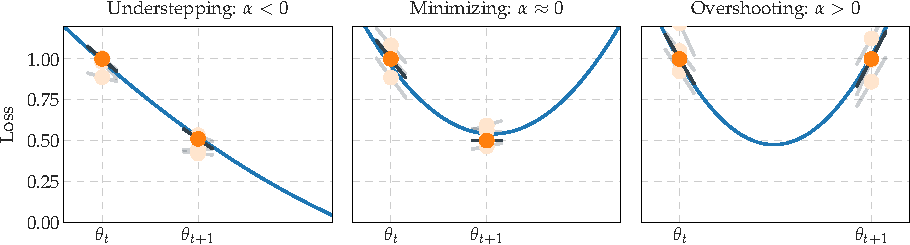
\includegraphics[width =
  \linewidth]{../repos/cockpit-paper/fig/12_alpha_explanation/output/alpha_explanation_thesis-wide}
  \caption{\textbf{Motivational sketch for the $\alpha$ quantity.} In each
    iteration of the optimizer we observe the loss function at two positions
    $\vtheta_{t}$ and $\vtheta_{t+1}$ (shown in
    \textcolor{sns_orange}{\ding{108}}). The black lines
    (\textcolor{TUdark}{\textbf{---}}) show the observed slope at this position,
    which we can get from projecting the gradients onto the current step
    direction $\vtheta_{t+1} - \vtheta_{t}$. Note, that all four observations
    (two loss and two slope values) are noisy, due to being computed on a
    mini-batch. With access to the individual losses and gradients (some samples
    shown in
    \textcolor{sns_orange_light}{\ding{108}}/\textcolor{TUgray}{\textbf{---}}),
    we can estimate their noise level and build a noise-informed quadratic fit
    (\textcolor{sns_blue}{\textbf{---}}). Using this fit, we determine whether
    the optimizer minimizes the local uni-variate loss (\textit{middle plot}), or
    whether we understep (\textit{left plot}) or overshoot (\textit{right plot})
    the minimum.}
  \label{cockpit::fig:alpha_explanation}
\end{figure*}

\subsubsection{Motivation}

The goal of the $\alpha$-quantity is to estimate and quantify the effect that a
selected learning rate has on the optimizer's steps. Consider the optimizer's
step at training iteration $t$. This parameter update from $\vtheta_{t}$ to
$\vtheta_{t+1}$ happens in a one-dimensional space, defined by the update
direction $\vtheta_{t+1} - \vtheta_{t}=\vs_t$. The update direction depends on
the update rule of the optimizer, \eg for \sgd with learning rate $\eta$ it is
simply $\vs_t =- \eta \vg_{\sB_t}(\vtheta_{t})$.

We build a noise-informed uni-variate quadratic approximation along this update
step ($\vtheta_{t} \to \vtheta_{t+1}$) based on the two noisy loss function
observations at $\vtheta_{t}$ and $\vtheta_{t+1}$ and the two noisy slope
observation at these two points. Examining this quadratic fit, we are able to
determine where on this parabola our optimizer steps. Standardizing this, we
express a step to the minimum of the loss in the update direction as $\alpha=0$.
Analogously, steps that end short of this minimum result in $\alpha<0$, and a
step over the minimum in $\alpha>0$. These three different scenarios are
illustrated in \Cref{cockpit::fig:alpha_explanation} also showing the underlying
observations that would lead to them. \Cref{cockpit::fig:LINE} shows the distribution of
$\alpha$-values for two very different optimization trajectories.

\subsubsection{Noisy Observations}

In order to build an approximation for the loss function in the update
direction, we leverage the four observations of the function (and its
derivative) that are available in each iteration. Due to the stochasticity of
deep learning optimization, we also take into account the noise-level of all
observations by estimating them. The first two observations are the mini-batch
training losses $\mathcal{L}_{\sB_t}(\vtheta_t),
\mathcal{L}_{\sB_{t+1}}(\vtheta_{t+1})$ at point $\vtheta_{t}$ and
$\vtheta_{t+1}$, which are computed in every standard training loop. The
mini-batch losses are averages over individual losses,
\begin{align*}
  \mathcal{L}_{\sB_t}(\vtheta_t)
  &=
    \E_{\sB_t}\left[ \ell(\vtheta_t) \right] = \frac{1}{|\sB_t|} \sum_{n \in \sB_t}
    \ell_n(\vtheta_t) \,,
  \\
  \mathcal{L}_{\sB_{t+1}}(\vtheta_{t+1})
  &=
    \E_{\sB_{t+1}}\left[ \ell(\vtheta_{t+1}) \right] = \frac{1}{|\sB_{t+1}|} \sum_{n \in \sB_{t+1}}
    \ell_n(\vtheta_{t+1})\,,
\end{align*}
and using these individual losses, we can also compute the variances to estimate
the noise-level of our loss observation,
\begin{align*}
  \Var_{\sB_{t}} \left[ \ell(\vtheta_t) \right]
  =&
     \left( \frac{1}{|\sB_t|} \sum_{n \in \sB_t} \ell_n(\vtheta_t)^2 \right)
     -
     \left( \frac{1}{|\sB_t|} \sum_{n \in \sB_t} \ell_n(\vtheta_t) \right)^2 \, ,
  \\
  \Var_{\sB_{t+1}} \left[ \ell(\vtheta_{t+1}) \right]
  =&
     \left( \frac{1}{|\sB_{t+1}|} \sum_{n \in \sB_{t+1}} \ell_n(\vtheta_{t+1})^2 \right)
     -
     \left( \frac{1}{|\sB_{t+1}|} \sum_{n \in \sB_{t+1}} \ell_n(\vtheta_{t+1}) \right)^2 \, .
\end{align*}
Similarly, we proceed with the slope in the update direction. To compute the
slope of the loss function in the direction of the optimizer's update $\vs_t$,
we project the current gradient along this update direction
\begin{align*}
  \E_{\sB_t} \left[\frac{\vs_t^\top \vg(\vtheta_t)}{\lVert \vs_t
  \rVert^2}\right]
  =&
     \frac{1}{|\sB_{t}|} \sum_{n\in \sB_t} \frac{\vs_t^\top \vg_n(\vtheta_t)}{\lVert
     \vs_t \rVert^2} \, ,
  \\
  \E_{\sB_{t+1}} \left[\frac{\vs_t^\top \vg(\vtheta_{t+1})}{\lVert \vs_t
  \rVert^2}\right]
  =&
     \frac{1}{|\sB_{t+1}|} \sum_{n\in \sB_{t+1}} \frac{\vs_t^\top \vg_n(\vtheta_{t+1})}{\lVert
     \vs_t \rVert^2} \, .
\end{align*}
Just like before, we can also compute the variance of this slope, by leveraging
individual gradients,
\begin{align*}
  &\Var_{\sB_t} \left[\frac{\vs_t^\top \vg(\vtheta_t)}{\lVert \vs_t
  \rVert^2}\right]
    \\
  &\quad=
     \frac{1}{|\sB_t|} \sum_{n\in B_t} \left( \frac{\vs_t^\top \vg_n(\vtheta_t)}{\lVert
     \vs_t \rVert^2} \right)^2
     -  \left( \frac{1}{|\sB_t|} \sum_{n\in \sB_t} \frac{\vs_t^\top
     \vg_n(\vtheta_t)}{\lVert \vs_t \rVert^2} \right)^2 \, ,
  \\
  &\Var_{\sB_{t+1}} \left[\frac{\vs_t^\top \vg(\vtheta_{t+1})}{\lVert \vs_t
  \rVert^2}\right]
    \\
  &\quad=
     \frac{1}{|\sB_{t+1}|} \sum_{n\in \sB_{t+1}} \left( \frac{\vs_t^\top \vg_n(\vtheta_{t+1})}{\lVert
     \vs_t \rVert^2} \right)^2
     -  \left( \frac{1}{|\sB_{t+1}|} \sum_{n\in \sB_{t+1}} \frac{\vs_t^\top
     \vg_n(\vtheta_{t+1})}{\lVert \vs_t \rVert^2} \right)^2 \, .
\end{align*}

\subsubsection{Quadratic Fit \& Normalization}

Using our (noisy) observations, we are now ready to build an approximation for
the loss as a function of the step size, which we will denote as $f(\tau)$. We
assume a quadratic function for $f$, which follows recent reports for the loss
landscape of neural networks \citep{xing2018walk}, \ie a function $f(\tau) = w_0
+ w_1 \tau + w_2 \tau^2$ parameterized by $\vw \in \R^3$. We further assume a
Gaussian likelihood of the form
\begin{align}
  \label{cockpit::eq:alpha_likelihood}
  p\left(\giventhat{\tilde{\vf}}{\vw, \mPhi}\right)
  =
  \mathcal{N}\left(\giventhat{\tilde{\vf}}{ \mPhi^\top \vw, \mLambda}\right)
\end{align}
for observations $\tilde{\vf}$ of the loss and its slope. The observation matrix
$\mPhi$ and the noise matrix of the observations $\mLambda$ are
\begin{align*}
  \mPhi = \begin{pmatrix}
    1 & 1 & 0 & 0 \\
    \tau_1 & \tau_2  & 1 & 1 \\
    \tau_1^2 & \tau_2^2 & 2\tau_1 &  2\tau_2
  \end{pmatrix}\,,
                                    \qquad \qquad
                                    \mLambda = \begin{pmatrix}
                                      \sigma_{\tilde{f}_1} & 0 & 0 & 0 \\ 0 & \sigma_{\tilde{f}_2} & 0 & 0  \\ 0
                                      & 0 & \sigma_{\tilde{f}'_1} & 0 \\ 0 & 0 & 0 & \sigma_{\tilde{f}'_2}
                                    \end{pmatrix} \, ,
\end{align*}
where $\tau$ denotes the position and $\sigma$ denotes the noise-level estimate
of the observation. The maximum likelihood solution of
\Cref{cockpit::eq:alpha_likelihood} for the parameters of our quadratic fit is given by
\begin{align}
  \label{cockpit::eq:alpha-feature-table}
  \vw = \left(\mPhi \mLambda^{-1}\mPhi^\top\right)^{-1}\mPhi \mLambda^{-1}
  \tilde{\vf} \, .
\end{align}
Once we have the quadratic fit of the uni-variate loss along the update
direction, we normalize the scales such that the resulting $\alpha$ expresses
the effective step taken by the optimizer sketched in
\Cref{cockpit::fig:alpha_explanation}.

\subsubsection{Usage}

The $\alpha$-quantity is related to recent line search approaches
\cite{mahsereci2017probabilistic,vaswani2019painless}. However, instead of searching for an
acceptable step by repeated attempts, we instead report the effect of the
current step size selection. This could, for example, be used to disentangle the
two optimization runs in \Cref{cockpit::fig:LINE}. Additionally, this information could
also be used to automatically adapt the learning rate during the training
process. But, as discussed in \Cref{cockpit::sec:alpha_exp}, it isn't trivial what the
``correct'' decision is, as it might depend on the optimization problem, the
training phase, and other factors. Having this $\alpha$-quantity can, however,
provide more insight into what kind of steps are used in well-tuned runs with
traditional optimizers such as \sgd.

%%% Local Variables:
%%% mode: latex
%%% TeX-master: "../thesis"
%%% End:

\subsection{\cabs Criterion: Coupling Adaptive Batch Sizes with Learning Rates
  (\robustInlinecode{CABS})}\label{cockpit::app:cabs}

The \cabs criterion, proposed by \citet{balles2017coupling}, can be used to adapt the
mini-batch size during training with \sgd. It relies on the gradient noise and
approximately optimizes the objective's expected gain per cost. The adaptation
rule is (with learning rate $\eta$)
\begin{equation}
  \label{cockpit::eq:cabs-theoretical}
  |\sB| \leftarrow \eta \frac{\Tr(\mSigma_{\pdata}(\vtheta))}{\gL_{{\pdata}}(\vtheta)}\,,
\end{equation}
and the practical implementation approximates $ \gL_{{\pdata}}(\vtheta) \approx
\gL_{\sB}(\vtheta)$and $\Tr(\mSigma_{\pdata}(\vtheta)) \approx
\nicefrac{(|\sB|-1)}{|\sB|} \Tr(\hat{\mSigma}_\sB(\vtheta))$ (compare equations
(10, 22) and first paragraph of Section 4 in \citep{balles2017coupling}). This
yields the quantity computed in \cockpit's \inlinecode{CABS} instrument,
\begin{align}
  \label{cockpit::eq:cabs-feature-table}
  |\sB| &\leftarrow \eta \frac{
          \frac{1}{|\sB|}
          \sum_{j=1}^D \sum_{n\in\sB}
          \left[
          \vg_n(\vtheta) - \vg_{\sB}(\vtheta)
          \right]_j^2
          }{
          \gL_{\sB}(\vtheta)
          }\,.
\end{align}

\subsubsection{Usage}

The \cabs criterion suggests a batch size which is optimal
under certain assumptions. This suggestion can support practitioners in the
batch size selection for their deep learning task.

%%% Local Variables:
%%% mode: latex
%%% TeX-master: "../thesis"
%%% End:

\subsection{Early-stopping Criterion for SGD
  (\robustInlinecode{EarlyStopping})}\label{cockpit::app:early-stopping}

The empirical risk $\gL_{\sD}(\vtheta)$, and the mini-batch loss
$\gL_{\sB}(\vtheta)$ are only estimators of the target objective
$\gL_{\pdata}(\vtheta)$. \citet{mahsereci2017early} motivate
$p(\giventhat{\vg_{\sB,\sD}(\vtheta)}{\vg_{\pdata}(\vtheta) = \vzero})$ as a measure for
detecting noise in the finite datasets $\sB, \sD$ due to sampling from $\pdata$.
They propose an evidence-based (EB) criterion for early stopping the training
procedure based on mini-batch statistics, and model $p(\vg_{\sB}(\vtheta))$ with
a sampled diagonal variance approximation (compare
\Cref{cockpit::eq:cheat-sheet-risk-gradient-diagonal-variance-estimator}),
\begin{equation}
  p(\vg_{\sB}(\vtheta))
  \approx \prod_{j=1}^D  \gN\left(
    \giventhat{
      \vg_{\sB}(\vtheta)
    }{
      \left[\vg_{\pdata}(\vtheta)\right]_j,
      \frac{\left[ \hat{\mSigma}_\sB(\vtheta)\right]_{j,j}}{|\sB|}
    }
  \right)\,.
\end{equation}
Their \sgd stopping criterion is
\begin{subequations}
  \begin{align}
    \frac{2}{D} \left[ \log p(\vg_{\sB}(\vtheta))
    - \E_{\vg_{\sB}(\vtheta) \sim p(\vg_{\sB}(\vtheta))} \left[ \log p(\vg_{\sB}(\vtheta))\right]
    \right]
    &> 0\,,
      \intertext{and translates into}
      1 - \frac{|\sB|}{D} \sum_{d=1}^D \frac{
      \left[ \vg_{\sB}(\vtheta)\right]_d^2
      }{
      \left[ \hat{\mSigma}_\sB(\vtheta)\right]_{d,d}
      }
    &> 0\,,
    \\
    1 - \frac{|\sB|}{D} \sum_{d=1}^D \frac{
    \left[ \vg_{\sB}(\vtheta)\right]_d^2
    }{
    \frac{1}{|\sB| - 1}
    \sum_{n\in \sB}
    \left[
    \vg_n(\vtheta) - \vg_{\sB}(\vtheta)
    \right]_d^2
    }
    &> 0\,,
    \\
    \label{cockpit::eq:early-stopping-feature-table}
    1 - \frac{|\sB| (|\sB| - 1)}{D} \sum_{d=1}^D \frac{
    \left[ \vg_{\sB}(\vtheta)\right]_d^2
    }{
    \left(
    \sum_{n\in \sB}
    \left[
    \vg_n(\vtheta)
    \right]_d^2
    \right)
    - |\sB|
    \left[
    \vg_{\sB}(\vtheta)
    \right]_d^2
    }
    &> 0\,.
  \end{align}
\end{subequations}
\cockpit's \inlinecode{EarlyStopping} quantity computes the left side of
\Cref{cockpit::eq:early-stopping-feature-table}.

\subsubsection{Usage}

\cockpit's \inlinecode{EarlyStopping} quantity can inform practitioners that
training is about to be completed and the model might be at risk of overfitting.

%%% Local Variables:
%%% mode: latex
%%% TeX-master: "../thesis"
%%% End:

\subsection{Individual Gradient Element Histograms (\robustInlinecode{GradHist1d},
  \robustInlinecode{GradHist2d})}
For the $|\sB| \times D$ individual gradient elements, \cockpit's
\inlinecode{GradHist1d} instrument displays a histogram of
\begin{equation}
  \label{cockpit::eq:app-grad-hist-1d}
  \left\{
    [\vg_n(\vtheta)]_d
  \right\}_{n\in\sB,d=1,\dots, D}\,.
\end{equation}
\cockpit's \inlinecode{GradHist2d} instrument displays a two-dimensional histogram
of the $|\sB| \times D$ tuples
\begin{equation}
  \label{cockpit::eq:app-grad-hist-2d}
  \left\{
    \left(
      [\vtheta]_d,
      [\vg_n(\vtheta)]_d
    \right)
  \right\}_{n\in\sB,d=1,\dots, D}\,
\end{equation}
and the marginalized one-dimensional histograms over the parameter and gradient
axes.

\subsubsection{Usage}

\Cref{cockpit::sec:misscaled_data_exp,cockpit::sec:vanishing_gradient_exp}
provide use cases (identifying data pre-processing issues and vanishing
gradients) for both the gradient histogram as well as its layer-wise extension.

%%% Local Variables:
%%% mode: latex
%%% TeX-master: "../thesis"
%%% End:

\subsection{Gradient Tests (\robustInlinecode{NormTest},
  \robustInlinecode{InnerTest},
  \robustInlinecode{OrthoTest})}\label{cockpit::app:gradient_tests}

\citet{bollapragada2017adaptive} and \citet{byrd2012sample} propose batch size adaptation
schemes based on the gradient noise. They formulate geometric constraints
between population and mini-batch gradient and accessible approximations that
can be probed to decide whether the mini-batch size should be increased. Because
mini-batches are \iid from $\pdata$, it holds that
\begin{subequations}
  \label{cockpit::eq:iid-sampling-expectation}
  \begin{align}
    \E\left[\vg_{\sB}(\vtheta) \right]
    &=
      \vg_{\pdata}(\vtheta),
    \\
    \E\left[ \vg_{\sB}(\vtheta)^\top \vg_{\pdata}(\vtheta)  \right]
    &=
      \lVert \vg_{\pdata}(\vtheta)  \rVert^2.
  \end{align}
\end{subequations}

The above works propose enforcing other weaker similarity in expectation during
optimization. These geometric constraints reduce to basic vector geometry (see
\Cref{cockpit::subfig:gradient-test-sketch1} for an overview of the relevant
vectors). We recall their formulation here for consistency and derive the
practical versions, which can be computed from training observables and are used
in \cockpit (consult \Cref{cockpit::subfig:gradient-test-sketch2} for the
visualization).

\begin{figure*}[ht]
  \centering
  \begin{subfigure}[t]{0.59\linewidth}
    \centering
    \tikzexternalenable
    \begin{tikzpicture}[rotate=5, >=latex, very thick, xscale = 1., yscale =
      1.25]

      % node style
      \tikzset{my label style/.style={fill=white, fill opacity=0.5, text
          opacity=1, font=\footnotesize}}


      % expected risk gradient
      \draw[->, ultra thick] (0,0) to node [midway, anchor=north west, my label
      style] {$\vg_{\pdata}$} (7,0);

      % mini-batch gradient
      \draw[->] (0,0) to node [midway, anchor=south east, my label style]
      {$\vg_{\sB}$} (6,3);
      \draw[->, >=latex] (0,0) -- (6,3);

      % right angle
      % \draw (6,0) rectangle ++(-0.15,0.15);

      % residual
      \draw[->, sns_blue] (7,0) to node [midway, right, anchor=south west, my label
      style] {$\vg_{\sB} - \vg_{\pdata}$} (6,3);

      % projection
      \draw[->, sns_orange] (0,0) to node [midway, above, anchor=south east, my label
      style] {$\mathrm{proj}_{\vg_{\pdata}}\left(\vg_{\sB}\right)$} (6,0);

      % orthogonal residual
      \draw[->, sns_green] (6,0) to node [midway, left, anchor=north east, my label
      style] {$\vg_{\sB} - \mathrm{proj}_{\vg_{\pdata}}\left(\vg_{\sB}\right)$} (6,3);
    \end{tikzpicture}
    \tikzexternaldisable
    \caption{Relevant vectors}
    \label{cockpit::subfig:gradient-test-sketch1}
  \end{subfigure}
  \begin{subfigure}[t]{0.39\linewidth}
    \centering
    \tikzexternalenable
    \begin{tikzpicture}[>=latex, very thick, xscale = 2, yscale = 2]
      \clip (-1,0) rectangle (1,2);

      % expected risk gradient
      % \draw[->, ultra thick] (0,0) to (0,1);
      % target indicator
      \draw[ultra thick] (0,0.9) to (0,1.1);
      \draw[ultra thick] (-0.1,1) to (0.1,1);

      % norm test
      \pgfmathsetmacro{\normTestRadius}{0.5}
      \filldraw [fill=sns_blue, opacity=0.4] (0,1) circle (\normTestRadius);

      % inner product test
      \pgfmathsetmacro{\innerProductWidth}{0.2}
      \filldraw [fill=sns_orange, opacity=0.4] (-2,1 - \innerProductWidth) rectangle
      (2,1 + \innerProductWidth);

      % orthogonality test
      \pgfmathsetmacro{\orthogonalityTestWidth}{0.3}
      \filldraw [fill=sns_green, opacity=0.4] (-\orthogonalityTestWidth, 0) rectangle
      (\orthogonalityTestWidth, 2);

      % norm test label
      \draw[ultra thick, <->, sns_blue] (0,1) to ++(45:\normTestRadius) node [above, right] {\footnotesize $\theta_{\text{norm}}$};

      % inner product test label
      \draw[ultra thick, <->, sns_orange] (-0.75, 1 - \innerProductWidth) to ++(0, 2 *\innerProductWidth) node [above] {\footnotesize $2 \theta_{\text{inner}}$};

      % orthogonality test label
      \draw[ultra thick, <->, sns_green] (-\orthogonalityTestWidth0, 0.2) to ++(2 *\orthogonalityTestWidth, 0.) node [right] {\footnotesize $2 \nu_{\text{ortho}}$};

      % acute angle test
      % \pgfmathsetmacro{\acuteAngle}{30}
      % \pgfmathsetmacro{\initAngle}{90 - \acuteAngle}
      % \pgfmathsetmacro{\endAngle}{90 + \acuteAngle}
      % \pgfmathsetmacro{\acuteAngleRadius}{3}

      % \filldraw [fill=black, opacity=0.2] (0,0) --
      % (\initAngle:\acuteAngleRadius) arc
      % (\initAngle:\endAngle:\acuteAngleRadius) -- cycle;
    \end{tikzpicture}
    \tikzexternaldisable
    \caption{\cockpit's gradient test visualization.}
    \label{cockpit::subfig:gradient-test-sketch2}
  \end{subfigure}
  \caption{\textbf{Conceptual sketch for gradient tests.}
    \subfigref{cockpit::subfig:gradient-test-sketch1} Relevant vectors to
    formulate the geometric constraints between population and mini-batch
    gradient probed by the gradient tests.
    \subfigref{cockpit::subfig:gradient-test-sketch2} Gradient test
    visualization in \cockpit.}
  \label{cockpit::fig:gradient-tests-sketch}
\end{figure*}

\subsubsection{Usage}

All three gradient tests describe the noise level of the gradients.
\citet{bollapragada2017adaptive} and \citet{byrd2012sample} adapt the batch size
so that the proposed geometric constraints are fulfilled. Practitioners can use
the combined gradient test plot, \ie top center plot in
\Cref{cockpit::fig:showcase}, to monitor gradient noise during training and
adjust hyperparameters such as the batch size.


\subsubsection{Norm Test (\robustInlinecode{NormTest})}\label{cockpit::app:norm-test}
The norm test \citep{byrd2012sample} constrains the residual norm $\lVert
\vg_{\sB}(\vtheta) - \vg_{\pdata}(\vtheta) \rVert$, rescaled by $\lVert
\vg_{\pdata}(\vtheta) \rVert$. This gives rise to a standardized ball of radius
$\theta_{\text{norm}} \in (0, \infty)$ around the population gradient, where the
mini-batch gradient should reside. \citet{byrd2012sample} set
$\theta_{\text{norm}} = 0.9$ in their experiments and increase the batch size if
(in the practical version, see below) the following constraint is not fulfilled
\begin{subequations}
  \begin{align}
    \label{cockpit::eq:norm-test-constraint}
    \E\left[ \frac{ \left\lVert \vg_{\sB}(\vtheta) - \vg_{\pdata}(\vtheta)
    \right\rVert^2 }{\left\lVert \vg_{\pdata}(\vtheta) \right\rVert^2} \right]
    \le
    \theta_{\text{norm}}^2\,.
  \end{align}
  Instead of taking the expectation over mini-batches, \citet{byrd2012sample} note
  that the above will be satisfied if
  \begin{equation}
    \label{cockpit::eq:norm-test-individual}
    \frac{1}{|\sB|} \E\left[ \frac{ \left\lVert \vg_n(\vtheta) - \vg_{\pdata}(\vtheta)
        \right\rVert^2 }{\left\lVert \vg_{\pdata}(\vtheta) \right\rVert^2} \right]
    \le \theta_{\text{norm}}^2\,.
  \end{equation}
\end{subequations}
They propose a practical form of this test,
\begin{subequations}
  \begin{equation}
    \label{cockpit::eq:norm-test-practical-proposed}
    \frac{1}{|\sB| (|\sB| - 1)} \frac{\sum_{n \in \sB} \left\lVert \vg_n(\vtheta) -
        \vg_{\sB}(\vtheta) \right\rVert^2}{\left\lVert
        \vg_{\sB}(\vtheta)\right\rVert^2} \le \theta_{\text{norm}}^2\,,
  \end{equation}
  which can be computed from mini-batch statistics. Rearranging
  \begin{align}
    \sum_{n \in \sB} \left\lVert \vg_n(\vtheta) - \vg_{\sB}(\vtheta) \right\rVert^2
    &= \left( \sum_{n \in \sB} \left\lVert \vg_n(\vtheta) \right\rVert^2 \right) - |\sB|
      \left\lVert \vg_{\sB}(\vtheta) \right\rVert^2\,,
  \end{align}
  we arrive at
  \begin{align}
    \label{cockpit::eq:norm-test-feature-table}
    \frac{1}{|\sB| (|\sB| - 1)} \left[ \frac{ \sum_{n \in \sB} \left\lVert
    \vg_n(\vtheta) \right\rVert^2 }{\left\lVert
    \vg_{\sB}(\vtheta)\right\rVert^2} - |\sB| \right] &\le
                                                        \theta_{\text{norm}}^2
  \end{align}
\end{subequations}
that leverages the norm of both the mini-batch and the individual gradients,
which can be aggregated over parameters during a backward pass. \cockpit's
\inlinecode{NormTest} corresponds to the maximum radius $\theta_{\text{norm}}$
for which the above inequality holds.

\subsubsection{Inner Product Test
  (\robustInlinecode{InnerTest})}\label{cockpit::app:inner-product-test}
The inner product test \citep{bollapragada2017adaptive} constrains the
projection of $\vg_{\sB}(\vtheta)$ onto $\vg_{\pdata}(\vtheta)$ (compare
\Cref{cockpit::subfig:gradient-test-sketch1}),
\begin{align}
  \label{cockpit::eq:inner-product-projection}
  \mathrm{proj}_{\vg_{\pdata}(\vtheta)}\left(\vg_{\sB}(\vtheta)\right)
  :=
  \frac{\vg_{\sB}(\vtheta)^\top \vg_{\pdata}(\vtheta)}{\left\lVert
  \vg_{\pdata}(\vtheta) \right\rVert^2} \vg_{\pdata}(\vtheta)\,,
\end{align}
rescaled by $\lVert \vg_{\pdata}(\vtheta) \rVert$. This restricts the mini-batch
gradient to reside in a standardized band of relative width
$\theta_{\text{inner}}\in (0, \infty)$ around the population risk gradient.
\citet{bollapragada2017adaptive} use $\theta_{\text{inner}} = 0.9$ (in the practical
version, see below) to adapt the batch size if the parallel component's variance
does not satisfy the condition
\begin{subequations}
  \begin{align}
    \label{cockpit::eq:inner-product-test}
    \Var\left( \frac{\vg_{\sB}(\vtheta)^\top \vg_{\pdata}(\vtheta)}{\left\lVert
    \vg_{\pdata}(\vtheta) \right\rVert^2} \right)
    &= \E\left[ \left( \frac{\vg_{\sB}(\vtheta)^\top \vg_{\pdata}(\vtheta)}{\left\lVert
      \vg_{\pdata}(\vtheta) \right\rVert^2}  -1 \right)^2 \right]
      \le \theta_{\text{inner}}^2
  \end{align}
  (note that by \Cref{cockpit::eq:iid-sampling-expectation} we have $\E[
    \nicefrac{\vg_{\sB}(\vtheta)^\top \vg_{\pdata}(\vtheta)}{\left\lVert \vg_{\pdata}(\vtheta)
      \right\rVert^2} ] = 1 $). \citet{bollapragada2017adaptive} bound
  \Cref{cockpit::eq:inner-product-test} by the individual gradient variance,
  \begin{align}
    \label{cockpit::eq:inner-product-test-individual}
    \begin{split}
      &\frac{1}{|\sB|}\Var\left( \frac{\vg_n(\vtheta)^\top \vg_{\pdata}(\vtheta)}{\left\lVert
      \vg_{\pdata}(\vtheta) \right\rVert^2}\right)
      \\
      &\qquad =
      \frac{1}{|\sB|} \E \left[ \left( \frac{\vg_n(\vtheta)^\top \vg_{\pdata}(\vtheta) }{\left\lVert
      \vg_{\pdata}(\vtheta) \right\rVert^2} - 1    \right)^2  \right] \le \theta_{\text{inner}}^2\,.
    \end{split}
  \end{align}
\end{subequations}
They then propose a practical form of \Cref{cockpit::eq:inner-product-test-individual},
which uses the mini-batch sample variance,
\begin{subequations}
  \begin{align}
    \label{cockpit::eq:inner-product-test-practical}
    \begin{split}
    &\frac{1}{|\sB|} \Var\left( \frac{\vg_n(\vtheta)^\top \vg_{\sB}(\vtheta)}{\left\lVert
    \vg_{\sB}(\vtheta)\right\rVert^2}\right)
      \\
      &\qquad
    = \frac{1}{|\sB| (|\sB| - 1)}\left[  \sum_{n\in \sB}  \left( \frac{\vg_n(\vtheta)^\top \vg_{\sB}(\vtheta)}{\left\lVert
    \vg_{\sB}(\vtheta)\right\rVert^2} - 1    \right)^2  \right]
    \le \theta_{\text{inner}}^2\,.
    \end{split}
  \end{align}
  Expanding
  \begin{align}
    \label{cockpit::eq:inner-product-test-practical-rewrite}
    \sum_{n\in \sB}  \left( \frac{\vg_n(\vtheta)^\top \vg_{\sB}(\vtheta)}{\left\lVert
    \vg_{\sB}(\vtheta)\right\rVert^2} - 1    \right)^2
    &=
      \frac{\sum_{n\in \sB}  \left( \vg_n(\vtheta)^\top \vg_{\sB}(\vtheta)\right)^2}{\left\lVert
      \vg_{\sB}(\vtheta)\right\rVert^4} - |\sB|
  \end{align}
  and inserting \Cref{cockpit::eq:inner-product-test-practical-rewrite} into
  \Cref{cockpit::eq:inner-product-test-practical} yields
  \begin{align}
    \label{cockpit::eq:inner-product-test-feature-table}
    \frac{1}{|\sB| (|\sB| - 1)}
    \left[   \frac{\sum_{n\in \sB}  \left( \vg_n(\vtheta)^\top \vg_{\sB}(\vtheta)\right)^2}{\left\lVert
    \vg_{\sB}(\vtheta)\right\rVert^4} - |\sB|\right]
    &\le \theta_{\text{inner}}^2\,.
  \end{align}
\end{subequations}
It relies on pairwise scalar products between individual gradients, which can be
aggregated over layers during backpropagation. \cockpit's \inlinecode{InnerTest}
quantity computes the maximum band width $\theta_{\text{inner}}$ that satisfies
\Cref{cockpit::eq:inner-product-test-feature-table}.

\subsubsection{Orthogonality Test (\robustInlinecode{OrthoTest})}\label{cockpit::app:orthogonality-test}
In contrast to the inner product test (\Cref{cockpit::app:inner-product-test})
which constrains the projection (\Cref{cockpit::eq:inner-product-projection}),
the orthogonality test \citep{bollapragada2017adaptive} constrains the
orthogonal part (see \Cref{cockpit::fig:gradient-tests-sketch} (a))
\begin{align}
  \label{cockpit::eq:orthogonality-projection}
  \vg_{\sB}(\vtheta)
  -
  \mathrm{proj}_{\vg_{\pdata}(\vtheta)}\left(\vg_{\sB}(\vtheta)\right)\,,
\end{align}
rescaled by $\lVert \vg_{\pdata}(\vtheta) \rVert$. This restricts the mini-batch
gradient to a standardized band of relative width $\nu_{\text{ortho}} \in (0,
\infty)$ parallel to the population gradient. \citet{bollapragada2017adaptive} use $\nu
= \tan(80^{\circ}) \approx 5.84$ (in the practical version, see below) to adapt
the batch size if the following condition is violated,
\begin{subequations}
  \begin{align}
    \label{cockpit::eq:orthogonality-test-constraint}
    \E\left[
    \left\lVert
    \frac{
    \vg_{\sB}(\vtheta)
    -
    \mathrm{proj}_{\vg_{\pdata}(\vtheta)}\left(\vg_{\sB}(\vtheta)\right)
    }{
    \lVert \vg_{\pdata}(\vtheta) \rVert
    }
    \right\rVert^2
    \right]
    \le \nu^2_{\text{ortho}}\,.
  \end{align}
  Expanding the norm, and inserting \Cref{cockpit::eq:inner-product-projection}, this
  simplifies to
  \begin{align}
    \begin{split}
      \E \left[ \left\lVert \frac{ \vg_{\sB}(\vtheta) }{ \lVert \vg_{\pdata}(\vtheta)
      \rVert } - \frac{ \vg_{\sB}(\vtheta)^\top \vg_{\pdata}(\vtheta) }{ \lVert
      \vg_{\pdata}(\vtheta) \rVert^2 } \frac{ \vg_{\pdata}(\vtheta) }{ \lVert
      \vg_{\pdata}(\vtheta) \rVert} \right\rVert^2 \right] &\le
                                                        \nu^2_{\text{ortho}}\,,
      \\
      \E\left[ \frac{ \lVert \vg_{\sB}(\vtheta) \rVert^2 }{ \lVert
      \vg_{\pdata}(\vtheta) \rVert^2 } - \frac{ \left( \vg_{\sB}(\vtheta)^\top
      \vg_{\pdata}(\vtheta) \right)^2 }{ \lVert \vg_{\pdata}(\vtheta) \rVert^4 }
      \right] &\le \nu^2_{\text{ortho}}\,.
    \end{split}
  \end{align}
  \citet{bollapragada2017adaptive} bound this inequality with individual gradients,
  \begin{align}
    \frac{1}{|\sB|}
    \E \left[
    \left\lVert
    \frac{
    \vg_n(\vtheta)
    }{
    \lVert
    \vg_{\pdata}(\vtheta)
    \rVert^2
    }
    -
    \frac{
    \vg_n(\vtheta)^\top
    \vg_{\pdata}(\vtheta)
    }{
    \lVert
    \vg_{\pdata}(\vtheta)
    \rVert^2
    }
    \frac{
    \vg_{\pdata}(\vtheta)
    }{
    \left\lVert
    \vg_{\pdata}(\vtheta)
    \right\rVert}
    \right\rVert^2
    \right]
    &\le \nu^2_{\text{ortho}}\,.
  \end{align}
\end{subequations}
They propose the practical form
\begin{subequations}
  \begin{align}
    \frac{1}{|\sB|(|\sB|-1)}
    \E\left[
    \left\lVert
    \frac{
    \vg_n(\vtheta)
    }{
    \lVert
    \vg_{\sB}(\vtheta)
    \rVert
    }
    -
    \frac{
    \vg_n(\vtheta)^\top
    \vg_{\sB}(\vtheta)
    }{
    \lVert
    \vg_{\sB}(\vtheta)
    \rVert^2
    }
    \frac{
    \vg_{\sB}(\vtheta)
    }{
    \left\lVert
    \vg_{\sB}(\vtheta)
    \right\rVert}
    \right\rVert^2
    \right]
    &\le \nu^2_{\text{ortho}}\,,
  \end{align}
  which simplifies to
  \begin{align}
    \label{cockpit::eq:orthogonality-test-feature-table}
    \frac{1}{|\sB| (|\sB| - 1)}
    \sum_{n \in \sB }
    \left(
    \frac{
    \lVert
    \vg_n(\vtheta)
    \rVert^2
    }{
    \lVert
    \vg_{\sB}(\vtheta)
    \rVert^2
    }
    -
    \frac{
    \left(
    \vg_n(\vtheta)^\top
    \vg_{\sB}(\vtheta)
    \right)^2
    }{
    \lVert
    \vg_{\sB}(\vtheta)
    \rVert^4
    }
    \right)
    &\le \nu^2_{\text{ortho}}\,.
  \end{align}
\end{subequations}
It relies on pairwise scalar products between individual gradients which can be
aggregated over layers during a backward pass. \cockpit's \inlinecode{OrthoTest}
quantity computes the maximum band width $\nu_{\text{ortho}}$ which satisfies
\Cref{cockpit::eq:orthogonality-test-feature-table}.

\subsubsection{Relation to Acute Angle Test}

Recently, a novel ``acute angle test'' was proposed by
\citet{bahamou2019dynamic}. While the theoretical constraint between
$\vg_{\sB}(\vtheta)$ and $\vg_{\pdata}(\vtheta)$ differs from the orthogonality
test, the practical versions coincide. Hence, we do not incorporate the acute
angle here.

%%% Local Variables:
%%% mode: latex
%%% TeX-master: "../thesis"
%%% End:

\subsection{Hessian Maximum Eigenvalue
  (\robustInlinecode{HessMaxEV})}\label{cockpit::app:max-ev}

The Hessian's maximum eigenvalue $\lambda_{\text{max}}(\mH_{\sB}(\vtheta))$ is
computed with an iterative eigensolver from Hessian-vector products through
\pytorch's automatic differentiation \citep{pearlmutter1994fast}. Like
\citet{yao2020pyhessian}, we employ power iterations with similar
\href{https://github.com/amirgholami/PyHessian/blob/0f7e0f63a0f132998608013351ba19955fc9d861/pyhessian/hessian.py#L111-L158}{default
  stopping parameters} (stop after at most 100 iterations, or if the iterate
does converged with a relative and absolute tolerance of $10^{-3}, 10^{-6}$,
respectively) to compute $\lambda_{\text{max}}(\mH_{\sB}(\vtheta))$ through the
\inlinecode{HessMaxEV} quantity in \cockpit.

In principle, more sophisticated eigensolvers (for example Arnoldi's method)
could be applied to converge in fewer iterations or compute eigenvalues other
than the leading ones. \citet{warsa2004krylov} empirically demonstrate that the
FLOP ratio between power iteration and implicitly restarted Arnoldi method can
reach values larger than $100$. While we can use such a beneficial method on a
CPU through
\href{https://docs.scipy.org/doc/scipy/reference/generated/scipy.sparse.linalg.eigsh.html} {\texttt{scipy.sparse.linalg.eigsh}}
we are restricted to the GPU-compatible power iteration for GPU training. We
expect that extending the support of popular machine learning libraries like
\pytorch for such iterative eigensolvers on GPUs can help to save computation
time.

\begin{equation}
  \label{cockpit::eq:hess-max-ev-feature-table}
  \lambda_{\text{max}}(\mH_{\sB}(\vtheta))
  =
  \max_{\lVert \vv \rVert_2 = 1} \lVert \mH_{\sB}(\vtheta)\vv \rVert_2
  =
  \max_{\vv \in \sR^D} \frac{\vv^\top \mH_{\sB}(\vtheta) \vv}{\vv^\top \vv}.
\end{equation}

\subsubsection{Usage}

The Hessian's maximum eigenvalue describes the loss surface's sharpest direction
and thus provides an understanding of the current loss landscape. Additionally,
in convex optimization, the largest Hessian eigenvalue crucially determines the
appropriate step size \citep{schmidt2014convergence}. In
\Cref{cockpit::sec:showcase}, we can observe that although training seems stuck
in the very first few iterations progress is visible when looking at the maximum
Hessian eigenvalue.


%%% Local Variables:
%%% mode: latex
%%% TeX-master: "../thesis"
%%% End:

\subsection{Hessian Trace
  (\robustInlinecode{HessTrace})}\label{cockpit::app:hessian-trace}

In comparison to \citet{yao2020pyhessian}, who leverage Hessian-vector products
\citep{pearlmutter1994fast} to estimate the Hessian trace, we compute the exact
value $\Tr(\mH_{\sB}(\vtheta))$ with the \inlinecode{HessTrace} quantity in
\cockpit by aggregating the output of \backpack's
\href{https://docs.backpack.pt/en/master/extensions.html#backpack.extensions.DiagHessian}{\inlinecode{DiagHessian}}
extension, which computes the diagonal entries of $\mH_{\sB}(\vtheta)$.
Alternatively, the trace can also be estimated with the \ggn matrix, or an
MC-sampled approximation thereof.

\subsubsection{Usage}

The Hessian trace equals the sum of the eigenvalues and thus provides a notion
of ``average curvature'' of the current loss landscape. It has long been
theorized and discussed that curvature and generalization performance may be
linked \cite[\eg]{hochreiter1997flat}.

%%% Local Variables:
%%% mode: latex
%%% TeX-master: "../thesis"
%%% End:

\subsection{Takeuchi Information Criterion (\robustInlinecode{TICDiag},
  \robustInlinecode{TICTrace})}\label{cockpit::app:tic}

Recent work by \citet{thomas2020interplay} suggests that optimizer convergence
speed and generalization is mainly influenced by curvature and gradient noise;
and hence their interaction is crucial to understand the generalization and
optimization behavior of deep neural networks. They reinvestigate the Takeuchi
Information criterion \citep{takeuchi1976distribution}, an estimator for the
generalization gap in overparameterized maximum likelihood estimation. At a
local minimum $\vtheta_\star$, the generalization gap is estimated by the TIC
\begin{equation}
  \label{cockpit::eq:tic-theory}
  \frac{1}{|\sD|}
  \Tr
  \left(
    \mH_{\pdata}(\vtheta_\star)^{-1}
    \mK_{\pdata}(\vtheta_\star)
  \right)\,,
\end{equation}
where $\mH_{\pdata}(\vtheta_\star)$ is the population Hessian and
$\mK_{\pdata}(\vtheta_\star)$ is the gradient's uncentered second moment,
\begin{equation*}
  \mK_{\pdata}(\vtheta_\star)
  = \int
  \nabla_{\vtheta_{\star}}\ell(f_{\vtheta_{\star}}( \vx), \vy)
  \left(
    \nabla_{\vtheta_{\star}}\ell(f_{\vtheta_{\star}}( \vx), \vy)
  \right)^\top \pdata(\vx, \vy)
  \diff\vx\diff\vy.
\end{equation*}
Both matrices are inaccessible in practice. In their experiments,
\citet{thomas2020interplay} propose the approximation
$\nicefrac{\Tr(\mK)}{\Tr(\mH)}$ for $\Tr(\mH^{-1} \mK)$. They also replace the
Hessian by the Fisher as it is easier to compute. With these practical
simplifications, they investigate the TIC of trained neural networks where the
curvature and noise matrix are evaluated on a large dataset.

The TIC provided in \cockpit differs from this setting, since by design we want
to observe quantities during training, while avoiding additional model
predictions. Also, \backpack provides access to the Hessian; hence we don't need
to use the Fisher. We propose the following two approximations of the TIC from a
mini-batch:
\begin{itemize}
\item \inlinecode{TICTrace}: uses the approximation of \citet{thomas2020interplay} which
  replaces the matrix-product trace by the product of traces,
  \begin{align}
    \label{cockpit::eq:tic-trace-feature-table}
    \frac{
    \Tr\left(
    \mK_{\sB}(\vtheta)
    \right)
    }{
    \Tr\left(
    \mH_{\sB}(\vtheta)
    \right)
    }
    =
    \frac{
    \frac{1}{|\sB|}
    \sum_{n\in\sB}
    \lVert
    \vg_{n}(\vtheta)
    \rVert^2
    }{
    \Tr\left(
    \mH_{\sB}(\vtheta)
    \right)
    }\,.
  \end{align}
\item \inlinecode{TICDiag}: uses a diagonal approximation of the Hessian, which
  is cheap to invert,
  \begin{align}
    \label{cockpit::eq:tic-diag-feature-table}
    \begin{split}
      &\Tr\left(
        \diag\left(
        \mH_{\sB}(\vtheta)
        \right)^{-1}
        \mK_{\sB}(\vtheta)
        \right)
      \\
      &\qquad
        =
        \frac{1}{|\sB|}
        \sum_{d=1}^D
        \left[
        \mH_\sB(\vtheta)
        \right]_{d,d}^{-1}
        \left[
        \sum_{n\in\sB}
        \vg_{n}(\vtheta)^{\odot 2}
        \right]_{d}\,.
    \end{split}
  \end{align}
\end{itemize}

\subsubsection{Usage}

The TIC is a proxy for the generalization gap, see \citet{thomas2020interplay}.

%%% Local Variables:
%%% mode: latex
%%% TeX-master: "../thesis"
%%% End:

\subsection{Gradient Signal-to-noise Ratio (\robustInlinecode{MeanGSNR})}
\label{cockpit::app:mean-gsnr}
The gradient signal-to-noise ratio $\mathrm{GSNR}(\left[ \vtheta \right]_d) \in
\sR$ for a single parameter $\left[ \vtheta \right]_d$ is defined as
\begin{align}
  \label{cockpit::eq:gsnr-definition}
  \mathrm{GSNR}(\left[ \vtheta \right]_d)
  =
  \frac{
  \E_{(\vx, \vy)\sim P}\left[
  \left[
  \nabla_\vtheta\ell(f_{\vtheta}(\vx), \vy)
  \right]_d
  \right]^2
  }{
  \Var_{(\vx, \vy)\sim P}\left[
  \left[
  \nabla_\vtheta \ell(f_{\vtheta}(\vx), \vy)
  \right]_d
  \right]
  }
  =
  \frac{
  \left[
  \vg_{P}(\vtheta)
  \right]^2_d
  }{
  \left[
  \mSigma_P(\vtheta)
  \right]_{d,d}
  }\,.
\end{align}
\begin{subequations}
  \citet{liu2020understanding} use it to explain generalization properties of models
  in the early training phase. We apply their estimation to mini-batches,
  \begin{align}
    \label{cockpit::eq:gsnr-mini-batch}
    \mathrm{GSNR}(\left[ \vtheta \right]_d)
    &\approx
      \frac{
      \left[
      \vg_{\sB}(\vtheta)
      \right]_d^2
      }{
      \frac{|\sB| - 1}{|\sB|}
      \left[
      \hat{\mSigma}_{\sB}(\vtheta)
      \right]_{d,d}
      }
      =
      \frac{
      \left[
      \vg_{\sB}(\vtheta)
      \right]_d^2
      }{
      \frac{1}{|\sB|}
      \left(
      \sum_{n\in \sB}
      \left[
      \vg_n(\vtheta)
      \right]_d^2
      \right)
      -
      \left[
      \vg_{\sB}(\vtheta)
      \right]_d^2
      }\,.
  \end{align}
  Inspired by \citet{liu2020understanding}, \cockpit's \inlinecode{MeanGSNR} computes the average
  GSNR over all parameters,
  \begin{equation}
    \label{cockpit::eq:mean-gsnr-feature-table}
    \frac{1}{D}\sum_{j=1}^D \mathrm{GSNR}(\left[ \vtheta \right]_j)\,.
  \end{equation}
\end{subequations}

\subsubsection{Usage}

The \gsnr describes the gradient noise level which is
influenced, among other things, by the batch size. Using the \gsnr, perhaps in
combination with the gradient tests or the \cabs criterion could provide
practitioners a clearer picture of suitable batch sizes for their particular
problem. As shown by \citet{liu2020understanding}, the \gsnr is also linked to generalization
of neural networks.

%%% Local Variables:
%%% mode: latex
%%% TeX-master: "../thesis"
%%% End:


\section{Additional Experiments}\label{cockpit::app:experiments}
In this section, we present additional experiments and use cases that showcase
\cockpit's utility. \Cref{cockpit::app:misscaled_data_exp_imagenet} shows that
\cockpit is able to scale to larger datasets by running the experiment with
incorrectly scaled data (see \Cref{cockpit::sec:misscaled_data_exp}) on
\imagenet instead of \cifarten. \Cref{cockpit::app:implicit_regularization_exp}
provides another concrete use case similar to \Cref{cockpit::fig:LINE}:
detecting regularization during training.

\subsection{Incorrectly Scaled Data for
  ImageNet}\label{cockpit::app:misscaled_data_exp_imagenet}

We repeat the experiment of \Cref{cockpit::sec:misscaled_data_exp} on the \imagenet
\citep{deng2009imagenet} dataset instead of \cifarten. We also use a larger neural
network model, switching from \threecthreed to \vgg \citep{simonyan2015deep}. This
demonstrates that \cockpit is able to scale to both larger models and datasets.
The input size of the images is almost fifty times larger ($224 \times 224$
instead of $32 \times 32$). The model size increased by roughly a factor of 150
(\vgg for \imagenet has roughly 138 million parameters, \threecthreed has less
than a million).

Similar to the example in the main text, the gradients are affected by the
scaling introduced via the input images, albeit less drastically (see
\Cref{cockpit::fig:data-pre-processing_imagenet}). Due to the gradient scaling,
default optimization hyperparameters might not work well anymore for the model
using the raw data.

\begin{figure*}[!t]
  \centering
  \begin{subfigure}[t]{0.46\linewidth}
    \begin{minipage}{.49\linewidth}
      \Cshadowbox{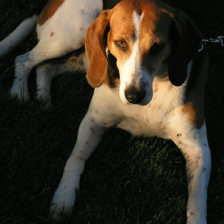
\includegraphics[width =
        .35\linewidth]{../repos/cockpit-paper/tex/fig/06_preprocessing/fig_samples/imagenetraw_vgg16_sample_00.png}}
      \Cshadowbox{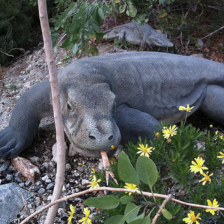
\includegraphics[width =
        .35\linewidth]{../repos/cockpit-paper/tex/fig/06_preprocessing/fig_samples/imagenetraw_vgg16_sample_01.png}}

      \Cshadowbox{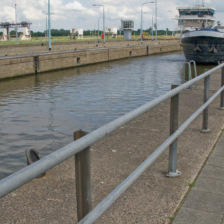
\includegraphics[width =
        .35\linewidth]{../repos/cockpit-paper/tex/fig/06_preprocessing/fig_samples/imagenetraw_vgg16_sample_02.png}}
      \Cshadowbox{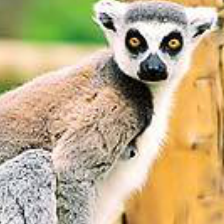
\includegraphics[width =
        .35\linewidth]{../repos/cockpit-paper/tex/fig/06_preprocessing/fig_samples/imagenetraw_vgg16_sample_03.png}}
    \end{minipage}
    \begin{minipage}{.49\linewidth}
      \pgfkeys{/pgfplots/preprocessingexperimentdefault/.style={
    width=1.15\linewidth,
    height=1.22\linewidth,
    every axis plot/.append style={line width = 1.5pt},
    tick pos = left,
    xmajorticks = true,
    ymajorticks = true,
    ylabel near ticks,
    xlabel near ticks,
    xtick align = inside,
    ytick align = inside,
    legend cell align = left,
    legend columns = 1,
    legend pos = south east,
    legend style = {
      fill opacity = 0.7,
      text opacity = 1,
      font = \footnotesize,
    },
    xticklabel style = {font = \footnotesize, inner xsep = 0ex},
    xlabel style = {font = \footnotesize},
    axis line style = {black},
    yticklabel style = {font = \footnotesize, inner ysep = -4ex},
    ylabel style = {font = \footnotesize},
    title style = {font = \footnotesize, inner ysep = -3ex},
    grid = major,
    grid style = {dashed}
  }
}
%%% Local Variables:
%%% mode: latex
%%% TeX-master: "../../../thesis"
%%% End:

      \centering
      % customize "zmystyle" as you wish
      \pgfkeys{/pgfplots/zmystyle/.style={preprocessingexperimentdefault,
          ylabel={Gradient Element}
        }}
      \vspace{1.4\baselineskip}
      \tikzexternalenable
      % This file was created with tikzplotlib v0.9.14.
\begin{tikzpicture}

\definecolor{color0}{rgb}{0.12156862745098,0.466666666666667,0.705882352941177}

\begin{axis}[
axis line style={white},
log basis x={10},
tick align=outside,
xmajorticks=false,
xmin=0.9, xmax=315917612.324796,
xmode=log,
xtick style={color=white!15!black},
ymajorticks=false,
ymin=-1.5, ymax=1.5,
zmystyle
]
\draw[draw=white,fill=color0,line width=0.04pt] (axis cs:0.9,-1.5) rectangle (axis cs:0.9,-1.42499995231628);
\draw[draw=white,fill=color0,line width=0.04pt] (axis cs:0.9,-1.42500007152557) rectangle (axis cs:0.9,-1.35000002384186);
\draw[draw=white,fill=color0,line width=0.04pt] (axis cs:0.9,-1.35000002384186) rectangle (axis cs:0.9,-1.27499997615814);
\draw[draw=white,fill=color0,line width=0.04pt] (axis cs:0.9,-1.27499997615814) rectangle (axis cs:0.9,-1.19999992847443);
\draw[draw=white,fill=color0,line width=0.04pt] (axis cs:0.9,-1.20000004768372) rectangle (axis cs:0.9,-1.125);
\draw[draw=white,fill=color0,line width=0.04pt] (axis cs:0.9,-1.125) rectangle (axis cs:0.9,-1.04999995231628);
\draw[draw=white,fill=color0,line width=0.04pt] (axis cs:0.9,-1.04999995231628) rectangle (axis cs:0.9,-0.974999904632568);
\draw[draw=white,fill=color0,line width=0.04pt] (axis cs:0.9,-0.975000023841858) rectangle (axis cs:0.9,-0.899999976158142);
\draw[draw=white,fill=color0,line width=0.04pt] (axis cs:0.9,-0.899999976158142) rectangle (axis cs:0.9,-0.824999928474426);
\draw[draw=white,fill=color0,line width=0.04pt] (axis cs:0.9,-0.825000047683716) rectangle (axis cs:0.9,-0.75);
\draw[draw=white,fill=color0,line width=0.04pt] (axis cs:0.9,-0.75) rectangle (axis cs:0.9,-0.674999952316284);
\draw[draw=white,fill=color0,line width=0.04pt] (axis cs:0.9,-0.674999952316284) rectangle (axis cs:0.9,-0.599999904632568);
\draw[draw=white,fill=color0,line width=0.04pt] (axis cs:0.9,-0.600000023841858) rectangle (axis cs:0.9,-0.524999976158142);
\draw[draw=white,fill=color0,line width=0.04pt] (axis cs:0.9,-0.524999976158142) rectangle (axis cs:0.9,-0.449999928474426);
\draw[draw=white,fill=color0,line width=0.04pt] (axis cs:0.9,-0.449999988079071) rectangle (axis cs:0.9,-0.374999940395355);
\draw[draw=white,fill=color0,line width=0.04pt] (axis cs:0.9,-0.374999970197678) rectangle (axis cs:0.9,-0.299999922513962);
\draw[draw=white,fill=color0,line width=0.04pt] (axis cs:0.9,-0.299999982118607) rectangle (axis cs:0.9,-0.224999934434891);
\draw[draw=white,fill=color0,line width=0.04pt] (axis cs:0.9,-0.224999964237213) rectangle (axis cs:3.9,-0.149999916553497);
\draw[draw=white,fill=color0,line width=0.04pt] (axis cs:0.9,-0.149999968707561) rectangle (axis cs:102.9,-0.0749999210238457);
\draw[draw=white,fill=color0,line width=0.04pt] (axis cs:0.9,-0.075000025331974) rectangle (axis cs:123780803.9,2.23517417907715e-08);
\draw[draw=white,fill=color0,line width=0.04pt] (axis cs:0.9,-8.19563865661621e-08) rectangle (axis cs:14580628.9,0.0749999657273293);
\draw[draw=white,fill=color0,line width=0.04pt] (axis cs:0.9,0.0749999210238457) rectangle (axis cs:98.9,0.149999968707561);
\draw[draw=white,fill=color0,line width=0.04pt] (axis cs:0.9,0.149999916553497) rectangle (axis cs:6.9,0.224999964237213);
\draw[draw=white,fill=color0,line width=0.04pt] (axis cs:0.9,0.224999934434891) rectangle (axis cs:0.9,0.299999982118607);
\draw[draw=white,fill=color0,line width=0.04pt] (axis cs:0.9,0.299999922513962) rectangle (axis cs:0.9,0.374999970197678);
\draw[draw=white,fill=color0,line width=0.04pt] (axis cs:0.9,0.374999940395355) rectangle (axis cs:0.9,0.449999988079071);
\draw[draw=white,fill=color0,line width=0.04pt] (axis cs:0.9,0.449999928474426) rectangle (axis cs:0.9,0.524999976158142);
\draw[draw=white,fill=color0,line width=0.04pt] (axis cs:0.9,0.524999976158142) rectangle (axis cs:0.9,0.600000023841858);
\draw[draw=white,fill=color0,line width=0.04pt] (axis cs:0.9,0.599999904632568) rectangle (axis cs:0.9,0.674999952316284);
\draw[draw=white,fill=color0,line width=0.04pt] (axis cs:0.9,0.674999952316284) rectangle (axis cs:0.9,0.75);
\draw[draw=white,fill=color0,line width=0.04pt] (axis cs:0.9,0.75) rectangle (axis cs:0.9,0.825000047683716);
\draw[draw=white,fill=color0,line width=0.04pt] (axis cs:0.9,0.824999928474426) rectangle (axis cs:0.9,0.899999976158142);
\draw[draw=white,fill=color0,line width=0.04pt] (axis cs:0.9,0.899999976158142) rectangle (axis cs:0.9,0.975000023841858);
\draw[draw=white,fill=color0,line width=0.04pt] (axis cs:0.9,0.974999904632568) rectangle (axis cs:1.9,1.04999995231628);
\draw[draw=white,fill=color0,line width=0.04pt] (axis cs:0.9,1.04999995231628) rectangle (axis cs:0.9,1.125);
\draw[draw=white,fill=color0,line width=0.04pt] (axis cs:0.9,1.125) rectangle (axis cs:0.9,1.20000004768372);
\draw[draw=white,fill=color0,line width=0.04pt] (axis cs:0.9,1.19999992847443) rectangle (axis cs:0.9,1.27499997615814);
\draw[draw=white,fill=color0,line width=0.04pt] (axis cs:0.9,1.27499997615814) rectangle (axis cs:0.9,1.35000002384186);
\draw[draw=white,fill=color0,line width=0.04pt] (axis cs:0.9,1.35000002384186) rectangle (axis cs:0.9,1.42500007152557);
\draw[draw=white,fill=color0,line width=0.04pt] (axis cs:0.9,1.42499995231628) rectangle (axis cs:0.9,1.5);
\end{axis}

\end{tikzpicture}

      \tikzexternaldisable
    \end{minipage}
    \vspace{-2ex}
    \caption{Normalized Data}
    \label{cockpit::fig:data-pre-processing_norm_imagenet}
  \end{subfigure}
  \hfill
  \begin{subfigure}[t]{0.46\linewidth}
    \begin{minipage}{.49\linewidth}
      \Cshadowbox{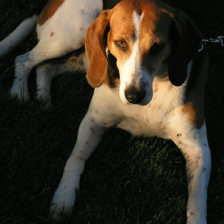
\includegraphics[width =
        .35\linewidth]{../repos/cockpit-paper/tex/fig/06_preprocessing/fig_samples/imagenetscale255_vgg16_sample_00.png}}
      \Cshadowbox{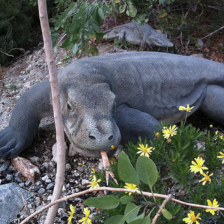
\includegraphics[width =
        .35\linewidth]{../repos/cockpit-paper/tex/fig/06_preprocessing/fig_samples/imagenetscale255_vgg16_sample_01.png}}

      \Cshadowbox{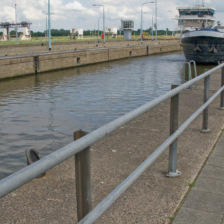
\includegraphics[width =
        .35\linewidth]{../repos/cockpit-paper/tex/fig/06_preprocessing/fig_samples/imagenetscale255_vgg16_sample_02.png}}
      \Cshadowbox{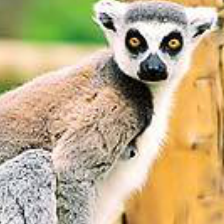
\includegraphics[width =
        .35\linewidth]{../repos/cockpit-paper/tex/fig/06_preprocessing/fig_samples/imagenetscale255_vgg16_sample_03.png}}
    \end{minipage}
    \begin{minipage}{.49\linewidth}
      \centering
      \pgfkeys{/pgfplots/preprocessingexperimentdefault/.style={
    width=1.15\linewidth,
    height=1.22\linewidth,
    every axis plot/.append style={line width = 1.5pt},
    tick pos = left,
    xmajorticks = true,
    ymajorticks = true,
    ylabel near ticks,
    xlabel near ticks,
    xtick align = inside,
    ytick align = inside,
    legend cell align = left,
    legend columns = 1,
    legend pos = south east,
    legend style = {
      fill opacity = 0.7,
      text opacity = 1,
      font = \footnotesize,
    },
    xticklabel style = {font = \footnotesize, inner xsep = 0ex},
    xlabel style = {font = \footnotesize},
    axis line style = {black},
    yticklabel style = {font = \footnotesize, inner ysep = -4ex},
    ylabel style = {font = \footnotesize},
    title style = {font = \footnotesize, inner ysep = -3ex},
    grid = major,
    grid style = {dashed}
  }
}
%%% Local Variables:
%%% mode: latex
%%% TeX-master: "../../../thesis"
%%% End:

      % customize "zmystyle" as you wish
      \pgfkeys{/pgfplots/zmystyle/.style={preprocessingexperimentdefault,
          ylabel={Gradient Element}
        }}
      \vspace{1.4\baselineskip}
      \tikzexternalenable
      % This file was created with tikzplotlib v0.9.14.
\begin{tikzpicture}

\definecolor{color0}{rgb}{1,0.498039215686275,0.0549019607843137}

\begin{axis}[
axis line style={white},
log basis x={10},
tick align=outside,
xmajorticks=false,
xmin=0.9, xmax=315354991.80789,
xmode=log,
xtick style={color=white!15!black},
ymajorticks=false,
ymin=-1.5, ymax=1.5,
zmystyle
]
\draw[draw=white,fill=color0,line width=0.04pt] (axis cs:0.9,-1.5) rectangle (axis cs:0.9,-1.42499995231628);
\draw[draw=white,fill=color0,line width=0.04pt] (axis cs:0.9,-1.42500007152557) rectangle (axis cs:0.9,-1.35000002384186);
\draw[draw=white,fill=color0,line width=0.04pt] (axis cs:0.9,-1.35000002384186) rectangle (axis cs:0.9,-1.27499997615814);
\draw[draw=white,fill=color0,line width=0.04pt] (axis cs:0.9,-1.27499997615814) rectangle (axis cs:0.9,-1.19999992847443);
\draw[draw=white,fill=color0,line width=0.04pt] (axis cs:0.9,-1.20000004768372) rectangle (axis cs:0.9,-1.125);
\draw[draw=white,fill=color0,line width=0.04pt] (axis cs:0.9,-1.125) rectangle (axis cs:0.9,-1.04999995231628);
\draw[draw=white,fill=color0,line width=0.04pt] (axis cs:0.9,-1.04999995231628) rectangle (axis cs:0.9,-0.974999904632568);
\draw[draw=white,fill=color0,line width=0.04pt] (axis cs:0.9,-0.975000023841858) rectangle (axis cs:0.9,-0.899999976158142);
\draw[draw=white,fill=color0,line width=0.04pt] (axis cs:0.9,-0.899999976158142) rectangle (axis cs:0.9,-0.824999928474426);
\draw[draw=white,fill=color0,line width=0.04pt] (axis cs:0.9,-0.825000047683716) rectangle (axis cs:0.9,-0.75);
\draw[draw=white,fill=color0,line width=0.04pt] (axis cs:0.9,-0.75) rectangle (axis cs:0.9,-0.674999952316284);
\draw[draw=white,fill=color0,line width=0.04pt] (axis cs:0.9,-0.674999952316284) rectangle (axis cs:0.9,-0.599999904632568);
\draw[draw=white,fill=color0,line width=0.04pt] (axis cs:0.9,-0.600000023841858) rectangle (axis cs:0.9,-0.524999976158142);
\draw[draw=white,fill=color0,line width=0.04pt] (axis cs:0.9,-0.524999976158142) rectangle (axis cs:0.9,-0.449999928474426);
\draw[draw=white,fill=color0,line width=0.04pt] (axis cs:0.9,-0.449999988079071) rectangle (axis cs:0.9,-0.374999940395355);
\draw[draw=white,fill=color0,line width=0.04pt] (axis cs:0.9,-0.374999970197678) rectangle (axis cs:0.9,-0.299999922513962);
\draw[draw=white,fill=color0,line width=0.04pt] (axis cs:0.9,-0.299999982118607) rectangle (axis cs:40.9,-0.224999934434891);
\draw[draw=white,fill=color0,line width=0.04pt] (axis cs:0.9,-0.224999964237213) rectangle (axis cs:872.9,-0.149999916553497);
\draw[draw=white,fill=color0,line width=0.04pt] (axis cs:0.9,-0.149999968707561) rectangle (axis cs:45198.9,-0.0749999210238457);
\draw[draw=white,fill=color0,line width=0.04pt] (axis cs:0.9,-0.075000025331974) rectangle (axis cs:123570849.9,2.23517417907715e-08);
\draw[draw=white,fill=color0,line width=0.04pt] (axis cs:0.9,-8.19563865661621e-08) rectangle (axis cs:14693460.9,0.0749999657273293);
\draw[draw=white,fill=color0,line width=0.04pt] (axis cs:0.9,0.0749999210238457) rectangle (axis cs:48872.9,0.149999968707561);
\draw[draw=white,fill=color0,line width=0.04pt] (axis cs:0.9,0.149999916553497) rectangle (axis cs:1580.9,0.224999964237213);
\draw[draw=white,fill=color0,line width=0.04pt] (axis cs:0.9,0.224999934434891) rectangle (axis cs:137.9,0.299999982118607);
\draw[draw=white,fill=color0,line width=0.04pt] (axis cs:0.9,0.299999922513962) rectangle (axis cs:91.9,0.374999970197678);
\draw[draw=white,fill=color0,line width=0.04pt] (axis cs:0.9,0.374999940395355) rectangle (axis cs:74.9,0.449999988079071);
\draw[draw=white,fill=color0,line width=0.04pt] (axis cs:0.9,0.449999928474426) rectangle (axis cs:73.9,0.524999976158142);
\draw[draw=white,fill=color0,line width=0.04pt] (axis cs:0.9,0.524999976158142) rectangle (axis cs:62.9,0.600000023841858);
\draw[draw=white,fill=color0,line width=0.04pt] (axis cs:0.9,0.599999904632568) rectangle (axis cs:44.9,0.674999952316284);
\draw[draw=white,fill=color0,line width=0.04pt] (axis cs:0.9,0.674999952316284) rectangle (axis cs:58.9,0.75);
\draw[draw=white,fill=color0,line width=0.04pt] (axis cs:0.9,0.75) rectangle (axis cs:54.9,0.825000047683716);
\draw[draw=white,fill=color0,line width=0.04pt] (axis cs:0.9,0.824999928474426) rectangle (axis cs:45.9,0.899999976158142);
\draw[draw=white,fill=color0,line width=0.04pt] (axis cs:0.9,0.899999976158142) rectangle (axis cs:27.9,0.975000023841858);
\draw[draw=white,fill=color0,line width=0.04pt] (axis cs:0.9,0.974999904632568) rectangle (axis cs:21.9,1.04999995231628);
\draw[draw=white,fill=color0,line width=0.04pt] (axis cs:0.9,1.04999995231628) rectangle (axis cs:23.9,1.125);
\draw[draw=white,fill=color0,line width=0.04pt] (axis cs:0.9,1.125) rectangle (axis cs:12.9,1.20000004768372);
\draw[draw=white,fill=color0,line width=0.04pt] (axis cs:0.9,1.19999992847443) rectangle (axis cs:11.9,1.27499997615814);
\draw[draw=white,fill=color0,line width=0.04pt] (axis cs:0.9,1.27499997615814) rectangle (axis cs:12.9,1.35000002384186);
\draw[draw=white,fill=color0,line width=0.04pt] (axis cs:0.9,1.35000002384186) rectangle (axis cs:6.9,1.42500007152557);
\draw[draw=white,fill=color0,line width=0.04pt] (axis cs:0.9,1.42499995231628) rectangle (axis cs:20.9,1.5);
\end{axis}

\end{tikzpicture}

      \tikzexternaldisable
    \end{minipage}
    \vspace{-2ex}
    \caption{Raw Data}
    \label{cockpit::fig:data-pre-processing_raw_imagenet}
  \end{subfigure}
  \caption{\textbf{Same inputs, different gradients on ImageNet.} This is
    structurally the same plot as \Cref{cockpit::fig:data-pre-processing}, but
    using \imagenet and \vgg.
    \subfigref{cockpit::fig:data-pre-processing_norm_imagenet} \emph{normalized}
    ($[0, 1]$) and \subfigref{cockpit::fig:data-pre-processing_raw_imagenet}
    \emph{raw} $([0, 255])$ images look identical in auto-scaled front-ends like
    \matplotlib's \robustInlinecode{imshow}. The gradient distribution on the \vgg model,
    however, is affected by this scaling.}
  \label{cockpit::fig:data-pre-processing_imagenet}
\end{figure*}

%%% Local Variables:
%%% mode: latex
%%% TeX-master: "../../../thesis"
%%% End:


%%% Local Variables:
%%% mode: latex
%%% TeX-master: "../thesis"
%%% End:

\subsection{Detecting Implicit Regularization of The
  Optimizer}\label{cockpit::app:implicit_regularization_exp}

In non-convex optimization, optimizers can converge to local minima with
different properties. Here, we illustrate this by investigating the effect of
sub-sampling noise on a simple task from
\cite{mulayoff2020unique,ginsburg2020regularization}.

We generate synthetic data $\sD = \{(x_n, y_n) \in \sR \times \sR
\}_{n=1}^{N=100}$ for a regression task with $x \sim \gN(\giventhat{x}{0, 1})$
with noisy observations $y = 1.4 x + \epsilon$ where $\epsilon \sim
\gN(\giventhat{\epsilon}{0,1})$. The model is a scalar net with parameters
$\vtheta = \begin{pmatrix} w_1 & w_2 \end{pmatrix}^\top \in \sR^2$, initialized
at $\vtheta_0 = \begin{pmatrix} 0.1 & 1.7 \end{pmatrix}^\top$, that produces
predictions $f_{\vtheta}(x) = w_2 w_1 x$. We seek to minimize the mean squared
error
\begin{equation*}
  \gL_\sD(\vtheta) = \frac{1}{N} \sum_{n=1}^{N} \left( f_{\vtheta}(x_n) - y_n \right)^2
\end{equation*}
and compare \sgd ($|\sB|=95$) with \gd ($|\sB|= N =100$) at a learning rate of
$0.1$ (see \Cref{cockpit::fig:implicit-regularization}).

We observe that the loss of both \sgd and \gd is almost identical. Using a noisy
gradient regularizes the Hessian's maximum eigenvalue though. It decreases in
later stages where the loss curve suggests that training has converged. This
regularization effect constitutes an important phenomenon that cannot be
observed by monitoring only the loss.

\pgfkeys{/pgfplots/regularizationdefault/.style={
    width=1.05\linewidth,
    height=0.8\linewidth,
    every axis plot/.append style={line width = 1.5pt},
    every axis background/.style={fill=white},
    ymajorticks=true,
    xmajorticks=true,
    tick pos = left,
    ylabel near ticks,
    xlabel near ticks,
    xtick align = inside,
    ytick align = inside,
    legend cell align = left,
    legend columns = 1,
    legend pos = north east,
    legend style = {
      fill opacity = 0.7,
      text opacity = 1,
      font = \footnotesize,
    },
    colorbar style = {font = \footnotesize},
    title style = {font = \footnotesize, inner ysep = 0ex},
    xticklabel style = {font = \footnotesize, inner xsep = 0ex},
    xlabel style = {font = \footnotesize},
    axis line style = {black},
    yticklabel style = {font = \footnotesize, inner ysep = -4ex},
    ylabel style = {font = \footnotesize},
    grid = major,
    grid style = {dashed}
  }
}

\begin{figure}[!th]
  \centering
	\begin{subfigure}[t]{0.495\textwidth}
    \centering
		\pgfkeys{/pgfplots/zmystyle/.style={regularizationdefault, ymin=0.6, ymax=1.1}}
    \tikzexternalenable
		% This file was created by tikzplotlib v0.9.7.
\begin{tikzpicture}

\definecolor{color0}{rgb}{0.12156862745098,0.466666666666667,0.705882352941177}
\definecolor{color1}{rgb}{1,0.498039215686275,0.0549019607843137}

\begin{axis}[
axis line style={white},
legend style={fill opacity=0.8, draw opacity=1, text opacity=1, draw=white!80!black},
log basis x={10},
tick align=outside,
xlabel={Iteration},
xmajorticks=false,
xmin=0.563970595937194, xmax=167345.603972783,
xmode=log,
xtick style={color=white!15!black},
ylabel={Mini-Batch Loss},
ymajorticks=false,
ymin=0.614918631315231, ymax=1.72726913094521,
zmystyle
]
\addplot [, color0]
table {%
0 1.65519058704376
1 1.01682019233704
2 0.780193150043488
3 0.775982201099396
4 0.737731337547302
5 0.771629452705383
6 0.738641858100891
7 0.745266854763031
8 0.772922933101654
9 0.748066663742065
10 0.77786260843277
11 0.769368886947632
12 0.775993466377258
13 0.769854426383972
14 0.780099034309387
15 0.732372939586639
16 0.76972508430481
17 0.77314555644989
18 0.787652790546417
19 0.731954038143158
20 0.753742933273315
21 0.760406374931335
22 0.772047460079193
24 0.752689599990845
25 0.768256425857544
27 0.772502541542053
28 0.745130240917206
30 0.73753297328949
32 0.775065541267395
34 0.7575803399086
36 0.748904526233673
38 0.78914475440979
40 0.774977564811707
42 0.770744025707245
45 0.771463930606842
48 0.724553644657135
51 0.750621318817139
54 0.786653280258179
57 0.740645587444305
60 0.780794203281403
64 0.765990436077118
68 0.772936582565308
72 0.764917433261871
76 0.75068473815918
81 0.763052582740784
86 0.766409575939178
91 0.779118478298187
96 0.779287576675415
102 0.694868266582489
108 0.753131628036499
114 0.745236694812775
121 0.769624173641205
128 0.733922481536865
136 0.763625741004944
144 0.771767735481262
153 0.778103351593018
162 0.76782751083374
172 0.770959913730621
182 0.778098523616791
193 0.747863173484802
204 0.767393231391907
217 0.747031450271606
230 0.761284053325653
243 0.788995981216431
258 0.78480863571167
273 0.725325763225555
289 0.788911044597626
307 0.757820010185242
325 0.701482534408569
344 0.786840677261353
365 0.75093948841095
387 0.793320834636688
410 0.733399331569672
434 0.790173828601837
460 0.789791882038116
488 0.772913932800293
517 0.747723639011383
547 0.767966389656067
580 0.769767463207245
615 0.777678191661835
651 0.732484042644501
690 0.765304982662201
731 0.779313802719116
775 0.752284646034241
821 0.751649916172028
870 0.763818562030792
922 0.763033270835876
977 0.76042252779007
1035 0.794110774993896
1096 0.770817458629608
1162 0.719465613365173
1231 0.773622274398804
1304 0.777041494846344
1382 0.752636194229126
1464 0.746034681797028
1552 0.756577551364899
1644 0.710349500179291
1742 0.788471639156342
1846 0.749858379364014
1956 0.751055300235748
2072 0.77653980255127
2196 0.743179202079773
2327 0.777839779853821
2465 0.765402734279633
2612 0.784416019916534
2768 0.675363481044769
2933 0.767980337142944
3107 0.77206939458847
3292 0.761081337928772
3489 0.780567407608032
3696 0.759546518325806
3917 0.772010743618011
4150 0.731160163879395
4397 0.778384268283844
4659 0.792823255062103
4937 0.780224800109863
5231 0.716187834739685
5542 0.732295513153076
5872 0.757798075675964
6222 0.783280313014984
6593 0.774591028690338
6985 0.76332038640976
7401 0.73084568977356
7842 0.744604051113129
8309 0.77698802947998
8804 0.770139813423157
9329 0.7605100274086
9884 0.745865881443024
10473 0.772988736629486
11097 0.784264206886292
11758 0.73901504278183
12458 0.665480017662048
13200 0.74626225233078
13987 0.765305399894714
14820 0.788454294204712
15702 0.783531785011292
16638 0.790920555591583
17629 0.723659753799438
18679 0.79127299785614
19791 0.776141047477722
20970 0.772833287715912
22219 0.73369562625885
23542 0.771220922470093
24945 0.785363912582397
26430 0.72164660692215
28005 0.788875877857208
29673 0.772274553775787
31440 0.764169812202454
33312 0.723604738712311
35297 0.758412897586823
37399 0.769568562507629
39626 0.782877564430237
41987 0.774317562580109
44487 0.74730920791626
47137 0.759216368198395
49945 0.75877833366394
52919 0.77678370475769
56071 0.770803034305573
59411 0.757794678211212
62949 0.775205314159393
66699 0.787786245346069
70671 0.761527419090271
74881 0.740764439105988
79340 0.766364872455597
84066 0.771571159362793
89073 0.774646580219269
94378 0.766631364822388
};
\addlegendentry{SGD}
\addplot [, color1]
table {%
0 1.67670774459839
1 1.00288474559784
2 0.814482688903809
3 0.769742786884308
4 0.761073589324951
5 0.759601593017578
6 0.759367525577545
7 0.759331345558167
8 0.759325861930847
9 0.759325087070465
10 0.759324848651886
11 0.759324848651886
12 0.759324908256531
13 0.759324848651886
14 0.759324848651886
15 0.759324848651886
16 0.759324848651886
17 0.759324848651886
18 0.759324908256531
19 0.759324848651886
20 0.759324848651886
21 0.759324848651886
22 0.759324848651886
24 0.759324789047241
25 0.759324848651886
27 0.759324848651886
28 0.759324848651886
30 0.759324848651886
32 0.759324848651886
34 0.759324848651886
36 0.759324908256531
38 0.759324848651886
40 0.759324848651886
42 0.759324848651886
45 0.759324908256531
48 0.759324848651886
51 0.759324848651886
54 0.759324848651886
57 0.759324848651886
60 0.759324848651886
64 0.759324848651886
68 0.759324848651886
72 0.759324848651886
76 0.759324848651886
81 0.759324908256531
86 0.759324789047241
91 0.759324848651886
96 0.759324908256531
102 0.759324848651886
108 0.759324848651886
114 0.759324908256531
121 0.759324848651886
128 0.759324848651886
136 0.759324789047241
144 0.759324908256531
153 0.759324848651886
162 0.759324848651886
172 0.759324908256531
182 0.759324908256531
193 0.759324848651886
204 0.759324908256531
217 0.759324908256531
230 0.759324908256531
243 0.759324848651886
258 0.759324848651886
273 0.759324908256531
289 0.759324848651886
307 0.759324848651886
325 0.759324848651886
344 0.759324789047241
365 0.759324848651886
387 0.759324848651886
410 0.759324908256531
434 0.759324848651886
460 0.759324848651886
488 0.759324848651886
517 0.759324848651886
547 0.759324848651886
580 0.759324908256531
615 0.759324908256531
651 0.759324848651886
690 0.759324848651886
731 0.759324848651886
775 0.759324789047241
821 0.759324848651886
870 0.759324848651886
922 0.759324848651886
977 0.759324848651886
1035 0.759324908256531
1096 0.759324908256531
1162 0.759324789047241
1231 0.759324848651886
1304 0.759324848651886
1382 0.759324848651886
1464 0.759324848651886
1552 0.759324848651886
1644 0.759324848651886
1742 0.759324908256531
1846 0.759324848651886
1956 0.759324908256531
2072 0.759324908256531
2196 0.759324908256531
2327 0.759324789047241
2465 0.759324908256531
2612 0.759324848651886
2768 0.759324848651886
2933 0.759324848651886
3107 0.759324848651886
3292 0.759324908256531
3489 0.759324908256531
3696 0.759324908256531
3917 0.759324848651886
4150 0.759324848651886
4397 0.759324848651886
4659 0.759324848651886
4937 0.759324848651886
5231 0.759324848651886
5542 0.759324848651886
5872 0.759324908256531
6222 0.759324908256531
6593 0.759324848651886
6985 0.759324908256531
7401 0.759324908256531
7842 0.759324848651886
8309 0.759324848651886
8804 0.759324908256531
9329 0.759324848651886
9884 0.759324908256531
10473 0.759324848651886
11097 0.759324908256531
11758 0.759324848651886
12458 0.759324848651886
13200 0.759324848651886
13987 0.759324908256531
14820 0.759324908256531
15702 0.759324848651886
16638 0.759324848651886
17629 0.759324848651886
18679 0.759324908256531
19791 0.759324908256531
20970 0.759324848651886
22219 0.759324848651886
23542 0.759324848651886
24945 0.759324848651886
26430 0.759324908256531
28005 0.759324848651886
29673 0.759324848651886
31440 0.759324789047241
33312 0.759324848651886
35297 0.759324848651886
37399 0.759324789047241
39626 0.759324908256531
41987 0.759324848651886
44487 0.759324848651886
47137 0.759324848651886
49945 0.759324848651886
52919 0.759324848651886
56071 0.759324848651886
59411 0.759324908256531
62949 0.759324789047241
66699 0.759324848651886
70671 0.759324848651886
74881 0.759324848651886
79340 0.759324848651886
84066 0.759324848651886
89073 0.759324848651886
94378 0.759324908256531
};
\addlegendentry{GD}
\end{axis}

\end{tikzpicture}

    \tikzexternaldisable
	\end{subfigure}
	\hfill
	\begin{subfigure}[t]{0.495\textwidth}
    \centering
		\pgfkeys{/pgfplots/zmystyle/.style={regularizationdefault,
        legend style = {
          opacity = 0,
          fill opacity = 0,
          text opacity = 0,
        },
        ylabel = {Max.\,Hessian eigenvalue}
      }}
    \tikzexternalenable
		% This file was created by tikzplotlib v0.9.7.
\begin{tikzpicture}

\definecolor{color0}{rgb}{0.12156862745098,0.466666666666667,0.705882352941177}
\definecolor{color1}{rgb}{1,0.498039215686275,0.0549019607843137}

\begin{axis}[
axis line style={white},
legend style={fill opacity=0.8, draw opacity=1, text opacity=1, draw=white!80!black},
log basis x={10},
tick align=outside,
xlabel={Iteration},
xmajorticks=false,
xmin=0.563970595937194, xmax=167345.603972783,
xmode=log,
xtick style={color=white!15!black},
ylabel={Maximum Hessian eigenvalue},
ymajorticks=false,
ymin=3.85510742664337, ymax=6.68519914150238,
zmystyle
]
\addplot [, color0]
table {%
0 5.01858520507812
1 4.91631031036377
2 5.16143560409546
3 5.60115337371826
4 5.79127502441406
5 6.0561056137085
6 6.26061916351318
7 6.19245529174805
8 6.1329493522644
9 6.05357074737549
10 5.97355842590332
11 6.05519437789917
12 6.31369209289551
13 6.22404289245605
14 6.33904695510864
15 5.68460321426392
16 6.16733026504517
17 6.17319679260254
18 6.14776849746704
19 6.2695107460022
20 6.03493785858154
21 6.15226316452026
22 6.19907712936401
24 5.59337615966797
25 6.36163806915283
27 6.35177993774414
28 6.22747230529785
30 5.91255331039429
32 6.19828081130981
34 6.39521312713623
36 6.0371265411377
38 6.43193244934082
40 6.14503479003906
42 6.25523281097412
45 6.05292510986328
48 5.67981719970703
51 6.36472225189209
54 6.06869220733643
57 6.18863964080811
60 5.93778562545776
64 6.12580823898315
68 6.18363857269287
72 6.01109552383423
76 6.02523136138916
81 6.21799850463867
86 6.18191480636597
91 6.55655860900879
96 6.31975746154785
102 6.05267763137817
108 6.0778636932373
114 6.01467657089233
121 6.24698925018311
128 6.04640293121338
136 6.24112749099731
144 6.31688690185547
153 6.28657817840576
162 6.13792037963867
172 5.65208387374878
182 6.30600261688232
193 5.98742771148682
204 5.71659326553345
217 5.84029388427734
230 6.0068564414978
243 6.3081259727478
258 6.39043521881104
273 6.14346885681152
289 6.18961191177368
307 6.13053369522095
325 6.17688846588135
344 5.90940189361572
365 5.89127063751221
387 5.98564434051514
410 6.25674438476562
434 5.93166160583496
460 6.01510143280029
488 6.29282379150391
517 6.3133373260498
547 5.89875364303589
580 5.78323602676392
615 6.22842979431152
651 6.12653160095215
690 6.13379669189453
731 6.08839702606201
775 6.19680023193359
821 6.05588006973267
870 6.21298170089722
922 6.0586724281311
977 5.70560264587402
1035 6.05281639099121
1096 6.12884950637817
1162 5.72979116439819
1231 5.75020885467529
1304 5.78489637374878
1382 6.24677515029907
1464 5.72618103027344
1552 6.16928005218506
1644 5.99916076660156
1742 6.31236791610718
1846 5.42526912689209
1956 6.01460218429565
2072 6.17887306213379
2196 5.93650770187378
2327 6.21088695526123
2465 5.92963600158691
2612 5.98927402496338
2768 6.04936790466309
2933 5.9457950592041
3107 6.15447568893433
3292 6.04442024230957
3489 5.88113212585449
3696 6.0181360244751
3917 5.82596063613892
4150 5.97462749481201
4397 5.84421348571777
4659 5.84129619598389
4937 5.80539751052856
5231 6.00247669219971
5542 5.8760838508606
5872 5.92244338989258
6222 5.69848346710205
6593 5.64358997344971
6985 5.6120719909668
7401 5.73087453842163
7842 5.67744302749634
8309 5.43394136428833
8804 5.7706823348999
9329 5.68305492401123
9884 5.22680282592773
10473 5.09199523925781
11097 5.7391529083252
11758 5.49506330490112
12458 5.29003858566284
13200 5.21850109100342
13987 5.15451717376709
14820 5.25626420974731
15702 5.2664647102356
16638 5.09290647506714
17629 5.06191682815552
18679 5.22023582458496
19791 4.99110126495361
20970 5.13607454299927
22219 4.82361221313477
23542 4.96726989746094
24945 4.517502784729
26430 4.89909362792969
28005 4.69721984863281
29673 4.44070720672607
31440 4.71606779098511
33312 4.43321752548218
35297 4.52913951873779
37399 4.35525035858154
39626 4.48494052886963
41987 4.43455600738525
44487 4.4298300743103
47137 4.41794347763062
49945 4.16174602508545
52919 4.41815376281738
56071 4.30182790756226
59411 4.18179321289062
62949 4.38689374923706
66699 4.22925329208374
70671 4.26896953582764
74881 4.2410717010498
79340 4.02750778198242
84066 3.98374795913696
89073 4.10416793823242
94378 4.25959587097168
};
\addlegendentry{SGD}
\addplot [, color1]
table {%
0 5.19412231445312
1 4.89158582687378
2 5.36561346054077
3 5.75625705718994
4 5.95861196517944
5 6.04718065261841
6 6.08332633972168
7 6.09766292572021
8 6.10328483581543
9 6.10547971725464
10 6.10633707046509
11 6.10666942596436
12 6.10679912567139
13 6.106849193573
14 6.10686922073364
15 6.10687732696533
16 6.10687875747681
17 6.1068811416626
18 6.1068811416626
19 6.10688161849976
20 6.10688161849976
21 6.10688161849976
22 6.10688161849976
24 6.10688161849976
25 6.1068811416626
27 6.10688209533691
28 6.1068811416626
30 6.10688161849976
32 6.10688161849976
34 6.10688161849976
36 6.10688161849976
38 6.10688161849976
40 6.1068811416626
42 6.10688161849976
45 6.10688161849976
48 6.10688257217407
51 6.10688209533691
54 6.10688161849976
57 6.10688209533691
60 6.10688161849976
64 6.10688209533691
68 6.1068811416626
72 6.10688161849976
76 6.10688161849976
81 6.10688257217407
86 6.10688161849976
91 6.1068811416626
96 6.10688209533691
102 6.10688257217407
108 6.10688161849976
114 6.10688209533691
121 6.1068811416626
128 6.10688257217407
136 6.10688161849976
144 6.10688209533691
153 6.10688161849976
162 6.10688209533691
172 6.10688161849976
182 6.10688161849976
193 6.1068811416626
204 6.10688161849976
217 6.10688257217407
230 6.1068811416626
243 6.10688209533691
258 6.1068811416626
273 6.1068811416626
289 6.10688161849976
307 6.10688161849976
325 6.1068811416626
344 6.10688161849976
365 6.10688161849976
387 6.10688161849976
410 6.10688209533691
434 6.10688161849976
460 6.10688161849976
488 6.1068811416626
517 6.10688161849976
547 6.10688161849976
580 6.10688209533691
615 6.10688161849976
651 6.1068811416626
690 6.1068811416626
731 6.1068811416626
775 6.1068811416626
821 6.1068811416626
870 6.10688209533691
922 6.10688161849976
977 6.10688161849976
1035 6.10688161849976
1096 6.10688161849976
1162 6.10688161849976
1231 6.1068811416626
1304 6.10688209533691
1382 6.10688161849976
1464 6.10688161849976
1552 6.1068811416626
1644 6.1068811416626
1742 6.10688161849976
1846 6.10688209533691
1956 6.10688161849976
2072 6.1068811416626
2196 6.10688161849976
2327 6.1068811416626
2465 6.10688161849976
2612 6.10688161849976
2768 6.10688161849976
2933 6.10688209533691
3107 6.10688257217407
3292 6.10688161849976
3489 6.10688257217407
3696 6.10688161849976
3917 6.1068811416626
4150 6.10688209533691
4397 6.1068811416626
4659 6.10688161849976
4937 6.10688209533691
5231 6.10688161849976
5542 6.1068811416626
5872 6.10688161849976
6222 6.10688209533691
6593 6.1068811416626
6985 6.10688161849976
7401 6.10688209533691
7842 6.10688161849976
8309 6.10688209533691
8804 6.10688161849976
9329 6.10688161849976
9884 6.1068811416626
10473 6.1068811416626
11097 6.10688161849976
11758 6.10688161849976
12458 6.10688161849976
13200 6.1068811416626
13987 6.1068811416626
14820 6.1068811416626
15702 6.10688161849976
16638 6.10688161849976
17629 6.10688161849976
18679 6.10688161849976
19791 6.1068811416626
20970 6.1068811416626
22219 6.1068811416626
23542 6.10688209533691
24945 6.10688161849976
26430 6.10688209533691
28005 6.10688209533691
29673 6.1068811416626
31440 6.10688161849976
33312 6.10688209533691
35297 6.10688161849976
37399 6.10688161849976
39626 6.10688209533691
41987 6.10688161849976
44487 6.10688161849976
47137 6.10688161849976
49945 6.1068811416626
52919 6.10688209533691
56071 6.10688209533691
59411 6.10688161849976
62949 6.10688161849976
66699 6.10688161849976
70671 6.10688161849976
74881 6.10688161849976
79340 6.10688161849976
84066 6.10688161849976
89073 6.1068811416626
94378 6.10688161849976
};
\addlegendentry{GD}
\end{axis}

\end{tikzpicture}

    \tikzexternaldisable
	\end{subfigure}
  \vspace{1ex}
  \begin{subfigure}{1.0\linewidth}
    \centering
		\pgfkeys{/pgfplots/zmystyle/.style={regularizationdefault,
        width = 0.91\linewidth,
        height = 0.6695*0.91*\linewidth,
        legend style = {
          opacity = 0,
          fill opacity = 0,
          text opacity = 0,
        },
        xmajorticks=true,
        ymajorticks=true,
      }}
    \tikzexternalenable
    % This file was created by tikzplotlib v0.9.7.
\begin{tikzpicture}

\definecolor{color0}{rgb}{0.12156862745098,0.466666666666667,0.705882352941177}
\definecolor{color1}{rgb}{1,0.498039215686275,0.0549019607843137}

\begin{axis}[
axis line style={white},
colorbar,
colormap={mymap}{[1pt]
  rgb(0pt)=(1,1,0.850980392156863);
  rgb(1pt)=(0.929411764705882,0.972549019607843,0.694117647058824);
  rgb(2pt)=(0.780392156862745,0.913725490196078,0.705882352941177);
  rgb(3pt)=(0.498039215686275,0.803921568627451,0.733333333333333);
  rgb(4pt)=(0.254901960784314,0.713725490196078,0.768627450980392);
  rgb(5pt)=(0.113725490196078,0.568627450980392,0.752941176470588);
  rgb(6pt)=(0.133333333333333,0.368627450980392,0.658823529411765);
  rgb(7pt)=(0.145098039215686,0.203921568627451,0.580392156862745);
  rgb(8pt)=(0.0313725490196078,0.113725490196078,0.345098039215686)
},
legend style={fill opacity=0.8, draw opacity=1, text opacity=1, draw=white!80!black},
point meta max=33.3554496765137,
point meta min=0.759324848651886,
tick align=outside,
title={Loss landscape},
xlabel={\(\displaystyle \theta_1\)},
xmajorticks=false,
xmin=-1, xmax=2.5,
xtick style={color=white!15!black},
ylabel={\(\displaystyle \theta_2\)},
ymajorticks=false,
ymin=-0.5, ymax=3,
zmystyle
]
\addplot graphics [,xmin=-1, xmax=2.5, ymin=-0.5, ymax=3] {Trajectory-000.png};
\addplot [, color0]
table {%
0.100000001490116 1.70000004768372
0.390511572360992 1.7170889377594
0.546473205089569 1.75255870819092
0.601417779922485 1.76969122886658
0.639493048191071 1.78263092041016
0.645879983901978 1.78492212295532
0.667922377586365 1.79289829730988
0.669110357761383 1.79334080219269
0.682194948196411 1.79822278022766
0.674466907978058 1.79529094696045
0.663153052330017 1.79104053974152
0.673606514930725 1.79491102695465
0.675003290176392 1.79543519020081
0.678699016571045 1.79682457447052
0.685095965862274 1.79924082756042
0.687204122543335 1.80004358291626
0.691844761371613 1.80181527137756
0.671525537967682 1.79401326179504
0.675070106983185 1.79534006118774
0.67482715845108 1.79524874687195
0.678539335727692 1.79664409160614
0.685560762882233 1.7992959022522
0.67389988899231 1.79485297203064
0.677536308765411 1.79621696472168
0.700529396533966 1.80489003658295
0.682436764240265 1.79790055751801
0.681613385677338 1.7975879907608
0.677117347717285 1.79583013057709
0.692475318908691 1.80160808563232
0.680085301399231 1.79686343669891
0.690684139728546 1.80087828636169
0.689901888370514 1.80054640769958
0.68423718214035 1.79837930202484
0.682424306869507 1.79768741130829
0.675705194473267 1.79513609409332
0.675473153591156 1.79498684406281
0.698002457618713 1.80348515510559
0.677664995193481 1.79566705226898
0.671689748764038 1.79340803623199
0.670520484447479 1.79295492172241
0.678237795829773 1.79584860801697
0.672419190406799 1.79344725608826
0.685892820358276 1.79848670959473
0.680178642272949 1.7962874174118
0.685978591442108 1.79844427108765
0.694296002388 1.80159783363342
0.711118221282959 1.80797255039215
0.675868630409241 1.79425501823425
0.684127986431122 1.79733657836914
0.679848849773407 1.79566979408264
0.669373571872711 1.79165542125702
0.679888606071472 1.79551303386688
0.662135541439056 1.78879928588867
0.686899542808533 1.79779970645905
0.682054400444031 1.79579043388367
0.672400176525116 1.7919909954071
0.680885851383209 1.79514026641846
0.667153120040894 1.78990614414215
0.679344117641449 1.79442346096039
0.673126935958862 1.79201233386993
0.670550942420959 1.79096555709839
0.69197142124176 1.79880881309509
0.672725915908813 1.79119396209717
0.676092565059662 1.79214191436768
0.688663899898529 1.79669153690338
0.681666493415833 1.79389941692352
0.677907943725586 1.79229915142059
0.673436224460602 1.79007911682129
0.68997323513031 1.79620814323425
0.667576611042023 1.78752589225769
0.682157278060913 1.79277646541595
0.679268181324005 1.79123222827911
0.681079208850861 1.79162502288818
0.677574813365936 1.78988242149353
0.67927086353302 1.79004609584808
0.697462141513824 1.79662251472473
0.69139176607132 1.79365348815918
0.687649428844452 1.79169237613678
0.682355523109436 1.78918492794037
0.675151944160461 1.78578960895538
0.67628139257431 1.78551888465881
0.675973236560822 1.78479135036469
0.665274679660797 1.77992808818817
0.678472220897675 1.78403651714325
0.689973175525665 1.78784000873566
0.681166648864746 1.78333806991577
0.691523969173431 1.78662049770355
0.698261976242065 1.78783130645752
0.690599858760834 1.78375256061554
0.680019974708557 1.77813601493835
0.688908398151398 1.78057253360748
0.698104679584503 1.78271543979645
0.67931067943573 1.77420496940613
0.684651434421539 1.77530860900879
0.693451106548309 1.77726054191589
0.689227163791656 1.77445876598358
0.680094182491302 1.76916575431824
0.696024477481842 1.77381980419159
0.676648080348969 1.76468467712402
0.681325316429138 1.7649313211441
0.68862909078598 1.76631033420563
0.693156957626343 1.76604175567627
0.700364649295807 1.76705718040466
0.7011958360672 1.76529848575592
0.687162697315216 1.75772929191589
0.703916668891907 1.76169896125793
0.689925253391266 1.75330626964569
0.70111882686615 1.75461566448212
0.695941746234894 1.74926269054413
0.699183106422424 1.74723780155182
0.696930766105652 1.74242079257965
0.710143327713013 1.74268937110901
0.698858141899109 1.73455560207367
0.709864377975464 1.73439800739288
0.704060018062592 1.72810399532318
0.698992013931274 1.72063815593719
0.712297260761261 1.72095036506653
0.717435717582703 1.7179012298584
0.712529122829437 1.71006381511688
0.719913721084595 1.70747792720795
0.719109177589417 1.70160639286041
0.719201445579529 1.69564807415009
0.726583480834961 1.69265925884247
0.724139869213104 1.68445897102356
0.719537675380707 1.67515122890472
0.74134373664856 1.67590343952179
0.740000069141388 1.66538965702057
0.730468451976776 1.65302991867065
0.740104854106903 1.64824032783508
0.76548433303833 1.65183210372925
0.744733691215515 1.63146710395813
0.746873617172241 1.62325477600098
0.753918051719666 1.61548483371735
0.765423655509949 1.61043667793274
0.773338854312897 1.60266101360321
0.773339629173279 1.59142887592316
0.76962685585022 1.57759571075439
0.778478145599365 1.56945598125458
0.793064177036285 1.56236958503723
0.792321801185608 1.54660928249359
0.79296088218689 1.53167915344238
0.792017102241516 1.51534283161163
0.815773010253906 1.51425313949585
0.818939983844757 1.50040066242218
0.82924497127533 1.48936939239502
0.819665551185608 1.46620404720306
0.837881088256836 1.45742213726044
0.848906576633453 1.44540286064148
0.84745717048645 1.42533433437347
0.871433675289154 1.42067611217499
0.862388014793396 1.39525926113129
0.880145847797394 1.38803493976593
0.897489786148071 1.3785206079483
0.903302729129791 1.36190438270569
0.913372099399567 1.34719264507294
0.916217088699341 1.32893395423889
0.953232765197754 1.33372986316681
0.942984879016876 1.3056834936142
0.944588005542755 1.28611779212952
0.962793827056885 1.27936899662018
0.963907539844513 1.2592408657074
0.999159157276154 1.26485371589661
1.00393545627594 1.24771106243134
0.999233841896057 1.22480249404907
1.00601613521576 1.21015644073486
1.01214456558228 1.1964567899704
1.02476096153259 1.18976318836212
};
\addlegendentry{SGD}
\addplot [, color1]
table {%
0.100000001490116 1.70000004768372
0.396201580762863 1.71742367744446
0.5503870844841 1.7529935836792
0.625281095504761 1.77650809288025
0.658266365528107 1.78811800479889
0.671868860721588 1.79312551021576
0.677294850349426 1.79515862464905
0.679428040981293 1.79596340656281
0.680261731147766 1.79627883434296
0.680586755275726 1.79640197753906
0.680713355541229 1.79644989967346
0.680762708187103 1.79646861553192
0.680781900882721 1.79647588729858
0.680789351463318 1.79647874832153
0.680792272090912 1.79647982120514
0.680793404579163 1.7964802980423
0.680793821811676 1.79648041725159
0.68079400062561 1.79648053646088
0.680794060230255 1.79648053646088
0.6807941198349 1.79648053646088
0.6807941198349 1.79648053646088
0.6807941198349 1.79648053646088
0.6807941198349 1.79648053646088
0.6807941198349 1.79648053646088
0.6807941198349 1.79648053646088
0.6807941198349 1.79648053646088
0.6807941198349 1.79648053646088
0.6807941198349 1.79648053646088
0.6807941198349 1.79648053646088
0.6807941198349 1.79648053646088
0.6807941198349 1.79648053646088
0.6807941198349 1.79648053646088
0.6807941198349 1.79648053646088
0.6807941198349 1.79648053646088
0.6807941198349 1.79648053646088
0.6807941198349 1.79648053646088
0.6807941198349 1.79648053646088
0.6807941198349 1.79648053646088
0.6807941198349 1.79648053646088
0.6807941198349 1.79648053646088
0.6807941198349 1.79648053646088
0.6807941198349 1.79648053646088
0.6807941198349 1.79648053646088
0.6807941198349 1.79648053646088
0.6807941198349 1.79648053646088
0.6807941198349 1.79648053646088
0.6807941198349 1.79648053646088
0.6807941198349 1.79648053646088
0.6807941198349 1.79648053646088
0.6807941198349 1.79648053646088
0.6807941198349 1.79648053646088
0.6807941198349 1.79648053646088
0.6807941198349 1.79648053646088
0.6807941198349 1.79648053646088
0.6807941198349 1.79648053646088
0.6807941198349 1.79648053646088
0.6807941198349 1.79648053646088
0.6807941198349 1.79648053646088
0.6807941198349 1.79648053646088
0.6807941198349 1.79648053646088
0.6807941198349 1.79648053646088
0.6807941198349 1.79648053646088
0.6807941198349 1.79648053646088
0.6807941198349 1.79648053646088
0.6807941198349 1.79648053646088
0.6807941198349 1.79648053646088
0.6807941198349 1.79648053646088
0.6807941198349 1.79648053646088
0.6807941198349 1.79648053646088
0.6807941198349 1.79648053646088
0.6807941198349 1.79648053646088
0.6807941198349 1.79648053646088
0.6807941198349 1.79648053646088
0.6807941198349 1.79648053646088
0.6807941198349 1.79648053646088
0.6807941198349 1.79648053646088
0.6807941198349 1.79648053646088
0.6807941198349 1.79648053646088
0.6807941198349 1.79648053646088
0.6807941198349 1.79648053646088
0.6807941198349 1.79648053646088
0.6807941198349 1.79648053646088
0.6807941198349 1.79648053646088
0.6807941198349 1.79648053646088
0.6807941198349 1.79648053646088
0.6807941198349 1.79648053646088
0.6807941198349 1.79648053646088
0.6807941198349 1.79648053646088
0.6807941198349 1.79648053646088
0.6807941198349 1.79648053646088
0.6807941198349 1.79648053646088
0.6807941198349 1.79648053646088
0.6807941198349 1.79648053646088
0.6807941198349 1.79648053646088
0.6807941198349 1.79648053646088
0.6807941198349 1.79648053646088
0.6807941198349 1.79648053646088
0.6807941198349 1.79648053646088
0.6807941198349 1.79648053646088
0.6807941198349 1.79648053646088
0.6807941198349 1.79648053646088
0.6807941198349 1.79648053646088
0.6807941198349 1.79648053646088
0.6807941198349 1.79648053646088
0.6807941198349 1.79648053646088
0.6807941198349 1.79648053646088
0.6807941198349 1.79648053646088
0.6807941198349 1.79648053646088
0.6807941198349 1.79648053646088
0.6807941198349 1.79648053646088
0.6807941198349 1.79648053646088
0.6807941198349 1.79648053646088
0.6807941198349 1.79648053646088
0.6807941198349 1.79648053646088
0.6807941198349 1.79648053646088
0.6807941198349 1.79648053646088
0.6807941198349 1.79648053646088
0.6807941198349 1.79648053646088
0.6807941198349 1.79648053646088
0.6807941198349 1.79648053646088
0.6807941198349 1.79648053646088
0.6807941198349 1.79648053646088
0.6807941198349 1.79648053646088
0.6807941198349 1.79648053646088
0.6807941198349 1.79648053646088
0.6807941198349 1.79648053646088
0.6807941198349 1.79648053646088
0.6807941198349 1.79648053646088
0.6807941198349 1.79648053646088
0.6807941198349 1.79648053646088
0.6807941198349 1.79648053646088
0.6807941198349 1.79648053646088
0.6807941198349 1.79648053646088
0.6807941198349 1.79648053646088
0.6807941198349 1.79648053646088
0.6807941198349 1.79648053646088
0.6807941198349 1.79648053646088
0.6807941198349 1.79648053646088
0.6807941198349 1.79648053646088
0.6807941198349 1.79648053646088
0.6807941198349 1.79648053646088
0.6807941198349 1.79648053646088
0.6807941198349 1.79648053646088
0.6807941198349 1.79648053646088
0.6807941198349 1.79648053646088
0.6807941198349 1.79648053646088
0.6807941198349 1.79648053646088
0.6807941198349 1.79648053646088
0.6807941198349 1.79648053646088
0.6807941198349 1.79648053646088
0.6807941198349 1.79648053646088
0.6807941198349 1.79648053646088
0.6807941198349 1.79648053646088
0.6807941198349 1.79648053646088
0.6807941198349 1.79648053646088
0.6807941198349 1.79648053646088
0.6807941198349 1.79648053646088
0.6807941198349 1.79648053646088
0.6807941198349 1.79648053646088
0.6807941198349 1.79648053646088
0.6807941198349 1.79648053646088
0.6807941198349 1.79648053646088
0.6807941198349 1.79648053646088
0.6807941198349 1.79648053646088
0.6807941198349 1.79648053646088
0.6807941198349 1.79648053646088
0.6807941198349 1.79648053646088
};
\addlegendentry{GD}
\end{axis}

\end{tikzpicture}

    \tikzexternaldisable
  \end{subfigure}
  \caption{\textbf{Observing implicit regularization of the optimizer with
      \cockpittitle} through a comparison of \sgd and \gd on a synthetic problem
    inspired by \cite{mulayoff2020unique, ginsburg2020regularization} (details
    in the text). \textit{Top left:} The mini-batch loss of both optimizers
    looks similar. \textit{Top right:} Noise due to mini-batching regularizes
    the Hessian's maximum eigenvalue in stages where the loss suggests that
    training has converged. \textit{Bottom:} Optimization trajectories in
    parameter space. SGD is attracted to the flattest minimum.}
	  \label{cockpit::fig:implicit-regularization}
\end{figure}

%%% Local Variables:
%%% mode: latex
%%% TeX-master: "../thesis"
%%% End:


\section{Implementation Details \& Additional
  Benchmarks}\label{cockpit::app:benchmarks}
In this section, we provide more details about our implementation
(\Cref{cockpit::app:hooks_benchmarks}) to access the desired quantities with as
little overhead as possible. Additionally, we present more benchmarks for
individual instruments (\Cref{cockpit::app:benchmark-instruments}) and \cockpit
configurations (\Cref{cockpit::app:benchmark-configuration}). These are similar
but extended versions of the ones presented in
\Cref{cockpit::fig:benchmark-instruments,cockpit::fig:benchmark_heatmap} in the
main text. Lastly, we benchmark different implementations of computing the
two-dimensional gradient histogram (\Cref{cockpit::app:histograms}), identifying
a computational bottleneck for its current GPU implementation.

\subsubsection{Hardware Details}

We conducted benchmarks on the following setup:
\begin{itemize}
\item \textbf{CPU:} Intel Core i7-8700K CPU @ 3.70\,GHz × 12 (32\,GB)
\item \textbf{GPU:} NVIDIA GeForce RTX 2080 Ti (11\,GB)
\end{itemize}

\subsubsection{Test Problem Details}

The experiments in this paper rely mostly on optimization problems provided by
the \deepobs benchmark suite \citep{schneider2019deepobs}. If not stated
otherwise, we use the default training details suggested by \deepobs, that are
summarized below. For more details see the original paper.
\begin{itemize}
\item \textbf{Quadratic Deep:} A stochastic quadratic problem with an
  eigenspectrum similar to what has been reported for neural nets. Default batch
  size $128$, default number of epochs $100$.
\item \textbf{\mnist Log. Reg.:} Multinomial logistic regression on \mnist
  \citep{lecun1998gradient}. Default batch size $128$, default number of epochs $50$.
\item \textbf{\mnist \mlp:} Multi-layer perceptron on \mnist.
  Default batch size $128$, default number of epochs $100$.
\item \textbf{\fmnist \mlp:} Multi-layer perceptron on \fmnist
  \citep{xiao2017fashion}. Default batch size $128$, default number of epochs $100$.
\item \textbf{\fmnist \twoctwod:} A two convolutional and two dense layered
  neural network on \fmnist. Default batch size $128$, default number of epochs
  $100$.
\item \textbf{\cifarten \threecthreed:} A three convolutional and three dense
  layered neural network on \cifarten \citep{krizhevsky2009learning}. Default batch size
  $128$, default number of epochs $100$.
\item \textbf{\cifarhun \allcnnc:} All Convolutional Neural Network C (\allcnnc
  \citep{springenberg2015striving}) on \cifarhun \citep{krizhevsky2009learning}. Default batch
  size $256$, default number of epochs $350$.
\item \textbf{\svhn \threecthreed:} A three convolutional and three dense
  layered neural network on \svhn \citep{netzer2011reading}. Default batch size $128$,
  default number of epochs $100$.
\end{itemize}

\subsection{Hooks \& Memory Benchmarks}\label{cockpit::app:hooks_benchmarks}

To improve memory consumption, we compact information during the backward pass
by adding hooks to the neural network's layers. These are executed after
\backpack extensions and have access to the quantities computed therein. They
compress information to what is requested by a quantity and free the memory
occupied by \backpack buffers. Such savings primarily depend on the parameter
distribution over layers, and are bigger for more balanced architectures
(compare \Cref{cockpit::fig:memory-benchmark}).


\subsubsection{Example}

Say, we want to compute a histogram over the $|\sB| \times D$ individual
gradient elements of a network. Suppose that $|\sB| = 128$ and the model is
\deepobs's \cifarten \threecthreed test problem with $895,210$ parameters. Given
that every parameter is stored in single precision, the model requires $895,210
\times 4\,\text{Bytes} \approx 3.41\,\text{MB}$.
% computation performed with https://www.gbmb.org/bytes-to-mb, MB in binary
Storing the individual gradients will require $128 \times 895,210 \times
4\,\text{Bytes} \approx 437\,\text{MB}$ (for larger networks this quickly
exceeds the available memory as the individual gradients occupy $|\sB|$ times
the model size). If instead, the layer-wise individual gradients are condensed
into histograms of negligible size and immediately freed afterwards during
backpropagation, the maximum memory overhead reduces to storing the individual
gradients of the largest layer. For our example, the largest layer has
$589,824$ parameters, and the associated individual gradients will require $128
\times 589,824\times 4\,\text{Bytes} \approx 288\,\text{MB}$, saving roughly
$149\,\text{MB}$ of RAM. In practice, we observe these expected savings, see
\Cref{cockpit::fig:memory-benchmark-cifar10}.

\pgfkeys{/pgfplots/memorybenchmarkdefault/.style={
    enlarge x limits=-0.05,
    width=1.0\linewidth,
    height=0.45\linewidth,
    every axis plot/.append style={line width = 1.5pt},
    ymin=0,
    tick pos = left,
    ylabel near ticks,
    xlabel near ticks,
    xtick align = inside,
    ytick align = inside,
    legend cell align = left,
    legend columns = 1,
    legend pos = south east,
    legend style = {
      fill opacity = 0.7,
      text opacity = 1,
      font = \footnotesize,
    },
    xticklabel style = {font = \footnotesize, inner xsep = -5ex},
    xlabel style = {font = \footnotesize},
    axis line style = {black},
    yticklabel style = {font = \footnotesize, inner ysep = 0ex},
    ylabel style = {font = \footnotesize},
    title style = {font = \footnotesize, inner ysep = -3ex},
    grid = major,
    grid style = {dashed}
  }
}

\captionsetup[subfigure]{justification=justified,singlelinecheck=false}

\begin{figure}[!bt]
  \centering
  \begin{subfigure}[t]{0.99\textwidth}
    \pgfkeys{/pgfplots/zmystyle/.style={ memorybenchmarkdefault, xlabel = {},
        legend pos = north west}}
    \caption{\fmnist \twoctwod}
    \tikzexternalenable
    % This file was created by tikzplotlib v0.9.8.
\begin{tikzpicture}

\definecolor{color0}{rgb}{0.894117647058824,0.101960784313725,0.109803921568627}
\definecolor{color1}{rgb}{0.301960784313725,0.686274509803922,0.290196078431373}
\definecolor{color2}{rgb}{0.215686274509804,0.494117647058824,0.72156862745098}

\begin{axis}[
axis line style={white!80!black},
legend style={
  fill opacity=0.8,
  draw opacity=1,
  text opacity=1,
  at={(0.5,0.09)},
  anchor=south,
  draw=white!80!black
},
tick pos=left,
xlabel={Time [s]},
xmin=-0.08, xmax=1.68,
xtick style={color=gray},
ylabel={Memory [MB]},
ymin=101.97587418374, ymax=3915.72539214146,
zmystyle
]
\path [draw=color0, fill=color0, opacity=0.4]
(axis cs:0,3742.3731413252)
--(axis cs:0,3707.8409211748)
--(axis cs:1.6,3707.8409211748)
--(axis cs:1.6,3742.3731413252)
--(axis cs:1.6,3742.3731413252)
--(axis cs:0,3742.3731413252)
--cycle;

\path [draw=color1, fill=color1, opacity=0.4]
(axis cs:0,3676.40934791577)
--(axis cs:0,3665.15862083423)
--(axis cs:1.6,3665.15862083423)
--(axis cs:1.6,3676.40934791577)
--(axis cs:1.6,3676.40934791577)
--(axis cs:0,3676.40934791577)
--cycle;

\path [draw=color2, fill=color2, opacity=0.4]
(axis cs:0,586.554612878292)
--(axis cs:0,539.237574621708)
--(axis cs:1.6,539.237574621708)
--(axis cs:1.6,586.554612878292)
--(axis cs:1.6,586.554612878292)
--(axis cs:0,586.554612878292)
--cycle;

\addplot [, color0, dotted, forget plot]
table {%
0 275.95703125
0.01 276.16015625
0.02 297.875
0.03 332.80078125
0.04 364.51171875
0.05 371.203125
0.06 371.203125
0.07 382.01953125
0.08 390.52734375
0.09 401.46484375
0.1 415.46484375
0.11 427.34765625
0.12 464.16796875
0.13 479.6796875
0.14 483.93359375
0.15 490.1796875
0.16 496.1796875
0.17 500.1796875
0.18 488.2109375
0.19 502.6484375
0.2 420.02734375
0.21 420.54296875
0.22 420.54296875
0.23 427.94140625
0.24 434.12890625
0.25 436.33984375
0.26 436.33984375
0.27 436.33984375
0.28 436.33984375
0.29 436.33984375
0.3 436.78515625
0.31 440.265625
0.32 489.015625
0.33 526.80078125
0.34 698.76171875
0.35 893.41015625
0.36 1089.08984375
0.37 1286.05859375
0.38 1481.73828125
0.39 1678.19140625
0.4 1875.41796875
0.41 2072.12890625
0.42 2120.44921875
0.43 2122.8515625
0.44 2128.0234375
0.45 2165.72265625
0.46 2173.41015625
0.47 2173.66796875
0.48 2165.0078125
0.49 2300.1015625
0.5 2435.7109375
0.51 2571.3203125
0.52 2706.4140625
0.53 2841.765625
0.54 2977.890625
0.55 3114.53125
0.56 3250.65625
0.57 3386.5234375
0.58 3522.6484375
0.59 3658.2578125
0.6 3717.5546875
0.61 3717.5546875
0.62 3717.5546875
0.63 3717.5546875
0.64 3717.5546875
0.65 3717.5546875
0.66 3717.5546875
0.67 3717.5546875
0.68 3717.5546875
0.69 3717.5546875
0.7 3717.5546875
0.71 3717.5546875
0.72 3717.5546875
0.73 3717.5546875
0.74 3717.5546875
0.75 3717.5546875
0.76 3717.5546875
0.77 3717.5546875
0.78 3717.5546875
0.79 3717.5546875
0.8 3717.5546875
0.81 3717.5546875
0.82 3717.5546875
0.83 3717.5546875
0.84 3717.5546875
0.85 3717.5546875
0.86 3717.5546875
0.87 3717.5546875
0.88 3717.5546875
0.89 3717.5546875
0.9 3717.5546875
0.91 3717.5546875
0.92 3717.5546875
0.93 3717.5546875
0.94 3717.5546875
0.95 3717.5546875
0.96 3717.5546875
0.97 3717.5546875
0.98 3717.5546875
0.99 3717.5546875
1 3717.5546875
1.01 3717.5546875
1.02 3717.5546875
1.03 3717.5546875
1.04 3717.5546875
1.05 3717.5546875
1.06 3717.5546875
1.07 3717.5546875
1.08 3717.5546875
1.09 3717.5546875
1.1 3717.5546875
1.11 3717.5546875
1.12 3717.5546875
1.13 3717.5546875
1.14 3717.5546875
1.15 3717.5546875
1.16 3717.5546875
1.17 3717.5546875
1.18 3717.5546875
1.19 3717.5546875
1.2 3717.5546875
1.21 3717.5546875
1.22 3717.5546875
1.23 3717.5546875
1.24 3717.5546875
1.25 3717.5546875
1.26 3717.5546875
1.27 3717.5546875
1.28 3717.5546875
1.29 3717.5546875
1.3 3717.5546875
1.31 3717.5546875
1.32 3717.5546875
1.33 3717.5546875
1.34 3717.5546875
1.35 3717.5546875
1.36 3717.5546875
1.37 3717.5546875
1.38 3717.5546875
1.39 3717.5546875
1.4 3717.5546875
1.41 3717.5546875
1.42 3717.5546875
1.43 3717.5546875
1.44 3717.5546875
1.45 3255.71875
1.46 2732.7734375
1.47 2240.296875
1.48 1808.77734375
1.49 1387.71875
1.5 975.35546875
1.51 581.71875
1.52 581.7578125
};
\addplot [, color0, dotted, forget plot]
table {%
0 275.47265625
0.01 275.68359375
0.02 296.27734375
0.03 331.19140625
0.04 367.28515625
0.05 370.5625
0.06 374.46875
0.07 386.453125
0.08 395.5
0.09 408.9140625
0.1 420.93359375
0.11 436.796875
0.12 503.8046875
0.13 480.84375
0.14 486.84375
0.15 492.84375
0.16 498.84375
0.17 478.80859375
0.18 498.40234375
0.19 419.5703125
0.2 419.9765625
0.21 419.9765625
0.22 421.18359375
0.23 433.04296875
0.24 435.1015625
0.25 435.76953125
0.26 435.76953125
0.27 435.76953125
0.28 435.76953125
0.29 435.76953125
0.3 436.36328125
0.31 471.87109375
0.32 503.52734375
0.33 602.63671875
0.34 799.08984375
0.35 996.05859375
0.36 1193.54296875
0.37 1391.54296875
0.38 1589.02734375
0.39 1787.80078125
0.4 1986.31640625
0.41 2120.86328125
0.42 2120.86328125
0.43 2123.8046875
0.44 2142.62109375
0.45 2162.30859375
0.46 2186.90625
0.47 2186.90625
0.48 2249.71875
0.49 2385.84375
0.5 2520.9375
0.51 2656.8046875
0.52 2792.15625
0.53 2927.25
0.54 3063.375
0.55 3199.2421875
0.56 3335.8828125
0.57 3471.75
0.58 3607.6171875
0.59 3731.109375
0.6 3731.109375
0.61 3731.109375
0.62 3731.109375
0.63 3731.109375
0.64 3731.109375
0.65 3731.109375
0.66 3731.109375
0.67 3731.109375
0.68 3731.109375
0.69 3731.109375
0.7 3731.109375
0.71 3731.109375
0.72 3731.109375
0.73 3731.109375
0.74 3731.109375
0.75 3731.109375
0.76 3731.109375
0.77 3731.109375
0.78 3731.109375
0.79 3731.109375
0.8 3731.109375
0.81 3731.109375
0.82 3731.109375
0.83 3731.109375
0.84 3731.109375
0.85 3731.109375
0.86 3731.109375
0.87 3731.109375
0.88 3731.109375
0.89 3731.109375
0.9 3731.109375
0.91 3731.109375
0.92 3731.109375
0.93 3731.109375
0.94 3731.109375
0.95 3731.109375
0.96 3731.109375
0.97 3731.109375
0.98 3731.109375
0.99 3731.109375
1 3731.109375
1.01 3731.109375
1.02 3731.109375
1.03 3731.109375
1.04 3731.109375
1.05 3731.109375
1.06 3731.109375
1.07 3731.109375
1.08 3731.109375
1.09 3731.109375
1.1 3731.109375
1.11 3731.109375
1.12 3731.109375
1.13 3731.109375
1.14 3731.109375
1.15 3731.109375
1.16 3731.109375
1.17 3731.109375
1.18 3731.109375
1.19 3731.109375
1.2 3731.109375
1.21 3731.109375
1.22 3731.109375
1.23 3731.109375
1.24 3731.109375
1.25 3731.109375
1.26 3731.109375
1.27 3731.109375
1.28 3731.109375
1.29 3731.109375
1.3 3731.109375
1.31 3731.109375
1.32 3731.109375
1.33 3731.109375
1.34 3731.109375
1.35 3731.109375
1.36 3731.109375
1.37 3731.109375
1.38 3731.109375
1.39 3731.109375
1.4 3731.109375
1.41 3731.109375
1.42 3731.109375
1.43 3731.109375
1.44 3428.21875
1.45 2935.7421875
1.46 2413.2734375
1.47 1973.86328125
1.48 1557.15234375
1.49 1102.55859375
1.5 685.84765625
1.51 595.37109375
1.52 595.37109375
};
\addplot [, color0, dotted, forget plot]
table {%
0 275.8359375
0.01 276.046875
0.02 298.9921875
0.03 333.2109375
0.04 368.75
0.05 371.0390625
0.06 377.7421875
0.07 387.41796875
0.08 396.5078125
0.09 408.9609375
0.1 422.203125
0.11 439.6171875
0.12 503.609375
0.13 481.140625
0.14 487.140625
0.15 493.140625
0.16 499.140625
0.17 479.62109375
0.18 499.21484375
0.19 419.609375
0.2 420.09375
0.21 420.09375
0.22 421.8671875
0.23 433.2109375
0.24 435.52734375
0.25 435.88671875
0.26 435.88671875
0.27 435.88671875
0.28 435.88671875
0.29 435.88671875
0.3 436.6171875
0.31 473.8125
0.32 503.90234375
0.33 611.09765625
0.34 807.03515625
0.35 1003.48828125
0.36 1200.71484375
0.37 1398.19921875
0.38 1596.45703125
0.39 1794.19921875
0.4 1992.71484375
0.41 2120.6015625
0.42 2120.6015625
0.43 2123.4375
0.44 2142.2265625
0.45 2166.80859375
0.46 2187.08203125
0.47 2187.08203125
0.48 2257.1328125
0.49 2392.2265625
0.5 2527.578125
0.51 2662.9296875
0.52 2798.5390625
0.53 2933.890625
0.54 3069.5
0.55 3205.8828125
0.56 3341.75
0.57 3477.875
0.58 3613.2265625
0.59 3730.53125
0.6 3730.53125
0.61 3730.53125
0.62 3730.53125
0.63 3730.53125
0.64 3730.53125
0.65 3730.53125
0.66 3730.53125
0.67 3730.53125
0.68 3730.53125
0.69 3730.53125
0.7 3730.53125
0.71 3730.53125
0.72 3730.53125
0.73 3730.53125
0.74 3730.53125
0.75 3730.53125
0.76 3730.53125
0.77 3730.53125
0.78 3730.53125
0.79 3730.53125
0.8 3730.53125
0.81 3730.53125
0.82 3730.53125
0.83 3730.53125
0.84 3730.53125
0.85 3730.53125
0.86 3730.53125
0.87 3730.53125
0.88 3730.53125
0.89 3730.53125
0.9 3730.53125
0.91 3730.53125
0.92 3730.53125
0.93 3730.53125
0.94 3730.53125
0.95 3730.53125
0.96 3730.53125
0.97 3730.53125
0.98 3730.53125
0.99 3730.53125
1 3730.53125
1.01 3730.53125
1.02 3730.53125
1.03 3730.53125
1.04 3730.53125
1.05 3730.53125
1.06 3730.53125
1.07 3730.53125
1.08 3730.53125
1.09 3730.53125
1.1 3730.53125
1.11 3730.53125
1.12 3730.53125
1.13 3730.53125
1.14 3730.53125
1.15 3730.53125
1.16 3730.53125
1.17 3730.53125
1.18 3730.53125
1.19 3730.53125
1.2 3730.53125
1.21 3730.53125
1.22 3730.53125
1.23 3730.53125
1.24 3730.53125
1.25 3730.53125
1.26 3730.53125
1.27 3730.53125
1.28 3730.53125
1.29 3730.53125
1.3 3730.53125
1.31 3730.53125
1.32 3730.53125
1.33 3730.53125
1.34 3730.53125
1.35 3730.53125
1.36 3730.53125
1.37 3730.53125
1.38 3730.53125
1.39 3730.53125
1.4 3730.53125
1.41 3730.53125
1.42 3730.53125
1.43 3730.53125
1.44 3617.0546875
1.45 3086.6953125
1.46 2594.21875
1.47 2120.6953125
1.48 1674.6953125
1.49 1253.51171875
1.5 836.80078125
1.51 594.6953125
1.52 594.73046875
};
\addplot [, color0, dotted, forget plot]
table {%
0 275.58984375
0.01 275.73046875
0.02 298.13671875
0.03 331.1328125
0.04 367.2265625
0.05 370.5
0.06 374.9140625
0.07 386
0.08 395.78125
0.09 408.96484375
0.1 420.96484375
0.11 433.453125
0.12 502.4140625
0.13 480.4609375
0.14 486.71875
0.15 492.9609375
0.16 496.9609375
0.17 477.66015625
0.18 496.9921875
0.19 443.953125
0.2 419.91796875
0.21 419.91796875
0.22 419.91796875
0.23 433.0234375
0.24 434.82421875
0.25 435.71484375
0.26 435.71484375
0.27 435.71484375
0.28 435.71484375
0.29 435.71484375
0.3 436.9765625
0.31 463.35546875
0.32 508.26171875
0.33 583.11328125
0.34 776.47265625
0.35 971.12109375
0.36 1165.25390625
0.37 1361.19140625
0.38 1557.90234375
0.39 1754.09765625
0.4 1951.83984375
0.41 2116.953125
0.42 2124.80078125
0.43 2127.50390625
0.44 2141.70703125
0.45 2153.66796875
0.46 2178.62109375
0.47 2178.62109375
0.48 2224.8515625
0.49 2359.9453125
0.5 2495.296875
0.51 2630.6484375
0.52 2765.2265625
0.53 2900.8359375
0.54 3037.21875
0.55 3173.34375
0.56 3309.2109375
0.57 3445.3359375
0.58 3580.9453125
0.59 3714.4921875
0.6 3722.7421875
0.61 3722.7421875
0.62 3722.7421875
0.63 3722.7421875
0.64 3722.7421875
0.65 3722.7421875
0.66 3722.7421875
0.67 3722.7421875
0.68 3722.7421875
0.69 3722.7421875
0.7 3722.7421875
0.71 3722.7421875
0.72 3722.7421875
0.73 3722.7421875
0.74 3722.7421875
0.75 3722.7421875
0.76 3722.7421875
0.77 3722.7421875
0.78 3722.7421875
0.79 3722.7421875
0.8 3722.7421875
0.81 3722.7421875
0.82 3722.7421875
0.83 3722.7421875
0.84 3722.7421875
0.85 3722.7421875
0.86 3722.7421875
0.87 3722.7421875
0.88 3722.7421875
0.89 3722.7421875
0.9 3722.7421875
0.91 3722.7421875
0.92 3722.7421875
0.93 3722.7421875
0.94 3722.7421875
0.95 3722.7421875
0.96 3722.7421875
0.97 3722.7421875
0.98 3722.7421875
0.99 3722.7421875
1 3722.7421875
1.01 3722.7421875
1.02 3722.7421875
1.03 3722.7421875
1.04 3722.7421875
1.05 3722.7421875
1.06 3722.7421875
1.07 3722.7421875
1.08 3722.7421875
1.09 3722.7421875
1.1 3722.7421875
1.11 3722.7421875
1.12 3722.7421875
1.13 3722.7421875
1.14 3722.7421875
1.15 3722.7421875
1.16 3722.7421875
1.17 3722.7421875
1.18 3722.7421875
1.19 3722.7421875
1.2 3722.7421875
1.21 3722.7421875
1.22 3722.7421875
1.23 3722.7421875
1.24 3722.7421875
1.25 3722.7421875
1.26 3722.7421875
1.27 3722.7421875
1.28 3722.7421875
1.29 3722.7421875
1.3 3722.7421875
1.31 3722.7421875
1.32 3722.7421875
1.33 3722.7421875
1.34 3722.7421875
1.35 3722.7421875
1.36 3722.7421875
1.37 3722.7421875
1.38 3722.7421875
1.39 3722.7421875
1.4 3722.7421875
1.41 3722.7421875
1.42 3722.7421875
1.43 3722.7421875
1.44 3722.7421875
1.45 3216.90625
1.46 2700.078125
1.47 2207.6015625
1.48 1794.90625
1.49 1359.37109375
1.5 980.54296875
1.51 586.90625
1.52 586.98828125
};
\addplot [, color0, dotted, forget plot]
table {%
0 275.328125
0.01 275.53515625
0.02 296.48828125
0.03 331.10546875
0.04 367.45703125
0.05 370.2734375
0.06 371.31640625
0.07 385.4140625
0.08 394.51953125
0.09 408.43359375
0.1 420.43359375
0.11 430.5625
0.12 496.859375
0.13 480.0859375
0.14 486.34375
0.15 492.34375
0.16 498.34375
0.17 501.8515625
0.18 496.35546875
0.19 443.83203125
0.2 419.85546875
0.21 419.85546875
0.22 419.85546875
0.23 432.90234375
0.24 434.703125
0.25 435.65234375
0.26 435.65234375
0.27 435.65234375
0.28 435.65234375
0.29 435.65234375
0.3 437
0.31 475.74609375
0.32 505.41015625
0.33 603.234375
0.34 798.3984375
0.35 995.3671875
0.36 1192.3359375
0.37 1385.6953125
0.38 1583.6953125
0.39 1782.2109375
0.4 1979.4375
0.41 2120.109375
0.42 2120.36328125
0.43 2123.03125
0.44 2140.05078125
0.45 2160.86328125
0.46 2173.71875
0.47 2173.71875
0.48 2237.79296875
0.49 2373.40234375
0.5 2509.01171875
0.51 2644.36328125
0.52 2779.45703125
0.53 2915.32421875
0.54 3051.44921875
0.55 3187.57421875
0.56 3323.18359375
0.57 3459.30859375
0.58 3595.43359375
0.59 3716.60546875
0.6 3717.89453125
0.61 3717.89453125
0.62 3717.89453125
0.63 3717.89453125
0.64 3717.89453125
0.65 3717.89453125
0.66 3717.89453125
0.67 3717.89453125
0.68 3717.89453125
0.69 3717.89453125
0.7 3717.89453125
0.71 3717.89453125
0.72 3717.89453125
0.73 3717.89453125
0.74 3717.89453125
0.75 3717.89453125
0.76 3717.89453125
0.77 3717.89453125
0.78 3717.89453125
0.79 3717.89453125
0.8 3717.89453125
0.81 3717.89453125
0.82 3717.89453125
0.83 3717.89453125
0.84 3717.89453125
0.85 3717.89453125
0.86 3717.89453125
0.87 3717.89453125
0.88 3717.89453125
0.89 3717.89453125
0.9 3717.89453125
0.91 3717.89453125
0.92 3717.89453125
0.93 3717.89453125
0.94 3717.89453125
0.95 3717.89453125
0.96 3717.89453125
0.97 3717.89453125
0.98 3717.89453125
0.99 3717.89453125
1 3717.89453125
1.01 3717.89453125
1.02 3717.89453125
1.03 3717.89453125
1.04 3717.89453125
1.05 3717.89453125
1.06 3717.89453125
1.07 3717.89453125
1.08 3717.89453125
1.09 3717.89453125
1.1 3717.89453125
1.11 3717.89453125
1.12 3717.89453125
1.13 3717.89453125
1.14 3717.89453125
1.15 3717.89453125
1.16 3717.89453125
1.17 3717.89453125
1.18 3717.89453125
1.19 3717.89453125
1.2 3717.89453125
1.21 3717.89453125
1.22 3717.89453125
1.23 3717.89453125
1.24 3717.89453125
1.25 3717.89453125
1.26 3717.89453125
1.27 3717.89453125
1.28 3717.89453125
1.29 3717.89453125
1.3 3717.89453125
1.31 3717.89453125
1.32 3717.89453125
1.33 3717.89453125
1.34 3717.89453125
1.35 3717.89453125
1.36 3717.89453125
1.37 3717.89453125
1.38 3717.89453125
1.39 3717.89453125
1.4 3717.89453125
1.41 3717.89453125
1.42 3717.89453125
1.43 3717.89453125
1.44 3566.53515625
1.45 3036.17578125
1.46 2543.69921875
1.47 2074.296875
1.48 1652.05859375
1.49 1240.875
1.5 810.05859375
1.51 582.05859375
1.52 582.109375
};
\addplot [, color0, dotted, forget plot]
table {%
0 275.796875
0.01 276.00390625
0.02 297.68359375
0.03 331.3828125
0.04 366.703125
0.05 371.01171875
0.06 373.34765625
0.07 386.3125
0.08 396.0234375
0.09 409.1640625
0.1 420.15234375
0.11 430.3515625
0.12 496.3671875
0.13 481.61328125
0.14 487.61328125
0.15 491.61328125
0.16 497.61328125
0.17 502.0859375
0.18 496.9140625
0.19 444.1328125
0.2 420.10546875
0.21 420.10546875
0.22 420.10546875
0.23 433.24609375
0.24 435.046875
0.25 435.90625
0.26 435.90625
0.27 435.90625
0.28 435.90625
0.29 435.90625
0.3 436.62890625
0.31 476.328125
0.32 506.015625
0.33 605.58203125
0.34 800.23046875
0.35 995.91015625
0.36 1192.36328125
0.37 1389.33203125
0.38 1587.07421875
0.39 1783.78515625
0.4 1981.52734375
0.41 2121.01953125
0.42 2121.01953125
0.43 2124.00390625
0.44 2142.37109375
0.45 2166.2890625
0.46 2174.1953125
0.47 2174.1953125
0.48 2239.59765625
0.49 2374.94921875
0.5 2509.01171875
0.51 2642.30078125
0.52 2775.58984375
0.53 2911.19921875
0.54 3047.06640625
0.55 3182.67578125
0.56 3318.28515625
0.57 3453.63671875
0.58 3588.98828125
0.59 3717.37890625
0.6 3718.41015625
0.61 3718.41015625
0.62 3718.41015625
0.63 3718.41015625
0.64 3718.41015625
0.65 3718.41015625
0.66 3718.41015625
0.67 3718.41015625
0.68 3718.41015625
0.69 3718.41015625
0.7 3718.41015625
0.71 3718.41015625
0.72 3718.41015625
0.73 3718.41015625
0.74 3718.41015625
0.75 3718.41015625
0.76 3718.41015625
0.77 3718.41015625
0.78 3718.41015625
0.79 3718.41015625
0.8 3718.41015625
0.81 3718.41015625
0.82 3718.41015625
0.83 3718.41015625
0.84 3718.41015625
0.85 3718.41015625
0.86 3718.41015625
0.87 3718.41015625
0.88 3718.41015625
0.89 3718.41015625
0.9 3718.41015625
0.91 3718.41015625
0.92 3718.41015625
0.93 3718.41015625
0.94 3718.41015625
0.95 3718.41015625
0.96 3718.41015625
0.97 3718.41015625
0.98 3718.41015625
0.99 3718.41015625
1 3718.41015625
1.01 3718.41015625
1.02 3718.41015625
1.03 3718.41015625
1.04 3718.41015625
1.05 3718.41015625
1.06 3718.41015625
1.07 3718.41015625
1.08 3718.41015625
1.09 3718.41015625
1.1 3718.41015625
1.11 3718.41015625
1.12 3718.41015625
1.13 3718.41015625
1.14 3718.41015625
1.15 3718.41015625
1.16 3718.41015625
1.17 3718.41015625
1.18 3718.41015625
1.19 3718.41015625
1.2 3718.41015625
1.21 3718.41015625
1.22 3718.41015625
1.23 3718.41015625
1.24 3718.41015625
1.25 3718.41015625
1.26 3718.41015625
1.27 3718.41015625
1.28 3718.41015625
1.29 3718.41015625
1.3 3718.41015625
1.31 3718.41015625
1.32 3718.41015625
1.33 3718.41015625
1.34 3718.41015625
1.35 3718.41015625
1.36 3718.41015625
1.37 3718.41015625
1.38 3718.41015625
1.39 3718.41015625
1.4 3718.41015625
1.41 3718.41015625
1.42 3718.41015625
1.43 3718.41015625
1.44 3718.41015625
1.45 3226.10546875
1.46 2708.57421875
1.47 2203.26953125
1.48 1794.57421875
1.49 1355.0390625
1.5 938.328125
1.51 582.57421875
1.52 582.61328125
};
\addplot [, color0, dotted, forget plot]
table {%
0 275.45703125
0.01 275.6640625
0.02 298.68359375
0.03 332.51953125
0.04 368.28515625
0.05 370.64453125
0.06 376.59375
0.07 386.609375
0.08 396.4765625
0.09 408.96875
0.1 422.2109375
0.11 441.65234375
0.12 503.64453125
0.13 481.375
0.14 487.375
0.15 493.375
0.16 499.375
0.17 480.171875
0.18 500.28125
0.19 424.09375
0.2 420.24609375
0.21 420.24609375
0.22 422.84375
0.23 433.4140625
0.24 435.98828125
0.25 436.04296875
0.26 436.04296875
0.27 436.04296875
0.28 436.04296875
0.29 436.04296875
0.3 436.76953125
0.31 478.5859375
0.32 503.12109375
0.33 625.07421875
0.34 820.75390625
0.35 1017.98046875
0.36 1215.46484375
0.37 1412.94921875
0.38 1611.72265625
0.39 1809.46484375
0.4 2008.75390625
0.41 2120.09375
0.42 2121.1015625
0.43 2123.3671875
0.44 2144.984375
0.45 2172.8671875
0.46 2173.33984375
0.47 2173.33984375
0.48 2264.03515625
0.49 2399.38671875
0.5 2535.25390625
0.51 2671.12109375
0.52 2805.44140625
0.53 2942.33984375
0.54 3077.69140625
0.55 3213.81640625
0.56 3349.94140625
0.57 3485.55078125
0.58 3621.41796875
0.59 3717.32421875
0.6 3717.32421875
0.61 3717.32421875
0.62 3717.32421875
0.63 3717.32421875
0.64 3717.32421875
0.65 3717.32421875
0.66 3717.32421875
0.67 3717.32421875
0.68 3717.32421875
0.69 3717.32421875
0.7 3717.32421875
0.71 3717.32421875
0.72 3717.32421875
0.73 3717.32421875
0.74 3717.32421875
0.75 3717.32421875
0.76 3717.32421875
0.77 3717.32421875
0.78 3717.32421875
0.79 3717.32421875
0.8 3717.32421875
0.81 3717.32421875
0.82 3717.32421875
0.83 3717.32421875
0.84 3717.32421875
0.85 3717.32421875
0.86 3717.32421875
0.87 3717.32421875
0.88 3717.32421875
0.89 3717.32421875
0.9 3717.32421875
0.91 3717.32421875
0.92 3717.32421875
0.93 3717.32421875
0.94 3717.32421875
0.95 3717.32421875
0.96 3717.32421875
0.97 3717.32421875
0.98 3717.32421875
0.99 3717.32421875
1 3717.32421875
1.01 3717.32421875
1.02 3717.32421875
1.03 3717.32421875
1.04 3717.32421875
1.05 3717.32421875
1.06 3717.32421875
1.07 3717.32421875
1.08 3717.32421875
1.09 3717.32421875
1.1 3717.32421875
1.11 3717.32421875
1.12 3717.32421875
1.13 3717.32421875
1.14 3717.32421875
1.15 3717.32421875
1.16 3717.32421875
1.17 3717.32421875
1.18 3717.32421875
1.19 3717.32421875
1.2 3717.32421875
1.21 3717.32421875
1.22 3717.32421875
1.23 3717.32421875
1.24 3717.32421875
1.25 3717.32421875
1.26 3717.32421875
1.27 3717.32421875
1.28 3717.32421875
1.29 3717.32421875
1.3 3717.32421875
1.31 3717.32421875
1.32 3717.32421875
1.33 3717.32421875
1.34 3717.32421875
1.35 3717.32421875
1.36 3717.32421875
1.37 3717.32421875
1.38 3717.32421875
1.39 3717.32421875
1.4 3717.32421875
1.41 3717.32421875
1.42 3717.32421875
1.43 3717.32421875
1.44 3528.08203125
1.45 3031.48828125
1.46 2505.24609375
1.47 2045.48828125
1.48 1619.1328125
1.49 1202.421875
1.5 785.7109375
1.51 581.48828125
1.52 581.53125
};
\addplot [, color0, dotted, forget plot]
table {%
0 275.375
0.01 275.58203125
0.02 296.7734375
0.03 331.55859375
0.04 367.640625
0.05 370.15625
0.06 375.33203125
0.07 386.265625
0.08 395.23046875
0.09 408.5859375
0.1 420.5859375
0.11 434.4375
0.12 502.453125
0.13 480.94140625
0.14 486.94140625
0.15 492.94140625
0.16 496.94140625
0.17 477.67578125
0.18 497.52734375
0.19 430.70703125
0.2 420.02734375
0.21 420.02734375
0.22 420.76171875
0.23 433.13671875
0.24 435.1953125
0.25 435.828125
0.26 435.828125
0.27 435.828125
0.28 435.828125
0.29 435.828125
0.3 436.55078125
0.31 476
0.32 505.6171875
0.33 618.0234375
0.34 814.21875
0.35 1009.8984375
0.36 1208.4140625
0.37 1406.15625
0.38 1603.640625
0.39 1801.8984375
0.4 2000.9296875
0.41 2120.7265625
0.42 2121.3828125
0.43 2123.4296875
0.44 2142.48046875
0.45 2176.90234375
0.46 2193.05078125
0.47 2193.05078125
0.48 2269.48828125
0.49 2404.83984375
0.5 2540.70703125
0.51 2675.80078125
0.52 2811.92578125
0.53 2947.79296875
0.54 3083.66015625
0.55 3219.78515625
0.56 3356.42578125
0.57 3492.03515625
0.58 3628.41796875
0.59 3736.95703125
0.6 3736.95703125
0.61 3736.95703125
0.62 3736.95703125
0.63 3736.95703125
0.64 3736.95703125
0.65 3736.95703125
0.66 3736.95703125
0.67 3736.95703125
0.68 3736.95703125
0.69 3736.95703125
0.7 3736.95703125
0.71 3736.95703125
0.72 3736.95703125
0.73 3736.95703125
0.74 3736.95703125
0.75 3736.95703125
0.76 3736.95703125
0.77 3736.95703125
0.78 3736.95703125
0.79 3736.95703125
0.8 3736.95703125
0.81 3736.95703125
0.82 3736.95703125
0.83 3736.95703125
0.84 3736.95703125
0.85 3736.95703125
0.86 3736.95703125
0.87 3736.95703125
0.88 3736.95703125
0.89 3736.95703125
0.9 3736.95703125
0.91 3736.95703125
0.92 3736.95703125
0.93 3736.95703125
0.94 3736.95703125
0.95 3736.95703125
0.96 3736.95703125
0.97 3736.95703125
0.98 3736.95703125
0.99 3736.95703125
1 3736.95703125
1.01 3736.95703125
1.02 3736.95703125
1.03 3736.95703125
1.04 3736.95703125
1.05 3736.95703125
1.06 3736.95703125
1.07 3736.95703125
1.08 3736.95703125
1.09 3736.95703125
1.1 3736.95703125
1.11 3736.95703125
1.12 3736.95703125
1.13 3736.95703125
1.14 3736.95703125
1.15 3736.95703125
1.16 3736.95703125
1.17 3736.95703125
1.18 3736.95703125
1.19 3736.95703125
1.2 3736.95703125
1.21 3736.95703125
1.22 3736.95703125
1.23 3736.95703125
1.24 3736.95703125
1.25 3736.95703125
1.26 3736.95703125
1.27 3736.95703125
1.28 3736.95703125
1.29 3736.95703125
1.3 3736.95703125
1.31 3736.95703125
1.32 3736.95703125
1.33 3736.95703125
1.34 3736.95703125
1.35 3736.95703125
1.36 3736.95703125
1.37 3736.95703125
1.38 3736.95703125
1.39 3736.95703125
1.4 3736.95703125
1.41 3736.95703125
1.42 3736.95703125
1.43 3736.95703125
1.44 3509.83203125
1.45 3017.35546875
1.46 2524.87890625
1.47 2055.4765625
1.48 1613.12109375
1.49 1191.12109375
1.5 767.4609375
1.51 601.12109375
1.52 601.171875
};
\addplot [, color0, dotted, forget plot]
table {%
0 275.95703125
0.01 276.17578125
0.02 298.859375
0.03 331.53125
0.04 367.625
0.05 371.15234375
0.06 375.81640625
0.07 386.421875
0.08 396
0.09 409.2421875
0.1 421.2421875
0.11 433.90625
0.12 502.8671875
0.13 481.8828125
0.14 488.13671875
0.15 492.13671875
0.16 498.13671875
0.17 478.62109375
0.18 498.21484375
0.19 431.39453125
0.2 420.38671875
0.21 420.38671875
0.22 420.90625
0.23 433.5390625
0.24 435.59765625
0.25 436.1796875
0.26 436.1796875
0.27 436.1796875
0.28 436.1796875
0.29 436.1796875
0.3 436.91015625
0.31 470.734375
0.32 503.66796875
0.33 603.3359375
0.34 799.53125
0.35 995.2109375
0.36 1189.6015625
0.37 1387.6015625
0.38 1586.1171875
0.39 1784.1171875
0.4 1982.6328125
0.41 2120.578125
0.42 2120.578125
0.43 2123.3046875
0.44 2140.05859375
0.45 2160.71484375
0.46 2173.51953125
0.47 2173.51953125
0.48 2238.015625
0.49 2373.3671875
0.5 2508.71875
0.51 2644.328125
0.52 2779.421875
0.53 2915.2890625
0.54 3051.4140625
0.55 3187.28125
0.56 3323.921875
0.57 3460.3046875
0.58 3596.171875
0.59 3717.34375
0.6 3717.34375
0.61 3717.34375
0.62 3717.34375
0.63 3717.34375
0.64 3717.34375
0.65 3717.34375
0.66 3717.34375
0.67 3717.34375
0.68 3717.34375
0.69 3717.34375
0.7 3717.34375
0.71 3717.34375
0.72 3717.34375
0.73 3717.34375
0.74 3717.34375
0.75 3717.34375
0.76 3717.34375
0.77 3717.34375
0.78 3717.34375
0.79 3717.34375
0.8 3717.34375
0.81 3717.34375
0.82 3717.34375
0.83 3717.34375
0.84 3717.34375
0.85 3717.34375
0.86 3717.34375
0.87 3717.34375
0.88 3717.34375
0.89 3717.34375
0.9 3717.34375
0.91 3717.34375
0.92 3717.34375
0.93 3717.34375
0.94 3717.34375
0.95 3717.34375
0.96 3717.34375
0.97 3717.34375
0.98 3717.34375
0.99 3717.34375
1 3717.34375
1.01 3717.34375
1.02 3717.34375
1.03 3717.34375
1.04 3717.34375
1.05 3717.34375
1.06 3717.34375
1.07 3717.34375
1.08 3717.34375
1.09 3717.34375
1.1 3717.34375
1.11 3717.34375
1.12 3717.34375
1.13 3717.34375
1.14 3717.34375
1.15 3717.34375
1.16 3717.34375
1.17 3717.34375
1.18 3717.34375
1.19 3717.34375
1.2 3717.34375
1.21 3717.34375
1.22 3717.34375
1.23 3717.34375
1.24 3717.34375
1.25 3717.34375
1.26 3717.34375
1.27 3717.34375
1.28 3717.34375
1.29 3717.34375
1.3 3717.34375
1.31 3717.34375
1.32 3717.34375
1.33 3717.34375
1.34 3717.34375
1.35 3717.34375
1.36 3717.34375
1.37 3717.34375
1.38 3717.34375
1.39 3717.34375
1.4 3717.34375
1.41 3717.34375
1.42 3717.34375
1.43 3717.34375
1.44 3717.34375
1.45 3338.6875
1.46 2846.2109375
1.47 2353.734375
1.48 1915.5078125
1.49 1505.50390625
1.5 1061.5078125
1.51 639.5078125
1.52 581.5546875
};
\addplot [, color0, dotted, forget plot]
table {%
0 275.7265625
0.01 275.93359375
0.02 298.75
0.03 332.46875
0.04 364.1796875
0.05 370.80078125
0.06 370.80078125
0.07 381.75
0.08 390.515625
0.09 400.97265625
0.1 415.20703125
0.11 427.37109375
0.12 464.9296875
0.13 479.41796875
0.14 484.703125
0.15 490.703125
0.16 494.703125
0.17 500.703125
0.18 487.17578125
0.19 502.38671875
0.2 420.03515625
0.21 420.55078125
0.22 420.55078125
0.23 427.23828125
0.24 434.19921875
0.25 436.34765625
0.26 436.34765625
0.27 436.34765625
0.28 436.34765625
0.29 436.34765625
0.3 436.41796875
0.31 437.9609375
0.32 487.875
0.33 526.6953125
0.34 693.7578125
0.35 889.953125
0.36 1085.375
0.37 1283.1171875
0.38 1480.6015625
0.39 1678.0859375
0.4 1876.6015625
0.41 2074.34375
0.42 2124.98046875
0.43 2127.234375
0.44 2132.1796875
0.45 2172.3984375
0.46 2184.4375
0.47 2197.0625
0.48 2202.0625
0.49 2334.3203125
0.5 2470.1875
0.51 2605.796875
0.52 2740.890625
0.53 2876.7578125
0.54 3013.3984375
0.55 3149.5234375
0.56 3285.6484375
0.57 3421.515625
0.58 3557.640625
0.59 3693.5078125
0.6 3741.203125
0.61 3741.203125
0.62 3741.203125
0.63 3741.203125
0.64 3741.203125
0.65 3741.203125
0.66 3741.203125
0.67 3741.203125
0.68 3741.203125
0.69 3741.203125
0.7 3741.203125
0.71 3741.203125
0.72 3741.203125
0.73 3741.203125
0.74 3741.203125
0.75 3741.203125
0.76 3741.203125
0.77 3741.203125
0.78 3741.203125
0.79 3741.203125
0.8 3741.203125
0.81 3741.203125
0.82 3741.203125
0.83 3741.203125
0.84 3741.203125
0.85 3741.203125
0.86 3741.203125
0.87 3741.203125
0.88 3741.203125
0.89 3741.203125
0.9 3741.203125
0.91 3741.203125
0.92 3741.203125
0.93 3741.203125
0.94 3741.203125
0.95 3741.203125
0.96 3741.203125
0.97 3741.203125
0.98 3741.203125
0.99 3741.203125
1 3741.203125
1.01 3741.203125
1.02 3741.203125
1.03 3741.203125
1.04 3741.203125
1.05 3741.203125
1.06 3741.203125
1.07 3741.203125
1.08 3741.203125
1.09 3741.203125
1.1 3741.203125
1.11 3741.203125
1.12 3741.203125
1.13 3741.203125
1.14 3741.203125
1.15 3741.203125
1.16 3741.203125
1.17 3741.203125
1.18 3741.203125
1.19 3741.203125
1.2 3741.203125
1.21 3741.203125
1.22 3741.203125
1.23 3741.203125
1.24 3741.203125
1.25 3741.203125
1.26 3741.203125
1.27 3741.203125
1.28 3741.203125
1.29 3741.203125
1.3 3741.203125
1.31 3741.203125
1.32 3741.203125
1.33 3741.203125
1.34 3741.203125
1.35 3741.203125
1.36 3741.203125
1.37 3741.203125
1.38 3741.203125
1.39 3741.203125
1.4 3741.203125
1.41 3741.203125
1.42 3741.203125
1.43 3741.203125
1.44 3741.203125
1.45 3305.3671875
1.46 2794.3046875
1.47 2301.828125
1.48 1870.30859375
1.49 1445.3671875
1.5 1036.88671875
1.51 605.3671875
1.52 605.41015625
};
\addplot [, color1, dotted, forget plot]
table {%
0 275.76953125
0.01 275.97265625
0.02 298.5390625
0.03 334.11328125
0.04 368.64453125
0.05 370.90625
0.06 376.0234375
0.07 386.484375
0.08 395.7265625
0.09 409.08203125
0.1 421.08203125
0.11 433.77734375
0.12 502.22265625
0.13 482.01171875
0.14 488.01171875
0.15 492.01171875
0.16 498.01171875
0.17 478.234375
0.18 498.0859375
0.19 439.265625
0.2 420.35546875
0.21 420.35546875
0.22 421.90234375
0.23 433.50390625
0.24 435.56640625
0.25 436.16015625
0.26 436.16015625
0.27 436.16015625
0.28 436.16015625
0.29 436.16015625
0.3 436.7578125
0.31 473.53125
0.32 509.59375
0.33 571.609375
0.34 765.484375
0.35 962.1953125
0.36 1159.1640625
0.37 1356.1328125
0.38 1553.359375
0.39 1751.1015625
0.4 1949.359375
0.41 2122.8671875
0.42 2258.734375
0.43 2394.34375
0.44 2529.4375
0.45 2664.7890625
0.46 2799.8828125
0.47 2936.0078125
0.48 3072.1328125
0.49 3208.515625
0.5 3344.8984375
0.51 3481.0234375
0.52 3617.1484375
0.53 3672.0625
0.54 3672.0625
0.55 3672.0625
0.56 3672.0625
0.57 3672.0625
0.58 3672.0625
0.59 3672.0625
0.6 3672.0625
0.61 3672.0625
0.62 3672.0625
0.63 3672.0625
0.64 3672.0625
0.65 3672.0625
0.66 3672.0625
0.67 3672.0625
0.68 3672.0625
0.69 3672.0625
0.7 3672.0625
0.71 3672.0625
0.72 3672.0625
0.73 3672.0625
0.74 3672.0625
0.75 3672.0625
0.76 3672.0625
0.77 3672.0625
0.78 3672.0625
0.79 3672.0625
0.8 3672.0625
0.81 3672.0625
0.82 3672.0625
0.83 3672.0625
0.84 3672.0625
0.85 3672.0625
0.86 3672.0625
0.87 3672.0625
0.88 3672.0625
0.89 3672.0625
0.9 3672.0625
0.91 3672.0625
0.92 3672.0625
0.93 3672.0625
0.94 3672.0625
0.95 3672.0625
0.96 3672.0625
0.97 3672.0625
0.98 3672.0625
0.99 3672.0625
1 3672.0625
1.01 3672.0625
1.02 3672.0625
1.03 3672.0625
1.04 3672.0625
1.05 3672.0625
1.06 3672.0625
1.07 3672.0625
1.08 3672.0625
1.09 3672.0625
1.1 3672.0625
1.11 3672.0625
1.12 3672.0625
1.13 3672.0625
1.14 3672.0625
1.15 3672.0625
1.16 3672.0625
1.17 3672.0625
1.18 3672.0625
1.19 3672.0625
1.2 3672.0625
1.21 3672.0625
1.22 3672.0625
1.23 3672.0625
1.24 3672.0625
1.25 3672.0625
1.26 3672.0625
1.27 3672.0625
1.28 3672.0625
1.29 3672.0625
1.3 3672.0625
1.31 3672.0625
1.32 3672.0625
1.33 3672.0625
1.34 3672.0625
1.35 3672.0625
1.36 3672.0625
1.37 3672.0625
1.38 3230.12890625
1.39 2725.06640625
1.4 2232.58984375
1.41 1801.0703125
1.42 1384.359375
1.43 967.6484375
1.44 536.12890625
1.45 548.34765625
1.46 550.40234375
1.47 559.3515625
1.48 602.1484375
1.49 594.84765625
1.5 569.91015625
1.51 593.87890625
1.52 594.41015625
};
\addplot [, color1, dotted, forget plot]
table {%
0 275.80078125
0.01 276
0.02 298.6796875
0.03 334.0078125
0.04 368.0390625
0.05 371.05078125
0.06 375.13671875
0.07 385.671875
0.08 394.69921875
0.09 407.28125
0.1 420.02734375
0.11 430.46875
0.12 493.27734375
0.13 481.4765625
0.14 487.4765625
0.15 491.4765625
0.16 497.4765625
0.17 502.203125
0.18 497.2890625
0.19 444.25
0.2 420.59375
0.21 420.59375
0.22 421.609375
0.23 433.7265625
0.24 435.78515625
0.25 436.39453125
0.26 436.39453125
0.27 436.39453125
0.28 436.39453125
0.29 436.39453125
0.3 436.98828125
0.31 467.8359375
0.32 489.734375
0.33 522.30859375
0.34 579.31640625
0.35 758.23828125
0.36 938.19140625
0.37 1119.17578125
0.38 1300.67578125
0.39 1482.43359375
0.4 1665.48046875
0.41 1848.26953125
0.42 1969.95703125
0.43 2023.06640625
0.44 2077.20703125
0.45 2164.60546875
0.46 2294.80078125
0.47 2425.25390625
0.48 2555.96484375
0.49 2686.67578125
0.5 2816.87109375
0.51 2948.09765625
0.52 3079.58203125
0.53 3209.77734375
0.54 3341.00390625
0.55 3471.71484375
0.56 3552.15234375
0.57 3599.07421875
0.58 3646.51171875
0.59 3672.03515625
0.6 3672.03515625
0.61 3672.03515625
0.62 3672.03515625
0.63 3672.03515625
0.64 3672.03515625
0.65 3672.03515625
0.66 3672.03515625
0.67 3672.03515625
0.68 3672.03515625
0.69 3672.03515625
0.7 3672.03515625
0.71 3672.03515625
0.72 3672.03515625
0.73 3672.03515625
0.74 3672.03515625
0.75 3672.03515625
0.76 3672.03515625
0.77 3672.03515625
0.78 3672.03515625
0.79 3672.03515625
0.8 3672.03515625
0.81 3672.03515625
0.82 3672.03515625
0.83 3672.03515625
0.84 3672.03515625
0.85 3672.03515625
0.86 3672.03515625
0.87 3672.03515625
0.88 3672.03515625
0.89 3672.03515625
0.9 3672.03515625
0.91 3672.03515625
0.92 3672.03515625
0.93 3672.03515625
0.94 3672.03515625
0.95 3672.03515625
0.96 3672.03515625
0.97 3672.03515625
0.98 3672.03515625
0.99 3672.03515625
1 3672.03515625
1.01 3672.03515625
1.02 3672.03515625
1.03 3672.03515625
1.04 3672.03515625
1.05 3672.03515625
1.06 3672.03515625
1.07 3672.03515625
1.08 3672.03515625
1.09 3672.03515625
1.1 3672.03515625
1.11 3672.03515625
1.12 3672.03515625
1.13 3672.03515625
1.14 3672.03515625
1.15 3672.03515625
1.16 3672.03515625
1.17 3672.03515625
1.18 3672.03515625
1.19 3672.03515625
1.2 3672.03515625
1.21 3672.03515625
1.22 3672.03515625
1.23 3672.03515625
1.24 3672.03515625
1.25 3672.03515625
1.26 3672.03515625
1.27 3672.03515625
1.28 3672.03515625
1.29 3672.03515625
1.3 3672.03515625
1.31 3672.03515625
1.32 3672.03515625
1.33 3672.03515625
1.34 3672.03515625
1.35 3672.03515625
1.36 3672.03515625
1.37 3672.03515625
1.38 3672.03515625
1.39 3672.03515625
1.4 3672.03515625
1.41 3672.03515625
1.42 3672.03515625
1.43 3672.03515625
1.44 3514.1171875
1.45 2990.234375
1.46 2497.7578125
1.47 2028.35546875
1.48 1606.1171875
1.49 1194.93359375
1.5 772.1171875
1.51 560.45703125
1.52 560.7109375
1.53 562.31640625
1.54 563.765625
1.55 585.64453125
1.56 610.13671875
1.57 607.9296875
1.58 582.9921875
1.59 582.9921875
1.6 583.515625
};
\addplot [, color1, dotted, forget plot]
table {%
0 275.58984375
0.01 275.7890625
0.02 297.72265625
0.03 332.89453125
0.04 368.40234375
0.05 370.46484375
0.06 375.57421875
0.07 386.57421875
0.08 395.51171875
0.09 408.61328125
0.1 421.85546875
0.11 439.046875
0.12 503.5546875
0.13 482.0546875
0.14 488.0546875
0.15 494.0546875
0.16 498.0546875
0.17 481.37109375
0.18 500.96484375
0.19 429.11328125
0.2 420.4140625
0.21 420.4140625
0.22 424.4765625
0.23 433.5
0.24 436.21484375
0.25 436.21484375
0.26 436.21484375
0.27 436.21484375
0.28 436.21484375
0.29 436.21484375
0.3 436.765625
0.31 484.45703125
0.32 520.19140625
0.33 600.34765625
0.34 794.99609375
0.35 991.19140625
0.36 1188.41796875
0.37 1385.90234375
0.38 1582.61328125
0.39 1781.38671875
0.4 1979.64453125
0.41 2138.45703125
0.42 2273.55078125
0.43 2409.16015625
0.44 2544.51171875
0.45 2679.60546875
0.46 2814.95703125
0.47 2951.08203125
0.48 3086.69140625
0.49 3222.81640625
0.5 3358.68359375
0.51 3494.80859375
0.52 3630.67578125
0.53 3672.44140625
0.54 3672.44140625
0.55 3672.44140625
0.56 3672.44140625
0.57 3672.44140625
0.58 3672.44140625
0.59 3672.44140625
0.6 3672.44140625
0.61 3672.44140625
0.62 3672.44140625
0.63 3672.44140625
0.64 3672.44140625
0.65 3672.44140625
0.66 3672.44140625
0.67 3672.44140625
0.68 3672.44140625
0.69 3672.44140625
0.7 3672.44140625
0.71 3672.44140625
0.72 3672.44140625
0.73 3672.44140625
0.74 3672.44140625
0.75 3672.44140625
0.76 3672.44140625
0.77 3672.44140625
0.78 3672.44140625
0.79 3672.44140625
0.8 3672.44140625
0.81 3672.44140625
0.82 3672.44140625
0.83 3672.44140625
0.84 3672.44140625
0.85 3672.44140625
0.86 3672.44140625
0.87 3672.44140625
0.88 3672.44140625
0.89 3672.44140625
0.9 3672.44140625
0.91 3672.44140625
0.92 3672.44140625
0.93 3672.44140625
0.94 3672.44140625
0.95 3672.44140625
0.96 3672.44140625
0.97 3672.44140625
0.98 3672.44140625
0.99 3672.44140625
1 3672.44140625
1.01 3672.44140625
1.02 3672.44140625
1.03 3672.44140625
1.04 3672.44140625
1.05 3672.44140625
1.06 3672.44140625
1.07 3672.44140625
1.08 3672.44140625
1.09 3672.44140625
1.1 3672.44140625
1.11 3672.44140625
1.12 3672.44140625
1.13 3672.44140625
1.14 3672.44140625
1.15 3672.44140625
1.16 3672.44140625
1.17 3672.44140625
1.18 3672.44140625
1.19 3672.44140625
1.2 3672.44140625
1.21 3672.44140625
1.22 3672.44140625
1.23 3672.44140625
1.24 3672.44140625
1.25 3672.44140625
1.26 3672.44140625
1.27 3672.44140625
1.28 3672.44140625
1.29 3672.44140625
1.3 3672.44140625
1.31 3672.44140625
1.32 3672.44140625
1.33 3672.44140625
1.34 3672.44140625
1.35 3672.44140625
1.36 3672.44140625
1.37 3672.44140625
1.38 3180.0625
1.39 2649.703125
1.4 2157.2265625
1.41 1725.70703125
1.42 1308.99609375
1.43 892.28515625
1.44 542.82421875
1.45 561.23828125
1.46 563.50390625
1.47 575.09375
1.48 595.90234375
1.49 609.05078125
1.5 584.11328125
1.51 584.8359375
};
\addplot [, color1, dotted, forget plot]
table {%
0 275.83203125
0.01 275.9609375
0.02 297.47265625
0.03 331.96875
0.04 367.8046875
0.05 370.6171875
0.06 374.1953125
0.07 386.0234375
0.08 395.859375
0.09 409.21875
0.1 421.21875
0.11 433.82421875
0.12 502.78515625
0.13 482.31640625
0.14 488.31640625
0.15 492.31640625
0.16 498.31640625
0.17 479.0546875
0.18 498.6484375
0.19 419.81640625
0.2 420.65625
0.21 420.65625
0.22 422.41015625
0.23 433.75390625
0.24 436.0703125
0.25 436.45703125
0.26 436.45703125
0.27 436.45703125
0.28 436.45703125
0.29 436.45703125
0.3 437.23828125
0.31 472.10546875
0.32 508.68359375
0.33 559.625
0.34 754.015625
0.35 948.921875
0.36 1144.6015625
0.37 1341.5703125
0.38 1538.0234375
0.39 1734.734375
0.4 1932.21875
0.41 2105.46875
0.42 2240.3046875
0.43 2376.4296875
0.44 2511.5234375
0.45 2646.875
0.46 2782.2265625
0.47 2918.3515625
0.48 3053.703125
0.49 3190.0859375
0.5 3325.953125
0.51 3461.5625
0.52 3597.6875
0.53 3672.453125
0.54 3672.453125
0.55 3672.453125
0.56 3672.453125
0.57 3672.453125
0.58 3672.453125
0.59 3672.453125
0.6 3672.453125
0.61 3672.453125
0.62 3672.453125
0.63 3672.453125
0.64 3672.453125
0.65 3672.453125
0.66 3672.453125
0.67 3672.453125
0.68 3672.453125
0.69 3672.453125
0.7 3672.453125
0.71 3672.453125
0.72 3672.453125
0.73 3672.453125
0.74 3672.453125
0.75 3672.453125
0.76 3672.453125
0.77 3672.453125
0.78 3672.453125
0.79 3672.453125
0.8 3672.453125
0.81 3672.453125
0.82 3672.453125
0.83 3672.453125
0.84 3672.453125
0.85 3672.453125
0.86 3672.453125
0.87 3672.453125
0.88 3672.453125
0.89 3672.453125
0.9 3672.453125
0.91 3672.453125
0.92 3672.453125
0.93 3672.453125
0.94 3672.453125
0.95 3672.453125
0.96 3672.453125
0.97 3672.453125
0.98 3672.453125
0.99 3672.453125
1 3672.453125
1.01 3672.453125
1.02 3672.453125
1.03 3672.453125
1.04 3672.453125
1.05 3672.453125
1.06 3672.453125
1.07 3672.453125
1.08 3672.453125
1.09 3672.453125
1.1 3672.453125
1.11 3672.453125
1.12 3672.453125
1.13 3672.453125
1.14 3672.453125
1.15 3672.453125
1.16 3672.453125
1.17 3672.453125
1.18 3672.453125
1.19 3672.453125
1.2 3672.453125
1.21 3672.453125
1.22 3672.453125
1.23 3672.453125
1.24 3672.453125
1.25 3672.453125
1.26 3672.453125
1.27 3672.453125
1.28 3672.453125
1.29 3672.453125
1.3 3672.453125
1.31 3672.453125
1.32 3672.453125
1.33 3672.453125
1.34 3672.453125
1.35 3672.453125
1.36 3672.453125
1.37 3672.453125
1.38 3369.53515625
1.39 2877.05859375
1.4 2368.58984375
1.41 1915.1796875
1.42 1498.46875
1.43 1052.58984375
1.44 648.58984375
1.45 561.3046875
1.46 562.421875
1.47 564.25
1.48 589.37890625
1.49 608.88671875
1.5 583.88671875
1.51 583.88671875
1.52 584.45703125
};
\addplot [, color1, dotted, forget plot]
table {%
0 275.44140625
0.01 275.640625
0.02 298.18359375
0.03 333.3671875
0.04 367.65625
0.05 370.47265625
0.06 374.30859375
0.07 385.33203125
0.08 394
0.09 406.734375
0.1 420.734375
0.11 430.34375
0.12 496.359375
0.13 481.60546875
0.14 487.60546875
0.15 491.60546875
0.16 497.60546875
0.17 501.8203125
0.18 496.1328125
0.19 444.125
0.2 420.2109375
0.21 420.2109375
0.22 420.66796875
0.23 433.30078125
0.24 435.359375
0.25 436.00390625
0.26 436.00390625
0.27 436.00390625
0.28 436.00390625
0.29 436.00390625
0.3 436.5625
0.31 469.796875
0.32 508.484375
0.33 552.87890625
0.34 746.49609375
0.35 942.43359375
0.36 1138.62890625
0.37 1335.85546875
0.38 1533.59765625
0.39 1731.33984375
0.4 1928.56640625
0.41 2103.87890625
0.42 2236.91015625
0.43 2372.26171875
0.44 2507.35546875
0.45 2642.96484375
0.46 2778.31640625
0.47 2914.18359375
0.48 3050.82421875
0.49 3186.94921875
0.5 3322.55859375
0.51 3459.45703125
0.52 3595.58203125
0.53 3672.15234375
0.54 3672.15234375
0.55 3672.15234375
0.56 3672.15234375
0.57 3672.15234375
0.58 3672.15234375
0.59 3672.15234375
0.6 3672.15234375
0.61 3672.15234375
0.62 3672.15234375
0.63 3672.15234375
0.64 3672.15234375
0.65 3672.15234375
0.66 3672.15234375
0.67 3672.15234375
0.68 3672.15234375
0.69 3672.15234375
0.7 3672.15234375
0.71 3672.15234375
0.72 3672.15234375
0.73 3672.15234375
0.74 3672.15234375
0.75 3672.15234375
0.76 3672.15234375
0.77 3672.15234375
0.78 3672.15234375
0.79 3672.15234375
0.8 3672.15234375
0.81 3672.15234375
0.82 3672.15234375
0.83 3672.15234375
0.84 3672.15234375
0.85 3672.15234375
0.86 3672.15234375
0.87 3672.15234375
0.88 3672.15234375
0.89 3672.15234375
0.9 3672.15234375
0.91 3672.15234375
0.92 3672.15234375
0.93 3672.15234375
0.94 3672.15234375
0.95 3672.15234375
0.96 3672.15234375
0.97 3672.15234375
0.98 3672.15234375
0.99 3672.15234375
1 3672.15234375
1.01 3672.15234375
1.02 3672.15234375
1.03 3672.15234375
1.04 3672.15234375
1.05 3672.15234375
1.06 3672.15234375
1.07 3672.15234375
1.08 3672.15234375
1.09 3672.15234375
1.1 3672.15234375
1.11 3672.15234375
1.12 3672.15234375
1.13 3672.15234375
1.14 3672.15234375
1.15 3672.15234375
1.16 3672.15234375
1.17 3672.15234375
1.18 3672.15234375
1.19 3672.15234375
1.2 3672.15234375
1.21 3672.15234375
1.22 3672.15234375
1.23 3672.15234375
1.24 3672.15234375
1.25 3672.15234375
1.26 3672.15234375
1.27 3672.15234375
1.28 3672.15234375
1.29 3672.15234375
1.3 3672.15234375
1.31 3672.15234375
1.32 3672.15234375
1.33 3672.15234375
1.34 3672.15234375
1.35 3672.15234375
1.36 3672.15234375
1.37 3672.15234375
1.38 3407.109375
1.39 2914.6328125
1.4 2384.2734375
1.41 1948.28125
1.42 1498.16015625
1.43 1081.44921875
1.44 664.73828125
1.45 548.3046875
1.46 550.85546875
1.47 551.94140625
1.48 576.6328125
1.49 594.8515625
1.5 569.9140625
1.51 594.140625
1.52 594.72265625
};
\addplot [, color1, dotted, forget plot]
table {%
0 275.73046875
0.01 275.93359375
0.02 298.01953125
0.03 333.078125
0.04 368.640625
0.05 370.90234375
0.06 376.046875
0.07 386.76953125
0.08 395.54296875
0.09 408.90625
0.1 421.12890625
0.11 435.6171875
0.12 503.3515625
0.13 481.8515625
0.14 487.8515625
0.15 491.8515625
0.16 497.8515625
0.17 479.109375
0.18 498.703125
0.19 419.61328125
0.2 420.35546875
0.21 420.35546875
0.22 422.2421875
0.23 433.5859375
0.24 435.90234375
0.25 436.16015625
0.26 436.16015625
0.27 436.16015625
0.28 436.16015625
0.29 436.16015625
0.3 436.8203125
0.31 478.72265625
0.32 509.90625
0.33 576.69921875
0.34 771.86328125
0.35 967.54296875
0.36 1165.28515625
0.37 1362.76953125
0.38 1560.51171875
0.39 1758.76953125
0.4 1957.02734375
0.41 2127.69921875
0.42 2262.79296875
0.43 2398.66015625
0.44 2534.26953125
0.45 2669.36328125
0.46 2804.45703125
0.47 2940.58203125
0.48 3076.96484375
0.49 3212.31640625
0.5 3348.69921875
0.51 3481.73046875
0.52 3617.85546875
0.53 3672.25390625
0.54 3672.25390625
0.55 3672.25390625
0.56 3672.25390625
0.57 3672.25390625
0.58 3672.25390625
0.59 3672.25390625
0.6 3672.25390625
0.61 3672.25390625
0.62 3672.25390625
0.63 3672.25390625
0.64 3672.25390625
0.65 3672.25390625
0.66 3672.25390625
0.67 3672.25390625
0.68 3672.25390625
0.69 3672.25390625
0.7 3672.25390625
0.71 3672.25390625
0.72 3672.25390625
0.73 3672.25390625
0.74 3672.25390625
0.75 3672.25390625
0.76 3672.25390625
0.77 3672.25390625
0.78 3672.25390625
0.79 3672.25390625
0.8 3672.25390625
0.81 3672.25390625
0.82 3672.25390625
0.83 3672.25390625
0.84 3672.25390625
0.85 3672.25390625
0.86 3672.25390625
0.87 3672.25390625
0.88 3672.25390625
0.89 3672.25390625
0.9 3672.25390625
0.91 3672.25390625
0.92 3672.25390625
0.93 3672.25390625
0.94 3672.25390625
0.95 3672.25390625
0.96 3672.25390625
0.97 3672.25390625
0.98 3672.25390625
0.99 3672.25390625
1 3672.25390625
1.01 3672.25390625
1.02 3672.25390625
1.03 3672.25390625
1.04 3672.25390625
1.05 3672.25390625
1.06 3672.25390625
1.07 3672.25390625
1.08 3672.25390625
1.09 3672.25390625
1.1 3672.25390625
1.11 3672.25390625
1.12 3672.25390625
1.13 3672.25390625
1.14 3672.25390625
1.15 3672.25390625
1.16 3672.25390625
1.17 3672.25390625
1.18 3672.25390625
1.19 3672.25390625
1.2 3672.25390625
1.21 3672.25390625
1.22 3672.25390625
1.23 3672.25390625
1.24 3672.25390625
1.25 3672.25390625
1.26 3672.25390625
1.27 3672.25390625
1.28 3672.25390625
1.29 3672.25390625
1.3 3672.25390625
1.31 3672.25390625
1.32 3672.25390625
1.33 3672.25390625
1.34 3672.25390625
1.35 3672.25390625
1.36 3672.25390625
1.37 3672.25390625
1.38 3407.19140625
1.39 2876.83203125
1.4 2384.35546875
1.41 1942.36328125
1.42 1498.2421875
1.43 1081.53125
1.44 664.8203125
1.45 561.37890625
1.46 562.75390625
1.47 564.4296875
1.48 588.6640625
1.49 608.140625
1.5 583.203125
1.51 595.05859375
1.52 595.7109375
};
\addplot [, color1, dotted, forget plot]
table {%
0 275.48828125
0.01 275.61328125
0.02 298.80859375
0.03 333.921875
0.04 368.1484375
0.05 370.2109375
0.06 374.80078125
0.07 385.9453125
0.08 395.3203125
0.09 408.67578125
0.1 420.6953125
0.11 434.83984375
0.12 501.09375
0.13 481.078125
0.14 487.078125
0.15 493.078125
0.16 499.078125
0.17 478.84375
0.18 498.4375
0.19 419.34765625
0.2 420.078125
0.21 420.078125
0.22 421.96875
0.23 433.3125
0.24 435.62890625
0.25 435.87109375
0.26 435.87109375
0.27 435.87109375
0.28 435.87109375
0.29 435.87109375
0.3 436.41796875
0.31 481.8671875
0.32 507.47265625
0.33 574.359375
0.34 768.75
0.35 965.203125
0.36 1162.6875
0.37 1360.4296875
0.38 1558.4296875
0.39 1756.6875
0.4 1954.171875
0.41 2125.6171875
0.42 2261.2265625
0.43 2393.7421875
0.44 2528.578125
0.45 2664.1875
0.46 2799.5390625
0.47 2935.1484375
0.48 3071.015625
0.49 3207.3984375
0.5 3343.0078125
0.51 3479.1328125
0.52 3615.515625
0.53 3664.2421875
0.54 3664.2421875
0.55 3664.2421875
0.56 3664.2421875
0.57 3664.2421875
0.58 3664.2421875
0.59 3664.2421875
0.6 3664.2421875
0.61 3664.2421875
0.62 3664.2421875
0.63 3664.2421875
0.64 3664.2421875
0.65 3664.2421875
0.66 3664.2421875
0.67 3664.2421875
0.68 3664.2421875
0.69 3664.2421875
0.7 3664.2421875
0.71 3664.2421875
0.72 3664.2421875
0.73 3664.2421875
0.74 3664.2421875
0.75 3664.2421875
0.76 3664.2421875
0.77 3664.2421875
0.78 3664.2421875
0.79 3664.2421875
0.8 3664.2421875
0.81 3664.2421875
0.82 3664.2421875
0.83 3664.2421875
0.84 3664.2421875
0.85 3664.2421875
0.86 3664.2421875
0.87 3664.2421875
0.88 3664.2421875
0.89 3664.2421875
0.9 3664.2421875
0.91 3664.2421875
0.92 3664.2421875
0.93 3664.2421875
0.94 3664.2421875
0.95 3664.2421875
0.96 3664.2421875
0.97 3664.2421875
0.98 3664.2421875
0.99 3664.2421875
1 3664.2421875
1.01 3664.2421875
1.02 3664.2421875
1.03 3664.2421875
1.04 3664.2421875
1.05 3664.2421875
1.06 3664.2421875
1.07 3664.2421875
1.08 3664.2421875
1.09 3664.2421875
1.1 3664.2421875
1.11 3664.2421875
1.12 3664.2421875
1.13 3664.2421875
1.14 3664.2421875
1.15 3664.2421875
1.16 3664.2421875
1.17 3664.2421875
1.18 3664.2421875
1.19 3664.2421875
1.2 3664.2421875
1.21 3664.2421875
1.22 3664.2421875
1.23 3664.2421875
1.24 3664.2421875
1.25 3664.2421875
1.26 3664.2421875
1.27 3664.2421875
1.28 3664.2421875
1.29 3664.2421875
1.3 3664.2421875
1.31 3664.2421875
1.32 3664.2421875
1.33 3664.2421875
1.34 3664.2421875
1.35 3664.2421875
1.36 3664.2421875
1.37 3664.2421875
1.38 3550.7890625
1.39 3058.3125
1.4 2562.4296875
1.41 2058.55078125
1.42 1641.83984375
1.43 1225.12890625
1.44 808.41796875
1.45 552.625
1.46 553.140625
1.47 556.04296875
1.48 570.29296875
1.49 600.09765625
1.5 600.61328125
1.51 586.95703125
1.52 587.78515625
};
\addplot [, color1, dotted, forget plot]
table {%
0 275.7265625
0.01 275.92578125
0.02 298.09375
0.03 333.66796875
0.04 368.21484375
0.05 370.98046875
0.06 374.80859375
0.07 386.06640625
0.08 395.59765625
0.09 409.16015625
0.1 421.16015625
0.11 430.65234375
0.12 500.91796875
0.13 481.91796875
0.14 487.91796875
0.15 491.91796875
0.16 497.91796875
0.17 477.88671875
0.18 497.21875
0.19 444.1796875
0.2 420.53515625
0.21 420.53515625
0.22 421.24609375
0.23 433.62109375
0.24 435.6796875
0.25 436.33203125
0.26 436.33203125
0.27 436.33203125
0.28 436.33203125
0.29 436.33203125
0.3 436.92578125
0.31 471.3828125
0.32 508.4609375
0.33 554.78515625
0.34 748.14453125
0.35 944.08203125
0.36 1140.01953125
0.37 1336.21484375
0.38 1532.92578125
0.39 1730.15234375
0.4 1927.12109375
0.41 2104.23828125
0.42 2239.07421875
0.43 2374.16796875
0.44 2509.00390625
0.45 2644.61328125
0.46 2779.70703125
0.47 2915.31640625
0.48 3051.44140625
0.49 3187.56640625
0.5 3323.43359375
0.51 3459.30078125
0.52 3595.68359375
0.53 3671.73828125
0.54 3671.73828125
0.55 3671.73828125
0.56 3671.73828125
0.57 3671.73828125
0.58 3671.73828125
0.59 3671.73828125
0.6 3671.73828125
0.61 3671.73828125
0.62 3671.73828125
0.63 3671.73828125
0.64 3671.73828125
0.65 3671.73828125
0.66 3671.73828125
0.67 3671.73828125
0.68 3671.73828125
0.69 3671.73828125
0.7 3671.73828125
0.71 3671.73828125
0.72 3671.73828125
0.73 3671.73828125
0.74 3671.73828125
0.75 3671.73828125
0.76 3671.73828125
0.77 3671.73828125
0.78 3671.73828125
0.79 3671.73828125
0.8 3671.73828125
0.81 3671.73828125
0.82 3671.73828125
0.83 3671.73828125
0.84 3671.73828125
0.85 3671.73828125
0.86 3671.73828125
0.87 3671.73828125
0.88 3671.73828125
0.89 3671.73828125
0.9 3671.73828125
0.91 3671.73828125
0.92 3671.73828125
0.93 3671.73828125
0.94 3671.73828125
0.95 3671.73828125
0.96 3671.73828125
0.97 3671.73828125
0.98 3671.73828125
0.99 3671.73828125
1 3671.73828125
1.01 3671.73828125
1.02 3671.73828125
1.03 3671.73828125
1.04 3671.73828125
1.05 3671.73828125
1.06 3671.73828125
1.07 3671.73828125
1.08 3671.73828125
1.09 3671.73828125
1.1 3671.73828125
1.11 3671.73828125
1.12 3671.73828125
1.13 3671.73828125
1.14 3671.73828125
1.15 3671.73828125
1.16 3671.73828125
1.17 3671.73828125
1.18 3671.73828125
1.19 3671.73828125
1.2 3671.73828125
1.21 3671.73828125
1.22 3671.73828125
1.23 3671.73828125
1.24 3671.73828125
1.25 3671.73828125
1.26 3671.73828125
1.27 3671.73828125
1.28 3671.73828125
1.29 3671.73828125
1.3 3671.73828125
1.31 3671.73828125
1.32 3671.73828125
1.33 3671.73828125
1.34 3671.73828125
1.35 3671.73828125
1.36 3671.73828125
1.37 3671.73828125
1.38 3633.93359375
1.39 3141.45703125
1.4 2611.09765625
1.41 2118.62109375
1.42 1707.80859375
1.43 1270.390625
1.44 865.80859375
1.45 551.06640625
1.46 560.65625
1.47 562.90234375
1.48 575.7890625
1.49 602.1953125
1.5 607.8671875
1.51 582.9296875
1.52 583.453125
};
\addplot [, color1, dotted, forget plot]
table {%
0 276.06640625
0.01 276.265625
0.02 297.73046875
0.03 331.3828125
0.04 366.9609375
0.05 371.0703125
0.06 372.04296875
0.07 386.0234375
0.08 395.1015625
0.09 407.5078125
0.1 421.5078125
0.11 431.15625
0.12 499.421875
0.13 482.421875
0.14 488.421875
0.15 492.421875
0.16 498.421875
0.17 479.88671875
0.18 497.72265625
0.19 444.68359375
0.2 421.01953125
0.21 421.01953125
0.22 422.296875
0.23 434.15625
0.24 436.21484375
0.25 436.8203125
0.26 436.8203125
0.27 436.8203125
0.28 436.8203125
0.29 436.8203125
0.3 437.3671875
0.31 472.0859375
0.32 508.91796875
0.33 564.02734375
0.34 759.96484375
0.35 956.41796875
0.36 1153.38671875
0.37 1350.87109375
0.38 1549.12890625
0.39 1747.38671875
0.4 1945.64453125
0.41 2128.17578125
0.42 2263.26953125
0.43 2398.87890625
0.44 2534.48828125
0.45 2669.83984375
0.46 2804.93359375
0.47 2941.31640625
0.48 3076.92578125
0.49 3213.30859375
0.5 3349.17578125
0.51 3485.55859375
0.52 3621.42578125
0.53 3672.21484375
0.54 3672.21484375
0.55 3672.21484375
0.56 3672.21484375
0.57 3672.21484375
0.58 3672.21484375
0.59 3672.21484375
0.6 3672.21484375
0.61 3672.21484375
0.62 3672.21484375
0.63 3672.21484375
0.64 3672.21484375
0.65 3672.21484375
0.66 3672.21484375
0.67 3672.21484375
0.68 3672.21484375
0.69 3672.21484375
0.7 3672.21484375
0.71 3672.21484375
0.72 3672.21484375
0.73 3672.21484375
0.74 3672.21484375
0.75 3672.21484375
0.76 3672.21484375
0.77 3672.21484375
0.78 3672.21484375
0.79 3672.21484375
0.8 3672.21484375
0.81 3672.21484375
0.82 3672.21484375
0.83 3672.21484375
0.84 3672.21484375
0.85 3672.21484375
0.86 3672.21484375
0.87 3672.21484375
0.88 3672.21484375
0.89 3672.21484375
0.9 3672.21484375
0.91 3672.21484375
0.92 3672.21484375
0.93 3672.21484375
0.94 3672.21484375
0.95 3672.21484375
0.96 3672.21484375
0.97 3672.21484375
0.98 3672.21484375
0.99 3672.21484375
1 3672.21484375
1.01 3672.21484375
1.02 3672.21484375
1.03 3672.21484375
1.04 3672.21484375
1.05 3672.21484375
1.06 3672.21484375
1.07 3672.21484375
1.08 3672.21484375
1.09 3672.21484375
1.1 3672.21484375
1.11 3672.21484375
1.12 3672.21484375
1.13 3672.21484375
1.14 3672.21484375
1.15 3672.21484375
1.16 3672.21484375
1.17 3672.21484375
1.18 3672.21484375
1.19 3672.21484375
1.2 3672.21484375
1.21 3672.21484375
1.22 3672.21484375
1.23 3672.21484375
1.24 3672.21484375
1.25 3672.21484375
1.26 3672.21484375
1.27 3672.21484375
1.28 3672.21484375
1.29 3672.21484375
1.3 3672.21484375
1.31 3672.21484375
1.32 3672.21484375
1.33 3672.21484375
1.34 3672.21484375
1.35 3672.21484375
1.36 3672.21484375
1.37 3672.21484375
1.38 3672.21484375
1.39 3255.578125
1.4 2763.1015625
1.41 2270.625
1.42 1828.28125
1.43 1422.39453125
1.44 1000.28125
1.45 556.28125
1.46 560.93359375
1.47 563.046875
1.48 568.2578125
1.49 607.703125
1.5 608.08984375
1.51 583.15234375
1.52 583.15234375
1.53 583.73046875
};
\addplot [, color1, dotted, forget plot]
table {%
0 275.421875
0.01 275.55859375
0.02 298.48828125
0.03 332.78125
0.04 364.75
0.05 370.08984375
0.06 370.08984375
0.07 380.4609375
0.08 388.96875
0.09 400.60546875
0.1 412.60546875
0.11 425.45703125
0.12 453.48046875
0.13 503.24609375
0.14 482.26171875
0.15 488.26171875
0.16 494.26171875
0.17 498.26171875
0.18 482.61328125
0.19 501.94921875
0.2 419.1640625
0.21 419.77734375
0.22 419.77734375
0.23 424.03515625
0.24 433.05859375
0.25 435.56640625
0.26 435.56640625
0.27 435.56640625
0.28 435.56640625
0.29 435.56640625
0.3 435.56640625
0.31 436.16796875
0.32 485.00390625
0.33 513.71875
0.34 594.92578125
0.35 790.08984375
0.36 986.28515625
0.37 1183.76953125
0.38 1381.51171875
0.39 1579.76953125
0.4 1777.76953125
0.41 1975.76953125
0.42 2136.12890625
0.43 2271.73828125
0.44 2407.60546875
0.45 2543.21484375
0.46 2678.56640625
0.47 2813.66015625
0.48 2949.78515625
0.49 3085.13671875
0.5 3221.51953125
0.51 3357.64453125
0.52 3493.25390625
0.53 3629.12109375
0.54 3666.24609375
0.55 3666.24609375
0.56 3666.24609375
0.57 3666.24609375
0.58 3666.24609375
0.59 3666.24609375
0.6 3666.24609375
0.61 3666.24609375
0.62 3666.24609375
0.63 3666.24609375
0.64 3666.24609375
0.65 3666.24609375
0.66 3666.24609375
0.67 3666.24609375
0.68 3666.24609375
0.69 3666.24609375
0.7 3666.24609375
0.71 3666.24609375
0.72 3666.24609375
0.73 3666.24609375
0.74 3666.24609375
0.75 3666.24609375
0.76 3666.24609375
0.77 3666.24609375
0.78 3666.24609375
0.79 3666.24609375
0.8 3666.24609375
0.81 3666.24609375
0.82 3666.24609375
0.83 3666.24609375
0.84 3666.24609375
0.85 3666.24609375
0.86 3666.24609375
0.87 3666.24609375
0.88 3666.24609375
0.89 3666.24609375
0.9 3666.24609375
0.91 3666.24609375
0.92 3666.24609375
0.93 3666.24609375
0.94 3666.24609375
0.95 3666.24609375
0.96 3666.24609375
0.97 3666.24609375
0.98 3666.24609375
0.99 3666.24609375
1 3666.24609375
1.01 3666.24609375
1.02 3666.24609375
1.03 3666.24609375
1.04 3666.24609375
1.05 3666.24609375
1.06 3666.24609375
1.07 3666.24609375
1.08 3666.24609375
1.09 3666.24609375
1.1 3666.24609375
1.11 3666.24609375
1.12 3666.24609375
1.13 3666.24609375
1.14 3666.24609375
1.15 3666.24609375
1.16 3666.24609375
1.17 3666.24609375
1.18 3666.24609375
1.19 3666.24609375
1.2 3666.24609375
1.21 3666.24609375
1.22 3666.24609375
1.23 3666.24609375
1.24 3666.24609375
1.25 3666.24609375
1.26 3666.24609375
1.27 3666.24609375
1.28 3666.24609375
1.29 3666.24609375
1.3 3666.24609375
1.31 3666.24609375
1.32 3666.24609375
1.33 3666.24609375
1.34 3666.24609375
1.35 3666.24609375
1.36 3666.24609375
1.37 3666.24609375
1.38 3666.24609375
1.39 3174.01953125
1.4 2643.66015625
1.41 2151.18359375
1.42 1736.48828125
1.43 1302.953125
1.44 886.2421875
1.45 541.16796875
1.46 555.19921875
1.47 557.37109375
1.48 568.93359375
1.49 589.46875
1.5 602.875
1.51 587.21484375
1.52 590.3515625
1.53 590.3515625
};
\addplot [, color0, dashed]
table {%
0 3725.10703125
1.6 3725.10703125
};
\addlegendentry{expensive: $3725 \pm 9$ MB}
\addplot [, color1, dashed]
table {%
0 3670.783984375
1.6 3670.783984375
};
\addlegendentry{optimized: $3671 \pm 3$ MB}
\addplot [, color2, dashed]
table {%
0 562.89609375
1.6 562.89609375
};
\addlegendentry{baseline: $563 \pm 12$ MB}
\end{axis}

\end{tikzpicture}

    \tikzexternaldisable
    \label{cockpit::fig:memory-benchmark-fmnist}
  \end{subfigure}
  \hfill
  \begin{subfigure}[t]{0.99\textwidth}
    \pgfkeys{/pgfplots/zmystyle/.style={ memorybenchmarkdefault, xlabel = {},
        legend pos = north west}}
    \caption{\mnist \mlp}
    \tikzexternalenable
    % This file was created by tikzplotlib v0.9.8.
\begin{tikzpicture}

\definecolor{color0}{rgb}{0.894117647058824,0.101960784313725,0.109803921568627}
\definecolor{color1}{rgb}{0.301960784313725,0.686274509803922,0.290196078431373}
\definecolor{color2}{rgb}{0.215686274509804,0.494117647058824,0.72156862745098}

\begin{axis}[
axis line style={white!80!black},
legend style={
  fill opacity=0.8,
  draw opacity=1,
  text opacity=1,
  at={(0.97,0.03)},
  anchor=south east,
  draw=white!80!black
},
tick pos=left,
xlabel={Time [s]},
xmin=-0.0375, xmax=0.7875,
xtick style={color=gray},
ylabel={Memory [MB]},
ymin=215.406523127481, ymax=1529.90051432289,
zmystyle
]
\path [draw=color0, fill=color0, opacity=0.4]
(axis cs:0,1470.15078745037)
--(axis cs:0,1468.57577504963)
--(axis cs:0.75,1468.57577504963)
--(axis cs:0.75,1470.15078745037)
--(axis cs:0.75,1470.15078745037)
--(axis cs:0,1470.15078745037)
--cycle;

\path [draw=color1, fill=color1, opacity=0.4]
(axis cs:0,1202.00730407789)
--(axis cs:0,1200.78332092211)
--(axis cs:0.75,1200.78332092211)
--(axis cs:0.75,1202.00730407789)
--(axis cs:0.75,1202.00730407789)
--(axis cs:0,1202.00730407789)
--cycle;

\path [draw=color2, fill=color2, opacity=0.4]
(axis cs:0,436.04903634219)
--(axis cs:0,433.92361990781)
--(axis cs:0.75,433.92361990781)
--(axis cs:0.75,436.04903634219)
--(axis cs:0.75,436.04903634219)
--(axis cs:0,436.04903634219)
--cycle;

\addplot [, color0, dotted, forget plot]
table {%
0 275.484375
0.01 275.69140625
0.02 298.61328125
0.03 334.296875
0.04 368.26953125
0.05 370.33203125
0.06 374.4765625
0.07 386.49609375
0.08 406.99609375
0.09 411.82421875
0.1 392.609375
0.11 403.94140625
0.12 391.046875
0.13 395
0.14 402.734375
0.15 415.625
0.16 425.6796875
0.17 427.99609375
0.18 428.375
0.19 428.375
0.2 428.375
0.21 428.375
0.22 428.375
0.23 429.08984375
0.24 480.5703125
0.25 674.703125
0.26 854.3984375
0.27 1051.3671875
0.28 1192.14453125
0.29 1326.46484375
0.3 1460.52734375
0.31 1469.55078125
0.32 1469.55078125
0.33 1469.55078125
0.34 1469.55078125
0.35 1469.55078125
0.36 1469.55078125
0.37 1469.55078125
0.38 1469.55078125
0.39 1469.55078125
0.4 1469.55078125
0.41 1469.55078125
0.42 1469.55078125
0.43 1469.55078125
0.44 1469.55078125
0.45 1469.55078125
0.46 1469.55078125
0.47 1469.55078125
0.48 1469.55078125
0.49 1469.55078125
0.5 1469.55078125
0.51 1469.55078125
0.52 1356.65625
0.53 935.95703125
0.54 752.10546875
0.55 886.42578125
0.56 948.81640625
0.57 948.81640625
0.58 948.81640625
0.59 948.81640625
0.6 948.81640625
0.61 948.81640625
0.62 948.81640625
0.63 948.81640625
0.64 948.81640625
0.65 948.81640625
0.66 948.81640625
0.67 948.81640625
0.68 948.81640625
0.69 948.81640625
0.7 667.00390625
0.71 485.23046875
0.72 485.23046875
0.73 436.68359375
};
\addplot [, color0, dotted, forget plot]
table {%
0 275.921875
0.01 276.0546875
0.02 299.09765625
0.03 334.5546875
0.04 367.8125
0.05 370.64453125
0.06 370.64453125
0.07 371.13671875
0.08 385.6875
0.09 412.5234375
0.1 411.6328125
0.11 393.046875
0.12 404.37890625
0.13 391.41796875
0.14 394.546875
0.15 402.0234375
0.16 414.65625
0.17 426
0.18 428.05859375
0.19 428.7578125
0.2 428.7578125
0.21 428.7578125
0.22 428.7578125
0.23 428.7578125
0.24 429.5234375
0.25 459.15625
0.26 647.875
0.27 826.28125
0.28 1023.25
0.29 1170.87109375
0.3 1304.93359375
0.31 1439.76953125
0.32 1469.67578125
0.33 1469.67578125
0.34 1469.67578125
0.35 1469.67578125
0.36 1469.67578125
0.37 1469.67578125
0.38 1469.67578125
0.39 1469.67578125
0.4 1469.67578125
0.41 1469.67578125
0.42 1469.67578125
0.43 1469.67578125
0.44 1469.67578125
0.45 1469.67578125
0.46 1469.67578125
0.47 1469.67578125
0.48 1469.67578125
0.49 1469.67578125
0.5 1469.67578125
0.51 1469.67578125
0.52 1469.67578125
0.53 1469.67578125
0.54 1026.69921875
0.55 717.73046875
0.56 848.44140625
0.57 948.98828125
0.58 948.98828125
0.59 948.98828125
0.6 948.98828125
0.61 948.98828125
0.62 948.98828125
0.63 948.98828125
0.64 948.98828125
0.65 948.98828125
0.66 948.98828125
0.67 948.98828125
0.68 948.98828125
0.69 948.98828125
0.7 948.98828125
0.71 759.7890625
0.72 469.67578125
0.73 485.40234375
0.74 436.8515625
};
\addplot [, color0, dotted, forget plot]
table {%
0 275.76171875
0.01 275.96875
0.02 298.89453125
0.03 334.4140625
0.04 368.67578125
0.05 370.96484375
0.06 374.88671875
0.07 386.7890625
0.08 413.13671875
0.09 411.765625
0.1 392.6796875
0.11 404.015625
0.12 391.046875
0.13 394.59765625
0.14 402.33203125
0.15 415.73828125
0.16 425.53515625
0.17 427.8515625
0.18 428.203125
0.19 428.203125
0.2 428.203125
0.21 428.203125
0.22 428.203125
0.23 428.9765625
0.24 458.5
0.25 637.1640625
0.26 744.671875
0.27 926.171875
0.28 1066.1640625
0.29 1162.7890625
0.3 1293.7578125
0.31 1424.984375
0.32 1469.0703125
0.33 1469.0703125
0.34 1469.0703125
0.35 1469.0703125
0.36 1469.0703125
0.37 1469.0703125
0.38 1469.0703125
0.39 1469.0703125
0.4 1469.0703125
0.41 1469.0703125
0.42 1469.0703125
0.43 1469.0703125
0.44 1469.0703125
0.45 1469.0703125
0.46 1469.0703125
0.47 1469.0703125
0.48 1469.0703125
0.49 1469.0703125
0.5 1469.0703125
0.51 1469.0703125
0.52 1469.0703125
0.53 1469.0703125
0.54 1170.0703125
0.55 783.96875
0.56 802.1796875
0.57 926.9609375
0.58 948.359375
0.59 948.359375
0.6 948.359375
0.61 948.359375
0.62 948.359375
0.63 948.359375
0.64 948.359375
0.65 948.359375
0.66 948.359375
0.67 948.359375
0.68 948.359375
0.69 948.359375
0.7 948.359375
0.71 936.28515625
0.72 580.28515625
0.73 484.7734375
0.74 464.140625
0.75 436.16796875
};
\addplot [, color0, dotted, forget plot]
table {%
0 276.10546875
0.01 276.32421875
0.02 297.87109375
0.03 333.76171875
0.04 369.59375
0.05 371.140625
0.06 378.62890625
0.07 390.16796875
0.08 407.7734375
0.09 412.79296875
0.1 394.33984375
0.11 404.65234375
0.12 391.703125
0.13 395.85546875
0.14 403.58984375
0.15 417.25390625
0.16 426.27734375
0.17 428.8515625
0.18 428.96875
0.19 428.96875
0.2 428.96875
0.21 428.96875
0.22 428.96875
0.23 429.60546875
0.24 490.69921875
0.25 685.60546875
0.26 865.81640625
0.27 1063.81640625
0.28 1198.8515625
0.29 1333.6875
0.3 1467.234375
0.31 1469.609375
0.32 1469.609375
0.33 1469.609375
0.34 1469.609375
0.35 1469.609375
0.36 1469.609375
0.37 1469.609375
0.38 1469.609375
0.39 1469.609375
0.4 1469.609375
0.41 1469.609375
0.42 1469.609375
0.43 1469.609375
0.44 1469.609375
0.45 1469.609375
0.46 1469.609375
0.47 1469.609375
0.48 1469.609375
0.49 1469.609375
0.5 1469.609375
0.51 1469.609375
0.52 1356.51171875
0.53 935.8125
0.54 747.578125
0.55 881.8984375
0.56 948.671875
0.57 948.671875
0.58 948.671875
0.59 948.671875
0.6 948.671875
0.61 948.671875
0.62 948.671875
0.63 948.671875
0.64 948.671875
0.65 948.671875
0.66 948.671875
0.67 948.671875
0.68 948.671875
0.69 948.671875
0.7 702.59765625
0.71 485.0859375
0.72 485.0859375
0.73 436.4765625
};
\addplot [, color0, dotted, forget plot]
table {%
0 275.4296875
0.01 275.63671875
0.02 299.09375
0.03 333.8828125
0.04 366.109375
0.05 370.40625
0.06 370.40625
0.07 381.5234375
0.08 393.671875
0.09 409.90234375
0.1 394.15234375
0.11 403.69921875
0.12 390.57421875
0.13 391.3828125
0.14 398.51171875
0.15 408.30859375
0.16 421.71484375
0.17 425.83984375
0.18 428.015625
0.19 428.015625
0.2 428.015625
0.21 428.015625
0.22 428.015625
0.23 428.3046875
0.24 430.7421875
0.25 570.54296875
0.26 747.40234375
0.27 945.40234375
0.28 1117.8203125
0.29 1252.140625
0.3 1386.203125
0.31 1468.9609375
0.32 1468.9609375
0.33 1468.9609375
0.34 1468.9609375
0.35 1468.9609375
0.36 1468.9609375
0.37 1468.9609375
0.38 1468.9609375
0.39 1468.9609375
0.4 1468.9609375
0.41 1468.9609375
0.42 1468.9609375
0.43 1468.9609375
0.44 1468.9609375
0.45 1468.9609375
0.46 1468.9609375
0.47 1468.9609375
0.48 1468.9609375
0.49 1468.9609375
0.5 1468.9609375
0.51 1468.9609375
0.52 1468.9609375
0.53 1204.46875
0.54 807.87109375
0.55 795.01953125
0.56 928.56640625
0.57 948.16015625
0.58 948.16015625
0.59 948.16015625
0.6 948.16015625
0.61 948.16015625
0.62 948.16015625
0.63 948.16015625
0.64 948.16015625
0.65 948.16015625
0.66 948.16015625
0.67 948.16015625
0.68 948.16015625
0.69 948.16015625
0.7 890.0859375
0.71 552.69921875
0.72 484.57421875
0.73 435.94140625
0.74 435.96484375
};
\addplot [, color0, dotted, forget plot]
table {%
0 276.04296875
0.01 276.24609375
0.02 299.80078125
0.03 335.171875
0.04 367.65625
0.05 371.00390625
0.06 371.00390625
0.07 383.97265625
0.08 401.33984375
0.09 411.703125
0.1 393.25
0.11 404.58203125
0.12 391.6171875
0.13 393.3671875
0.14 401.1015625
0.15 412.4453125
0.16 425.8515625
0.17 427.39453125
0.18 428.89453125
0.19 428.89453125
0.2 428.89453125
0.21 428.89453125
0.22 428.89453125
0.23 429.44921875
0.24 433.26953125
0.25 610.46875
0.26 792.484375
0.27 989.7109375
0.28 1149.23828125
0.29 1284.33203125
0.3 1418.65234375
0.31 1469.44140625
0.32 1469.44140625
0.33 1469.44140625
0.34 1469.44140625
0.35 1469.44140625
0.36 1469.44140625
0.37 1469.44140625
0.38 1469.44140625
0.39 1469.44140625
0.4 1469.44140625
0.41 1469.44140625
0.42 1469.44140625
0.43 1469.44140625
0.44 1469.44140625
0.45 1469.44140625
0.46 1469.44140625
0.47 1469.44140625
0.48 1469.44140625
0.49 1469.44140625
0.5 1469.44140625
0.51 1469.44140625
0.52 1469.44140625
0.53 1091.28515625
0.54 708.46875
0.55 831.0625
0.56 948.625
0.57 948.625
0.58 948.625
0.59 948.625
0.6 948.625
0.61 948.625
0.62 948.625
0.63 948.625
0.64 948.625
0.65 948.625
0.66 948.625
0.67 948.625
0.68 948.625
0.69 948.625
0.7 797.30859375
0.71 460.55078125
0.72 485.0390625
0.73 436.4296875
};
\addplot [, color0, dotted, forget plot]
table {%
0 275.296875
0.01 275.49609375
0.02 297.46484375
0.03 333.109375
0.04 368.15625
0.05 370.21875
0.06 377.18359375
0.07 389.66796875
0.08 406.91015625
0.09 406.65234375
0.1 395.54296875
0.11 404.56640625
0.12 391.15234375
0.13 395.0859375
0.14 402.5625
0.15 415.70703125
0.16 425.50390625
0.17 427.5625
0.18 428.03125
0.19 428.03125
0.2 428.03125
0.21 428.03125
0.22 428.03125
0.23 428.5625
0.24 482.9453125
0.25 677.59375
0.26 857.03125
0.27 1055.2890625
0.28 1193.12109375
0.29 1327.69921875
0.3 1462.53515625
0.31 1468.72265625
0.32 1468.72265625
0.33 1468.72265625
0.34 1468.72265625
0.35 1468.72265625
0.36 1468.72265625
0.37 1468.72265625
0.38 1468.72265625
0.39 1468.72265625
0.4 1468.72265625
0.41 1468.72265625
0.42 1468.72265625
0.43 1468.72265625
0.44 1468.72265625
0.45 1468.72265625
0.46 1468.72265625
0.47 1468.72265625
0.48 1468.72265625
0.49 1468.72265625
0.5 1468.72265625
0.51 1468.72265625
0.52 1393.671875
0.53 972.97265625
0.54 738.86328125
0.55 873.44140625
0.56 947.94921875
0.57 947.94921875
0.58 947.94921875
0.59 947.94921875
0.6 947.94921875
0.61 947.94921875
0.62 947.94921875
0.63 947.94921875
0.64 947.94921875
0.65 947.94921875
0.66 947.94921875
0.67 947.94921875
0.68 947.94921875
0.69 947.94921875
0.7 689.875
0.71 484.36328125
0.72 484.36328125
0.73 435.765625
};
\addplot [, color0, dotted, forget plot]
table {%
0 275.43359375
0.01 275.58984375
0.02 297.7421875
0.03 332.7734375
0.04 367.5703125
0.05 370.09375
0.06 375.25390625
0.07 388.5625
0.08 406.72265625
0.09 411.80859375
0.1 393.35546875
0.11 403.66796875
0.12 390.75390625
0.13 394.734375
0.14 402.2109375
0.15 415.359375
0.16 425.4140625
0.17 427.47265625
0.18 427.96875
0.19 427.96875
0.2 427.96875
0.21 427.96875
0.22 427.96875
0.23 429.046875
0.24 476.1015625
0.25 670.4921875
0.26 849.9296875
0.27 1047.15625
0.28 1189.17578125
0.29 1322.98046875
0.3 1456.78515625
0.31 1468.90234375
0.32 1468.90234375
0.33 1468.90234375
0.34 1468.90234375
0.35 1468.90234375
0.36 1468.90234375
0.37 1468.90234375
0.38 1468.90234375
0.39 1468.90234375
0.4 1468.90234375
0.41 1468.90234375
0.42 1468.90234375
0.43 1468.90234375
0.44 1468.90234375
0.45 1468.90234375
0.46 1468.90234375
0.47 1468.90234375
0.48 1468.90234375
0.49 1468.90234375
0.5 1468.90234375
0.51 1468.90234375
0.52 1393.859375
0.53 973.16015625
0.54 733.63671875
0.55 866.92578125
0.56 948.13671875
0.57 948.13671875
0.58 948.13671875
0.59 948.13671875
0.6 948.13671875
0.61 948.13671875
0.62 948.13671875
0.63 948.13671875
0.64 948.13671875
0.65 948.13671875
0.66 948.13671875
0.67 948.13671875
0.68 948.13671875
0.69 948.13671875
0.7 721.0546875
0.71 476.30078125
0.72 484.55078125
0.73 436.00390625
};
\addplot [, color0, dotted, forget plot]
table {%
0 275.75390625
0.01 275.953125
0.02 298.5
0.03 334.2890625
0.04 370.109375
0.05 370.625
0.06 376.5703125
0.07 389.9765625
0.08 407.546875
0.09 412.375
0.1 393.3984375
0.11 404.484375
0.12 391.609375
0.13 395.96484375
0.14 403.69921875
0.15 417.10546875
0.16 426.38671875
0.17 428.703125
0.18 428.91796875
0.19 428.91796875
0.2 428.91796875
0.21 428.91796875
0.22 428.91796875
0.23 429.5625
0.24 487.87109375
0.25 681.74609375
0.26 861.18359375
0.27 1058.92578125
0.28 1178.203125
0.29 1285.7109375
0.3 1420.8046875
0.31 1469.7890625
0.32 1469.7890625
0.33 1469.7890625
0.34 1469.7890625
0.35 1469.7890625
0.36 1469.7890625
0.37 1469.7890625
0.38 1469.7890625
0.39 1469.7890625
0.4 1469.7890625
0.41 1469.7890625
0.42 1469.7890625
0.43 1469.7890625
0.44 1469.7890625
0.45 1469.7890625
0.46 1469.7890625
0.47 1469.7890625
0.48 1469.7890625
0.49 1469.7890625
0.5 1469.7890625
0.51 1469.7890625
0.52 1469.7890625
0.53 1167.3671875
0.54 780.65234375
0.55 806.88671875
0.56 941.20703125
0.57 948.94140625
0.58 948.94140625
0.59 948.94140625
0.6 948.94140625
0.61 948.94140625
0.62 948.94140625
0.63 948.94140625
0.64 948.94140625
0.65 948.94140625
0.66 948.94140625
0.67 948.94140625
0.68 948.94140625
0.69 948.94140625
0.7 873.390625
0.71 515.59765625
0.72 485.35546875
0.73 436.72265625
0.74 436.74609375
};
\addplot [, color0, dotted, forget plot]
table {%
0 276.15234375
0.01 276.359375
0.02 299.6953125
0.03 335.34375
0.04 369.1015625
0.05 371.1640625
0.06 378.41796875
0.07 390.66015625
0.08 407.81640625
0.09 407.06640625
0.1 394.8984375
0.11 404.6953125
0.12 392.12109375
0.13 396.078125
0.14 404.0703125
0.15 417.734375
0.16 426.2421875
0.17 429.00390625
0.18 429.00390625
0.19 429.00390625
0.2 429.00390625
0.21 429.00390625
0.22 429.00390625
0.23 429.640625
0.24 477.37109375
0.25 656.80859375
0.26 765.86328125
0.27 947.36328125
0.28 1074.20703125
0.29 1183.203125
0.3 1313.65625
0.31 1437.1484375
0.32 1469.91015625
0.33 1469.91015625
0.34 1469.91015625
0.35 1469.91015625
0.36 1469.91015625
0.37 1469.91015625
0.38 1469.91015625
0.39 1469.91015625
0.4 1469.91015625
0.41 1469.91015625
0.42 1469.91015625
0.43 1469.91015625
0.44 1469.91015625
0.45 1469.91015625
0.46 1469.91015625
0.47 1469.91015625
0.48 1469.91015625
0.49 1469.91015625
0.5 1469.91015625
0.51 1469.91015625
0.52 1469.91015625
0.53 1469.91015625
0.54 1175.77734375
0.55 810.01953125
0.56 789.9140625
0.57 920.3671875
0.58 948.7265625
0.59 948.7265625
0.6 948.7265625
0.61 948.7265625
0.62 948.7265625
0.63 948.7265625
0.64 948.7265625
0.65 948.7265625
0.66 948.7265625
0.67 948.7265625
0.68 948.7265625
0.69 948.7265625
0.7 948.7265625
0.71 948.7265625
0.72 629.03125
0.73 485.140625
0.74 485.140625
0.75 436.53125
};
\addplot [, color1, dotted, forget plot]
table {%
0 275.7734375
0.01 275.9765625
0.02 298.93359375
0.03 335.0234375
0.04 368.99609375
0.05 370.80078125
0.06 376.96875
0.07 387.36328125
0.08 407.19140625
0.09 406.44140625
0.1 394.7421875
0.11 404.0234375
0.12 391.44921875
0.13 395.640625
0.14 403.890625
0.15 417.5546875
0.16 425.546875
0.17 428.2109375
0.18 428.2109375
0.19 428.2109375
0.2 428.2109375
0.21 428.2109375
0.22 428.2109375
0.23 429.0546875
0.24 483.96484375
0.25 483.96484375
0.26 523.53515625
0.27 702.45703125
0.28 836.77734375
0.29 923.66015625
0.3 923.66015625
0.31 923.66015625
0.32 923.66015625
0.33 923.66015625
0.34 923.66015625
0.35 923.66015625
0.36 923.66015625
0.37 923.66015625
0.38 923.66015625
0.39 923.66015625
0.4 923.66015625
0.41 923.66015625
0.42 923.66015625
0.43 679.68359375
0.44 463.89453125
0.45 659.83203125
0.46 840.81640625
0.47 974.87890625
0.48 1109.19921875
0.49 1201.23828125
0.5 1201.23828125
0.51 1201.23828125
0.52 1201.23828125
0.53 1201.23828125
0.54 1201.23828125
0.55 1201.23828125
0.56 1201.23828125
0.57 1201.23828125
0.58 1201.23828125
0.59 1201.23828125
0.6 1201.23828125
0.61 1201.23828125
0.62 1201.23828125
0.63 1201.23828125
0.64 1201.23828125
0.65 1201.23828125
0.66 1201.23828125
0.67 1201.23828125
0.68 1201.23828125
0.69 1201.23828125
0.7 1201.23828125
0.71 974.1875
0.72 591.37109375
0.73 436.1796875
};
\addplot [, color1, dotted, forget plot]
table {%
0 275.15625
0.01 275.3515625
0.02 297.83984375
0.03 332.265625
0.04 368.34765625
0.05 370.15234375
0.06 375.30078125
0.07 387.83203125
0.08 406.7421875
0.09 411.82421875
0.1 393.05859375
0.11 403.62890625
0.12 390.99609375
0.13 395.22265625
0.14 402.69921875
0.15 416.10546875
0.16 425.12890625
0.17 427.703125
0.18 427.875
0.19 427.875
0.2 427.875
0.21 427.875
0.22 427.875
0.23 428.58984375
0.24 483.4453125
0.25 483.4453125
0.26 496.44921875
0.27 683.36328125
0.28 816.91015625
0.29 923.12890625
0.3 923.12890625
0.31 923.12890625
0.32 923.12890625
0.33 923.12890625
0.34 923.12890625
0.35 923.12890625
0.36 923.12890625
0.37 923.12890625
0.38 923.12890625
0.39 923.12890625
0.4 923.12890625
0.41 923.12890625
0.42 923.12890625
0.43 733.8828125
0.44 435.265625
0.45 620.37109375
0.46 815.79296875
0.47 944.95703125
0.48 1078.50390625
0.49 1200.70703125
0.5 1200.70703125
0.51 1200.70703125
0.52 1200.70703125
0.53 1200.70703125
0.54 1200.70703125
0.55 1200.70703125
0.56 1200.70703125
0.57 1200.70703125
0.58 1200.70703125
0.59 1200.70703125
0.6 1200.70703125
0.61 1200.70703125
0.62 1200.70703125
0.63 1200.70703125
0.64 1200.70703125
0.65 1200.70703125
0.66 1200.70703125
0.67 1200.70703125
0.68 1200.70703125
0.69 1200.70703125
0.7 1200.70703125
0.71 1087.3046875
0.72 704.48828125
0.73 435.59765625
0.74 435.59765625
};
\addplot [, color1, dotted, forget plot]
table {%
0 275.9296875
0.01 276.05859375
0.02 299.62890625
0.03 335.4140625
0.04 368.66015625
0.05 370.72265625
0.06 370.72265625
0.07 378.796875
0.08 389.46484375
0.09 409.28125
0.1 409.60546875
0.11 399.88671875
0.12 407.10546875
0.13 392.0078125
0.14 397.328125
0.15 406.34765625
0.16 419.75390625
0.17 425.94140625
0.18 428.63671875
0.19 428.63671875
0.2 428.63671875
0.21 428.63671875
0.22 428.63671875
0.23 428.63671875
0.24 429.15234375
0.25 484.54296875
0.26 484.54296875
0.27 536.16796875
0.28 709.16015625
0.29 836.00390625
0.3 924.17578125
0.31 924.17578125
0.32 924.17578125
0.33 924.17578125
0.34 924.17578125
0.35 924.17578125
0.36 924.17578125
0.37 924.17578125
0.38 924.17578125
0.39 924.17578125
0.4 924.17578125
0.41 924.17578125
0.42 924.17578125
0.43 924.17578125
0.44 810.6953125
0.45 466.0546875
0.46 583.77734375
0.47 780.23046875
0.48 919.96484375
0.49 1052.73828125
0.5 1186.54296875
0.51 1201.75390625
0.52 1201.75390625
0.53 1201.75390625
0.54 1201.75390625
0.55 1201.75390625
0.56 1201.75390625
0.57 1201.75390625
0.58 1201.75390625
0.59 1201.75390625
0.6 1201.75390625
0.61 1201.75390625
0.62 1201.75390625
0.63 1201.75390625
0.64 1201.75390625
0.65 1201.75390625
0.66 1201.75390625
0.67 1201.75390625
0.68 1201.75390625
0.69 1201.75390625
0.7 1201.75390625
0.71 1201.75390625
0.72 1188.3671875
0.73 781.30078125
0.74 440.35546875
0.75 436.6953125
};
\addplot [, color1, dotted, forget plot]
table {%
0 275.890625
0.01 276.08984375
0.02 299.65625
0.03 335.4375
0.04 368.9453125
0.05 371.0078125
0.06 371.0078125
0.07 378.96484375
0.08 389.0390625
0.09 409.4140625
0.1 408.44921875
0.11 397.90234375
0.12 406.15234375
0.13 391.96484375
0.14 396.921875
0.15 405.4296875
0.16 419.09375
0.17 426.0546875
0.18 428.59375
0.19 428.59375
0.2 428.59375
0.21 428.59375
0.22 428.59375
0.23 428.59375
0.24 429.140625
0.25 484.40234375
0.26 484.40234375
0.27 535.75
0.28 711.0625
0.29 844.3515625
0.3 924.2734375
0.31 924.2734375
0.32 924.2734375
0.33 924.2734375
0.34 924.2734375
0.35 924.2734375
0.36 924.2734375
0.37 924.2734375
0.38 924.2734375
0.39 924.2734375
0.4 924.2734375
0.41 924.2734375
0.42 924.2734375
0.43 924.2734375
0.44 676.15234375
0.45 468.375
0.46 663.0234375
0.47 842.71875
0.48 976.5234375
0.49 1107.75
0.5 1201.59375
0.51 1201.59375
0.52 1201.59375
0.53 1201.59375
0.54 1201.59375
0.55 1201.59375
0.56 1201.59375
0.57 1201.59375
0.58 1201.59375
0.59 1201.59375
0.6 1201.59375
0.61 1201.59375
0.62 1201.59375
0.63 1201.59375
0.64 1201.59375
0.65 1201.59375
0.66 1201.59375
0.67 1201.59375
0.68 1201.59375
0.69 1201.59375
0.7 1201.59375
0.71 1201.59375
0.72 1002.20703125
0.73 629.609375
0.74 436.4765625
};
\addplot [, color1, dotted, forget plot]
table {%
0 275.890625
0.01 276.01953125
0.02 296.9765625
0.03 333.01171875
0.04 368.328125
0.05 370.6484375
0.06 374.73046875
0.07 387.65234375
0.08 407.23828125
0.09 411.80859375
0.1 392.88671875
0.11 404.22265625
0.12 391.36328125
0.13 395.703125
0.14 403.43359375
0.15 416.83984375
0.16 425.86328125
0.17 428.4375
0.18 428.59375
0.19 428.59375
0.2 428.59375
0.21 428.59375
0.22 428.59375
0.23 429.79296875
0.24 484.28515625
0.25 484.54296875
0.26 511.46484375
0.27 693.99609375
0.28 828.05859375
0.29 923.96484375
0.3 923.96484375
0.31 923.96484375
0.32 923.96484375
0.33 923.96484375
0.34 923.96484375
0.35 923.96484375
0.36 923.96484375
0.37 923.96484375
0.38 923.96484375
0.39 923.96484375
0.4 923.96484375
0.41 923.96484375
0.42 923.96484375
0.43 734.71875
0.44 436.359375
0.45 631.26171875
0.46 819.20703125
0.47 952.23828125
0.48 1086.04296875
0.49 1201.80078125
0.5 1201.80078125
0.51 1201.80078125
0.52 1201.80078125
0.53 1201.80078125
0.54 1201.80078125
0.55 1201.80078125
0.56 1201.80078125
0.57 1201.80078125
0.58 1201.80078125
0.59 1201.80078125
0.6 1201.80078125
0.61 1201.80078125
0.62 1201.80078125
0.63 1201.80078125
0.64 1201.80078125
0.65 1201.80078125
0.66 1201.80078125
0.67 1201.80078125
0.68 1201.80078125
0.69 1201.80078125
0.7 1201.80078125
0.71 1074.4140625
0.72 674.4140625
0.73 436.75
};
\addplot [, color1, dotted, forget plot]
table {%
0 275.7890625
0.01 275.98828125
0.02 298.78515625
0.03 335.14453125
0.04 367.62890625
0.05 370.9140625
0.06 370.9140625
0.07 371.4609375
0.08 385.86328125
0.09 412.92578125
0.1 411.90625
0.11 392.62109375
0.12 403.95703125
0.13 391.0078125
0.14 394.9765625
0.15 402.453125
0.16 415.6015625
0.17 425.3984375
0.18 427.71484375
0.19 428.14453125
0.2 428.14453125
0.21 428.14453125
0.22 428.14453125
0.23 428.14453125
0.24 429.109375
0.25 476.51953125
0.26 483.99609375
0.27 501.421875
0.28 685.7578125
0.29 819.3046875
0.3 923.71875
0.31 923.71875
0.32 923.71875
0.33 923.71875
0.34 923.71875
0.35 923.71875
0.36 923.71875
0.37 923.71875
0.38 923.71875
0.39 923.71875
0.4 923.71875
0.41 923.71875
0.42 923.71875
0.43 923.71875
0.44 734.47265625
0.45 435.85546875
0.46 624.828125
0.47 817.9296875
0.48 949.4140625
0.49 1079.3515625
0.5 1201.296875
0.51 1201.296875
0.52 1201.296875
0.53 1201.296875
0.54 1201.296875
0.55 1201.296875
0.56 1201.296875
0.57 1201.296875
0.58 1201.296875
0.59 1201.296875
0.6 1201.296875
0.61 1201.296875
0.62 1201.296875
0.63 1201.296875
0.64 1201.296875
0.65 1201.296875
0.66 1201.296875
0.67 1201.296875
0.68 1201.296875
0.69 1201.296875
0.7 1201.296875
0.71 1201.296875
0.72 1087.89453125
0.73 705.078125
0.74 436.24609375
0.75 436.24609375
};
\addplot [, color1, dotted, forget plot]
table {%
0 275.75
0.01 275.94921875
0.02 299.1875
0.03 335.54296875
0.04 368.2734375
0.05 370.78515625
0.06 370.78515625
0.07 378.90234375
0.08 390.26953125
0.09 407.1640625
0.1 408.7109375
0.11 398.5703125
0.12 406.5625
0.13 391.53125
0.14 396.828125
0.15 405.8515625
0.16 419.2578125
0.17 425.4453125
0.18 428.16015625
0.19 428.16015625
0.2 428.16015625
0.21 428.16015625
0.22 428.16015625
0.23 428.16015625
0.24 428.9296875
0.25 484.08984375
0.26 484.08984375
0.27 546.9609375
0.28 718.1484375
0.29 850.921875
0.3 923.8828125
0.31 923.8828125
0.32 923.8828125
0.33 923.8828125
0.34 923.8828125
0.35 923.8828125
0.36 923.8828125
0.37 923.8828125
0.38 923.8828125
0.39 923.8828125
0.4 923.8828125
0.41 923.8828125
0.42 923.8828125
0.43 923.8828125
0.44 649.76171875
0.45 473.3984375
0.46 668.3046875
0.47 845.421875
0.48 979.2265625
0.49 1113.546875
0.5 1201.203125
0.51 1201.203125
0.52 1201.203125
0.53 1201.203125
0.54 1201.203125
0.55 1201.203125
0.56 1201.203125
0.57 1201.203125
0.58 1201.203125
0.59 1201.203125
0.6 1201.203125
0.61 1201.203125
0.62 1201.203125
0.63 1201.203125
0.64 1201.203125
0.65 1201.203125
0.66 1201.203125
0.67 1201.203125
0.68 1201.203125
0.69 1201.203125
0.7 1201.203125
0.71 1201.203125
0.72 974.15234375
0.73 591.3359375
0.74 436.140625
};
\addplot [, color1, dotted, forget plot]
table {%
0 275.375
0.01 275.578125
0.02 296.98828125
0.03 332.98828125
0.04 368.74609375
0.05 370.29296875
0.06 376.4453125
0.07 386.16796875
0.08 406.88671875
0.09 411.45703125
0.1 392.49609375
0.11 403.83203125
0.12 391.04296875
0.13 395.21484375
0.14 402.69140625
0.15 416.09375
0.16 425.6328125
0.17 427.94921875
0.18 428.265625
0.19 428.265625
0.2 428.265625
0.21 428.265625
0.22 428.265625
0.23 428.81640625
0.24 476.8203125
0.25 484.296875
0.26 501.65234375
0.27 687.79296875
0.28 821.85546875
0.29 924.20703125
0.3 924.20703125
0.31 924.20703125
0.32 924.20703125
0.33 924.20703125
0.34 924.20703125
0.35 924.20703125
0.36 924.20703125
0.37 924.20703125
0.38 924.20703125
0.39 924.20703125
0.4 924.20703125
0.41 924.20703125
0.42 924.20703125
0.43 734.9609375
0.44 436.0859375
0.45 628.66796875
0.46 819.70703125
0.47 952.22265625
0.48 1086.28515625
0.49 1201.52734375
0.5 1201.52734375
0.51 1201.52734375
0.52 1201.52734375
0.53 1201.52734375
0.54 1201.52734375
0.55 1201.52734375
0.56 1201.52734375
0.57 1201.52734375
0.58 1201.52734375
0.59 1201.52734375
0.6 1201.52734375
0.61 1201.52734375
0.62 1201.52734375
0.63 1201.52734375
0.64 1201.52734375
0.65 1201.52734375
0.66 1201.52734375
0.67 1201.52734375
0.68 1201.52734375
0.69 1201.52734375
0.7 1201.52734375
0.71 1012.359375
0.72 629.54296875
0.73 436.6015625
};
\addplot [, color1, dotted, forget plot]
table {%
0 275.40234375
0.01 275.6015625
0.02 297.515625
0.03 333.76953125
0.04 368.25
0.05 370.3125
0.06 376.234375
0.07 388.14453125
0.08 406.8984375
0.09 411.7265625
0.1 393.51953125
0.11 403.83203125
0.12 391.25
0.13 395.83984375
0.14 403.83203125
0.15 417.49609375
0.16 425.74609375
0.17 428.265625
0.18 428.265625
0.19 428.265625
0.2 428.265625
0.21 428.265625
0.22 428.265625
0.23 429.05078125
0.24 484.0078125
0.25 484.265625
0.26 508.12890625
0.27 692.46484375
0.28 825.49609375
0.29 923.72265625
0.3 923.72265625
0.31 923.72265625
0.32 923.72265625
0.33 923.72265625
0.34 923.72265625
0.35 923.72265625
0.36 923.72265625
0.37 923.72265625
0.38 923.72265625
0.39 923.72265625
0.4 923.72265625
0.41 923.72265625
0.42 923.72265625
0.43 734.4765625
0.44 436.1171875
0.45 631.01953125
0.46 822.57421875
0.47 955.86328125
0.48 1090.18359375
0.49 1201.55859375
0.5 1201.55859375
0.51 1201.55859375
0.52 1201.55859375
0.53 1201.55859375
0.54 1201.55859375
0.55 1201.55859375
0.56 1201.55859375
0.57 1201.55859375
0.58 1201.55859375
0.59 1201.55859375
0.6 1201.55859375
0.61 1201.55859375
0.62 1201.55859375
0.63 1201.55859375
0.64 1201.55859375
0.65 1201.55859375
0.66 1201.55859375
0.67 1201.55859375
0.68 1201.55859375
0.69 1201.55859375
0.7 1201.55859375
0.71 1012.390625
0.72 629.57421875
0.73 436.62890625
};
\addplot [, color1, dotted, forget plot]
table {%
0 275.7734375
0.01 275.97265625
0.02 297.4921875
0.03 334.1015625
0.04 369.61328125
0.05 370.90234375
0.06 378.05078125
0.07 389.82421875
0.08 407.19140625
0.09 407.44921875
0.1 396.53515625
0.11 405.30078125
0.12 391.5625
0.13 396.30078125
0.14 404.8046875
0.15 418.2109375
0.16 425.6875
0.17 428.1953125
0.18 428.1953125
0.19 428.1953125
0.2 428.1953125
0.21 428.1953125
0.22 428.1953125
0.23 428.96484375
0.24 484.17578125
0.25 484.17578125
0.26 530.7890625
0.27 707.390625
0.28 841.453125
0.29 923.6953125
0.3 923.6953125
0.31 923.6953125
0.32 923.6953125
0.33 923.6953125
0.34 923.6953125
0.35 923.6953125
0.36 923.6953125
0.37 923.6953125
0.38 923.6953125
0.39 923.6953125
0.4 923.6953125
0.41 923.6953125
0.42 923.6953125
0.43 679.71875
0.44 458.7734375
0.45 654.1953125
0.46 836.46875
0.47 969.5
0.48 1103.8203125
0.49 1201.2734375
0.5 1201.2734375
0.51 1201.2734375
0.52 1201.2734375
0.53 1201.2734375
0.54 1201.2734375
0.55 1201.2734375
0.56 1201.2734375
0.57 1201.2734375
0.58 1201.2734375
0.59 1201.2734375
0.6 1201.2734375
0.61 1201.2734375
0.62 1201.2734375
0.63 1201.2734375
0.64 1201.2734375
0.65 1201.2734375
0.66 1201.2734375
0.67 1201.2734375
0.68 1201.2734375
0.69 1201.2734375
0.7 1201.2734375
0.71 1012.10546875
0.72 629.2890625
0.73 436.21875
};
\addplot [, color0, dashed]
table {%
0 1469.36328125
0.75 1469.36328125
};
\addlegendentry{expensive: $1469 \pm 0$ MB}
\addplot [, color1, dashed]
table {%
0 1201.3953125
0.75 1201.3953125
};
\addlegendentry{optimized: $1201 \pm 0$ MB}
\addplot [, color2, dashed]
table {%
0 434.986328125
0.75 434.986328125
};
\addlegendentry{baseline: $435 \pm 1$ MB}
\end{axis}

\end{tikzpicture}

    \tikzexternaldisable
    \label{cockpit::fig:memory-benchmark-mnist}
  \end{subfigure}
  \hfill
  \begin{subfigure}[t]{0.99\textwidth}
    \pgfkeys{/pgfplots/zmystyle/.style={ memorybenchmarkdefault, xlabel = {},
        legend pos = north west}}
    \caption{\cifarten \threecthreed}
    \tikzexternalenable
    % This file was created by tikzplotlib v0.9.8.
\begin{tikzpicture}

\definecolor{color0}{rgb}{0.894117647058824,0.101960784313725,0.109803921568627}
\definecolor{color1}{rgb}{0.301960784313725,0.686274509803922,0.290196078431373}
\definecolor{color2}{rgb}{0.215686274509804,0.494117647058824,0.72156862745098}

\begin{axis}[
axis line style={white!80!black},
legend style={
  fill opacity=0.8,
  draw opacity=1,
  text opacity=1,
  at={(0.97,0.03)},
  anchor=south east,
  draw=white!80!black
},
tick pos=left,
xlabel={Time [s]},
xmin=-0.107, xmax=2.247,
xtick style={color=gray},
ylabel={Memory [MB]},
ymin=210.544028216097, ymax=1632.52853246196,
zmystyle
]
\path [draw=color0, fill=color0, opacity=0.4]
(axis cs:0,1567.89287317805)
--(axis cs:0,1461.59931432195)
--(axis cs:2.14,1461.59931432195)
--(axis cs:2.14,1567.89287317805)
--(axis cs:2.14,1567.89287317805)
--(axis cs:0,1567.89287317805)
--cycle;

\path [draw=color1, fill=color1, opacity=0.4]
(axis cs:0,1364.19421421592)
--(axis cs:0,1358.35734828408)
--(axis cs:2.14,1358.35734828408)
--(axis cs:2.14,1364.19421421592)
--(axis cs:2.14,1364.19421421592)
--(axis cs:0,1364.19421421592)
--cycle;

\path [draw=color2, fill=color2, opacity=0.4]
(axis cs:0,849.451090957299)
--(axis cs:0,840.805159042701)
--(axis cs:2.14,840.805159042701)
--(axis cs:2.14,849.451090957299)
--(axis cs:2.14,849.451090957299)
--(axis cs:0,849.451090957299)
--cycle;

\addplot [, color0, dotted, forget plot]
table {%
0 275.5078125
0.01 275.6484375
0.02 277.9921875
0.03 277.9921875
0.04 277.9921875
0.05 277.9921875
0.06 277.9921875
0.07 277.9921875
0.08 277.9921875
0.09 277.9921875
0.1 277.9921875
0.11 277.9921875
0.12 277.9921875
0.13 277.9921875
0.14 277.9921875
0.15 277.9921875
0.16 277.9921875
0.17 277.9921875
0.18 277.9921875
0.19 277.9921875
0.2 277.9921875
0.21 277.9921875
0.22 277.9921875
0.23 277.9921875
0.24 277.9921875
0.25 277.9921875
0.26 277.9921875
0.27 277.9921875
0.28 277.9921875
0.29 277.9921875
0.3 277.9921875
0.31 277.9921875
0.32 277.9921875
0.33 277.9921875
0.34 277.9921875
0.35 277.9921875
0.36 277.9921875
0.37 277.9921875
0.38 277.9921875
0.39 277.9921875
0.4 277.9921875
0.41 277.9921875
0.42 277.9921875
0.43 277.9921875
0.44 277.9921875
0.45 297.73828125
0.46 327.12890625
0.47 322.9140625
0.48 321.2734375
0.49 352.7265625
0.5 365.7421875
0.51 390.23046875
0.52 399.20703125
0.53 424.73046875
0.54 436.84375
0.55 458.6328125
0.56 525.2265625
0.57 593.2265625
0.58 600.4765625
0.59 600.4765625
0.6 600.4765625
0.61 600.4765625
0.62 600.4765625
0.63 600.4765625
0.64 600.4765625
0.65 600.4765625
0.66 600.4765625
0.67 600.4765625
0.68 600.4765625
0.69 600.4765625
0.7 600.4765625
0.71 600.4765625
0.72 600.4765625
0.73 600.4765625
0.74 600.4765625
0.75 600.4765625
0.76 600.4765625
0.77 600.4765625
0.78 600.4765625
0.79 600.4765625
0.8 600.4765625
0.81 600.4765625
0.82 600.4765625
0.83 600.4765625
0.84 600.4765625
0.85 600.4765625
0.86 600.4765625
0.87 600.4765625
0.88 600.4765625
0.89 600.4765625
0.9 600.4765625
0.91 600.4765625
0.92 600.4765625
0.93 600.4765625
0.94 600.4765625
0.95 600.4765625
0.96 600.4765625
0.97 600.4765625
0.98 600.4765625
0.99 600.4765625
1 600.4765625
1.01 600.4765625
1.02 600.98046875
1.03 600.9765625
1.04 619.01953125
1.05 650.87890625
1.06 715.8515625
1.07 744.15625
1.08 718.671875
1.09 718.87890625
1.1 718.87890625
1.11 718.87890625
1.12 718.87890625
1.13 718.87890625
1.14 718.87890625
1.15 718.87890625
1.16 718.87890625
1.17 718.87890625
1.18 718.87890625
1.19 718.87890625
1.2 718.87890625
1.21 718.87890625
1.22 718.87890625
1.23 718.87890625
1.24 718.87890625
1.25 718.87890625
1.26 718.87890625
1.27 718.87890625
1.28 718.87890625
1.29 718.87890625
1.3 718.87890625
1.31 718.87890625
1.32 718.87890625
1.33 718.87890625
1.34 718.87890625
1.35 718.87890625
1.36 718.87890625
1.37 718.87890625
1.38 718.87890625
1.39 718.87890625
1.4 718.87890625
1.41 718.87890625
1.42 718.87890625
1.43 718.87890625
1.44 718.87890625
1.45 718.87890625
1.46 718.87890625
1.47 718.87890625
1.48 718.87890625
1.49 718.87890625
1.5 718.87890625
1.51 718.87890625
1.52 719.3984375
1.53 722.15625
1.54 723.46875
1.55 723.46875
1.56 723.46875
1.57 726.015625
1.58 726.015625
1.59 726.015625
1.6 726.015625
1.61 726.015625
1.62 726.015625
1.63 727.05078125
1.64 727.05078125
1.65 727.05078125
1.66 727.05078125
1.67 727.05078125
1.68 727.05078125
1.69 727.05078125
1.7 730.21484375
1.71 780.5859375
1.72 781.11328125
1.73 850.76171875
1.74 1047.21484375
1.75 1149.640625
1.76 1152.09765625
1.77 1193.921875
1.78 1218.94921875
1.79 1218.94921875
1.8 1246.53515625
1.81 1289.58984375
1.82 1289.58984375
1.83 1290.015625
1.84 1290.015625
1.85 1344.24609375
1.86 1344.24609375
1.87 1344.24609375
1.88 1279.31640625
1.89 1413.89453125
1.9 1524.75390625
1.91 1524.75390625
1.92 1524.75390625
1.93 1524.75390625
1.94 1524.75390625
1.95 1524.75390625
1.96 1524.75390625
1.97 1524.75390625
1.98 1524.75390625
1.99 1524.75390625
2 1524.75390625
2.01 1524.75390625
2.02 1524.75390625
2.03 1524.75390625
2.04 1524.75390625
2.05 1524.75390625
2.06 1524.75390625
2.07 1198.91796875
2.08 983.59765625
2.09 1012.47265625
2.1 1012.47265625
2.11 1012.47265625
2.12 948.56640625
2.13 884.60546875
};
\addplot [, color0, dotted, forget plot]
table {%
0 276.03515625
0.01 276.23828125
0.02 278.53125
0.03 278.53125
0.04 278.53125
0.05 278.53125
0.06 278.53125
0.07 278.53125
0.08 278.53125
0.09 278.53125
0.1 278.53125
0.11 278.53125
0.12 278.53125
0.13 278.53125
0.14 278.53125
0.15 278.53125
0.16 278.53125
0.17 278.53125
0.18 278.53125
0.19 278.53125
0.2 278.53125
0.21 278.53125
0.22 278.53125
0.23 278.53125
0.24 278.53125
0.25 278.53125
0.26 278.53125
0.27 278.53125
0.28 278.53125
0.29 278.53125
0.3 278.53125
0.31 278.53125
0.32 278.53125
0.33 278.53125
0.34 278.53125
0.35 278.53125
0.36 278.53125
0.37 278.53125
0.38 278.53125
0.39 278.53125
0.4 278.53125
0.41 278.53125
0.42 278.53125
0.43 278.53125
0.44 278.53125
0.45 308.59765625
0.46 336.44140625
0.47 332.03125
0.48 332.97265625
0.49 361.84765625
0.5 370.9921875
0.51 395.7421875
0.52 407.8125
0.53 425.6015625
0.54 444.421875
0.55 475.25
0.56 541.8359375
0.57 601.0859375
0.58 601.0859375
0.59 601.0859375
0.6 601.0859375
0.61 601.0859375
0.62 601.0859375
0.63 601.0859375
0.64 601.0859375
0.65 601.0859375
0.66 601.0859375
0.67 601.0859375
0.68 601.0859375
0.69 601.0859375
0.7 601.0859375
0.71 601.0859375
0.72 601.0859375
0.73 601.0859375
0.74 601.0859375
0.75 601.0859375
0.76 601.0859375
0.77 601.0859375
0.78 601.0859375
0.79 601.0859375
0.8 601.0859375
0.81 601.0859375
0.82 601.0859375
0.83 601.0859375
0.84 601.0859375
0.85 601.0859375
0.86 601.0859375
0.87 601.0859375
0.88 601.0859375
0.89 601.0859375
0.9 601.0859375
0.91 601.0859375
0.92 601.0859375
0.93 601.0859375
0.94 601.0859375
0.95 601.0859375
0.96 601.0859375
0.97 601.0859375
0.98 601.0859375
0.99 601.0859375
1 601.0859375
1.01 601.0859375
1.02 601.58984375
1.03 601.5859375
1.04 621.17578125
1.05 653.48828125
1.06 720.4609375
1.07 740.1171875
1.08 719.27734375
1.09 719.4921875
1.1 719.4921875
1.11 719.4921875
1.12 719.4921875
1.13 719.4921875
1.14 719.4921875
1.15 719.4921875
1.16 719.4921875
1.17 719.4921875
1.18 719.4921875
1.19 719.4921875
1.2 719.4921875
1.21 719.4921875
1.22 719.4921875
1.23 719.4921875
1.24 719.4921875
1.25 719.4921875
1.26 719.4921875
1.27 719.4921875
1.28 719.4921875
1.29 719.4921875
1.3 719.4921875
1.31 719.4921875
1.32 719.4921875
1.33 719.4921875
1.34 719.4921875
1.35 719.4921875
1.36 719.4921875
1.37 719.4921875
1.38 719.4921875
1.39 719.4921875
1.4 719.4921875
1.41 719.4921875
1.42 719.4921875
1.43 719.4921875
1.44 719.4921875
1.45 719.4921875
1.46 719.4921875
1.47 719.4921875
1.48 719.4921875
1.49 719.4921875
1.5 719.4921875
1.51 719.4921875
1.52 719.984375
1.53 722.52734375
1.54 724.2109375
1.55 724.2109375
1.56 724.2109375
1.57 726.5859375
1.58 726.8203125
1.59 726.8203125
1.6 726.8203125
1.61 726.8203125
1.62 726.8203125
1.63 727.98828125
1.64 727.98828125
1.65 727.98828125
1.66 727.98828125
1.67 727.98828125
1.68 727.98828125
1.69 727.98828125
1.7 731.11328125
1.71 757.3828125
1.72 765.57421875
1.73 843.51953125
1.74 1026.08984375
1.75 1145.4765625
1.76 1147.92578125
1.77 1182.05078125
1.78 1207.9765625
1.79 1214.41796875
1.8 1232.20703125
1.81 1276.80859375
1.82 1284.54296875
1.83 1285.0625
1.84 1285.0625
1.85 1339.6875
1.86 1339.6875
1.87 1339.6875
1.88 1248.96875
1.89 1382.7734375
1.9 1516.3203125
1.91 1520.1875
1.92 1520.1875
1.93 1520.1875
1.94 1520.1875
1.95 1520.1875
1.96 1520.1875
1.97 1520.1875
1.98 1520.1875
1.99 1520.1875
2 1520.1875
2.01 1520.1875
2.02 1520.1875
2.03 1520.1875
2.04 1520.1875
2.05 1520.1875
2.06 1520.1875
2.07 1282.2265625
2.08 951.9609375
2.09 1008.1640625
2.1 1008.1640625
2.11 1008.1640625
2.12 1008.1640625
2.13 880.28515625
};
\addplot [, color0, dotted, forget plot]
table {%
0 275.72265625
0.01 275.92578125
0.02 278.29296875
0.03 278.29296875
0.04 278.29296875
0.05 278.29296875
0.06 278.29296875
0.07 278.29296875
0.08 278.29296875
0.09 278.29296875
0.1 278.29296875
0.11 278.29296875
0.12 278.29296875
0.13 278.29296875
0.14 278.29296875
0.15 278.29296875
0.16 278.29296875
0.17 278.29296875
0.18 278.29296875
0.19 278.29296875
0.2 278.29296875
0.21 278.29296875
0.22 278.29296875
0.23 278.29296875
0.24 278.29296875
0.25 278.29296875
0.26 278.29296875
0.27 278.29296875
0.28 278.29296875
0.29 278.29296875
0.3 278.29296875
0.31 278.29296875
0.32 278.29296875
0.33 278.29296875
0.34 278.29296875
0.35 278.29296875
0.36 278.29296875
0.37 278.29296875
0.38 278.29296875
0.39 278.29296875
0.4 278.29296875
0.41 278.29296875
0.42 278.29296875
0.43 278.29296875
0.44 278.29296875
0.45 302.41796875
0.46 330.77734375
0.47 326.2890625
0.48 325.16796875
0.49 356.10546875
0.5 366.0234375
0.51 393.60546875
0.52 402.58203125
0.53 425.01171875
0.54 439.96484375
0.55 464.91796875
0.56 533.515625
0.57 599.515625
0.58 600.765625
0.59 600.765625
0.6 600.765625
0.61 600.765625
0.62 600.765625
0.63 600.765625
0.64 600.765625
0.65 600.765625
0.66 600.765625
0.67 600.765625
0.68 600.765625
0.69 600.765625
0.7 600.765625
0.71 600.765625
0.72 600.765625
0.73 600.765625
0.74 600.765625
0.75 600.765625
0.76 600.765625
0.77 600.765625
0.78 600.765625
0.79 600.765625
0.8 600.765625
0.81 600.765625
0.82 600.765625
0.83 600.765625
0.84 600.765625
0.85 600.765625
0.86 600.765625
0.87 600.765625
0.88 600.765625
0.89 600.765625
0.9 600.765625
0.91 600.765625
0.92 600.765625
0.93 600.765625
0.94 600.765625
0.95 600.765625
0.96 600.765625
0.97 600.765625
0.98 600.765625
0.99 600.765625
1 600.765625
1.01 600.765625
1.02 601.26953125
1.03 601.265625
1.04 619.05078125
1.05 649.16796875
1.06 716.140625
1.07 756.40625
1.08 718.95703125
1.09 719.16015625
1.1 719.16015625
1.11 719.16015625
1.12 719.16015625
1.13 719.16015625
1.14 719.16015625
1.15 719.16015625
1.16 719.16015625
1.17 719.16015625
1.18 719.16015625
1.19 719.16015625
1.2 719.16015625
1.21 719.16015625
1.22 719.16015625
1.23 719.16015625
1.24 719.16015625
1.25 719.16015625
1.26 719.16015625
1.27 719.16015625
1.28 719.16015625
1.29 719.16015625
1.3 719.16015625
1.31 719.16015625
1.32 719.16015625
1.33 719.16015625
1.34 719.16015625
1.35 719.16015625
1.36 719.16015625
1.37 719.16015625
1.38 719.16015625
1.39 719.16015625
1.4 719.16015625
1.41 719.16015625
1.42 719.16015625
1.43 719.16015625
1.44 719.16015625
1.45 719.16015625
1.46 719.16015625
1.47 719.16015625
1.48 719.16015625
1.49 719.16015625
1.5 719.16015625
1.51 719.16015625
1.52 719.18359375
1.53 722.40625
1.54 724.01953125
1.55 724.01953125
1.56 724.01953125
1.57 726.18359375
1.58 726.6328125
1.59 726.6328125
1.6 726.6328125
1.61 726.6328125
1.62 726.6328125
1.63 728.66796875
1.64 728.66796875
1.65 728.66796875
1.66 728.66796875
1.67 728.66796875
1.68 728.66796875
1.69 728.66796875
1.7 730.953125
1.71 757.7265625
1.72 765.62109375
1.73 814.20703125
1.74 989.44140625
1.75 1139.34375
1.76 1147.9140625
1.77 1164.41015625
1.78 1219.1328125
1.79 1214.609375
1.8 1226.2109375
1.81 1261.015625
1.82 1285.25
1.83 1285.671875
1.84 1285.671875
1.85 1285.671875
1.86 1285.671875
1.87 1285.671875
1.88 1248.46484375
1.89 1243.6171875
1.9 1377.6796875
1.91 1435.4296875
1.92 1435.4296875
1.93 1435.4296875
1.94 1435.4296875
1.95 1435.4296875
1.96 1435.4296875
1.97 1435.4296875
1.98 1435.4296875
1.99 1435.4296875
2 1435.4296875
2.01 1435.4296875
2.02 1435.4296875
2.03 1435.4296875
2.04 1435.4296875
2.05 1435.4296875
2.06 1435.4296875
2.07 1359.71484375
2.08 961.46875
2.09 922.890625
2.1 922.890625
2.11 922.890625
2.12 922.890625
2.13 794.98046875
2.14 795.01953125
};
\addplot [, color0, dotted, forget plot]
table {%
0 275.28515625
0.01 275.4921875
0.02 277.83203125
0.03 277.83203125
0.04 277.83203125
0.05 277.83203125
0.06 277.83203125
0.07 277.83203125
0.08 277.83203125
0.09 277.83203125
0.1 277.83203125
0.11 277.83203125
0.12 277.83203125
0.13 277.83203125
0.14 277.83203125
0.15 277.83203125
0.16 277.83203125
0.17 277.83203125
0.18 277.83203125
0.19 277.83203125
0.2 277.83203125
0.21 277.83203125
0.22 277.83203125
0.23 277.83203125
0.24 277.83203125
0.25 277.83203125
0.26 277.83203125
0.27 277.83203125
0.28 277.83203125
0.29 277.83203125
0.3 277.83203125
0.31 277.83203125
0.32 277.83203125
0.33 277.83203125
0.34 277.83203125
0.35 277.83203125
0.36 277.83203125
0.37 277.83203125
0.38 277.83203125
0.39 277.83203125
0.4 277.83203125
0.41 277.83203125
0.42 277.83203125
0.43 277.83203125
0.44 277.83203125
0.45 297.0625
0.46 326.453125
0.47 321.6796875
0.48 319.265625
0.49 351.234375
0.5 365.5390625
0.51 388.22265625
0.52 397.45703125
0.53 424.52734375
0.54 434.8359375
0.55 454.4296875
0.56 521.02734375
0.57 589.02734375
0.58 600.27734375
0.59 600.27734375
0.6 600.27734375
0.61 600.27734375
0.62 600.27734375
0.63 600.27734375
0.64 600.27734375
0.65 600.27734375
0.66 600.27734375
0.67 600.27734375
0.68 600.27734375
0.69 600.27734375
0.7 600.27734375
0.71 600.27734375
0.72 600.27734375
0.73 600.27734375
0.74 600.27734375
0.75 600.27734375
0.76 600.27734375
0.77 600.27734375
0.78 600.27734375
0.79 600.27734375
0.8 600.27734375
0.81 600.27734375
0.82 600.27734375
0.83 600.27734375
0.84 600.27734375
0.85 600.27734375
0.86 600.27734375
0.87 600.27734375
0.88 600.27734375
0.89 600.27734375
0.9 600.27734375
0.91 600.27734375
0.92 600.27734375
0.93 600.27734375
0.94 600.27734375
0.95 600.27734375
0.96 600.27734375
0.97 600.27734375
0.98 600.27734375
0.99 600.27734375
1 600.27734375
1.01 600.27734375
1.02 600.78125
1.03 600.77734375
1.04 613.1484375
1.05 636.6796875
1.06 701.65234375
1.07 765.02734375
1.08 718.46484375
1.09 718.6796875
1.1 718.6796875
1.11 718.6796875
1.12 718.6796875
1.13 718.6796875
1.14 718.6796875
1.15 718.6796875
1.16 718.6796875
1.17 718.6796875
1.18 718.6796875
1.19 718.6796875
1.2 718.6796875
1.21 718.6796875
1.22 718.6796875
1.23 718.6796875
1.24 718.6796875
1.25 718.6796875
1.26 718.6796875
1.27 718.6796875
1.28 718.6796875
1.29 718.6796875
1.3 718.6796875
1.31 718.6796875
1.32 718.6796875
1.33 718.6796875
1.34 718.6796875
1.35 718.6796875
1.36 718.6796875
1.37 718.6796875
1.38 718.6796875
1.39 718.6796875
1.4 718.6796875
1.41 718.6796875
1.42 718.6796875
1.43 718.6796875
1.44 718.6796875
1.45 718.6796875
1.46 718.6796875
1.47 718.6796875
1.48 718.6796875
1.49 718.6796875
1.5 718.6796875
1.51 718.6796875
1.52 718.6796875
1.53 721.53125
1.54 723.2890625
1.55 723.2890625
1.56 723.2890625
1.57 724.65234375
1.58 725.8984375
1.59 725.8984375
1.6 725.8984375
1.61 725.8984375
1.62 725.8984375
1.63 726.125
1.64 726.125
1.65 726.125
1.66 726.125
1.67 726.125
1.68 726.125
1.69 726.125
1.7 730.1328125
1.71 780.2890625
1.72 780.2890625
1.73 806.91796875
1.74 982.48828125
1.75 1142.90234375
1.76 1151.578125
1.77 1167.8359375
1.78 1222.77734375
1.79 1218.51171875
1.8 1230.11328125
1.81 1264.66015625
1.82 1288.89453125
1.83 1289.31640625
1.84 1289.31640625
1.85 1343.73828125
1.86 1343.73828125
1.87 1343.73828125
1.88 1251.875
1.89 1358.984375
1.9 1493.046875
1.91 1524.2421875
1.92 1524.2421875
1.93 1524.2421875
1.94 1524.2421875
1.95 1524.2421875
1.96 1524.2421875
1.97 1524.2421875
1.98 1524.2421875
1.99 1524.2421875
2 1524.2421875
2.01 1524.2421875
2.02 1524.2421875
2.03 1524.2421875
2.04 1524.2421875
2.05 1524.2421875
2.06 1524.2421875
2.07 1346.28125
2.08 971.109375
2.09 1011.9609375
2.1 1011.9609375
2.11 1011.9609375
2.12 1011.9609375
2.13 884.09375
};
\addplot [, color0, dotted, forget plot]
table {%
0 275.51953125
0.01 275.6640625
0.02 277.94921875
0.03 277.94921875
0.04 277.94921875
0.05 277.94921875
0.06 277.94921875
0.07 277.94921875
0.08 277.94921875
0.09 277.94921875
0.1 277.94921875
0.11 277.94921875
0.12 277.94921875
0.13 277.94921875
0.14 277.94921875
0.15 277.94921875
0.16 277.94921875
0.17 277.94921875
0.18 277.94921875
0.19 277.94921875
0.2 277.94921875
0.21 277.94921875
0.22 277.94921875
0.23 277.94921875
0.24 277.94921875
0.25 277.94921875
0.26 277.94921875
0.27 277.94921875
0.28 277.94921875
0.29 277.94921875
0.3 277.94921875
0.31 277.94921875
0.32 277.94921875
0.33 277.94921875
0.34 277.94921875
0.35 277.94921875
0.36 277.94921875
0.37 277.94921875
0.38 277.94921875
0.39 277.94921875
0.4 277.94921875
0.41 277.94921875
0.42 277.94921875
0.43 277.94921875
0.44 277.94921875
0.45 299.4921875
0.46 328.3671875
0.47 323.6953125
0.48 321.80078125
0.49 353.51171875
0.5 365.74609375
0.51 391.5234375
0.52 401.015625
0.53 424.734375
0.54 438.65625
0.55 462.640625
0.56 531.23828125
0.57 597.23828125
0.58 600.48828125
0.59 600.48828125
0.6 600.48828125
0.61 600.48828125
0.62 600.48828125
0.63 600.48828125
0.64 600.48828125
0.65 600.48828125
0.66 600.48828125
0.67 600.48828125
0.68 600.48828125
0.69 600.48828125
0.7 600.48828125
0.71 600.48828125
0.72 600.48828125
0.73 600.48828125
0.74 600.48828125
0.75 600.48828125
0.76 600.48828125
0.77 600.48828125
0.78 600.48828125
0.79 600.48828125
0.8 600.48828125
0.81 600.48828125
0.82 600.48828125
0.83 600.48828125
0.84 600.48828125
0.85 600.48828125
0.86 600.48828125
0.87 600.48828125
0.88 600.48828125
0.89 600.48828125
0.9 600.48828125
0.91 600.48828125
0.92 600.48828125
0.93 600.48828125
0.94 600.48828125
0.95 600.48828125
0.96 600.48828125
0.97 600.48828125
0.98 600.48828125
0.99 600.48828125
1 600.48828125
1.01 600.48828125
1.02 600.9921875
1.03 600.98828125
1.04 620.578125
1.05 654.890625
1.06 719.86328125
1.07 739.5234375
1.08 718.67578125
1.09 718.890625
1.1 718.890625
1.11 718.890625
1.12 718.890625
1.13 718.890625
1.14 718.890625
1.15 718.890625
1.16 718.890625
1.17 718.890625
1.18 718.890625
1.19 718.890625
1.2 718.890625
1.21 718.890625
1.22 718.890625
1.23 718.890625
1.24 718.890625
1.25 718.890625
1.26 718.890625
1.27 718.890625
1.28 718.890625
1.29 718.890625
1.3 718.890625
1.31 718.890625
1.32 718.890625
1.33 718.890625
1.34 718.890625
1.35 718.890625
1.36 718.890625
1.37 718.890625
1.38 718.890625
1.39 718.890625
1.4 718.890625
1.41 718.890625
1.42 718.890625
1.43 718.890625
1.44 718.890625
1.45 718.890625
1.46 718.890625
1.47 718.890625
1.48 718.890625
1.49 718.890625
1.5 718.890625
1.51 718.890625
1.52 719.65234375
1.53 721.80859375
1.54 723.3984375
1.55 723.3984375
1.56 723.3984375
1.57 725.8828125
1.58 725.8828125
1.59 725.8828125
1.6 725.8828125
1.61 725.8828125
1.62 725.8828125
1.63 727.02734375
1.64 727.02734375
1.65 727.02734375
1.66 727.02734375
1.67 727.02734375
1.68 727.02734375
1.69 727.02734375
1.7 740.328125
1.71 780.78125
1.72 781.30078125
1.73 863.12890625
1.74 1058.29296875
1.75 1149.8984375
1.76 1152.47265625
1.77 1196.5546875
1.78 1219.5390625
1.79 1219.5390625
1.8 1248.671875
1.81 1289.6640625
1.82 1289.6640625
1.83 1292.72265625
1.84 1292.72265625
1.85 1347.26953125
1.86 1347.26953125
1.87 1347.26953125
1.88 1285.69921875
1.89 1418.73046875
1.9 1527.78515625
1.91 1527.78515625
1.92 1527.78515625
1.93 1527.78515625
1.94 1527.78515625
1.95 1527.78515625
1.96 1527.78515625
1.97 1527.78515625
1.98 1527.78515625
1.99 1527.78515625
2 1527.78515625
2.01 1527.78515625
2.02 1527.78515625
2.03 1527.78515625
2.04 1527.78515625
2.05 1527.78515625
2.06 1527.78515625
2.07 1201.94921875
2.08 989.72265625
2.09 1015.50390625
2.1 1015.50390625
2.11 1015.50390625
2.12 947.59375
2.13 887.62890625
};
\addplot [, color0, dotted, forget plot]
table {%
0 275.92578125
0.01 276.13671875
0.02 278.5546875
0.03 278.5546875
0.04 278.5546875
0.05 278.5546875
0.06 278.5546875
0.07 278.5546875
0.08 278.5546875
0.09 278.5546875
0.1 278.5546875
0.11 278.5546875
0.12 278.5546875
0.13 278.5546875
0.14 278.5546875
0.15 278.5546875
0.16 278.5546875
0.17 278.5546875
0.18 278.5546875
0.19 278.5546875
0.2 278.5546875
0.21 278.5546875
0.22 278.5546875
0.23 278.5546875
0.24 278.5546875
0.25 278.5546875
0.26 278.5546875
0.27 278.5546875
0.28 278.5546875
0.29 278.5546875
0.3 278.5546875
0.31 278.5546875
0.32 278.5546875
0.33 278.5546875
0.34 278.5546875
0.35 278.5546875
0.36 278.5546875
0.37 278.5546875
0.38 278.5546875
0.39 278.5546875
0.4 278.5546875
0.41 278.5546875
0.42 278.5546875
0.43 278.5546875
0.44 278.5546875
0.45 309.12890625
0.46 336.97265625
0.47 332.45703125
0.48 333.66015625
0.49 362.27734375
0.5 371.67578125
0.51 395.65234375
0.52 409.26953125
0.53 425.51171875
0.54 446.39453125
0.55 477.26171875
0.56 543.74609375
0.57 600.99609375
0.58 600.99609375
0.59 600.99609375
0.6 600.99609375
0.61 600.99609375
0.62 600.99609375
0.63 600.99609375
0.64 600.99609375
0.65 600.99609375
0.66 600.99609375
0.67 600.99609375
0.68 600.99609375
0.69 600.99609375
0.7 600.99609375
0.71 600.99609375
0.72 600.99609375
0.73 600.99609375
0.74 600.99609375
0.75 600.99609375
0.76 600.99609375
0.77 600.99609375
0.78 600.99609375
0.79 600.99609375
0.8 600.99609375
0.81 600.99609375
0.82 600.99609375
0.83 600.99609375
0.84 600.99609375
0.85 600.99609375
0.86 600.99609375
0.87 600.99609375
0.88 600.99609375
0.89 600.99609375
0.9 600.99609375
0.91 600.99609375
0.92 600.99609375
0.93 600.99609375
0.94 600.99609375
0.95 600.99609375
0.96 600.99609375
0.97 600.99609375
0.98 600.99609375
0.99 600.99609375
1 600.99609375
1.01 601.5
1.02 601.49609375
1.03 601.49609375
1.04 627.53125
1.05 668.37109375
1.06 736.37109375
1.07 719.18359375
1.08 719.18359375
1.09 719.40625
1.1 719.40625
1.11 719.40625
1.12 719.40625
1.13 719.40625
1.14 719.40625
1.15 719.40625
1.16 719.40625
1.17 719.40625
1.18 719.40625
1.19 719.40625
1.2 719.40625
1.21 719.40625
1.22 719.40625
1.23 719.40625
1.24 719.40625
1.25 719.40625
1.26 719.40625
1.27 719.40625
1.28 719.40625
1.29 719.40625
1.3 719.40625
1.31 719.40625
1.32 719.40625
1.33 719.40625
1.34 719.40625
1.35 719.40625
1.36 719.40625
1.37 719.40625
1.38 719.40625
1.39 719.40625
1.4 719.40625
1.41 719.40625
1.42 719.40625
1.43 719.40625
1.44 719.40625
1.45 719.40625
1.46 719.40625
1.47 719.40625
1.48 719.40625
1.49 719.40625
1.5 719.40625
1.51 719.40625
1.52 722.3125
1.53 723.984375
1.54 724.05859375
1.55 724.05859375
1.56 724.8515625
1.57 726.66796875
1.58 726.66796875
1.59 726.66796875
1.6 726.66796875
1.61 726.66796875
1.62 728.2265625
1.63 728.2265625
1.64 728.2265625
1.65 728.2265625
1.66 728.2265625
1.67 728.2265625
1.68 728.2265625
1.69 728.2265625
1.7 740.48828125
1.71 757.546875
1.72 773.15625
1.73 889.9296875
1.74 1086.3828125
1.75 1146.125
1.76 1148.12109375
1.77 1202.828125
1.78 1214.39453125
1.79 1216.71484375
1.8 1254.87109375
1.81 1284.77734375
1.82 1284.77734375
1.83 1285.078125
1.84 1285.078125
1.85 1339.85546875
1.86 1339.85546875
1.87 1339.85546875
1.88 1285.2421875
1.89 1419.046875
1.9 1519.8515625
1.91 1519.8515625
1.92 1519.8515625
1.93 1519.8515625
1.94 1519.8515625
1.95 1519.8515625
1.96 1519.8515625
1.97 1519.8515625
1.98 1519.8515625
1.99 1519.8515625
2 1519.8515625
2.01 1519.8515625
2.02 1519.8515625
2.03 1519.8515625
2.04 1519.8515625
2.05 1519.8515625
2.06 1519.8515625
2.07 1231.890625
2.08 970.9609375
2.09 1007.828125
2.1 1007.828125
2.11 1007.828125
2.12 970.04296875
2.13 879.9609375
};
\addplot [, color0, dotted, forget plot]
table {%
0 275.9609375
0.01 276.1875
0.02 278.5703125
0.03 278.5703125
0.04 278.5703125
0.05 278.5703125
0.06 278.5703125
0.07 278.5703125
0.08 278.5703125
0.09 278.5703125
0.1 278.5703125
0.11 278.5703125
0.12 278.5703125
0.13 278.5703125
0.14 278.5703125
0.15 278.5703125
0.16 278.5703125
0.17 278.5703125
0.18 278.5703125
0.19 278.5703125
0.2 278.5703125
0.21 278.5703125
0.22 278.5703125
0.23 278.5703125
0.24 278.5703125
0.25 278.5703125
0.26 278.5703125
0.27 278.5703125
0.28 278.5703125
0.29 278.5703125
0.3 278.5703125
0.31 278.5703125
0.32 278.5703125
0.33 278.5703125
0.34 278.5703125
0.35 278.5703125
0.36 278.5703125
0.37 278.5703125
0.38 278.5703125
0.39 278.5703125
0.4 278.5703125
0.41 278.5703125
0.42 278.5703125
0.43 278.5703125
0.44 278.5703125
0.45 293.15625
0.46 323.3203125
0.47 318.8359375
0.48 315.13671875
0.49 348.13671875
0.5 366.30859375
0.51 385.640625
0.52 395.91015625
0.53 422.4609375
0.54 431.7421875
0.55 455.203125
0.56 513.796875
0.57 579.796875
0.58 601.046875
0.59 601.046875
0.6 601.046875
0.61 601.046875
0.62 601.046875
0.63 601.046875
0.64 601.046875
0.65 601.046875
0.66 601.046875
0.67 601.046875
0.68 601.046875
0.69 601.046875
0.7 601.046875
0.71 601.046875
0.72 601.046875
0.73 601.046875
0.74 601.046875
0.75 601.046875
0.76 601.046875
0.77 601.046875
0.78 601.046875
0.79 601.046875
0.8 601.046875
0.81 601.046875
0.82 601.046875
0.83 601.046875
0.84 601.046875
0.85 601.046875
0.86 601.046875
0.87 601.046875
0.88 601.046875
0.89 601.046875
0.9 601.046875
0.91 601.046875
0.92 601.046875
0.93 601.046875
0.94 601.046875
0.95 601.046875
0.96 601.046875
0.97 601.046875
0.98 601.046875
0.99 601.046875
1 601.046875
1.01 601.046875
1.02 601.55078125
1.03 601.546875
1.04 601.546875
1.05 627.32421875
1.06 668.421875
1.07 736.421875
1.08 719.23828125
1.09 719.23828125
1.1 719.44921875
1.11 719.44921875
1.12 719.44921875
1.13 719.44921875
1.14 719.44921875
1.15 719.44921875
1.16 719.44921875
1.17 719.44921875
1.18 719.44921875
1.19 719.44921875
1.2 719.44921875
1.21 719.44921875
1.22 719.44921875
1.23 719.44921875
1.24 719.44921875
1.25 719.44921875
1.26 719.44921875
1.27 719.44921875
1.28 719.44921875
1.29 719.44921875
1.3 719.44921875
1.31 719.44921875
1.32 719.44921875
1.33 719.44921875
1.34 719.44921875
1.35 719.44921875
1.36 719.44921875
1.37 719.44921875
1.38 719.44921875
1.39 719.44921875
1.4 719.44921875
1.41 719.44921875
1.42 719.44921875
1.43 719.44921875
1.44 719.44921875
1.45 719.44921875
1.46 719.44921875
1.47 719.44921875
1.48 719.44921875
1.49 719.44921875
1.5 719.44921875
1.51 719.44921875
1.52 719.44921875
1.53 720.2109375
1.54 723.34375
1.55 724.1015625
1.56 724.1015625
1.57 724.2578125
1.58 726.7109375
1.59 726.7109375
1.6 726.7109375
1.61 726.7109375
1.62 726.7109375
1.63 726.7109375
1.64 727.0234375
1.65 727.0234375
1.66 727.0234375
1.67 727.0234375
1.68 727.0234375
1.69 727.0234375
1.7 727.0234375
1.71 730.93359375
1.72 757.58984375
1.73 770.125
1.74 863.40625
1.75 1060.375
1.76 1145.62890625
1.77 1147.82421875
1.78 1194.58984375
1.79 1214.40234375
1.8 1214.40234375
1.81 1246.11328125
1.82 1285.30078125
1.83 1285.30078125
1.84 1285.71875
1.85 1285.71875
1.86 1339.86328125
1.87 1339.86328125
1.88 1339.86328125
1.89 1279.0546875
1.9 1413.375
1.91 1520.109375
1.92 1520.109375
1.93 1520.109375
1.94 1520.109375
1.95 1520.109375
1.96 1520.109375
1.97 1520.109375
1.98 1520.109375
1.99 1520.109375
2 1520.109375
2.01 1520.109375
2.02 1520.109375
2.03 1520.109375
2.04 1520.109375
2.05 1520.109375
2.06 1520.109375
2.07 1520.109375
2.08 1194.2734375
2.09 979.984375
2.1 1007.828125
2.11 1007.828125
2.12 1007.828125
2.13 941.97265625
2.14 879.99609375
};
\addplot [, color0, dotted, forget plot]
table {%
0 275.26171875
0.01 275.46484375
0.02 277.73828125
0.03 277.73828125
0.04 277.73828125
0.05 277.73828125
0.06 277.73828125
0.07 277.73828125
0.08 277.73828125
0.09 277.73828125
0.1 277.73828125
0.11 277.73828125
0.12 277.73828125
0.13 277.73828125
0.14 277.73828125
0.15 277.73828125
0.16 277.73828125
0.17 277.73828125
0.18 277.73828125
0.19 277.73828125
0.2 277.73828125
0.21 277.73828125
0.22 277.73828125
0.23 277.73828125
0.24 277.73828125
0.25 277.73828125
0.26 277.73828125
0.27 277.73828125
0.28 277.73828125
0.29 277.73828125
0.3 277.73828125
0.31 277.73828125
0.32 277.73828125
0.33 277.73828125
0.34 277.73828125
0.35 277.73828125
0.36 277.73828125
0.37 277.73828125
0.38 277.73828125
0.39 277.73828125
0.4 277.73828125
0.41 277.73828125
0.42 277.73828125
0.43 277.73828125
0.44 277.73828125
0.45 308.0625
0.46 335.6484375
0.47 331.4453125
0.48 332.125
0.49 360.7421875
0.5 369.88671875
0.51 394.89453125
0.52 406.44921875
0.53 424.75
0.54 442.5390625
0.55 472.3984375
0.56 541
0.57 600.25
0.58 600.25
0.59 600.25
0.6 600.25
0.61 600.25
0.62 600.25
0.63 600.25
0.64 600.25
0.65 600.25
0.66 600.25
0.67 600.25
0.68 600.25
0.69 600.25
0.7 600.25
0.71 600.25
0.72 600.25
0.73 600.25
0.74 600.25
0.75 600.25
0.76 600.25
0.77 600.25
0.78 600.25
0.79 600.25
0.8 600.25
0.81 600.25
0.82 600.25
0.83 600.25
0.84 600.25
0.85 600.25
0.86 600.25
0.87 600.25
0.88 600.25
0.89 600.25
0.9 600.25
0.91 600.25
0.92 600.25
0.93 600.25
0.94 600.25
0.95 600.25
0.96 600.25
0.97 600.25
0.98 600.25
0.99 600.25
1 600.25
1.01 600.25
1.02 600.75390625
1.03 600.75
1.04 618.79296875
1.05 650.65234375
1.06 715.625
1.07 764.46875
1.08 718.4375
1.09 718.64453125
1.1 718.64453125
1.11 718.64453125
1.12 718.64453125
1.13 718.64453125
1.14 718.64453125
1.15 718.64453125
1.16 718.64453125
1.17 718.64453125
1.18 718.64453125
1.19 718.64453125
1.2 718.64453125
1.21 718.64453125
1.22 718.64453125
1.23 718.64453125
1.24 718.64453125
1.25 718.64453125
1.26 718.64453125
1.27 718.64453125
1.28 718.64453125
1.29 718.64453125
1.3 718.64453125
1.31 718.64453125
1.32 718.64453125
1.33 718.64453125
1.34 718.64453125
1.35 718.64453125
1.36 718.64453125
1.37 718.64453125
1.38 718.64453125
1.39 718.64453125
1.4 718.64453125
1.41 718.64453125
1.42 718.64453125
1.43 718.64453125
1.44 718.64453125
1.45 718.64453125
1.46 718.64453125
1.47 718.64453125
1.48 718.64453125
1.49 718.64453125
1.5 718.64453125
1.51 718.64453125
1.52 719.18359375
1.53 721.69140625
1.54 723.2578125
1.55 723.2578125
1.56 723.2578125
1.57 725.8671875
1.58 725.8671875
1.59 725.8671875
1.6 725.8671875
1.61 725.8671875
1.62 725.8671875
1.63 726.94921875
1.64 726.94921875
1.65 726.94921875
1.66 726.94921875
1.67 726.94921875
1.68 726.94921875
1.69 726.94921875
1.7 735.09765625
1.71 780.24609375
1.72 780.76171875
1.73 860.5078125
1.74 1056.703125
1.75 1149.27734375
1.76 1151.60546875
1.77 1196.91796875
1.78 1218.515625
1.79 1218.515625
1.8 1250.7421875
1.81 1288.8984375
1.82 1288.8984375
1.83 1289.3203125
1.84 1289.3203125
1.85 1343.7421875
1.86 1343.7421875
1.87 1343.7421875
1.88 1285.25390625
1.89 1419.57421875
1.9 1523.98828125
1.91 1523.98828125
1.92 1523.98828125
1.93 1523.98828125
1.94 1523.98828125
1.95 1523.98828125
1.96 1523.98828125
1.97 1523.98828125
1.98 1523.98828125
1.99 1523.98828125
2 1523.98828125
2.01 1523.98828125
2.02 1523.98828125
2.03 1523.98828125
2.04 1523.98828125
2.05 1523.98828125
2.06 1523.98828125
2.07 1162.03125
2.08 869.27734375
2.09 920.58203125
2.1 920.58203125
2.11 920.58203125
2.12 896.67578125
2.13 792.71484375
};
\addplot [, color0, dotted, forget plot]
table {%
0 275.21484375
0.01 275.421875
0.02 277.75
0.03 277.75
0.04 277.75
0.05 277.75
0.06 277.75
0.07 277.75
0.08 277.75
0.09 277.75
0.1 277.75
0.11 277.75
0.12 277.75
0.13 277.75
0.14 277.75
0.15 277.75
0.16 277.75
0.17 277.75
0.18 277.75
0.19 277.75
0.2 277.75
0.21 277.75
0.22 277.75
0.23 277.75
0.24 277.75
0.25 277.75
0.26 277.75
0.27 277.75
0.28 277.75
0.29 277.75
0.3 277.75
0.31 277.75
0.32 277.75
0.33 277.75
0.34 277.75
0.35 277.75
0.36 277.75
0.37 277.75
0.38 277.75
0.39 277.75
0.4 277.75
0.41 277.75
0.42 277.75
0.43 277.75
0.44 277.75
0.45 302.9140625
0.46 331.015625
0.47 326.51171875
0.48 325.90234375
0.49 356.32421875
0.5 365.4765625
0.51 393.57421875
0.52 402.55078125
0.53 424.46484375
0.54 440.1875
0.55 468.3671875
0.56 534.95703125
0.57 600.95703125
0.58 600.20703125
0.59 600.20703125
0.6 600.20703125
0.61 600.20703125
0.62 600.20703125
0.63 600.20703125
0.64 600.20703125
0.65 600.20703125
0.66 600.20703125
0.67 600.20703125
0.68 600.20703125
0.69 600.20703125
0.7 600.20703125
0.71 600.20703125
0.72 600.20703125
0.73 600.20703125
0.74 600.20703125
0.75 600.20703125
0.76 600.20703125
0.77 600.20703125
0.78 600.20703125
0.79 600.20703125
0.8 600.20703125
0.81 600.20703125
0.82 600.20703125
0.83 600.20703125
0.84 600.20703125
0.85 600.20703125
0.86 600.20703125
0.87 600.20703125
0.88 600.20703125
0.89 600.20703125
0.9 600.20703125
0.91 600.20703125
0.92 600.20703125
0.93 600.20703125
0.94 600.20703125
0.95 600.20703125
0.96 600.20703125
0.97 600.20703125
0.98 600.20703125
0.99 600.20703125
1 600.20703125
1.01 600.20703125
1.02 600.7109375
1.03 600.70703125
1.04 617.4609375
1.05 646.609375
1.06 713.58203125
1.07 776.95703125
1.08 718.40234375
1.09 718.61328125
1.1 718.61328125
1.11 718.61328125
1.12 718.61328125
1.13 718.61328125
1.14 718.61328125
1.15 718.61328125
1.16 718.61328125
1.17 718.61328125
1.18 718.61328125
1.19 718.61328125
1.2 718.61328125
1.21 718.61328125
1.22 718.61328125
1.23 718.61328125
1.24 718.61328125
1.25 718.61328125
1.26 718.61328125
1.27 718.61328125
1.28 718.61328125
1.29 718.61328125
1.3 718.61328125
1.31 718.61328125
1.32 718.61328125
1.33 718.61328125
1.34 718.61328125
1.35 718.61328125
1.36 718.61328125
1.37 718.61328125
1.38 718.61328125
1.39 718.61328125
1.4 718.61328125
1.41 718.61328125
1.42 718.61328125
1.43 718.61328125
1.44 718.61328125
1.45 718.61328125
1.46 718.61328125
1.47 718.61328125
1.48 718.61328125
1.49 718.61328125
1.5 718.61328125
1.51 718.61328125
1.52 718.61328125
1.53 722.03515625
1.54 723.22265625
1.55 723.22265625
1.56 723.22265625
1.57 725.35546875
1.58 725.8359375
1.59 725.8359375
1.6 725.8359375
1.61 725.8359375
1.62 725.8359375
1.63 726.85546875
1.64 726.85546875
1.65 726.85546875
1.66 726.85546875
1.67 726.85546875
1.68 726.85546875
1.69 726.85546875
1.7 730.078125
1.71 780.22265625
1.72 780.73828125
1.73 848.9296875
1.74 1026.046875
1.75 1149.296875
1.76 1151.8359375
1.77 1186.12890625
1.78 1211.59375
1.79 1218.55078125
1.8 1235.82421875
1.81 1273.20703125
1.82 1288.67578125
1.83 1289.15625
1.84 1289.15625
1.85 1343.78125
1.86 1343.78125
1.87 1343.78125
1.88 1247.1328125
1.89 1381.1953125
1.9 1515.515625
1.91 1523.765625
1.92 1523.765625
1.93 1523.765625
1.94 1523.765625
1.95 1523.765625
1.96 1523.765625
1.97 1523.765625
1.98 1523.765625
1.99 1523.765625
2 1523.765625
2.01 1523.765625
2.02 1523.765625
2.03 1523.765625
2.04 1523.765625
2.05 1523.765625
2.06 1523.765625
2.07 1296.51953125
2.08 947.80859375
2.09 1011.7421875
2.1 1011.7421875
2.11 1011.7421875
2.12 1011.7421875
2.13 883.859375
};
\addplot [, color0, dotted, forget plot]
table {%
0 275.48828125
0.01 275.62890625
0.02 277.93359375
0.03 277.93359375
0.04 277.93359375
0.05 277.93359375
0.06 277.93359375
0.07 277.93359375
0.08 277.93359375
0.09 277.93359375
0.1 277.93359375
0.11 277.93359375
0.12 277.93359375
0.13 277.93359375
0.14 277.93359375
0.15 277.93359375
0.16 277.93359375
0.17 277.93359375
0.18 277.93359375
0.19 277.93359375
0.2 277.93359375
0.21 277.93359375
0.22 277.93359375
0.23 277.93359375
0.24 277.93359375
0.25 277.93359375
0.26 277.93359375
0.27 277.93359375
0.28 277.93359375
0.29 277.93359375
0.3 277.93359375
0.31 277.93359375
0.32 277.93359375
0.33 277.93359375
0.34 277.93359375
0.35 277.93359375
0.36 277.93359375
0.37 277.93359375
0.38 277.93359375
0.39 277.93359375
0.4 277.93359375
0.41 277.93359375
0.42 277.93359375
0.43 277.93359375
0.44 277.93359375
0.45 302.0546875
0.46 330.4140625
0.47 325.46875
0.48 323.83203125
0.49 355.02734375
0.5 365.71875
0.51 392.26953125
0.52 401.76171875
0.53 424.70703125
0.54 439.14453125
0.55 464.61328125
0.56 531.20703125
0.57 597.20703125
0.58 600.45703125
0.59 600.45703125
0.6 600.45703125
0.61 600.45703125
0.62 600.45703125
0.63 600.45703125
0.64 600.45703125
0.65 600.45703125
0.66 600.45703125
0.67 600.45703125
0.68 600.45703125
0.69 600.45703125
0.7 600.45703125
0.71 600.45703125
0.72 600.45703125
0.73 600.45703125
0.74 600.45703125
0.75 600.45703125
0.76 600.45703125
0.77 600.45703125
0.78 600.45703125
0.79 600.45703125
0.8 600.45703125
0.81 600.45703125
0.82 600.45703125
0.83 600.45703125
0.84 600.45703125
0.85 600.45703125
0.86 600.45703125
0.87 600.45703125
0.88 600.45703125
0.89 600.45703125
0.9 600.45703125
0.91 600.45703125
0.92 600.45703125
0.93 600.45703125
0.94 600.45703125
0.95 600.45703125
0.96 600.45703125
0.97 600.45703125
0.98 600.45703125
0.99 600.45703125
1 600.45703125
1.01 600.45703125
1.02 600.9609375
1.03 600.95703125
1.04 621.3203125
1.05 654.859375
1.06 721.83203125
1.07 739.4921875
1.08 718.65234375
1.09 718.859375
1.1 718.859375
1.11 718.859375
1.12 718.859375
1.13 718.859375
1.14 718.859375
1.15 718.859375
1.16 718.859375
1.17 718.859375
1.18 718.859375
1.19 718.859375
1.2 718.859375
1.21 718.859375
1.22 718.859375
1.23 718.859375
1.24 718.859375
1.25 718.859375
1.26 718.859375
1.27 718.859375
1.28 718.859375
1.29 718.859375
1.3 718.859375
1.31 718.859375
1.32 718.859375
1.33 718.859375
1.34 718.859375
1.35 718.859375
1.36 718.859375
1.37 718.859375
1.38 718.859375
1.39 718.859375
1.4 718.859375
1.41 718.859375
1.42 718.859375
1.43 718.859375
1.44 718.859375
1.45 718.859375
1.46 718.859375
1.47 718.859375
1.48 718.859375
1.49 718.859375
1.5 718.859375
1.51 718.859375
1.52 719.41796875
1.53 721.60546875
1.54 723.328125
1.55 723.328125
1.56 723.328125
1.57 725.87890625
1.58 725.87890625
1.59 725.87890625
1.6 725.87890625
1.61 725.87890625
1.62 725.87890625
1.63 726.84375
1.64 726.84375
1.65 726.84375
1.66 726.84375
1.67 726.84375
1.68 726.84375
1.69 726.84375
1.7 735.05078125
1.71 780.40234375
1.72 780.91796875
1.73 859.4921875
1.74 1055.9453125
1.75 1149.41015625
1.76 1152.30859375
1.77 1195.7890625
1.78 1218.9609375
1.79 1218.9609375
1.8 1238.0390625
1.81 1289.6015625
1.82 1289.6015625
1.83 1292.66015625
1.84 1292.66015625
1.85 1346.83984375
1.86 1346.83984375
1.87 1346.83984375
1.88 1250.19921875
1.89 1383.74609375
1.9 1518.06640625
1.91 1527.34765625
1.92 1527.34765625
1.93 1527.34765625
1.94 1527.34765625
1.95 1527.34765625
1.96 1527.34765625
1.97 1527.34765625
1.98 1527.34765625
1.99 1527.34765625
2 1527.34765625
2.01 1527.34765625
2.02 1527.34765625
2.03 1527.34765625
2.04 1527.34765625
2.05 1527.34765625
2.06 1527.34765625
2.07 1337.984375
2.08 997.38671875
2.09 1014.80859375
2.1 1014.80859375
2.11 1014.80859375
2.12 1014.80859375
2.13 886.9375
};
\addplot [, color1, dotted, forget plot]
table {%
0 275.8671875
0.01 276.07421875
0.02 278.4375
0.03 278.4375
0.04 278.4375
0.05 278.4375
0.06 278.4375
0.07 278.4375
0.08 278.4375
0.09 278.4375
0.1 278.4375
0.11 278.4375
0.12 278.4375
0.13 278.4375
0.14 278.4375
0.15 278.4375
0.16 278.4375
0.17 278.4375
0.18 278.4375
0.19 278.4375
0.2 278.4375
0.21 278.4375
0.22 278.4375
0.23 278.4375
0.24 278.4375
0.25 278.4375
0.26 278.4375
0.27 278.4375
0.28 278.4375
0.29 278.4375
0.3 278.4375
0.31 278.4375
0.32 278.4375
0.33 278.4375
0.34 278.4375
0.35 278.4375
0.36 278.4375
0.37 278.4375
0.38 278.4375
0.39 278.4375
0.4 278.4375
0.41 278.4375
0.42 278.4375
0.43 278.4375
0.44 278.4375
0.45 300.25390625
0.46 328.61328125
0.47 324.1328125
0.48 322.23828125
0.49 353.69140625
0.5 366.1875
0.51 390.671875
0.52 399.65234375
0.53 425.17578125
0.54 436.2578125
0.55 455.078125
0.56 523.6875
0.57 589.6875
0.58 600.9453125
0.59 600.9453125
0.6 600.9453125
0.61 600.9453125
0.62 600.9453125
0.63 600.9453125
0.64 600.9453125
0.65 600.9453125
0.66 600.9453125
0.67 600.9453125
0.68 600.9453125
0.69 600.9453125
0.7 600.9453125
0.71 600.9453125
0.72 600.9453125
0.73 600.9453125
0.74 600.9453125
0.75 600.9453125
0.76 600.9453125
0.77 600.9453125
0.78 600.9453125
0.79 600.9453125
0.8 600.9453125
0.81 600.9453125
0.82 600.9453125
0.83 600.9453125
0.84 600.9453125
0.85 600.9453125
0.86 600.9453125
0.87 600.9453125
0.88 600.9453125
0.89 600.9453125
0.9 600.9453125
0.91 600.9453125
0.92 600.9453125
0.93 600.9453125
0.94 600.9453125
0.95 600.9453125
0.96 600.9453125
0.97 600.9453125
0.98 600.9453125
0.99 600.9453125
1 600.9453125
1.01 600.9453125
1.02 601.453125
1.03 601.4453125
1.04 613.81640625
1.05 637.34765625
1.06 702.3203125
1.07 767.6953125
1.08 719.140625
1.09 719.3359375
1.1 719.3359375
1.11 719.3359375
1.12 719.3359375
1.13 719.3359375
1.14 719.3359375
1.15 719.3359375
1.16 719.3359375
1.17 719.3359375
1.18 719.3359375
1.19 719.3359375
1.2 719.3359375
1.21 719.3359375
1.22 719.3359375
1.23 719.3359375
1.24 719.3359375
1.25 719.3359375
1.26 719.3359375
1.27 719.3359375
1.28 719.3359375
1.29 719.3359375
1.3 719.3359375
1.31 719.3359375
1.32 719.3359375
1.33 719.3359375
1.34 719.3359375
1.35 719.3359375
1.36 719.3359375
1.37 719.3359375
1.38 719.3359375
1.39 719.3359375
1.4 719.3359375
1.41 719.3359375
1.42 719.3359375
1.43 719.3359375
1.44 719.3359375
1.45 719.3359375
1.46 719.3359375
1.47 719.3359375
1.48 719.3359375
1.49 719.3359375
1.5 719.3359375
1.51 719.3359375
1.52 719.3359375
1.53 722.3046875
1.54 724.17578125
1.55 724.17578125
1.56 724.17578125
1.57 725.46484375
1.58 726.7890625
1.59 726.7890625
1.6 726.7890625
1.61 726.7890625
1.62 726.7890625
1.63 727.08984375
1.64 727.08984375
1.65 727.08984375
1.66 727.08984375
1.67 727.08984375
1.68 727.08984375
1.69 727.08984375
1.7 729.05078125
1.71 781.0625
1.72 781.3203125
1.73 784.78125
1.74 915.51953125
1.75 915.51953125
1.76 915.51953125
1.77 915.51953125
1.78 787.62109375
1.79 971.6953125
1.8 1135.921875
1.81 1270.2421875
1.82 1363.0546875
1.83 1363.0546875
1.84 1363.0546875
1.85 1363.0546875
1.86 1363.0546875
1.87 1363.0546875
1.88 1363.0546875
1.89 1363.0546875
1.9 1363.0546875
1.91 1363.0546875
1.92 1363.0546875
1.93 1363.0546875
1.94 1363.0546875
1.95 1363.0546875
1.96 1363.0546875
1.97 1363.0546875
1.98 1363.0546875
1.99 999.48828125
2 793.2890625
2.01 798.66015625
2.02 822.6953125
2.03 853.50390625
2.04 907.4375
2.05 907.4375
2.06 907.4375
2.07 805.6015625
2.08 805.6015625
2.09 836.796875
2.1 878.8203125
2.11 878.8203125
2.12 878.8203125
2.13 878.8203125
2.14 878.94921875
};
\addplot [, color1, dotted, forget plot]
table {%
0 275.55078125
0.01 275.6875
0.02 278.11328125
0.03 278.11328125
0.04 278.11328125
0.05 278.11328125
0.06 278.11328125
0.07 278.11328125
0.08 278.11328125
0.09 278.11328125
0.1 278.11328125
0.11 278.11328125
0.12 278.11328125
0.13 278.11328125
0.14 278.11328125
0.15 278.11328125
0.16 278.11328125
0.17 278.11328125
0.18 278.11328125
0.19 278.11328125
0.2 278.11328125
0.21 278.11328125
0.22 278.11328125
0.23 278.11328125
0.24 278.11328125
0.25 278.11328125
0.26 278.11328125
0.27 278.11328125
0.28 278.11328125
0.29 278.11328125
0.3 278.11328125
0.31 278.11328125
0.32 278.11328125
0.33 278.11328125
0.34 278.11328125
0.35 278.11328125
0.36 278.11328125
0.37 278.11328125
0.38 278.11328125
0.39 278.11328125
0.4 278.11328125
0.41 278.11328125
0.42 278.11328125
0.43 278.11328125
0.44 278.11328125
0.45 306.1015625
0.46 333.9453125
0.47 329.640625
0.48 330.328125
0.49 359.71875
0.5 368.85546875
0.51 395.15234375
0.52 405.9375
0.53 425.01171875
0.54 443.31640625
0.55 474.796875
0.56 541.26953125
0.57 600.53125
0.58 600.53125
0.59 600.53125
0.6 600.53125
0.61 600.53125
0.62 600.53125
0.63 600.53125
0.64 600.53125
0.65 600.53125
0.66 600.53125
0.67 600.53125
0.68 600.53125
0.69 600.53125
0.7 600.53125
0.71 600.53125
0.72 600.53125
0.73 600.53125
0.74 600.53125
0.75 600.53125
0.76 600.53125
0.77 600.53125
0.78 600.53125
0.79 600.53125
0.8 600.53125
0.81 600.53125
0.82 600.53125
0.83 600.53125
0.84 600.53125
0.85 600.53125
0.86 600.53125
0.87 600.53125
0.88 600.53125
0.89 600.53125
0.9 600.53125
0.91 600.53125
0.92 600.53125
0.93 600.53125
0.94 600.53125
0.95 600.53125
0.96 600.53125
0.97 600.53125
0.98 600.53125
0.99 600.53125
1 600.53125
1.01 600.53125
1.02 601.0390625
1.03 601.03125
1.04 617.01171875
1.05 644.93359375
1.06 711.90625
1.07 777.28125
1.08 718.71875
1.09 718.9140625
1.1 718.9140625
1.11 718.9140625
1.12 718.9140625
1.13 718.9140625
1.14 718.9140625
1.15 718.9140625
1.16 718.9140625
1.17 718.9140625
1.18 718.9140625
1.19 718.9140625
1.2 718.9140625
1.21 718.9140625
1.22 718.9140625
1.23 718.9140625
1.24 718.9140625
1.25 718.9140625
1.26 718.9140625
1.27 718.9140625
1.28 718.9140625
1.29 718.9140625
1.3 718.9140625
1.31 718.9140625
1.32 718.9140625
1.33 718.9140625
1.34 718.9140625
1.35 718.9140625
1.36 718.9140625
1.37 718.9140625
1.38 718.9140625
1.39 718.9140625
1.4 718.9140625
1.41 718.9140625
1.42 718.9140625
1.43 718.9140625
1.44 718.9140625
1.45 718.9140625
1.46 718.9140625
1.47 718.9140625
1.48 718.9140625
1.49 718.9140625
1.5 718.9140625
1.51 718.9140625
1.52 718.9140625
1.53 722.01953125
1.54 723.3828125
1.55 723.3828125
1.56 723.3828125
1.57 725.16015625
1.58 725.93359375
1.59 725.93359375
1.6 725.93359375
1.61 725.93359375
1.62 725.93359375
1.63 726.109375
1.64 726.109375
1.65 726.109375
1.66 726.109375
1.67 726.109375
1.68 726.109375
1.69 726.109375
1.7 730.2109375
1.71 780.46484375
1.72 780.98828125
1.73 796.95703125
1.74 914.77734375
1.75 914.77734375
1.76 914.77734375
1.77 914.77734375
1.78 811.640625
1.79 1008.3515625
1.8 1159.6875
1.81 1293.75
1.82 1362.328125
1.83 1362.328125
1.84 1362.328125
1.85 1362.328125
1.86 1362.328125
1.87 1362.328125
1.88 1362.328125
1.89 1362.328125
1.9 1362.328125
1.91 1362.328125
1.92 1362.328125
1.93 1362.328125
1.94 1362.328125
1.95 1362.328125
1.96 1362.328125
1.97 1362.328125
1.98 1324.65234375
1.99 960.8828125
2 795.81640625
2.01 797.7890625
2.02 836.93359375
2.03 873.203125
2.04 907.234375
2.05 907.234375
2.06 907.234375
2.07 805.39453125
2.08 809.00390625
2.09 851.80078125
2.1 878.61328125
2.11 878.61328125
2.12 878.61328125
2.13 878.61328125
2.14 878.69140625
};
\addplot [, color1, dotted, forget plot]
table {%
0 275.734375
0.01 275.9375
0.02 278.3359375
0.03 278.3359375
0.04 278.3359375
0.05 278.3359375
0.06 278.3359375
0.07 278.3359375
0.08 278.3359375
0.09 278.3359375
0.1 278.3359375
0.11 278.3359375
0.12 278.3359375
0.13 278.3359375
0.14 278.3359375
0.15 278.3359375
0.16 278.3359375
0.17 278.3359375
0.18 278.3359375
0.19 278.3359375
0.2 278.3359375
0.21 278.3359375
0.22 278.3359375
0.23 278.3359375
0.24 278.3359375
0.25 278.3359375
0.26 278.3359375
0.27 278.3359375
0.28 278.3359375
0.29 278.3359375
0.3 278.3359375
0.31 278.3359375
0.32 278.3359375
0.33 278.3359375
0.34 278.3359375
0.35 278.3359375
0.36 278.3359375
0.37 278.3359375
0.38 278.3359375
0.39 278.3359375
0.4 278.3359375
0.41 278.3359375
0.42 278.3359375
0.43 278.3359375
0.44 278.3359375
0.45 305.30078125
0.46 332.88671875
0.47 327.87109375
0.48 326.23046875
0.49 356.65234375
0.5 366.5703125
0.51 394.15625
0.52 403.6484375
0.53 425.046875
0.54 441.02734375
0.55 469.078125
0.56 535.5546875
0.57 601.5546875
0.58 600.8125
0.59 600.8125
0.6 600.8125
0.61 600.8125
0.62 600.8125
0.63 600.8125
0.64 600.8125
0.65 600.8125
0.66 600.8125
0.67 600.8125
0.68 600.8125
0.69 600.8125
0.7 600.8125
0.71 600.8125
0.72 600.8125
0.73 600.8125
0.74 600.8125
0.75 600.8125
0.76 600.8125
0.77 600.8125
0.78 600.8125
0.79 600.8125
0.8 600.8125
0.81 600.8125
0.82 600.8125
0.83 600.8125
0.84 600.8125
0.85 600.8125
0.86 600.8125
0.87 600.8125
0.88 600.8125
0.89 600.8125
0.9 600.8125
0.91 600.8125
0.92 600.8125
0.93 600.8125
0.94 600.8125
0.95 600.8125
0.96 600.8125
0.97 600.8125
0.98 600.8125
0.99 600.8125
1 600.8125
1.01 600.8125
1.02 601.32421875
1.03 601.3125
1.04 619.09765625
1.05 649.21484375
1.06 714.1875
1.07 777.5625
1.08 719.00390625
1.09 719.203125
1.1 719.203125
1.11 719.203125
1.12 719.203125
1.13 719.203125
1.14 719.203125
1.15 719.203125
1.16 719.203125
1.17 719.203125
1.18 719.203125
1.19 719.203125
1.2 719.203125
1.21 719.203125
1.22 719.203125
1.23 719.203125
1.24 719.203125
1.25 719.203125
1.26 719.203125
1.27 719.203125
1.28 719.203125
1.29 719.203125
1.3 719.203125
1.31 719.203125
1.32 719.203125
1.33 719.203125
1.34 719.203125
1.35 719.203125
1.36 719.203125
1.37 719.203125
1.38 719.203125
1.39 719.203125
1.4 719.203125
1.41 719.203125
1.42 719.203125
1.43 719.203125
1.44 719.203125
1.45 719.203125
1.46 719.203125
1.47 719.203125
1.48 719.203125
1.49 719.203125
1.5 719.203125
1.51 719.203125
1.52 719.71875
1.53 722.17578125
1.54 724.04296875
1.55 724.04296875
1.56 724.04296875
1.57 726.4453125
1.58 726.65625
1.59 726.65625
1.6 726.65625
1.61 726.65625
1.62 726.65625
1.63 727.84765625
1.64 727.84765625
1.65 727.84765625
1.66 727.84765625
1.67 727.84765625
1.68 727.84765625
1.69 727.84765625
1.7 731.10546875
1.71 757.75390625
1.72 765.6484375
1.73 805.77734375
1.74 908.38671875
1.75 908.38671875
1.76 908.38671875
1.77 908.38671875
1.78 818.47265625
1.79 1013.37890625
1.8 1161.87890625
1.81 1295.68359375
1.82 1358.84765625
1.83 1358.84765625
1.84 1358.84765625
1.85 1358.84765625
1.86 1358.84765625
1.87 1358.84765625
1.88 1358.84765625
1.89 1358.84765625
1.9 1358.84765625
1.91 1358.84765625
1.92 1358.84765625
1.93 1358.84765625
1.94 1358.84765625
1.95 1358.84765625
1.96 1358.84765625
1.97 1358.84765625
1.98 1283.1875
1.99 919.41796875
2 795.12890625
2.01 797.57421875
2.02 841.33984375
2.03 881.09765625
2.04 906.10546875
2.05 906.10546875
2.06 906.10546875
2.07 809.68359375
2.08 813.55078125
2.09 858.40625
2.1 882.8984375
2.11 882.8984375
2.12 882.8984375
2.13 882.8984375
2.14 883.10546875
};
\addplot [, color1, dotted, forget plot]
table {%
0 275.44140625
0.01 275.5703125
0.02 277.90234375
0.03 277.90234375
0.04 277.90234375
0.05 277.90234375
0.06 277.90234375
0.07 277.90234375
0.08 277.90234375
0.09 277.90234375
0.1 277.90234375
0.11 277.90234375
0.12 277.90234375
0.13 277.90234375
0.14 277.90234375
0.15 277.90234375
0.16 277.90234375
0.17 277.90234375
0.18 277.90234375
0.19 277.90234375
0.2 277.90234375
0.21 277.90234375
0.22 277.90234375
0.23 277.90234375
0.24 277.90234375
0.25 277.90234375
0.26 277.90234375
0.27 277.90234375
0.28 277.90234375
0.29 277.90234375
0.3 277.90234375
0.31 277.90234375
0.32 277.90234375
0.33 277.90234375
0.34 277.90234375
0.35 277.90234375
0.36 277.90234375
0.37 277.90234375
0.38 277.90234375
0.39 277.90234375
0.4 277.90234375
0.41 277.90234375
0.42 277.90234375
0.43 277.90234375
0.44 277.90234375
0.45 301.77734375
0.46 330.39453125
0.47 325.66015625
0.48 323.765625
0.49 354.703125
0.5 365.65625
0.51 392.46484375
0.52 401.953125
0.53 424.640625
0.54 439.078125
0.55 464.546875
0.56 531.16015625
0.57 597.16015625
0.58 600.41015625
0.59 600.41015625
0.6 600.41015625
0.61 600.41015625
0.62 600.41015625
0.63 600.41015625
0.64 600.41015625
0.65 600.41015625
0.66 600.41015625
0.67 600.41015625
0.68 600.41015625
0.69 600.41015625
0.7 600.41015625
0.71 600.41015625
0.72 600.41015625
0.73 600.41015625
0.74 600.41015625
0.75 600.41015625
0.76 600.41015625
0.77 600.41015625
0.78 600.41015625
0.79 600.41015625
0.8 600.41015625
0.81 600.41015625
0.82 600.41015625
0.83 600.41015625
0.84 600.41015625
0.85 600.41015625
0.86 600.41015625
0.87 600.41015625
0.88 600.41015625
0.89 600.41015625
0.9 600.41015625
0.91 600.41015625
0.92 600.41015625
0.93 600.41015625
0.94 600.41015625
0.95 600.41015625
0.96 600.41015625
0.97 600.41015625
0.98 600.41015625
0.99 600.41015625
1 600.41015625
1.01 600.41015625
1.02 600.91796875
1.03 600.91015625
1.04 617.6640625
1.05 646.8125
1.06 711.78515625
1.07 777.16015625
1.08 718.59765625
1.09 718.796875
1.1 718.796875
1.11 718.796875
1.12 718.796875
1.13 718.796875
1.14 718.796875
1.15 718.796875
1.16 718.796875
1.17 718.796875
1.18 718.796875
1.19 718.796875
1.2 718.796875
1.21 718.796875
1.22 718.796875
1.23 718.796875
1.24 718.796875
1.25 718.796875
1.26 718.796875
1.27 718.796875
1.28 718.796875
1.29 718.796875
1.3 718.796875
1.31 718.796875
1.32 718.796875
1.33 718.796875
1.34 718.796875
1.35 718.796875
1.36 718.796875
1.37 718.796875
1.38 718.796875
1.39 718.796875
1.4 718.796875
1.41 718.796875
1.42 718.796875
1.43 718.796875
1.44 718.796875
1.45 718.796875
1.46 718.796875
1.47 718.796875
1.48 718.796875
1.49 718.796875
1.5 718.796875
1.51 718.796875
1.52 718.796875
1.53 721.8203125
1.54 723.30078125
1.55 723.30078125
1.56 723.30078125
1.57 725.4375
1.58 725.79296875
1.59 725.79296875
1.6 725.79296875
1.61 725.79296875
1.62 725.79296875
1.63 726.32421875
1.64 726.32421875
1.65 726.32421875
1.66 726.32421875
1.67 726.32421875
1.68 726.32421875
1.69 726.32421875
1.7 730.375
1.71 780.92578125
1.72 781.453125
1.73 804.15625
1.74 915.015625
1.75 915.015625
1.76 915.015625
1.77 915.015625
1.78 817.83203125
1.79 1014.54296875
1.8 1163.55859375
1.81 1298.13671875
1.82 1362.58984375
1.83 1362.58984375
1.84 1362.58984375
1.85 1362.58984375
1.86 1362.58984375
1.87 1362.58984375
1.88 1362.58984375
1.89 1362.58984375
1.9 1362.58984375
1.91 1362.58984375
1.92 1362.58984375
1.93 1362.58984375
1.94 1362.58984375
1.95 1362.58984375
1.96 1362.58984375
1.97 1362.58984375
1.98 1308.7890625
1.99 948.7890625
2 799.2421875
2.01 801.20703125
2.02 840.98046875
2.03 878.3046875
2.04 910.53125
2.05 910.53125
2.06 910.53125
2.07 813.8515625
2.08 816.4296875
2.09 857.9375
2.1 887.5859375
2.11 887.5859375
2.12 887.5859375
2.13 887.5859375
2.14 887.79296875
};
\addplot [, color1, dotted, forget plot]
table {%
0 275.4296875
0.01 275.62890625
0.02 278
0.03 278
0.04 278
0.05 278
0.06 278
0.07 278
0.08 278
0.09 278
0.1 278
0.11 278
0.12 278
0.13 278
0.14 278
0.15 278
0.16 278
0.17 278
0.18 278
0.19 278
0.2 278
0.21 278
0.22 278
0.23 278
0.24 278
0.25 278
0.26 278
0.27 278
0.28 278
0.29 278
0.3 278
0.31 278
0.32 278
0.33 278
0.34 278
0.35 278
0.36 278
0.37 278
0.38 278
0.39 278
0.4 278
0.41 278
0.42 278
0.43 278
0.44 278
0.45 300.3125
0.46 328.671875
0.47 324.4765625
0.48 323.35546875
0.49 354.29296875
0.5 365.7578125
0.51 391.79296875
0.52 401.0234375
0.53 424.7421875
0.54 438.40234375
0.55 458.64453125
0.56 525.25
0.57 591.25
0.58 600.515625
0.59 600.515625
0.6 600.515625
0.61 600.515625
0.62 600.515625
0.63 600.515625
0.64 600.515625
0.65 600.515625
0.66 600.515625
0.67 600.515625
0.68 600.515625
0.69 600.515625
0.7 600.515625
0.71 600.515625
0.72 600.515625
0.73 600.515625
0.74 600.515625
0.75 600.515625
0.76 600.515625
0.77 600.515625
0.78 600.515625
0.79 600.515625
0.8 600.515625
0.81 600.515625
0.82 600.515625
0.83 600.515625
0.84 600.515625
0.85 600.515625
0.86 600.515625
0.87 600.515625
0.88 600.515625
0.89 600.515625
0.9 600.515625
0.91 600.515625
0.92 600.515625
0.93 600.515625
0.94 600.515625
0.95 600.515625
0.96 600.515625
0.97 600.515625
0.98 600.515625
0.99 600.515625
1 600.515625
1.01 600.515625
1.02 601.0234375
1.03 601.015625
1.04 612.61328125
1.05 634.91796875
1.06 699.890625
1.07 765.265625
1.08 718.703125
1.09 718.90234375
1.1 718.90234375
1.11 718.90234375
1.12 718.90234375
1.13 718.90234375
1.14 718.90234375
1.15 718.90234375
1.16 718.90234375
1.17 718.90234375
1.18 718.90234375
1.19 718.90234375
1.2 718.90234375
1.21 718.90234375
1.22 718.90234375
1.23 718.90234375
1.24 718.90234375
1.25 718.90234375
1.26 718.90234375
1.27 718.90234375
1.28 718.90234375
1.29 718.90234375
1.3 718.90234375
1.31 718.90234375
1.32 718.90234375
1.33 718.90234375
1.34 718.90234375
1.35 718.90234375
1.36 718.90234375
1.37 718.90234375
1.38 718.90234375
1.39 718.90234375
1.4 718.90234375
1.41 718.90234375
1.42 718.90234375
1.43 718.90234375
1.44 718.90234375
1.45 718.90234375
1.46 718.90234375
1.47 718.90234375
1.48 718.90234375
1.49 718.90234375
1.5 718.90234375
1.51 718.90234375
1.52 718.90234375
1.53 721.765625
1.54 723.6171875
1.55 723.62109375
1.56 723.62109375
1.57 724.4765625
1.58 726.23828125
1.59 726.23828125
1.6 726.23828125
1.61 726.23828125
1.62 726.23828125
1.63 728.32421875
1.64 728.32421875
1.65 728.32421875
1.66 728.32421875
1.67 728.32421875
1.68 728.32421875
1.69 728.32421875
1.7 728.32421875
1.71 756.87890625
1.72 757.61328125
1.73 776.20703125
1.74 881.84765625
1.75 910.46484375
1.76 910.46484375
1.77 910.46484375
1.78 846.54296875
1.79 916.66796875
1.8 1096.62109375
1.81 1230.94140625
1.82 1361.39453125
1.83 1361.39453125
1.84 1361.39453125
1.85 1361.39453125
1.86 1361.39453125
1.87 1361.39453125
1.88 1361.39453125
1.89 1361.39453125
1.9 1361.39453125
1.91 1361.39453125
1.92 1361.39453125
1.93 1361.39453125
1.94 1361.39453125
1.95 1361.39453125
1.96 1361.39453125
1.97 1361.39453125
1.98 1361.39453125
1.99 1096.2421875
2 788.046875
2.01 792.2734375
2.02 798.015625
2.03 891.6015625
2.04 901.39453125
2.05 901.39453125
2.06 901.39453125
2.07 793.6328125
2.08 803.16796875
2.09 817.60546875
2.1 876.12890625
2.11 876.12890625
2.12 876.12890625
2.13 876.12890625
2.14 876.33203125
};
\addplot [, color1, dotted, forget plot]
table {%
0 275.22265625
0.01 275.421875
0.02 277.73828125
0.03 277.73828125
0.04 277.73828125
0.05 277.73828125
0.06 277.73828125
0.07 277.73828125
0.08 277.73828125
0.09 277.73828125
0.1 277.73828125
0.11 277.73828125
0.12 277.73828125
0.13 277.73828125
0.14 277.73828125
0.15 277.73828125
0.16 277.73828125
0.17 277.73828125
0.18 277.73828125
0.19 277.73828125
0.2 277.73828125
0.21 277.73828125
0.22 277.73828125
0.23 277.73828125
0.24 277.73828125
0.25 277.73828125
0.26 277.73828125
0.27 277.73828125
0.28 277.73828125
0.29 277.73828125
0.3 277.73828125
0.31 277.73828125
0.32 277.73828125
0.33 277.73828125
0.34 277.73828125
0.35 277.73828125
0.36 277.73828125
0.37 277.73828125
0.38 277.73828125
0.39 277.73828125
0.4 277.73828125
0.41 277.73828125
0.42 277.73828125
0.43 277.73828125
0.44 277.73828125
0.45 309.6015625
0.46 315.68359375
0.47 332.6875
0.48 333.62890625
0.49 361.98828125
0.5 371.39453125
0.51 394.85546875
0.52 408.47265625
0.53 424.7109375
0.54 443.53125
0.55 474.48828125
0.56 542.96875
0.57 600.22265625
0.58 600.22265625
0.59 600.22265625
0.6 600.22265625
0.61 600.22265625
0.62 600.22265625
0.63 600.22265625
0.64 600.22265625
0.65 600.22265625
0.66 600.22265625
0.67 600.22265625
0.68 600.22265625
0.69 600.22265625
0.7 600.22265625
0.71 600.22265625
0.72 600.22265625
0.73 600.22265625
0.74 600.22265625
0.75 600.22265625
0.76 600.22265625
0.77 600.22265625
0.78 600.22265625
0.79 600.22265625
0.8 600.22265625
0.81 600.22265625
0.82 600.22265625
0.83 600.22265625
0.84 600.22265625
0.85 600.22265625
0.86 600.22265625
0.87 600.22265625
0.88 600.22265625
0.89 600.22265625
0.9 600.22265625
0.91 600.22265625
0.92 600.22265625
0.93 600.22265625
0.94 600.22265625
0.95 600.22265625
0.96 600.22265625
0.97 600.22265625
0.98 600.22265625
0.99 600.22265625
1 600.22265625
1.01 600.73046875
1.02 600.72265625
1.03 600.72265625
1.04 627.2734375
1.05 669.59375
1.06 737.59375
1.07 718.4140625
1.08 718.4140625
1.09 718.609375
1.1 718.609375
1.11 718.609375
1.12 718.609375
1.13 718.609375
1.14 718.609375
1.15 718.609375
1.16 718.609375
1.17 718.609375
1.18 718.609375
1.19 718.609375
1.2 718.609375
1.21 718.609375
1.22 718.609375
1.23 718.609375
1.24 718.609375
1.25 718.609375
1.26 718.609375
1.27 718.609375
1.28 718.609375
1.29 718.609375
1.3 718.609375
1.31 718.609375
1.32 718.609375
1.33 718.609375
1.34 718.609375
1.35 718.609375
1.36 718.609375
1.37 718.609375
1.38 718.609375
1.39 718.609375
1.4 718.609375
1.41 718.609375
1.42 718.609375
1.43 718.609375
1.44 718.609375
1.45 718.609375
1.46 718.609375
1.47 718.609375
1.48 718.609375
1.49 718.609375
1.5 718.609375
1.51 718.609375
1.52 721.4609375
1.53 722.46484375
1.54 723.21875
1.55 723.21875
1.56 723.8046875
1.57 725.83203125
1.58 725.83203125
1.59 725.83203125
1.6 725.83203125
1.61 725.83203125
1.62 726.0546875
1.63 726.0546875
1.64 726.0546875
1.65 726.0546875
1.66 726.0546875
1.67 726.0546875
1.68 726.0546875
1.69 726.0546875
1.7 756.234375
1.71 756.734375
1.72 772.75
1.73 880.265625
1.74 908.3671875
1.75 908.3671875
1.76 908.3671875
1.77 844.51953125
1.78 903.00390625
1.79 1086.56640625
1.8 1220.11328125
1.81 1353.91796875
1.82 1359.33203125
1.83 1359.33203125
1.84 1359.33203125
1.85 1359.33203125
1.86 1359.33203125
1.87 1359.33203125
1.88 1359.33203125
1.89 1359.33203125
1.9 1359.33203125
1.91 1359.33203125
1.92 1359.33203125
1.93 1359.33203125
1.94 1359.33203125
1.95 1359.33203125
1.96 1359.33203125
1.97 1359.33203125
1.98 1132.0625
1.99 783.3515625
2 795.96484375
2.01 797.30859375
2.02 882.1171875
2.03 905.97265625
2.04 905.97265625
2.05 905.97265625
2.06 814.328125
2.07 810.0625
2.08 820.890625
2.09 883.0234375
2.1 883.0234375
2.11 883.0234375
2.12 883.0234375
2.13 883.16796875
};
\addplot [, color1, dotted, forget plot]
table {%
0 275.1796875
0.01 275.375
0.02 277.6953125
0.03 277.6953125
0.04 277.6953125
0.05 277.6953125
0.06 277.6953125
0.07 277.6953125
0.08 277.6953125
0.09 277.6953125
0.1 277.6953125
0.11 277.6953125
0.12 277.6953125
0.13 277.6953125
0.14 277.6953125
0.15 277.6953125
0.16 277.6953125
0.17 277.6953125
0.18 277.6953125
0.19 277.6953125
0.2 277.6953125
0.21 277.6953125
0.22 277.6953125
0.23 277.6953125
0.24 277.6953125
0.25 277.6953125
0.26 277.6953125
0.27 277.6953125
0.28 277.6953125
0.29 277.6953125
0.3 277.6953125
0.31 277.6953125
0.32 277.6953125
0.33 277.6953125
0.34 277.6953125
0.35 277.6953125
0.36 277.6953125
0.37 277.6953125
0.38 277.6953125
0.39 277.6953125
0.4 277.6953125
0.41 277.6953125
0.42 277.6953125
0.43 277.6953125
0.44 277.6953125
0.45 307.48828125
0.46 335.33203125
0.47 330.3125
0.48 329.96875
0.49 359.6171875
0.5 369.53515625
0.51 394.80078125
0.52 406.60546875
0.53 424.65234375
0.54 443.73046875
0.55 476.44140625
0.56 542.90625
0.57 600.17578125
0.58 600.17578125
0.59 600.17578125
0.6 600.17578125
0.61 600.17578125
0.62 600.17578125
0.63 600.17578125
0.64 600.17578125
0.65 600.17578125
0.66 600.17578125
0.67 600.17578125
0.68 600.17578125
0.69 600.17578125
0.7 600.17578125
0.71 600.17578125
0.72 600.17578125
0.73 600.17578125
0.74 600.17578125
0.75 600.17578125
0.76 600.17578125
0.77 600.17578125
0.78 600.17578125
0.79 600.17578125
0.8 600.17578125
0.81 600.17578125
0.82 600.17578125
0.83 600.17578125
0.84 600.17578125
0.85 600.17578125
0.86 600.17578125
0.87 600.17578125
0.88 600.17578125
0.89 600.17578125
0.9 600.17578125
0.91 600.17578125
0.92 600.17578125
0.93 600.17578125
0.94 600.17578125
0.95 600.17578125
0.96 600.17578125
0.97 600.17578125
0.98 600.17578125
0.99 600.17578125
1 600.17578125
1.01 600.17578125
1.02 600.68359375
1.03 600.67578125
1.04 616.9140625
1.05 646.578125
1.06 711.55078125
1.07 774.92578125
1.08 718.359375
1.09 718.5546875
1.1 718.5546875
1.11 718.5546875
1.12 718.5546875
1.13 718.5546875
1.14 718.5546875
1.15 718.5546875
1.16 718.5546875
1.17 718.5546875
1.18 718.5546875
1.19 718.5546875
1.2 718.5546875
1.21 718.5546875
1.22 718.5546875
1.23 718.5546875
1.24 718.5546875
1.25 718.5546875
1.26 718.5546875
1.27 718.5546875
1.28 718.5546875
1.29 718.5546875
1.3 718.5546875
1.31 718.5546875
1.32 718.5546875
1.33 718.5546875
1.34 718.5546875
1.35 718.5546875
1.36 718.5546875
1.37 718.5546875
1.38 718.5546875
1.39 718.5546875
1.4 718.5546875
1.41 718.5546875
1.42 718.5546875
1.43 718.5546875
1.44 718.5546875
1.45 718.5546875
1.46 718.5546875
1.47 718.5546875
1.48 718.5546875
1.49 718.5546875
1.5 718.5546875
1.51 718.5546875
1.52 718.5546875
1.53 721.84765625
1.54 723.1640625
1.55 723.1640625
1.56 723.1640625
1.57 724.97265625
1.58 725.78125
1.59 725.78125
1.6 725.78125
1.61 725.78125
1.62 725.78125
1.63 727.91015625
1.64 727.91015625
1.65 727.91015625
1.66 727.91015625
1.67 727.91015625
1.68 727.91015625
1.69 727.91015625
1.7 730.0234375
1.71 780.16015625
1.72 780.16015625
1.73 787.66796875
1.74 914.51171875
1.75 914.51171875
1.76 914.51171875
1.77 914.51171875
1.78 800.7890625
1.79 994.1484375
1.8 1145.2265625
1.81 1278.7734375
1.82 1362.046875
1.83 1362.046875
1.84 1362.046875
1.85 1362.046875
1.86 1362.046875
1.87 1362.046875
1.88 1362.046875
1.89 1362.046875
1.9 1362.046875
1.91 1362.046875
1.92 1362.046875
1.93 1362.046875
1.94 1362.046875
1.95 1362.046875
1.96 1362.046875
1.97 1362.046875
1.98 1362.046875
1.99 998.48828125
2 795.42578125
2.01 800.88671875
2.02 830.56640625
2.03 861.86328125
2.04 909.55859375
2.05 909.55859375
2.06 909.55859375
2.07 812.875
2.08 814.6796875
2.09 853.09375
2.1 886.609375
2.11 886.609375
2.12 886.609375
2.13 886.609375
2.14 886.75390625
};
\addplot [, color1, dotted, forget plot]
table {%
0 275.37890625
0.01 275.58203125
0.02 278.00390625
0.03 278.00390625
0.04 278.00390625
0.05 278.00390625
0.06 278.00390625
0.07 278.00390625
0.08 278.00390625
0.09 278.00390625
0.1 278.00390625
0.11 278.00390625
0.12 278.00390625
0.13 278.00390625
0.14 278.00390625
0.15 278.00390625
0.16 278.00390625
0.17 278.00390625
0.18 278.00390625
0.19 278.00390625
0.2 278.00390625
0.21 278.00390625
0.22 278.00390625
0.23 278.00390625
0.24 278.00390625
0.25 278.00390625
0.26 278.00390625
0.27 278.00390625
0.28 278.00390625
0.29 278.00390625
0.3 278.00390625
0.31 278.00390625
0.32 278.00390625
0.33 278.00390625
0.34 278.00390625
0.35 278.00390625
0.36 278.00390625
0.37 278.00390625
0.38 278.00390625
0.39 278.00390625
0.4 278.00390625
0.41 278.00390625
0.42 278.00390625
0.43 278.00390625
0.44 278.00390625
0.45 303.9375
0.46 331.78125
0.47 327.2578125
0.48 326.91015625
0.49 356.81640625
0.5 365.953125
0.51 393.5390625
0.52 402.51953125
0.53 424.69140625
0.54 440.15625
0.55 466.73046875
0.56 533.203125
0.57 601.203125
0.58 600.46484375
0.59 600.46484375
0.6 600.46484375
0.61 600.46484375
0.62 600.46484375
0.63 600.46484375
0.64 600.46484375
0.65 600.46484375
0.66 600.46484375
0.67 600.46484375
0.68 600.46484375
0.69 600.46484375
0.7 600.46484375
0.71 600.46484375
0.72 600.46484375
0.73 600.46484375
0.74 600.46484375
0.75 600.46484375
0.76 600.46484375
0.77 600.46484375
0.78 600.46484375
0.79 600.46484375
0.8 600.46484375
0.81 600.46484375
0.82 600.46484375
0.83 600.46484375
0.84 600.46484375
0.85 600.46484375
0.86 600.46484375
0.87 600.46484375
0.88 600.46484375
0.89 600.46484375
0.9 600.46484375
0.91 600.46484375
0.92 600.46484375
0.93 600.46484375
0.94 600.46484375
0.95 600.46484375
0.96 600.46484375
0.97 600.46484375
0.98 600.46484375
0.99 600.46484375
1 600.46484375
1.01 600.46484375
1.02 600.97265625
1.03 600.96484375
1.04 616.171875
1.05 642.8671875
1.06 707.83984375
1.07 773.21484375
1.08 718.65625
1.09 718.84765625
1.1 718.84765625
1.11 718.84765625
1.12 718.84765625
1.13 718.84765625
1.14 718.84765625
1.15 718.84765625
1.16 718.84765625
1.17 718.84765625
1.18 718.84765625
1.19 718.84765625
1.2 718.84765625
1.21 718.84765625
1.22 718.84765625
1.23 718.84765625
1.24 718.84765625
1.25 718.84765625
1.26 718.84765625
1.27 718.84765625
1.28 718.84765625
1.29 718.84765625
1.3 718.84765625
1.31 718.84765625
1.32 718.84765625
1.33 718.84765625
1.34 718.84765625
1.35 718.84765625
1.36 718.84765625
1.37 718.84765625
1.38 718.84765625
1.39 718.84765625
1.4 718.84765625
1.41 718.84765625
1.42 718.84765625
1.43 718.84765625
1.44 718.84765625
1.45 718.84765625
1.46 718.84765625
1.47 718.84765625
1.48 718.84765625
1.49 718.84765625
1.5 718.84765625
1.51 718.84765625
1.52 718.84765625
1.53 721.7109375
1.54 723.56640625
1.55 723.56640625
1.56 723.56640625
1.57 725.16015625
1.58 726.1796875
1.59 726.1796875
1.6 726.1796875
1.61 726.1796875
1.62 726.1796875
1.63 727.1796875
1.64 727.1796875
1.65 727.1796875
1.66 727.1796875
1.67 727.1796875
1.68 727.1796875
1.69 727.1796875
1.7 730.6015625
1.71 780.8046875
1.72 780.8046875
1.73 786.5625
1.74 914.80859375
1.75 914.80859375
1.76 914.80859375
1.77 914.80859375
1.78 794.12109375
1.79 988.76953125
1.8 1146.03515625
1.81 1279.83984375
1.82 1362.85546875
1.83 1362.85546875
1.84 1362.85546875
1.85 1362.85546875
1.86 1362.85546875
1.87 1362.85546875
1.88 1362.85546875
1.89 1362.85546875
1.9 1362.85546875
1.91 1362.85546875
1.92 1362.85546875
1.93 1362.85546875
1.94 1362.85546875
1.95 1362.85546875
1.96 1362.85546875
1.97 1362.85546875
1.98 1362.85546875
1.99 999.29296875
2 795.9765625
2.01 797.80859375
2.02 830.3125
2.03 858.1328125
2.04 907.375
2.05 907.375
2.06 907.375
2.07 805.796875
2.08 805.796875
2.09 830.546875
2.1 879.015625
2.11 879.015625
2.12 879.015625
2.13 879.015625
2.14 879.15234375
};
\addplot [, color1, dotted, forget plot]
table {%
0 275.92578125
0.01 276.125
0.02 278.48046875
0.03 278.48046875
0.04 278.48046875
0.05 278.48046875
0.06 278.48046875
0.07 278.48046875
0.08 278.48046875
0.09 278.48046875
0.1 278.48046875
0.11 278.48046875
0.12 278.48046875
0.13 278.48046875
0.14 278.48046875
0.15 278.48046875
0.16 278.48046875
0.17 278.48046875
0.18 278.48046875
0.19 278.48046875
0.2 278.48046875
0.21 278.48046875
0.22 278.48046875
0.23 278.48046875
0.24 278.48046875
0.25 278.48046875
0.26 278.48046875
0.27 278.48046875
0.28 278.48046875
0.29 278.48046875
0.3 278.48046875
0.31 278.48046875
0.32 278.48046875
0.33 278.48046875
0.34 278.48046875
0.35 278.48046875
0.36 278.48046875
0.37 278.48046875
0.38 278.48046875
0.39 278.48046875
0.4 278.48046875
0.41 278.48046875
0.42 278.48046875
0.43 278.48046875
0.44 278.48046875
0.45 301.06640625
0.46 329.68359375
0.47 325.2109375
0.48 323.3125
0.49 354.5078125
0.5 366.2421875
0.51 392.01953125
0.52 401.25
0.53 425.2265625
0.54 438.62890625
0.55 463.12890625
0.56 529.73828125
0.57 595.73828125
0.58 600.9921875
0.59 600.9921875
0.6 600.9921875
0.61 600.9921875
0.62 600.9921875
0.63 600.9921875
0.64 600.9921875
0.65 600.9921875
0.66 600.9921875
0.67 600.9921875
0.68 600.9921875
0.69 600.9921875
0.7 600.9921875
0.71 600.9921875
0.72 600.9921875
0.73 600.9921875
0.74 600.9921875
0.75 600.9921875
0.76 600.9921875
0.77 600.9921875
0.78 600.9921875
0.79 600.9921875
0.8 600.9921875
0.81 600.9921875
0.82 600.9921875
0.83 600.9921875
0.84 600.9921875
0.85 600.9921875
0.86 600.9921875
0.87 600.9921875
0.88 600.9921875
0.89 600.9921875
0.9 600.9921875
0.91 600.9921875
0.92 600.9921875
0.93 600.9921875
0.94 600.9921875
0.95 600.9921875
0.96 600.9921875
0.97 600.9921875
0.98 600.9921875
0.99 600.9921875
1 600.9921875
1.01 600.9921875
1.02 601.5
1.03 601.4921875
1.04 620.82421875
1.05 653.39453125
1.06 720.36328125
1.07 740.0234375
1.08 719.18359375
1.09 719.37890625
1.1 719.37890625
1.11 719.37890625
1.12 719.37890625
1.13 719.37890625
1.14 719.37890625
1.15 719.37890625
1.16 719.37890625
1.17 719.37890625
1.18 719.37890625
1.19 719.37890625
1.2 719.37890625
1.21 719.37890625
1.22 719.37890625
1.23 719.37890625
1.24 719.37890625
1.25 719.37890625
1.26 719.37890625
1.27 719.37890625
1.28 719.37890625
1.29 719.37890625
1.3 719.37890625
1.31 719.37890625
1.32 719.37890625
1.33 719.37890625
1.34 719.37890625
1.35 719.37890625
1.36 719.37890625
1.37 719.37890625
1.38 719.37890625
1.39 719.37890625
1.4 719.37890625
1.41 719.37890625
1.42 719.37890625
1.43 719.37890625
1.44 719.37890625
1.45 719.37890625
1.46 719.37890625
1.47 719.37890625
1.48 719.37890625
1.49 719.37890625
1.5 719.37890625
1.51 719.37890625
1.52 719.3984375
1.53 722.53515625
1.54 723.9140625
1.55 723.9140625
1.56 723.9140625
1.57 726.3046875
1.58 726.52734375
1.59 726.52734375
1.6 726.52734375
1.61 726.52734375
1.62 726.52734375
1.63 726.75390625
1.64 728.91796875
1.65 728.91796875
1.66 728.91796875
1.67 728.91796875
1.68 728.91796875
1.69 728.91796875
1.7 731.0625
1.71 757.63671875
1.72 765.41015625
1.73 799.8515625
1.74 909.1640625
1.75 909.1640625
1.76 909.1640625
1.77 909.1640625
1.78 812.28125
1.79 1007.4453125
1.8 1157.234375
1.81 1291.5546875
1.82 1360.1328125
1.83 1360.1328125
1.84 1360.1328125
1.85 1360.1328125
1.86 1360.1328125
1.87 1360.1328125
1.88 1360.1328125
1.89 1360.1328125
1.9 1360.1328125
1.91 1360.1328125
1.92 1360.1328125
1.93 1360.1328125
1.94 1360.1328125
1.95 1360.1328125
1.96 1360.1328125
1.97 1360.1328125
1.98 1314.15234375
1.99 956.15234375
2 795.1953125
2.01 797.44140625
2.02 836.42578125
2.03 872.1328125
2.04 906.9375
2.05 906.9375
2.06 906.9375
2.07 811.03125
2.08 812.8359375
2.09 853.05078125
2.1 883.98828125
2.11 883.98828125
2.12 883.98828125
2.13 883.98828125
2.14 884.13671875
};
\addplot [, color1, dotted, forget plot]
table {%
0 275.546875
0.01 275.74609375
0.02 278.03515625
0.03 278.03515625
0.04 278.03515625
0.05 278.03515625
0.06 278.03515625
0.07 278.03515625
0.08 278.03515625
0.09 278.03515625
0.1 278.03515625
0.11 278.03515625
0.12 278.03515625
0.13 278.03515625
0.14 278.03515625
0.15 278.03515625
0.16 278.03515625
0.17 278.03515625
0.18 278.03515625
0.19 278.03515625
0.2 278.03515625
0.21 278.03515625
0.22 278.03515625
0.23 278.03515625
0.24 278.03515625
0.25 278.03515625
0.26 278.03515625
0.27 278.03515625
0.28 278.03515625
0.29 278.03515625
0.3 278.03515625
0.31 278.03515625
0.32 278.03515625
0.33 278.03515625
0.34 278.03515625
0.35 278.03515625
0.36 278.03515625
0.37 278.03515625
0.38 278.03515625
0.39 278.03515625
0.4 278.03515625
0.41 278.03515625
0.42 278.03515625
0.43 278.03515625
0.44 278.03515625
0.45 306.02734375
0.46 333.87109375
0.47 329.68359375
0.48 329.3359375
0.49 358.984375
0.5 367.62109375
0.51 395.20703125
0.52 404.6953125
0.53 424.8046875
0.54 441.30078125
0.55 468.83984375
0.56 535.31640625
0.57 601.31640625
0.58 600.57421875
0.59 600.57421875
0.6 600.57421875
0.61 600.57421875
0.62 600.57421875
0.63 600.57421875
0.64 600.57421875
0.65 600.57421875
0.66 600.57421875
0.67 600.57421875
0.68 600.57421875
0.69 600.57421875
0.7 600.57421875
0.71 600.57421875
0.72 600.57421875
0.73 600.57421875
0.74 600.57421875
0.75 600.57421875
0.76 600.57421875
0.77 600.57421875
0.78 600.57421875
0.79 600.57421875
0.8 600.57421875
0.81 600.57421875
0.82 600.57421875
0.83 600.57421875
0.84 600.57421875
0.85 600.57421875
0.86 600.57421875
0.87 600.57421875
0.88 600.57421875
0.89 600.57421875
0.9 600.57421875
0.91 600.57421875
0.92 600.57421875
0.93 600.57421875
0.94 600.57421875
0.95 600.57421875
0.96 600.57421875
0.97 600.57421875
0.98 600.57421875
0.99 600.57421875
1 600.57421875
1.01 600.57421875
1.02 601.08203125
1.03 601.07421875
1.04 621.953125
1.05 656.9765625
1.06 723.9453125
1.07 729.765625
1.08 718.765625
1.09 718.95703125
1.1 718.95703125
1.11 718.95703125
1.12 718.95703125
1.13 718.95703125
1.14 718.95703125
1.15 718.95703125
1.16 718.95703125
1.17 718.95703125
1.18 718.95703125
1.19 718.95703125
1.2 718.95703125
1.21 718.95703125
1.22 718.95703125
1.23 718.95703125
1.24 718.95703125
1.25 718.95703125
1.26 718.95703125
1.27 718.95703125
1.28 718.95703125
1.29 718.95703125
1.3 718.95703125
1.31 718.95703125
1.32 718.95703125
1.33 718.95703125
1.34 718.95703125
1.35 718.95703125
1.36 718.95703125
1.37 718.95703125
1.38 718.95703125
1.39 718.95703125
1.4 718.95703125
1.41 718.95703125
1.42 718.95703125
1.43 718.95703125
1.44 718.95703125
1.45 718.95703125
1.46 718.95703125
1.47 718.95703125
1.48 718.95703125
1.49 718.95703125
1.5 718.95703125
1.51 718.95703125
1.52 719.4921875
1.53 722.171875
1.54 723.734375
1.55 723.734375
1.56 723.734375
1.57 726.09375
1.58 726.34765625
1.59 726.34765625
1.6 726.34765625
1.61 726.34765625
1.62 726.34765625
1.63 726.38671875
1.64 726.38671875
1.65 728.546875
1.66 728.546875
1.67 728.546875
1.68 728.546875
1.69 728.546875
1.7 730.8203125
1.71 757.59765625
1.72 765.58984375
1.73 816.28125
1.74 909.09375
1.75 909.09375
1.76 909.09375
1.77 909.09375
1.78 823.41015625
1.79 1019.86328125
1.8 1162.94921875
1.81 1296.49609375
1.82 1360.17578125
1.83 1360.17578125
1.84 1360.17578125
1.85 1360.17578125
1.86 1360.17578125
1.87 1360.17578125
1.88 1360.17578125
1.89 1360.17578125
1.9 1360.17578125
1.91 1360.17578125
1.92 1360.17578125
1.93 1360.17578125
1.94 1360.17578125
1.95 1360.17578125
1.96 1360.17578125
1.97 1360.17578125
1.98 1284.4140625
1.99 920.64453125
2 795.375
2.01 797.9921875
2.02 842.33203125
2.03 884.52734375
2.04 906.95703125
2.05 906.95703125
2.06 906.95703125
2.07 810.7890625
2.08 816.203125
2.09 872.40625
2.1 883.4921875
2.11 883.4921875
2.12 883.4921875
2.13 883.75390625
2.14 883.75390625
};
\addplot [, color0, dashed]
table {%
0 1514.74609375
2.14 1514.74609375
};
\addlegendentry{expensive: $1515 \pm 27$ MB}
\addplot [, color1, dashed]
table {%
0 1361.27578125
2.14 1361.27578125
};
\addlegendentry{optimized: $1361 \pm 1$ MB}
\addplot [, color2, dashed]
table {%
0 845.128125
2.14 845.128125
};
\addlegendentry{baseline: $845 \pm 2$ MB}
\end{axis}

\end{tikzpicture}

    \tikzexternaldisable
    \label{cockpit::fig:memory-benchmark-cifar10}
  \end{subfigure}
  \hfill
  \begin{subfigure}[t]{0.99\textwidth}
    \pgfkeys{/pgfplots/zmystyle/.style={ memorybenchmarkdefault,
        legend pos = north west}}
    \caption{\cifarhun \allcnnc}
    \tikzexternalenable
    % This file was created by tikzplotlib v0.9.8.
\begin{tikzpicture}

\definecolor{color0}{rgb}{0.894117647058824,0.101960784313725,0.109803921568627}
\definecolor{color1}{rgb}{0.301960784313725,0.686274509803922,0.290196078431373}
\definecolor{color2}{rgb}{0.215686274509804,0.494117647058824,0.72156862745098}

\begin{axis}[
axis line style={white!80!black},
legend style={
  fill opacity=0.8,
  draw opacity=1,
  text opacity=1,
  at={(0.97,0.03)},
  anchor=south east,
  draw=white!80!black
},
tick pos=left,
xlabel={Time [s]},
xmin=-0.2505, xmax=5.2605,
xtick style={color=gray},
ylabel={Memory [MB]},
ymin=124.1970703125, ymax=3448.2208984375,
zmystyle
]
\path [draw=color0, fill=color0, opacity=0.4]
(axis cs:0,3295.35944248751)
--(axis cs:0,3169.15149501249)
--(axis cs:5.01,3169.15149501249)
--(axis cs:5.01,3295.35944248751)
--(axis cs:5.01,3295.35944248751)
--(axis cs:0,3295.35944248751)
--cycle;

\path [draw=color1, fill=color1, opacity=0.4]
(axis cs:0,2647.07672318069)
--(axis cs:0,2554.65530806931)
--(axis cs:5.01,2554.65530806931)
--(axis cs:5.01,2647.07672318069)
--(axis cs:5.01,2647.07672318069)
--(axis cs:0,2647.07672318069)
--cycle;

\path [draw=color2, fill=color2, opacity=0.4]
(axis cs:0,1982.25571022163)
--(axis cs:0,1932.55210227837)
--(axis cs:5.01,1932.55210227837)
--(axis cs:5.01,1982.25571022163)
--(axis cs:5.01,1982.25571022163)
--(axis cs:0,1982.25571022163)
--cycle;

\addplot [, color0, dotted, forget plot]
table {%
0 275.3828125
0.02 277.8828125
0.04 277.8828125
0.06 277.8828125
0.08 277.8828125
0.1 277.8828125
0.12 277.8828125
0.14 277.8828125
0.16 277.8828125
0.18 277.8828125
0.2 277.8828125
0.22 277.8828125
0.24 277.8828125
0.26 277.8828125
0.28 277.8828125
0.3 277.8828125
0.32 277.8828125
0.34 277.8828125
0.36 277.8828125
0.38 277.8828125
0.4 277.8828125
0.42 277.8828125
0.44 277.8828125
0.46 290.6484375
0.48 356.6484375
0.5 425.2265625
0.52 481.6875
0.54 538.1484375
0.56 435.328125
0.58 491.015625
0.6 546.9609375
0.62 461.5625
0.64 494.84765625
0.66 425.92578125
0.68 425.92578125
0.7 425.92578125
0.72 425.92578125
0.74 425.92578125
0.76 425.92578125
0.78 425.92578125
0.8 425.92578125
0.82 425.92578125
0.84 425.92578125
0.86 425.92578125
0.88 425.92578125
0.9 425.92578125
0.92 425.92578125
0.94 425.92578125
0.96 425.92578125
0.98 425.92578125
1 425.92578125
1.02 425.92578125
1.04 425.92578125
1.06 425.92578125
1.08 428.24609375
1.1 489.60546875
1.12 558.18359375
1.14 617.22265625
1.16 673.42578125
1.18 608.578125
1.2 626.5234375
1.22 680.921875
1.24 579.0234375
1.26 713.203125
1.28 572.01953125
1.3 574.0390625
1.32 574.0390625
1.34 574.0390625
1.36 574.0390625
1.38 574.0390625
1.4 574.0390625
1.42 574.0390625
1.44 574.0390625
1.46 574.0390625
1.48 574.0390625
1.5 574.0390625
1.52 574.0390625
1.54 574.0390625
1.56 574.0390625
1.58 574.0390625
1.6 574.0390625
1.62 574.0390625
1.64 574.0390625
1.66 574.0390625
1.68 574.0390625
1.7 574.0390625
1.72 585.640625
1.74 612.80859375
1.76 634.0546875
1.78 635.9453125
1.8 642.09375
1.82 644.546875
1.84 644.546875
1.86 644.546875
1.88 645.8984375
1.9 645.8984375
1.92 645.8984375
1.94 645.8984375
1.96 645.8984375
1.98 645.8984375
2 645.8984375
2.02 806.98828125
2.04 953.1328125
2.06 1070.6875
2.08 1101.625
2.1 1133.3359375
2.12 1064.84375
2.14 1196.5078125
2.16 1348.875
2.18 1298.02734375
2.2 1425.40234375
2.22 1455.82421875
2.24 1445.640625
2.26 1618.875
2.28 1648.0078125
2.3 1663.4765625
2.32 1663.4765625
2.34 1704.953125
2.36 1759.09375
2.38 1752.8984375
2.4 1825.625
2.42 1887.75
2.44 1902.9609375
2.46 1902.9609375
2.48 1979.62890625
2.5 2146.17578125
2.52 2349.84765625
2.54 2354.87109375
2.56 2256.7734375
2.58 2311.15234375
2.6 2337.19140625
2.62 2396.44921875
2.64 2518.91015625
2.66 2643.43359375
2.68 2875.20703125
2.7 2634.953125
2.72 2550.4609375
2.74 2569.5390625
2.76 2589.1328125
2.78 2561.5859375
2.8 2667.7109375
2.82 2667.7109375
2.84 2667.7109375
2.86 2667.7109375
2.88 2636.63671875
2.9 2680.72265625
2.92 2725.58203125
2.94 2770.18359375
2.96 2815.04296875
2.98 2859.38671875
3 2904.50390625
3.02 2943.94921875
3.04 3203.30859375
3.06 2826.2578125
3.08 2716.265625
3.1 2731.734375
3.12 2797.96484375
3.14 2797.96484375
3.16 2750.05078125
3.18 2797.2265625
3.2 2841.0546875
3.22 2886.6875
3.24 3007.859375
3.26 2749.03515625
3.28 2817.87109375
3.3 2851.15625
3.32 2953.24609375
3.34 2915.08984375
3.36 2986.24609375
3.38 3023.62890625
3.4 2969.9296875
3.42 2919.8046875
3.44 2836.7265625
3.46 2871.015625
3.48 2906.078125
3.5 2856.78515625
3.52 2962.66796875
3.54 3040.78515625
3.56 3040.78515625
3.58 3040.78515625
3.6 3002.9453125
3.62 2948.33203125
3.64 2958.64453125
3.66 2968.69921875
3.68 2978.49609375
3.7 2988.80859375
3.72 2999.12109375
3.74 3009.17578125
3.76 3019.23046875
3.78 3071.56640625
3.8 2819.07421875
3.82 2566.43359375
3.84 2508.49609375
3.86 2355.671875
3.88 2398.46875
3.9 2398.46875
3.92 2317.33203125
3.94 2317.33203125
3.96 2317.33203125
3.98 2317.58203125
4 2317.58203125
4.02 2317.58203125
4.04 2317.58203125
4.06 2317.58203125
4.08 2093.01953125
4.1 2317.05859375
4.12 2317.05859375
4.14 2317.05859375
4.16 2317.05859375
4.18 2317.05859375
4.2 2317.05859375
4.22 2317.05859375
4.24 2317.05859375
4.26 2317.05859375
4.28 2061.17578125
4.3 1812.51171875
4.32 1993.49609375
4.34 1993.49609375
4.36 1993.49609375
4.38 1993.49609375
4.4 1993.49609375
4.42 1993.49609375
4.44 1993.49609375
4.46 1993.49609375
4.48 1993.49609375
4.5 1690.5546875
4.52 1511.12109375
4.54 1669.16015625
4.56 1669.16015625
4.58 1669.16015625
4.6 1669.16015625
4.62 1669.16015625
4.64 1669.16015625
4.66 1669.16015625
4.68 1669.16015625
4.7 1669.16015625
4.72 1345.27734375
4.74 1021.2734375
4.76 985.26953125
};
\addplot [, color0, dotted, forget plot]
table {%
0 276.03515625
0.02 278.52734375
0.04 278.52734375
0.06 278.52734375
0.08 278.52734375
0.1 278.52734375
0.12 278.52734375
0.14 278.52734375
0.16 278.52734375
0.18 278.52734375
0.2 278.52734375
0.22 278.52734375
0.24 278.52734375
0.26 278.52734375
0.28 278.52734375
0.3 278.52734375
0.32 278.52734375
0.34 278.52734375
0.36 278.52734375
0.38 278.52734375
0.4 278.52734375
0.42 278.52734375
0.44 278.52734375
0.46 292.33203125
0.48 358.58984375
0.5 426.65234375
0.52 482.59765625
0.54 538.54296875
0.56 435.1953125
0.58 490.3671875
0.6 545.5390625
0.62 460.19921875
0.64 495.484375
0.66 426.5625
0.68 426.5625
0.7 426.5625
0.72 426.5625
0.74 426.5625
0.76 426.5625
0.78 426.5625
0.8 426.5625
0.82 426.5625
0.84 426.5625
0.86 426.5625
0.88 426.5625
0.9 426.5625
0.92 426.5625
0.94 426.5625
0.96 426.5625
0.98 426.5625
1 426.5625
1.02 426.5625
1.04 426.5625
1.06 426.5625
1.08 429.65625
1.1 495.3984375
1.12 563.203125
1.14 620.1796875
1.16 675.609375
1.18 609.21484375
1.2 627.41796875
1.22 682.07421875
1.24 581.66015625
1.26 713.83984375
1.28 572.640625
1.3 574.6640625
1.32 574.6640625
1.34 574.6640625
1.36 574.6640625
1.38 574.6640625
1.4 574.6640625
1.42 574.6640625
1.44 574.6640625
1.46 574.6640625
1.48 574.6640625
1.5 574.6640625
1.52 574.6640625
1.54 574.6640625
1.56 574.6640625
1.58 574.6640625
1.6 574.6640625
1.62 574.6640625
1.64 574.6640625
1.66 574.6640625
1.68 574.6640625
1.7 574.6640625
1.72 584.97265625
1.74 612.41796875
1.76 634.51171875
1.78 636.54296875
1.8 642.77734375
1.82 645.1484375
1.84 645.1484375
1.86 645.1484375
1.88 646.94921875
1.9 646.94921875
1.92 646.94921875
1.94 646.94921875
1.96 646.94921875
1.98 646.94921875
2 646.94921875
2.02 814.54296875
2.04 953.86328125
2.06 1066.78125
2.08 1097.9765625
2.1 1129.6875
2.12 1120.54296875
2.14 1145.41015625
2.16 1312.98828125
2.18 1372.02734375
2.2 1399.05078125
2.22 1451.64453125
2.24 1462.90234375
2.26 1604.39453125
2.28 1643.06640625
2.3 1664.20703125
2.32 1664.20703125
2.34 1705.93359375
2.36 1760.07421875
2.38 1753.8828125
2.4 1822.14453125
2.42 1877.66796875
2.44 1903.68359375
2.46 1903.68359375
2.48 1949.49609375
2.5 2116.30078125
2.52 2308.37109375
2.54 2477.66015625
2.56 2250.1015625
2.58 2283.6015625
2.6 2337.73828125
2.62 2381.78515625
2.64 2506.05078125
2.66 2630.05859375
2.68 2849.45703125
2.7 2613.0703125
2.72 2549.4609375
2.74 2569.3125
2.76 2588.1328125
2.78 2607.984375
2.8 2668.7734375
2.82 2668.7734375
2.84 2668.7734375
2.86 2668.7734375
2.88 2635.37890625
2.9 2680.49609375
2.92 2725.61328125
2.94 2770.47265625
2.96 2814.30078125
2.98 2858.90234375
3 2904.27734375
3.02 2944.49609375
3.04 3194.31640625
3.06 2818.0390625
3.08 2717.0703125
3.1 2732.28125
3.12 2799.02734375
3.14 2799.02734375
3.16 2754.71875
3.18 2799.3203125
3.2 2843.6640625
3.22 2889.296875
3.24 3006.859375
3.26 2753.19140625
3.28 2835.17578125
3.3 2869.62109375
3.32 2971.7109375
3.34 2928.3984375
3.36 3003.6796875
3.38 3039.7734375
3.4 2973.18359375
3.42 2927.04296875
3.44 2852.61328125
3.46 2886.90234375
3.48 2921.96484375
3.5 2840.875
3.52 2866.71875
3.54 2987.375
3.56 2987.375
3.58 2987.375
3.6 2987.375
3.62 2893.375
3.64 2903.171875
3.66 2913.2265625
3.68 2923.5390625
3.7 2933.8515625
3.72 2944.1640625
3.74 2953.9609375
3.76 2964.015625
3.78 2972.0078125
3.8 2717.7109375
3.82 2643.0234375
3.84 2551.3203125
3.86 2263.34375
3.88 2344.796875
3.9 2344.796875
3.92 2246.13671875
3.94 2263.92578125
3.96 2263.92578125
3.98 2235.04296875
4 2263.66015625
4.02 2263.66015625
4.04 2263.66015625
4.06 2263.66015625
4.08 1987.79296875
4.1 2254.11328125
4.12 2264.16796875
4.14 2264.16796875
4.16 2264.16796875
4.18 2264.16796875
4.2 2264.16796875
4.22 2264.16796875
4.24 2264.16796875
4.26 2264.16796875
4.28 2150.640625
4.3 1708.83203125
4.32 1939.83203125
4.34 1939.83203125
4.36 1939.83203125
4.38 1939.83203125
4.4 1939.83203125
4.42 1939.83203125
4.44 1939.83203125
4.46 1939.83203125
4.48 1939.83203125
4.5 1750.5390625
4.52 1405.89453125
4.54 1616.01171875
4.56 1616.01171875
4.58 1616.01171875
4.6 1616.01171875
4.62 1616.01171875
4.64 1616.01171875
4.66 1616.01171875
4.68 1616.01171875
4.7 1616.01171875
4.72 1464.12890625
4.74 968.125
4.76 932.12109375
4.78 932.14453125
};
\addplot [, color0, dotted, forget plot]
table {%
0 275.484375
0.02 277.95703125
0.04 277.95703125
0.06 277.95703125
0.08 277.95703125
0.1 277.95703125
0.12 277.95703125
0.14 277.95703125
0.16 277.95703125
0.18 277.95703125
0.2 277.95703125
0.22 277.95703125
0.24 277.95703125
0.26 277.95703125
0.28 277.95703125
0.3 277.95703125
0.32 277.95703125
0.34 277.95703125
0.36 277.95703125
0.38 277.95703125
0.4 277.95703125
0.42 277.95703125
0.44 277.95703125
0.46 287.109375
0.48 352.8515625
0.5 420.3984375
0.52 477.1171875
0.54 532.8046875
0.56 429.41796875
0.58 485.87890625
0.6 541.56640625
0.62 451.58203125
0.64 532.75390625
0.66 425.94921875
0.68 425.94921875
0.7 425.94921875
0.72 425.94921875
0.74 425.94921875
0.76 425.94921875
0.78 425.94921875
0.8 425.94921875
0.82 425.94921875
0.84 425.94921875
0.86 425.94921875
0.88 425.94921875
0.9 425.94921875
0.92 425.94921875
0.94 425.94921875
0.96 425.94921875
0.98 425.94921875
1 425.94921875
1.02 425.94921875
1.04 425.94921875
1.06 425.94921875
1.08 428.52734375
1.1 490.14453125
1.12 558.46484375
1.14 617.50390625
1.16 673.70703125
1.18 608.6015625
1.2 627.3203125
1.22 682.4921875
1.24 583.046875
1.26 717.2265625
1.28 572.03515625
1.3 574.05859375
1.32 574.05859375
1.34 574.05859375
1.36 574.05859375
1.38 574.05859375
1.4 574.05859375
1.42 574.05859375
1.44 574.05859375
1.46 574.05859375
1.48 574.05859375
1.5 574.05859375
1.52 574.05859375
1.54 574.05859375
1.56 574.05859375
1.58 574.05859375
1.6 574.05859375
1.62 574.05859375
1.64 574.05859375
1.66 574.05859375
1.68 574.05859375
1.7 574.05859375
1.72 590.8125
1.74 616.6953125
1.76 634.0703125
1.78 635.85546875
1.8 642.28125
1.82 644.4609375
1.84 644.4609375
1.86 644.4609375
1.88 646.68359375
1.9 646.68359375
1.92 646.68359375
1.94 646.68359375
1.96 646.68359375
1.98 646.68359375
2 646.68359375
2.02 768.88671875
2.04 953.0703125
2.06 1071.91796875
2.08 1102.85546875
2.1 1134.56640625
2.12 1069.17578125
2.14 1215.79296875
2.16 1350.37109375
2.18 1279.15234375
2.2 1403.375
2.22 1432.5078125
2.24 1426.05078125
2.26 1595.4296875
2.28 1624.8203125
2.3 1639
2.32 1639
2.34 1680.46875
2.36 1746.46875
2.38 1747.69140625
2.4 1816.21875
2.42 1876.16015625
2.44 1895.50390625
2.46 1921.39453125
2.48 1994.13671875
2.5 2160.16796875
2.52 2359.19921875
2.54 2389.0234375
2.56 2273.18359375
2.58 2314.67578125
2.6 2355.41015625
2.62 2406.41796875
2.64 2528.62109375
2.66 2653.14453125
2.68 2871.76953125
2.7 2633.0625
2.72 2566.875
2.74 2586.46875
2.76 2606.0625
2.78 2625.3984375
2.8 2686.1875
2.82 2686.1875
2.84 2686.1875
2.86 2686.1875
2.88 2651.76171875
2.9 2695.58984375
2.92 2740.70703125
2.94 2785.05078125
2.96 2829.65234375
2.98 2874.25390625
3 2919.88671875
3.02 2962.16796875
3.04 3202.96484375
3.06 2828.4921875
3.08 2733.453125
3.1 2745.3125
3.12 2803.80859375
3.14 2811.28515625
3.16 2763.37109375
3.18 2806.1640625
3.2 2850.25
3.22 2895.625
3.24 2991.015625
3.26 2798.75
3.28 2859.33203125
3.3 2927.19140625
3.32 3002.94921875
3.34 2933.33984375
3.36 3031.30859375
3.38 3068.43359375
3.4 2983.5390625
3.42 2943.84375
3.44 2881.53125
3.46 2916.078125
3.48 2950.3671875
3.5 2923.734375
3.52 2973.44140625
3.54 3090.48828125
3.56 3090.48828125
3.58 3090.48828125
3.6 3090.48828125
3.62 2996.48828125
3.64 3006.28515625
3.66 3016.59765625
3.68 3026.91015625
3.7 3037.22265625
3.72 3047.27734375
3.74 3057.58984375
3.76 3067.64453125
3.78 3082.85546875
3.8 2833.71484375
3.82 2744.27734375
3.84 2654.17578125
3.86 2366.45703125
3.88 2448.1171875
3.9 2448.1171875
3.92 2362.3359375
3.94 2367.234375
3.96 2367.234375
3.98 2359.4921875
4 2366.96875
4.02 2366.96875
4.04 2366.96875
4.06 2366.96875
4.08 2109.921875
4.1 2366.9609375
4.12 2366.9609375
4.14 2366.9609375
4.16 2366.9609375
4.18 2366.9609375
4.2 2366.9609375
4.22 2366.9609375
4.24 2366.9609375
4.26 2366.9609375
4.28 2215.55078125
4.3 1833.28125
4.32 2043.140625
4.34 2043.140625
4.36 2043.140625
4.38 2043.140625
4.4 2043.140625
4.42 2043.140625
4.44 2043.140625
4.46 2043.140625
4.48 2043.140625
4.5 1831.2578125
4.52 1527.765625
4.54 1719.0625
4.56 1719.0625
4.58 1719.0625
4.6 1719.0625
4.62 1719.0625
4.64 1719.0625
4.66 1719.0625
4.68 1719.0625
4.7 1719.0625
4.72 1473.1796875
4.74 1071.17578125
4.76 1035.171875
};
\addplot [, color0, dotted, forget plot]
table {%
0 275.83203125
0.02 278.36328125
0.04 278.36328125
0.06 278.36328125
0.08 278.36328125
0.1 278.36328125
0.12 278.36328125
0.14 278.36328125
0.16 278.36328125
0.18 278.36328125
0.2 278.36328125
0.22 278.36328125
0.24 278.36328125
0.26 278.36328125
0.28 278.36328125
0.3 278.36328125
0.32 278.36328125
0.34 278.36328125
0.36 278.36328125
0.38 278.36328125
0.4 278.36328125
0.42 278.36328125
0.44 278.36328125
0.46 300.9296875
0.48 367.9609375
0.5 435.25
0.52 490.421875
0.54 546.3671875
0.56 443.77734375
0.58 500.49609375
0.6 556.95703125
0.62 484.0234375
0.64 425.3515625
0.66 426.3828125
0.68 426.3828125
0.7 426.3828125
0.72 426.3828125
0.74 426.3828125
0.76 426.3828125
0.78 426.3828125
0.8 426.3828125
0.82 426.3828125
0.84 426.3828125
0.86 426.3828125
0.88 426.3828125
0.9 426.3828125
0.92 426.3828125
0.94 426.3828125
0.96 426.3828125
0.98 426.3828125
1 426.3828125
1.02 426.3828125
1.04 426.3828125
1.06 426.3828125
1.08 442.3671875
1.1 508.8828125
1.12 577.203125
1.14 632.375
1.16 688.0625
1.18 585.46875
1.2 640.640625
1.22 696.328125
1.24 615.4765625
1.26 604.80078125
1.28 574.45703125
1.3 574.45703125
1.32 574.45703125
1.34 574.45703125
1.36 574.45703125
1.38 574.45703125
1.4 574.45703125
1.42 574.45703125
1.44 574.45703125
1.46 574.45703125
1.48 574.45703125
1.5 574.45703125
1.52 574.45703125
1.54 574.45703125
1.56 574.45703125
1.58 574.45703125
1.6 574.45703125
1.62 574.45703125
1.64 574.45703125
1.66 574.45703125
1.68 574.45703125
1.7 574.45703125
1.72 607.453125
1.74 631.5703125
1.76 634.62109375
1.78 636.3203125
1.8 644.00390625
1.82 644.9140625
1.84 644.9140625
1.86 646.1171875
1.88 646.1171875
1.9 646.1171875
1.92 646.1171875
1.94 646.1171875
1.96 646.1171875
1.98 646.1171875
2 686.02734375
2.02 809.77734375
2.04 977.34765625
2.06 1082.27734375
2.08 1113.73046875
2.1 1144.92578125
2.12 1132.76953125
2.14 1247.78125
2.16 1358.8984375
2.18 1343.59375
2.2 1437.171875
2.22 1465.7890625
2.24 1546.34765625
2.26 1628.07421875
2.28 1656.17578125
2.3 1663.65234375
2.32 1627.0546875
2.34 1759.265625
2.36 1717.234375
2.38 1767.09375
2.4 1852.48046875
2.42 1902.03515625
2.44 1903.16796875
2.46 1903.76953125
2.48 2016.00390625
2.5 2182.03515625
2.52 2410.71484375
2.54 2228.890625
2.56 2269.421875
2.58 2337.46484375
2.6 2337.46484375
2.62 2425.33984375
2.64 2549.86328125
2.66 2667.94140625
2.68 2938.38671875
2.7 2551.859375
2.72 2555.1171875
2.74 2574.7109375
2.76 2594.046875
2.78 2618.3203125
2.8 2668.5
2.82 2668.5
2.84 2668.5
2.86 2668.5
2.88 2647.99609375
2.9 2693.11328125
2.92 2737.97265625
2.94 2783.34765625
2.96 2827.17578125
2.98 2871.77734375
3 2916.89453125
3.02 3006.09765625
3.04 3230.48828125
3.06 2729.0078125
3.08 2720.6640625
3.1 2736.390625
3.12 2798.49609375
3.14 2798.49609375
3.16 2799.3046875
3.18 2845.1953125
3.2 2889.796875
3.22 2934.9140625
3.24 2991.03125
3.26 2834.33203125
3.28 2919.41015625
3.3 3004.76171875
3.32 3020.48828125
3.34 3030.28515625
3.36 3067.15234375
3.38 3109.43359375
3.4 2993.875
3.42 2820.953125
3.44 2916.34375
3.46 2950.375
3.48 2984.921875
3.5 3002.91796875
3.52 3108.02734375
3.54 3108.02734375
3.56 3108.02734375
3.58 3108.02734375
3.6 2903.6875
3.62 3018.92578125
3.64 3028.98046875
3.66 3039.80859375
3.68 3049.86328125
3.7 3059.91796875
3.72 3069.97265625
3.74 3080.02734375
3.76 3091.11328125
3.78 2984.484375
3.8 2680.40234375
3.82 2635.36328125
3.84 2576.25390625
3.86 2465.9453125
3.88 2465.9453125
3.9 2465.9453125
3.92 2384.546875
3.94 2384.546875
3.96 2241.96875
3.98 2384.796875
4 2384.796875
4.02 2384.796875
4.04 2384.796875
4.06 2271.33984375
4.08 2256.9140625
4.1 2384.7890625
4.12 2384.7890625
4.14 2384.7890625
4.16 2384.7890625
4.18 2384.7890625
4.2 2384.7890625
4.22 2384.7890625
4.24 2384.7890625
4.26 2384.7890625
4.28 1833.609375
4.3 1971.765625
4.32 2060.96875
4.34 2060.96875
4.36 2060.96875
4.38 2060.96875
4.4 2060.96875
4.42 2060.96875
4.44 2060.96875
4.46 2060.96875
4.48 2060.96875
4.5 1434.0234375
4.52 1664.1875
4.54 1736.6328125
4.56 1736.6328125
4.58 1736.6328125
4.6 1736.6328125
4.62 1736.6328125
4.64 1736.6328125
4.66 1736.6328125
4.68 1736.6328125
4.7 1736.6328125
4.72 1109.6875
4.74 1088.74609375
4.76 1052.7421875
};
\addplot [, color0, dotted, forget plot]
table {%
0 275.59765625
0.02 278.046875
0.04 278.046875
0.06 278.046875
0.08 278.046875
0.1 278.046875
0.12 278.046875
0.14 278.046875
0.16 278.046875
0.18 278.046875
0.2 278.046875
0.22 278.046875
0.24 278.046875
0.26 278.046875
0.28 278.046875
0.3 278.046875
0.32 278.046875
0.34 278.046875
0.36 278.046875
0.38 278.046875
0.4 278.046875
0.42 278.046875
0.44 278.046875
0.46 311.69140625
0.48 379.49609375
0.5 444.20703125
0.52 500.15234375
0.54 556.35546875
0.56 453.25
0.58 509.96875
0.6 565.9140625
0.62 509.6953125
0.64 426.0625
0.66 426.0625
0.68 426.0625
0.7 426.0625
0.72 426.0625
0.74 426.0625
0.76 426.0625
0.78 426.0625
0.8 426.0625
0.82 426.0625
0.84 426.0625
0.86 426.0625
0.88 426.0625
0.9 426.0625
0.92 426.0625
0.94 426.0625
0.96 426.0625
0.98 426.0625
1 426.0625
1.02 426.0625
1.04 426.0625
1.06 426.0625
1.08 463.703125
1.1 532.0234375
1.12 595.703125
1.14 651.6484375
1.16 708.109375
1.18 605.00390625
1.2 661.46484375
1.22 717.66796875
1.24 669.33984375
1.26 572.13671875
1.28 574.16796875
1.3 574.16796875
1.32 574.16796875
1.34 574.16796875
1.36 574.16796875
1.38 574.16796875
1.4 574.16796875
1.42 574.16796875
1.44 574.16796875
1.46 574.16796875
1.48 574.16796875
1.5 574.16796875
1.52 574.16796875
1.54 574.16796875
1.56 574.16796875
1.58 574.16796875
1.6 574.16796875
1.62 574.16796875
1.64 574.16796875
1.66 574.16796875
1.68 574.16796875
1.7 574.16796875
1.72 630.3671875
1.74 634.12890625
1.76 635.8671875
1.78 639.35546875
1.8 644.46484375
1.82 644.46484375
1.84 644.46484375
1.86 644.96875
1.88 644.96875
1.9 644.96875
1.92 644.96875
1.94 644.96875
1.96 644.96875
1.98 646.8984375
2 786.98828125
2.02 940.015625
2.04 1062.47265625
2.06 1093.66796875
2.08 1124.86328125
2.1 1155.80078125
2.12 1114.81640625
2.14 1283.68359375
2.16 1369.01953125
2.18 1376.390625
2.2 1447.8046875
2.22 1475.90625
2.24 1571.93359375
2.26 1638.70703125
2.28 1663.45703125
2.3 1663.45703125
2.32 1664.1953125
2.34 1759.0703125
2.36 1752.87109375
2.38 1810.05078125
2.4 1866.8046875
2.42 1902.97265625
2.44 1902.97265625
2.46 1918.375
2.48 2084.1484375
2.5 2253.2734375
2.52 2523.71875
2.54 2240.28515625
2.56 2311.95703125
2.58 2337.4609375
2.6 2351.859375
2.62 2475.8671875
2.64 2600.6484375
2.66 2778.796875
2.68 2795.90625
2.7 2513.08984375
2.72 2563.36328125
2.74 2582.95703125
2.76 2602.80859375
2.78 2648.64453125
2.8 2668.49609375
2.82 2668.49609375
2.84 2668.49609375
2.86 2620.40625
2.88 2669.90625
2.9 2714.5078125
2.92 2758.8515625
2.94 2803.453125
2.96 2848.5703125
2.98 2893.9453125
3 2938.2890625
3.02 3135.515625
3.04 2845.7265625
3.06 2713.18359375
3.08 2728.65234375
3.1 2779.671875
3.12 2799.0078125
3.14 2751.09375
3.16 2791.30859375
3.18 2836.16796875
3.2 2880.51171875
3.22 2967.39453125
3.24 2786.47265625
3.26 2845.25
3.28 2924.08984375
3.3 2990.671875
3.32 2913.328125
3.34 3017.7421875
3.36 3055.125
3.38 2995.53515625
3.4 2923.05859375
3.42 2866.93359375
3.44 2901.99609375
3.46 2936.28515625
3.48 2945.19921875
3.5 2948.7890625
3.52 3078.2109375
3.54 3078.2109375
3.56 3078.2109375
3.58 3078.2109375
3.6 2983.953125
3.62 2993.4921875
3.64 3003.546875
3.66 3014.375
3.68 3024.171875
3.7 3034.484375
3.72 3044.0234375
3.74 3054.8515625
3.76 3063.1015625
3.78 2808.546875
3.8 2734.1171875
3.82 2641.8984375
3.84 2353.921875
3.86 2435.12890625
3.88 2435.12890625
3.9 2333.109375
3.92 2354.765625
3.94 2354.765625
3.96 2328.4609375
3.98 2355.015625
4 2355.015625
4.02 2355.015625
4.04 2355.015625
4.06 2082.2421875
4.08 2348.3046875
4.1 2354.75
4.12 2354.75
4.14 2354.75
4.16 2354.75
4.18 2354.75
4.2 2354.75
4.22 2354.75
4.24 2354.75
4.26 2241.22265625
4.28 1807.921875
4.3 2030.15625
4.32 2030.15625
4.34 2030.15625
4.36 2030.15625
4.38 2030.15625
4.4 2030.15625
4.42 2030.15625
4.44 2030.15625
4.46 2030.15625
4.48 1916.62890625
4.5 1482.5546875
4.52 1706.8515625
4.54 1706.8515625
4.56 1706.8515625
4.58 1706.8515625
4.6 1706.8515625
4.62 1706.8515625
4.64 1706.8515625
4.66 1706.8515625
4.68 1706.8515625
4.7 1555.44140625
4.72 1058.96484375
4.74 1022.9609375
4.76 1022.984375
};
\addplot [, color0, dotted, forget plot]
table {%
0 275.66015625
0.02 278.24609375
0.04 278.24609375
0.06 278.24609375
0.08 278.24609375
0.1 278.24609375
0.12 278.24609375
0.14 278.24609375
0.16 278.24609375
0.18 278.24609375
0.2 278.24609375
0.22 278.24609375
0.24 278.24609375
0.26 278.24609375
0.28 278.24609375
0.3 278.24609375
0.32 278.24609375
0.34 278.24609375
0.36 278.24609375
0.38 278.24609375
0.4 278.24609375
0.42 278.24609375
0.44 278.24609375
0.46 290.48046875
0.48 356.73828125
0.5 425.31640625
0.52 481.77734375
0.54 538.49609375
0.56 435.85546875
0.58 491.80078125
0.6 548.26171875
0.62 465.83203125
0.64 457.23828125
0.66 426.19921875
0.68 426.19921875
0.7 426.19921875
0.72 426.19921875
0.74 426.19921875
0.76 426.19921875
0.78 426.19921875
0.8 426.19921875
0.82 426.19921875
0.84 426.19921875
0.86 426.19921875
0.88 426.19921875
0.9 426.19921875
0.92 426.19921875
0.94 426.19921875
0.96 426.19921875
0.98 426.19921875
1 426.19921875
1.02 426.19921875
1.04 426.19921875
1.06 426.19921875
1.08 431.35546875
1.1 497.61328125
1.12 566.19140625
1.14 623.68359375
1.16 680.40234375
1.18 577.5546875
1.2 634.015625
1.22 689.9609375
1.24 601.296875
1.26 680.1328125
1.28 573.265625
1.3 574.296875
1.32 574.296875
1.34 574.296875
1.36 574.296875
1.38 574.296875
1.4 574.296875
1.42 574.296875
1.44 574.296875
1.46 574.296875
1.48 574.296875
1.5 574.296875
1.52 574.296875
1.54 574.296875
1.56 574.296875
1.58 574.296875
1.6 574.296875
1.62 574.296875
1.64 574.296875
1.66 574.296875
1.68 574.296875
1.7 574.296875
1.72 594.6640625
1.74 620.8125
1.76 634.015625
1.78 635.78515625
1.8 642.61328125
1.82 644.58984375
1.84 644.58984375
1.86 645.21875
1.88 645.21875
1.9 645.21875
1.92 645.21875
1.94 645.21875
1.96 645.21875
1.98 645.21875
2 645.21875
2.02 748.828125
2.04 953.1875
2.06 1073.83984375
2.08 1104.77734375
2.1 1136.23046875
2.12 1080.12109375
2.14 1235.50390625
2.16 1351.00390625
2.18 1274.8515625
2.2 1404.78125
2.22 1433.65625
2.24 1433.90234375
2.26 1597.09765625
2.28 1624.94140625
2.3 1639.12109375
2.32 1639.12109375
2.34 1681.6171875
2.36 1746.5859375
2.38 1747.546875
2.4 1813.5
2.42 1870.21484375
2.44 1894.890625
2.46 1908.8125
2.48 1983.24609375
2.5 2148.76171875
2.52 2351.66015625
2.54 2369.015625
2.56 2261.03515625
2.58 2302.265625
2.6 2343.2578125
2.62 2395.0390625
2.64 2518.53125
2.66 2642.5390625
2.68 2864.2578125
2.7 2621.16796875
2.72 2554.72265625
2.74 2574.31640625
2.76 2593.39453125
2.78 2612.98828125
2.8 2673.77734375
2.82 2673.77734375
2.84 2673.77734375
2.86 2673.77734375
2.88 2640.125
2.9 2685.2421875
2.92 2730.1015625
2.94 2774.4453125
2.96 2819.8203125
2.98 2864.421875
3 2908.765625
3.02 2949.7578125
3.04 3202.9296875
3.06 2826.39453125
3.08 2719.75390625
3.1 2719.75390625
3.12 2780.05078125
3.14 2780.05078125
3.16 2739.234375
3.18 2783.578125
3.2 2828.6953125
3.22 2872.78125
3.24 3013.2890625
3.26 2731.00390625
3.28 2802.41796875
3.3 2833.125
3.32 2935.21484375
3.34 2871.27734375
3.36 2964.08984375
3.38 3001.47265625
3.4 2923.0234375
3.42 2879.9765625
3.44 2814.3125
3.46 2848.859375
3.48 2883.6640625
3.5 2838.37109375
3.52 2908.80078125
3.54 3022.49609375
3.56 3022.49609375
3.58 3022.49609375
3.6 3022.49609375
3.62 2928.75390625
3.64 2939.06640625
3.66 2948.86328125
3.68 2959.17578125
3.7 2969.74609375
3.72 2979.80078125
3.74 2989.59765625
3.76 3000.16796875
3.78 3017.69921875
3.8 2767.78515625
3.82 2644.6640625
3.84 2548.5859375
3.86 2298.46484375
3.88 2380.19140625
3.9 2380.19140625
3.92 2291.83203125
3.94 2299.56640625
3.96 2299.56640625
3.98 2288.47265625
4 2299.04296875
4.02 2299.04296875
4.04 2299.04296875
4.06 2299.04296875
4.08 2038.90234375
4.1 2299.29296875
4.12 2299.29296875
4.14 2299.29296875
4.16 2299.29296875
4.18 2299.29296875
4.2 2299.29296875
4.22 2299.29296875
4.24 2299.29296875
4.26 2299.29296875
4.28 2147.8828125
4.3 1755.30078125
4.32 1975.21484375
4.34 1975.21484375
4.36 1975.21484375
4.38 1975.21484375
4.4 1975.21484375
4.42 1975.21484375
4.44 1975.21484375
4.46 1975.21484375
4.48 1975.21484375
4.5 1785.921875
4.52 1441.01953125
4.54 1651.39453125
4.56 1651.39453125
4.58 1651.39453125
4.6 1651.39453125
4.62 1651.39453125
4.64 1651.39453125
4.66 1651.39453125
4.68 1651.39453125
4.7 1651.39453125
4.72 1462.1015625
4.74 1003.5078125
4.76 967.50390625
4.78 967.53125
};
\addplot [, color0, dotted, forget plot]
table {%
0 275.859375
0.02 278.38671875
0.04 278.38671875
0.06 278.38671875
0.08 278.38671875
0.1 278.38671875
0.12 278.38671875
0.14 278.38671875
0.16 278.38671875
0.18 278.38671875
0.2 278.38671875
0.22 278.38671875
0.24 278.38671875
0.26 278.38671875
0.28 278.38671875
0.3 278.38671875
0.32 278.38671875
0.34 278.38671875
0.36 278.38671875
0.38 278.38671875
0.4 278.38671875
0.42 278.38671875
0.44 278.38671875
0.46 298.109375
0.48 364.8828125
0.5 432.4296875
0.52 488.375
0.54 545.09375
0.56 442.2578125
0.58 498.71875
0.6 554.6640625
0.62 484.05078125
0.64 425.3828125
0.66 426.4140625
0.68 426.4140625
0.7 426.4140625
0.72 426.4140625
0.74 426.4140625
0.76 426.4140625
0.78 426.4140625
0.8 426.4140625
0.82 426.4140625
0.84 426.4140625
0.86 426.4140625
0.88 426.4140625
0.9 426.4140625
0.92 426.4140625
0.94 426.4140625
0.96 426.4140625
0.98 426.4140625
1 426.4140625
1.02 426.4140625
1.04 426.4140625
1.06 426.4140625
1.08 447.296875
1.1 514.0703125
1.12 581.1015625
1.14 637.046875
1.16 693.5078125
1.18 590.66015625
1.2 647.12109375
1.22 703.06640625
1.24 633.69140625
1.26 572.5078125
1.28 574.52734375
1.3 574.52734375
1.32 574.52734375
1.34 574.52734375
1.36 574.52734375
1.38 574.52734375
1.4 574.52734375
1.42 574.52734375
1.44 574.52734375
1.46 574.52734375
1.48 574.52734375
1.5 574.52734375
1.52 574.52734375
1.54 574.52734375
1.56 574.52734375
1.58 574.52734375
1.6 574.52734375
1.62 574.52734375
1.64 574.52734375
1.66 574.52734375
1.68 574.52734375
1.7 574.52734375
1.72 619.640625
1.74 623.47265625
1.76 635.65234375
1.78 636.35546875
1.8 644.94921875
1.82 644.94921875
1.84 644.94921875
1.86 646.94921875
1.88 646.94921875
1.9 646.94921875
1.92 646.94921875
1.94 646.94921875
1.96 646.94921875
1.98 646.94921875
2 759.73828125
2.02 887.86328125
2.04 1039.70703125
2.06 1089.46484375
2.08 1120.91796875
2.1 1152.62890625
2.12 1084.56640625
2.14 1247.24609375
2.16 1364.55078125
2.18 1343.0546875
2.2 1418.33203125
2.22 1446.69140625
2.24 1530.7265625
2.26 1609.6171875
2.28 1637.71875
2.3 1639.0078125
2.32 1590.4921875
2.34 1740.5390625
2.36 1728.61328125
2.38 1781.12890625
2.4 1862.1328125
2.42 1905.0859375
2.44 1929.05859375
2.46 1930.17578125
2.48 2082.3671875
2.5 2249.9453125
2.52 2497.1875
2.54 2256.2578125
2.56 2304.46875
2.58 2363.48828125
2.6 2330.70703125
2.62 2475.59765625
2.64 2601.15234375
2.66 2758.41796875
2.68 2961.07421875
2.7 2615.4296875
2.72 2585.78125
2.74 2605.375
2.76 2624.7109375
2.78 2623.109375
2.8 2694.265625
2.82 2694.265625
2.84 2694.265625
2.86 2590.74609375
2.88 2685.62109375
2.9 2730.99609375
2.92 2775.33984375
2.94 2819.94140625
2.96 2865.31640625
2.98 2909.40234375
3 2954.26171875
3.02 3109.98046875
3.04 3028.95703125
3.06 2702.15625
3.08 2739.984375
3.1 2703.859375
3.12 2800.0234375
3.14 2800.0234375
3.16 2770.03515625
3.18 2815.41015625
3.2 2860.52734375
3.22 2905.64453125
3.24 2973.76953125
3.26 2762.3203125
3.28 2848.4296875
3.3 2917.546875
3.32 2955.4453125
3.34 2961.1171875
3.36 2998.5
3.38 3035.8828125
3.4 2992.53125
3.42 2730.1328125
3.44 2846.91796875
3.46 2881.20703125
3.48 2916.01171875
3.5 2911.578125
3.52 3022.359375
3.54 3042.984375
3.56 3042.984375
3.58 3042.984375
3.6 2838.64453125
3.62 2952.3359375
3.64 2962.6484375
3.66 2972.9609375
3.68 2983.53125
3.7 2993.328125
3.72 3003.3828125
3.74 3013.953125
3.76 3023.75
3.78 3033.31640625
3.8 2677.3515625
3.82 2533.96875
3.84 2510.6953125
3.86 2400.6484375
3.88 2400.6484375
3.9 2400.6484375
3.92 2319.765625
3.94 2319.765625
3.96 2244.09765625
3.98 2319.5
4 2319.5
4.02 2319.5
4.04 2319.5
4.06 2319.5
4.08 2142.1171875
4.1 2319.4921875
4.12 2319.4921875
4.14 2319.4921875
4.16 2319.4921875
4.18 2319.4921875
4.2 2319.4921875
4.22 2319.4921875
4.24 2319.4921875
4.26 2319.4921875
4.28 2016.55078125
4.3 1761.8359375
4.32 1995.671875
4.34 1995.671875
4.36 1995.671875
4.38 1995.671875
4.4 1995.671875
4.42 1995.671875
4.44 1995.671875
4.46 1995.671875
4.48 1995.671875
4.5 1995.671875
4.52 1368.1484375
4.54 1634.984375
4.56 1671.59375
4.58 1671.59375
4.6 1671.59375
4.62 1671.59375
4.64 1671.59375
4.66 1671.59375
4.68 1671.59375
4.7 1671.59375
4.72 1671.59375
4.74 1023.70703125
4.76 1023.70703125
4.78 987.73046875
};
\addplot [, color0, dotted, forget plot]
table {%
0 275.53515625
0.02 278.05078125
0.04 278.05078125
0.06 278.05078125
0.08 278.05078125
0.1 278.05078125
0.12 278.05078125
0.14 278.05078125
0.16 278.05078125
0.18 278.05078125
0.2 278.05078125
0.22 278.05078125
0.24 278.05078125
0.26 278.05078125
0.28 278.05078125
0.3 278.05078125
0.32 278.05078125
0.34 278.05078125
0.36 278.05078125
0.38 278.05078125
0.4 278.05078125
0.42 278.05078125
0.44 278.05078125
0.46 290.80859375
0.48 356.80859375
0.5 424.87109375
0.52 480.55859375
0.54 535.98828125
0.56 432.390625
0.58 488.8515625
0.6 544.796875
0.62 459.7109375
0.64 496.28125
0.66 426.08203125
0.68 426.08203125
0.7 426.08203125
0.72 426.08203125
0.74 426.08203125
0.76 426.08203125
0.78 426.08203125
0.8 426.08203125
0.82 426.08203125
0.84 426.08203125
0.86 426.08203125
0.88 426.08203125
0.9 426.08203125
0.92 426.08203125
0.94 426.08203125
0.96 426.08203125
0.98 426.08203125
1 426.08203125
1.02 426.08203125
1.04 426.08203125
1.06 426.08203125
1.08 428.91796875
1.1 490.53515625
1.12 558.33984375
1.14 616.60546875
1.16 671.77734375
1.18 646.6171875
1.2 623.5859375
1.22 678.7578125
1.24 575.89453125
1.26 705.359375
1.28 572.16796875
1.3 574.1796875
1.32 574.1796875
1.34 574.1796875
1.36 574.1796875
1.38 574.1796875
1.4 574.1796875
1.42 574.1796875
1.44 574.1796875
1.46 574.1796875
1.48 574.1796875
1.5 574.1796875
1.52 574.1796875
1.54 574.1796875
1.56 574.1796875
1.58 574.1796875
1.6 574.1796875
1.62 574.1796875
1.64 574.1796875
1.66 574.1796875
1.68 574.1796875
1.7 574.1796875
1.72 574.1796875
1.74 631.4140625
1.76 634.2109375
1.78 636.09375
1.8 640.125
1.82 644.6953125
1.84 644.6953125
1.86 644.6953125
1.88 645.48828125
1.9 645.48828125
1.92 645.48828125
1.94 645.48828125
1.96 645.48828125
1.98 645.48828125
2 645.48828125
2.02 784.390625
2.04 932.16015625
2.06 1061.578125
2.08 1092.515625
2.1 1123.7109375
2.12 1155.421875
2.14 1107.734375
2.16 1274.27734375
2.18 1367.60546875
2.2 1367.76953125
2.22 1446.71484375
2.24 1475.58984375
2.26 1564.13671875
2.28 1637.35546875
2.3 1663.65234375
2.32 1663.65234375
2.34 1647.6328125
2.36 1759.265625
2.38 1753.06640625
2.4 1807.50390625
2.42 1867.05859375
2.44 1903.03125
2.46 1903.03125
2.48 1907.51953125
2.5 2075.35546875
2.52 2237.51953125
2.54 2507.19140625
2.56 2236.90625
2.58 2291.8203125
2.6 2337.69140625
2.62 2341.26171875
2.64 2466.81640625
2.66 2592.11328125
2.68 2758.91796875
2.7 2851.53515625
2.72 2509.0078125
2.74 2561.7890625
2.76 2581.3828125
2.78 2600.9765625
2.8 2629.28125
2.82 2668.46875
2.84 2668.46875
2.86 2668.46875
2.88 2600.52734375
2.9 2665.49609375
2.92 2710.87109375
2.94 2755.98828125
2.96 2801.36328125
2.98 2844.93359375
3 2890.30859375
3.02 2935.42578125
3.04 3116.92578125
3.06 2906.453125
3.08 2692.53125
3.1 2727.3359375
3.12 2758.24609375
3.14 2798.20703125
3.16 2750.29296875
3.18 2787.4140625
3.2 2832.015625
3.22 2876.359375
3.24 2940.5546875
3.26 2768.6484375
3.28 2793.62109375
3.3 2928.97265625
3.32 2953.48828125
3.34 2877.73046875
3.36 2974.37109375
3.38 3011.49609375
3.4 3077.49609375
3.42 2858.03125
3.44 2825.109375
3.46 2859.3984375
3.48 2893.9453125
3.5 2928.75
3.52 2871.90234375
3.54 3041.28515625
3.56 3041.28515625
3.58 3041.28515625
3.6 3041.28515625
3.62 2908.09765625
3.64 2955.27734375
3.66 2965.07421875
3.68 2974.87109375
3.7 2985.69921875
3.72 2995.75390625
3.74 3005.80859375
3.76 3015.86328125
3.78 3026.17578125
3.8 2729.08203125
3.82 2664.96484375
3.84 2604.97265625
3.86 2413
3.88 2398.7109375
3.9 2398.7109375
3.92 2252.34765625
3.94 2318.08984375
3.96 2318.08984375
3.98 2245.12109375
4 2317.82421875
4.02 2317.82421875
4.04 2317.82421875
4.06 2317.82421875
4.08 2004.48046875
4.1 2255.68359375
4.12 2317.81640625
4.14 2317.81640625
4.16 2317.81640625
4.18 2317.81640625
4.2 2317.81640625
4.22 2317.81640625
4.24 2317.81640625
4.26 2317.81640625
4.28 2317.81640625
4.3 1707.05078125
4.32 1973.88671875
4.34 1993.73828125
4.36 1993.73828125
4.38 1993.73828125
4.4 1993.73828125
4.42 1993.73828125
4.44 1993.73828125
4.46 1993.73828125
4.48 1993.73828125
4.5 1955.9765625
4.52 1407.98046875
4.54 1665.53515625
4.56 1669.91796875
4.58 1669.91796875
4.6 1669.91796875
4.62 1669.91796875
4.64 1669.91796875
4.66 1669.91796875
4.68 1669.91796875
4.7 1669.91796875
4.72 1669.91796875
4.74 1022.03125
4.76 1022.03125
4.78 986.0546875
};
\addplot [, color0, dotted, forget plot]
table {%
0 275.5
0.02 278.05859375
0.04 278.05859375
0.06 278.05859375
0.08 278.05859375
0.1 278.05859375
0.12 278.05859375
0.14 278.05859375
0.16 278.05859375
0.18 278.05859375
0.2 278.05859375
0.22 278.05859375
0.24 278.05859375
0.26 278.05859375
0.28 278.05859375
0.3 278.05859375
0.32 278.05859375
0.34 278.05859375
0.36 278.05859375
0.38 278.05859375
0.4 278.05859375
0.42 278.05859375
0.44 278.05859375
0.46 298.5546875
0.48 364.5546875
0.5 431.5859375
0.52 486.5
0.54 541.4140625
0.56 437.7578125
0.58 493.1875
0.6 547.84375
0.62 461.6640625
0.64 494.9609375
0.66 426.0390625
0.68 426.0390625
0.7 426.0390625
0.72 426.0390625
0.74 426.0390625
0.76 426.0390625
0.78 426.0390625
0.8 426.0390625
0.82 426.0390625
0.84 426.0390625
0.86 426.0390625
0.88 426.0390625
0.9 426.0390625
0.92 426.0390625
0.94 426.0390625
0.96 426.0390625
0.98 426.0390625
1 426.0390625
1.02 426.0390625
1.04 426.0390625
1.06 426.0390625
1.08 427.84375
1.1 487.140625
1.12 555.4609375
1.14 615.015625
1.16 670.9609375
1.18 646.57421875
1.2 623.54296875
1.22 678.45703125
1.24 575.8515625
1.26 707.31640625
1.28 572.12890625
1.3 574.1484375
1.32 574.1484375
1.34 574.1484375
1.36 574.1484375
1.38 574.1484375
1.4 574.1484375
1.42 574.1484375
1.44 574.1484375
1.46 574.1484375
1.48 574.1484375
1.5 574.1484375
1.52 574.1484375
1.54 574.1484375
1.56 574.1484375
1.58 574.1484375
1.6 574.1484375
1.62 574.1484375
1.64 574.1484375
1.66 574.1484375
1.68 574.1484375
1.7 574.1484375
1.72 574.6640625
1.74 613.84375
1.76 634.16796875
1.78 636.05078125
1.8 640.79296875
1.82 644.65234375
1.84 644.65234375
1.86 644.65234375
1.88 645.140625
1.9 645.140625
1.92 645.140625
1.94 645.140625
1.96 645.140625
1.98 646.99609375
2 646.99609375
2.02 782.78125
2.04 929.52734375
2.06 1061.5234375
2.08 1092.4609375
2.1 1123.9140625
2.12 1154.8515625
2.14 1105.6171875
2.16 1274.99609375
2.18 1367.55078125
2.2 1342.9609375
2.22 1422.1640625
2.24 1451.296875
2.26 1540.4921875
2.28 1612.9375
2.3 1639.234375
2.32 1639.234375
2.34 1626.5625
2.36 1744.3828125
2.38 1741.9921875
2.4 1789.72265625
2.42 1849.015625
2.44 1885.0390625
2.46 1909.01171875
2.48 1910.66796875
2.5 2071.54296875
2.52 2234.73828125
2.54 2493.32421875
2.56 2239.671875
2.58 2287.8828125
2.6 2343.29296875
2.62 2332.16796875
2.64 2464.68359375
2.66 2589.20703125
2.68 2748.53515625
2.7 2915.64453125
2.72 2562.87109375
2.74 2566.359375
2.76 2585.953125
2.78 2605.2890625
2.8 2612.7109375
2.82 2674.328125
2.84 2674.328125
2.86 2674.328125
2.88 2568.74609375
2.9 2665.68359375
2.92 2710.28515625
2.94 2755.66015625
2.96 2800.26171875
2.98 2845.12109375
3 2890.49609375
3.02 2934.32421875
3.04 3091.33203125
3.06 3009.01953125
3.08 2682.4765625
3.1 2720.3046875
3.12 2724.9140625
3.14 2780.34375
3.16 2780.5703125
3.18 2766.59765625
3.2 2810.94140625
3.22 2855.80078125
3.24 2912.26171875
3.26 2767.94921875
3.28 2773.578125
3.3 2907.3828125
3.32 2935.5078125
3.34 2859.75
3.36 2955.1015625
3.38 2993
3.4 3088.65234375
3.42 2834.89453125
3.44 2806.09765625
3.46 2840.90234375
3.48 2875.19140625
3.5 2909.22265625
3.52 2845.4140625
3.54 3022.7890625
3.56 3022.7890625
3.58 3022.7890625
3.6 3022.7890625
3.62 2881.8671875
3.64 2936.78125
3.66 2947.09375
3.68 2956.890625
3.7 2966.9453125
3.72 2977.2578125
3.74 2987.5703125
3.76 2998.140625
3.78 3007.421875
3.8 2711.359375
3.82 2648.015625
3.84 2586.9921875
3.86 2395.01953125
3.88 2380.4765625
3.9 2380.4765625
3.92 2233.078125
3.94 2299.8515625
3.96 2299.8515625
3.98 2227.65625
4 2299.328125
4.02 2299.328125
4.04 2299.328125
4.06 2299.328125
4.08 1977.5703125
4.1 2244.6640625
4.12 2299.8359375
4.14 2299.8359375
4.16 2299.8359375
4.18 2299.8359375
4.2 2299.8359375
4.22 2299.8359375
4.24 2299.8359375
4.26 2299.8359375
4.28 2299.8359375
4.3 1697.3203125
4.32 1963.3828125
4.34 1975.5
4.36 1975.5
4.38 1975.5
4.4 1975.5
4.42 1975.5
4.44 1975.5
4.46 1975.5
4.48 1975.5
4.5 1931.6171875
4.52 1394.125
4.54 1649.359375
4.56 1651.9375
4.58 1651.9375
4.6 1651.9375
4.62 1651.9375
4.64 1651.9375
4.66 1651.9375
4.68 1651.9375
4.7 1651.9375
4.72 1632.0546875
4.74 1004.05078125
4.76 1004.05078125
4.78 968.0703125
};
\addplot [, color0, dotted, forget plot]
table {%
0 275.91015625
0.02 277.93359375
0.04 278.44921875
0.06 278.44921875
0.08 278.44921875
0.1 278.44921875
0.12 278.44921875
0.14 278.44921875
0.16 278.44921875
0.18 278.44921875
0.2 278.44921875
0.22 278.44921875
0.24 278.44921875
0.26 278.44921875
0.28 278.44921875
0.3 278.44921875
0.32 278.44921875
0.34 278.44921875
0.36 278.44921875
0.38 278.44921875
0.4 278.44921875
0.42 278.44921875
0.44 278.44921875
0.46 278.44921875
0.48 278.44921875
0.5 278.44921875
0.52 278.44921875
0.54 278.44921875
0.56 278.44921875
0.58 278.44921875
0.6 278.44921875
0.62 278.44921875
0.64 278.44921875
0.66 278.44921875
0.68 278.44921875
0.7 326.5390625
0.72 394.6015625
0.74 456.4765625
0.76 512.6796875
0.78 569.140625
0.8 466.2890625
0.82 522.75
0.84 537.78125
0.86 536.16015625
0.88 426.46484375
0.9 426.46484375
0.92 426.46484375
0.94 426.46484375
0.96 426.46484375
0.98 426.46484375
1 426.46484375
1.02 426.46484375
1.04 426.46484375
1.06 426.46484375
1.08 426.46484375
1.1 426.46484375
1.12 426.46484375
1.14 426.46484375
1.16 426.46484375
1.18 426.46484375
1.2 426.46484375
1.22 426.46484375
1.24 426.46484375
1.26 426.46484375
1.28 426.46484375
1.3 426.46484375
1.32 458.43359375
1.34 525.98046875
1.36 591.20703125
1.38 647.15234375
1.4 703.61328125
1.42 600.50390625
1.44 656.44921875
1.46 711.62109375
1.48 651.73828125
1.5 572.546875
1.52 574.546875
1.54 574.546875
1.56 574.546875
1.58 574.546875
1.6 574.546875
1.62 574.546875
1.64 574.546875
1.66 574.546875
1.68 574.546875
1.7 574.546875
1.72 574.546875
1.74 574.546875
1.76 574.546875
1.78 574.546875
1.8 574.546875
1.82 574.546875
1.84 574.546875
1.86 574.546875
1.88 574.546875
1.9 574.546875
1.92 574.546875
1.94 574.546875
1.96 619.40625
1.98 623.5234375
2 635.8125
2.02 636.640625
2.04 645.23046875
2.06 645.23046875
2.08 645.23046875
2.1 645.61328125
2.12 645.61328125
2.14 645.61328125
2.16 645.61328125
2.18 647.63671875
2.2 647.63671875
2.22 647.63671875
2.24 696.61328125
2.26 817.07421875
2.28 984.12890625
2.3 1083.64453125
2.32 1114.58203125
2.34 1145.51953125
2.36 1107.7421875
2.38 1247.609375
2.4 1360.015625
2.42 1320.21875
2.44 1413.02734375
2.46 1442.41796875
2.48 1524.90625
2.5 1603.796875
2.52 1633.1875
2.54 1639.6328125
2.56 1599.421875
2.58 1735.5
2.6 1695.984375
2.62 1749.8671875
2.64 1820.1796875
2.66 1903.44921875
2.68 1916.98046875
2.7 1942.2890625
2.72 2027.48828125
2.74 2195.58203125
2.76 2406.47265625
2.78 2326.15234375
2.8 2299.03515625
2.82 2362.43359375
2.84 2375.83984375
2.86 2441.02734375
2.88 2566.58203125
2.9 2691.10546875
2.92 2937.57421875
2.94 2683.890625
2.96 2590.65625
2.98 2610.5078125
3 2630.1015625
3.02 2623.6953125
3.04 2706.875
3.06 2706.875
3.08 2706.875
3.1 2706.875
3.12 2683.01953125
3.14 2726.84765625
3.16 2771.96484375
3.18 2817.08203125
3.2 2862.19921875
3.22 2906.02734375
3.24 2950.88671875
3.26 3026.16796875
3.28 3297.12890625
3.3 2755.78125
3.32 2752.59375
3.34 2752.59375
3.36 2800.515625
3.38 2800.515625
3.4 2771
3.42 2815.859375
3.44 2860.71875
3.46 2905.8359375
3.48 2970.09765625
3.5 2763.28515625
3.52 2849.65234375
3.54 2921.86328125
3.56 2955.89453125
3.58 2962.59765625
3.6 3000.23828125
3.62 3036.84765625
3.64 2992.98046875
3.66 2734.4453125
3.68 2848.140625
3.7 2881.3984375
3.72 2915.9453125
3.74 2868.71484375
3.76 2976.66015625
3.78 3043.69140625
3.8 3043.69140625
3.82 3043.69140625
3.84 2967.96875
3.86 2950.98046875
3.88 2961.55078125
3.9 2971.60546875
3.92 2982.17578125
3.94 2991.71484375
3.96 3001.51171875
3.98 3012.85546875
4 3022.39453125
4.02 3086.07421875
4.04 2786.1796875
4.06 2569.33984375
4.08 2511.40234375
4.1 2365.40234375
4.12 2400.72265625
4.14 2400.72265625
4.16 2320.08984375
4.18 2320.08984375
4.2 2320.08984375
4.22 2320.08203125
4.24 2320.08203125
4.26 2320.08203125
4.28 2320.08203125
4.3 2320.08203125
4.32 2101.19140625
4.34 2320.07421875
4.36 2320.07421875
4.38 2320.07421875
4.4 2320.07421875
4.42 2320.07421875
4.44 2320.07421875
4.46 2320.07421875
4.48 2320.07421875
4.5 2320.07421875
4.52 2055.015625
4.54 1824.29296875
4.56 1995.73828125
4.58 1995.73828125
4.6 1995.73828125
4.62 1995.73828125
4.64 1995.73828125
4.66 1995.73828125
4.68 1995.73828125
4.7 1995.73828125
4.72 1995.73828125
4.74 1671.85546875
4.76 1521.61328125
4.78 1671.91796875
4.8 1671.91796875
4.82 1671.91796875
4.84 1671.91796875
4.86 1671.91796875
4.88 1671.91796875
4.9 1671.91796875
4.92 1671.91796875
4.94 1671.91796875
4.96 1310.15234375
4.98 1059.86328125
5 987.9296875
};
\addplot [, color1, dotted, forget plot]
table {%
0 275.8984375
0.02 278.4921875
0.04 278.4921875
0.06 278.4921875
0.08 278.4921875
0.1 278.4921875
0.12 278.4921875
0.14 278.4921875
0.16 278.4921875
0.18 278.4921875
0.2 278.4921875
0.22 278.4921875
0.24 278.4921875
0.26 278.4921875
0.28 278.4921875
0.3 278.4921875
0.32 278.4921875
0.34 278.4921875
0.36 278.4921875
0.38 278.4921875
0.4 278.4921875
0.42 278.4921875
0.44 278.4921875
0.46 297.421875
0.48 364.1953125
0.5 432
0.52 487.9453125
0.54 544.6640625
0.56 442.03515625
0.58 498.49609375
0.6 554.69921875
0.62 482.08203125
0.64 425.4140625
0.66 426.4453125
0.68 426.4453125
0.7 426.4453125
0.72 426.4453125
0.74 426.4453125
0.76 426.4453125
0.78 426.4453125
0.8 426.4453125
0.82 426.4453125
0.84 426.4453125
0.86 426.4453125
0.88 426.4453125
0.9 426.4453125
0.92 426.4453125
0.94 426.4453125
0.96 426.4453125
0.98 426.4453125
1 426.4453125
1.02 426.4453125
1.04 426.4453125
1.06 426.4453125
1.08 447.5859375
1.1 514.875
1.12 582.1640625
1.14 638.109375
1.16 694.828125
1.18 592.23828125
1.2 648.69921875
1.22 704.90234375
1.24 637.72265625
1.26 572.5390625
1.28 574.54296875
1.3 574.54296875
1.32 574.54296875
1.34 574.54296875
1.36 574.54296875
1.38 574.54296875
1.4 574.54296875
1.42 574.54296875
1.44 574.54296875
1.46 574.54296875
1.48 574.54296875
1.5 574.54296875
1.52 574.54296875
1.54 574.54296875
1.56 574.54296875
1.58 574.54296875
1.6 574.54296875
1.62 574.54296875
1.64 574.54296875
1.66 574.54296875
1.68 574.54296875
1.7 574.54296875
1.72 623.78515625
1.74 632.21875
1.76 636.5234375
1.78 637.28515625
1.8 645.21875
1.82 645.21875
1.84 645.21875
1.86 646.16015625
1.88 646.16015625
1.9 646.16015625
1.92 646.16015625
1.94 646.16015625
1.96 646.16015625
1.98 646.16015625
2 768.2734375
2.02 907.75390625
2.04 1052.12109375
2.06 1091.56640625
2.08 1122.76171875
2.1 1154.73046875
2.12 1098.53125
2.14 1267.65625
2.16 1366.9140625
2.18 1368.359375
2.2 1446.46875
2.22 1475.0859375
2.24 1558.7421875
2.26 1637.1171875
2.28 1664.1875
2.3 1664.1875
2.32 1646.62109375
2.34 1759.80078125
2.36 1753.60546875
2.38 1806.0859375
2.4 1865.8359375
2.42 1887.1015625
2.44 1938.48828125
2.46 1866.5546875
2.48 1866.5546875
2.5 1900.75390625
2.52 2066.52734375
2.54 2247.76953125
2.56 2515.12109375
2.58 2349.5390625
2.6 2516.34375
2.62 2516.34375
2.64 2516.34375
2.66 2516.34375
2.68 2516.34375
2.7 2516.34375
2.72 2516.34375
2.74 2516.34375
2.76 2516.34375
2.78 2116.6953125
2.8 1891.3984375
2.82 1922.83203125
2.84 1976.7109375
2.86 1980.5390625
2.88 2100.6796875
2.9 2225.4609375
2.92 2348.953125
2.94 2618.3671875
2.96 2383.52734375
2.98 2570.69921875
3 2570.69921875
3.02 2570.69921875
3.04 2570.69921875
3.06 2570.69921875
3.08 2570.69921875
3.1 2570.69921875
3.12 2570.69921875
3.14 2570.69921875
3.16 2171.0546875
3.18 1814.34765625
3.2 1877.765625
3.22 1897.1015625
3.24 1916.4375
3.26 1942.421875
3.28 1983.9296875
3.3 1983.9296875
3.32 1983.9296875
3.34 1915.21484375
3.36 1980.95703125
3.38 2025.81640625
3.4 2070.93359375
3.42 2114.76171875
3.44 2160.13671875
3.46 2205.51171875
3.48 2250.37109375
3.5 2432.90234375
3.52 2221.9140625
3.54 2456.59375
3.56 2522.59375
3.58 2522.59375
3.6 2522.59375
3.62 2522.59375
3.64 2522.59375
3.66 2522.59375
3.68 2522.59375
3.7 2522.59375
3.72 2522.59375
3.74 1806.28125
3.76 1706.859375
3.78 1713.3046875
3.8 1777.98828125
3.82 1777.98828125
3.84 1733.6796875
3.86 1777.5078125
3.88 1823.3984375
3.9 1868.515625
3.92 2000.2578125
3.94 2053.2265625
3.96 2053.7421875
3.98 2053.7421875
4 2053.7421875
4.02 2053.7421875
4.04 1565.65625
4.06 1613.55078125
4.08 1754.05859375
4.1 1771.09765625
4.12 1669.0078125
4.14 1792.75390625
4.16 1830.13671875
4.18 1869.296875
4.2 1830.8359375
4.22 1830.8359375
4.24 1705.2734375
4.26 1656.5546875
4.28 1573.1015625
4.3 1607.6484375
4.32 1642.1953125
4.34 1590.58203125
4.36 1694.66015625
4.38 1777.41796875
4.4 1777.41796875
4.42 1777.41796875
4.44 1754.68359375
4.46 1684.44921875
4.48 1694.76171875
4.5 1705.07421875
4.52 1715.12890625
4.54 1724.92578125
4.56 1735.49609375
4.58 1745.55078125
4.6 1755.86328125
4.62 1812.06640625
4.64 1735.33984375
4.66 1735.33984375
4.68 1578.66796875
4.7 1265.484375
4.72 1219.9296875
4.74 1164.4296875
4.76 972.5234375
};
\addplot [, color1, dotted, forget plot]
table {%
0 275.58984375
0.02 278.03125
0.04 278.03125
0.06 278.03125
0.08 278.03125
0.1 278.03125
0.12 278.03125
0.14 278.03125
0.16 278.03125
0.18 278.03125
0.2 278.03125
0.22 278.03125
0.24 278.03125
0.26 278.03125
0.28 278.03125
0.3 278.03125
0.32 278.03125
0.34 278.03125
0.36 278.03125
0.38 278.03125
0.4 278.03125
0.42 278.03125
0.44 278.03125
0.46 292.8359375
0.48 359.09375
0.5 427.4140625
0.52 483.1015625
0.54 539.5625
0.56 436.71484375
0.58 492.66015625
0.6 547.83203125
0.62 463.66796875
0.64 494.6953125
0.66 425.7734375
0.68 425.7734375
0.7 425.7734375
0.72 425.7734375
0.74 425.7734375
0.76 425.7734375
0.78 425.7734375
0.8 425.7734375
0.82 425.7734375
0.84 425.7734375
0.86 425.7734375
0.88 425.7734375
0.9 425.7734375
0.92 425.7734375
0.94 425.7734375
0.96 425.7734375
0.98 425.7734375
1 425.7734375
1.02 425.7734375
1.04 425.7734375
1.06 425.7734375
1.08 427.8359375
1.1 487.1328125
1.12 555.453125
1.14 615.0078125
1.16 671.2109375
1.18 646.5546875
1.2 623.265625
1.22 678.1796875
1.24 575.83203125
1.26 707.296875
1.28 572.109375
1.3 574.12109375
1.32 574.12109375
1.34 574.12109375
1.36 574.12109375
1.38 574.12109375
1.4 574.12109375
1.42 574.12109375
1.44 574.12109375
1.46 574.12109375
1.48 574.12109375
1.5 574.12109375
1.52 574.12109375
1.54 574.12109375
1.56 574.12109375
1.58 574.12109375
1.6 574.12109375
1.62 574.12109375
1.64 574.12109375
1.66 574.12109375
1.68 574.12109375
1.7 574.12109375
1.72 574.12109375
1.74 632.90234375
1.76 633.9609375
1.78 635.875
1.8 639.8828125
1.82 644.45703125
1.84 644.45703125
1.86 644.45703125
1.88 645.3671875
1.9 645.3671875
1.92 645.3671875
1.94 645.3671875
1.96 645.3671875
1.98 645.3671875
2 645.3671875
2.02 794.203125
2.04 952.10546875
2.06 1062.703125
2.08 1094.15625
2.1 1125.09375
2.12 1156.03125
2.14 1118.125
2.16 1287.5078125
2.18 1368.71875
2.2 1372.98828125
2.22 1446.72265625
2.24 1476.11328125
2.26 1570.0859375
2.28 1637.890625
2.3 1663.671875
2.32 1663.671875
2.34 1660.02734375
2.36 1759.28125
2.38 1753.08984375
2.4 1791.8046875
2.42 1873.23046875
2.44 1890.23828125
2.46 1945.7109375
2.48 1873.77734375
2.5 1873.77734375
2.52 1896.08984375
2.54 2063.41015625
2.56 2231.76171875
2.58 2501.17578125
2.6 2335.59375
2.62 2523.28125
2.64 2523.28125
2.66 2523.28125
2.68 2523.28125
2.7 2523.28125
2.72 2523.28125
2.74 2523.28125
2.76 2523.28125
2.78 2523.28125
2.8 2199.3984375
2.82 1895.81640625
2.84 1929.578125
2.86 1983.71484375
2.88 2022.86328125
2.9 2146.87109375
2.92 2271.39453125
2.94 2479.70703125
2.96 2269.6875
2.98 2511.1875
3 2577.703125
3.02 2577.703125
3.04 2577.703125
3.06 2577.703125
3.08 2577.703125
3.1 2577.703125
3.12 2577.703125
3.14 2577.703125
3.16 2577.703125
3.18 1969
3.2 1873.94140625
3.22 1893.27734375
3.24 1912.87109375
3.26 1900.01953125
3.28 1990.67578125
3.3 1990.67578125
3.32 1990.67578125
3.34 1990.67578125
3.36 1961.921875
3.38 2007.0390625
3.4 2051.125
3.42 2094.953125
3.44 2139.8125
3.46 2185.1875
3.48 2230.8203125
3.5 2270.5234375
3.52 2540.96875
3.54 2297.30859375
3.56 2529.59765625
3.58 2529.59765625
3.6 2529.59765625
3.62 2529.59765625
3.64 2529.59765625
3.66 2529.59765625
3.68 2529.59765625
3.7 2529.59765625
3.72 2529.59765625
3.74 2248.9609375
3.76 1736.12890625
3.78 1715.66796875
3.8 1723.91796875
3.82 1784.4765625
3.84 1784.4765625
3.86 1755.12109375
3.88 1799.98046875
3.9 1843.29296875
3.92 1889.18359375
3.94 1985.33984375
3.96 2060.48828125
3.98 2060.48828125
4 2060.48828125
4.02 2060.48828125
4.04 2060.48828125
4.06 1549.66015625
4.08 1619.0078125
4.1 1651.76953125
4.12 1753.859375
4.14 1714.671875
4.16 1785.828125
4.18 1823.984375
4.2 1767.70703125
4.22 1813.85546875
4.24 1813.85546875
4.26 1705.375
4.28 1456.34765625
4.3 1566.17578125
4.32 1600.72265625
4.34 1635.01171875
4.36 1642.953125
4.38 1754.765625
4.4 1760.4375
4.42 1760.4375
4.44 1760.4375
4.46 1556.09765625
4.48 1670.3046875
4.5 1680.6171875
4.52 1690.9296875
4.54 1700.984375
4.56 1711.0390625
4.58 1720.8359375
4.6 1732.1796875
4.62 1741.9765625
4.64 1751.28515625
4.66 1718.1015625
4.68 1718.1015625
4.7 1460.1875
4.72 1278.1484375
4.74 1241.875
4.76 1147.1875
};
\addplot [, color1, dotted, forget plot]
table {%
0 276.01953125
0.02 278.55078125
0.04 278.55078125
0.06 278.55078125
0.08 278.55078125
0.1 278.55078125
0.12 278.55078125
0.14 278.55078125
0.16 278.55078125
0.18 278.55078125
0.2 278.55078125
0.22 278.55078125
0.24 278.55078125
0.26 278.55078125
0.28 278.55078125
0.3 278.55078125
0.32 278.55078125
0.34 278.55078125
0.36 278.55078125
0.38 278.55078125
0.4 278.55078125
0.42 278.55078125
0.44 278.55078125
0.46 310.125
0.48 377.671875
0.5 442.8984375
0.52 498.84375
0.54 555.046875
0.56 451.421875
0.58 507.8828125
0.6 564.34375
0.62 506.1875
0.64 426.3046875
0.66 426.3046875
0.68 426.3046875
0.7 426.3046875
0.72 426.3046875
0.74 426.3046875
0.76 426.3046875
0.78 426.3046875
0.8 426.3046875
0.82 426.3046875
0.84 426.3046875
0.86 426.3046875
0.88 426.3046875
0.9 426.3046875
0.92 426.3046875
0.94 426.3046875
0.96 426.3046875
0.98 426.3046875
1 426.3046875
1.02 426.3046875
1.04 426.3046875
1.06 426.3046875
1.08 455.6953125
1.1 523.2421875
1.12 588.984375
1.14 644.671875
1.16 700.875
1.18 597.7578125
1.2 654.4765625
1.22 710.6796875
1.24 651.828125
1.26 572.6328125
1.28 574.6640625
1.3 574.6640625
1.32 574.6640625
1.34 574.6640625
1.36 574.6640625
1.38 574.6640625
1.4 574.6640625
1.42 574.6640625
1.44 574.6640625
1.46 574.6640625
1.48 574.6640625
1.5 574.6640625
1.52 574.6640625
1.54 574.6640625
1.56 574.6640625
1.58 574.6640625
1.6 574.6640625
1.62 574.6640625
1.64 574.6640625
1.66 574.6640625
1.68 574.6640625
1.7 574.6640625
1.72 622.6171875
1.74 629.60546875
1.76 636.26171875
1.78 636.62890625
1.8 645.203125
1.82 645.203125
1.84 645.203125
1.86 647.375
1.88 647.375
1.9 647.375
1.92 647.375
1.94 647.375
1.96 647.375
1.98 647.375
2 749.515625
2.02 866.81640625
2.04 1025.8828125
2.06 1088.2734375
2.08 1119.46875
2.1 1150.6640625
2.12 1063.25390625
2.14 1247.58984375
2.16 1363.34765625
2.18 1368.14453125
2.2 1442.44921875
2.22 1470.80859375
2.24 1554.9765625
2.26 1633.09375
2.28 1661.96875
2.3 1664.03125
2.32 1606.25
2.34 1759.6484375
2.36 1741.32421875
2.38 1789.12890625
2.4 1873.10546875
2.42 1882.88671875
2.44 1945.92578125
2.46 1873.9921875
2.48 1873.9921875
2.5 1875.43359375
2.52 2044.3515625
2.54 2199.5546875
2.56 2467.6796875
2.58 2301.07421875
2.6 2523.30859375
2.62 2523.30859375
2.64 2523.30859375
2.66 2523.30859375
2.68 2523.30859375
2.7 2523.30859375
2.72 2523.30859375
2.74 2523.30859375
2.76 2523.30859375
2.78 2296.1328125
2.8 1888.625
2.82 1967
2.84 1983.99609375
2.86 2004.58203125
2.88 2128.33203125
2.9 2253.62890625
2.92 2449.82421875
2.94 2366.67578125
2.96 2482.3359375
2.98 2577.7265625
3 2577.7265625
3.02 2577.7265625
3.04 2577.7265625
3.06 2577.7265625
3.08 2577.7265625
3.1 2577.7265625
3.12 2577.7265625
3.14 2577.7265625
3.16 1938.34765625
3.18 1871.90234375
3.2 1891.49609375
3.22 1911.08984375
3.24 1902.74609375
3.26 1990.95703125
3.28 1990.95703125
3.3 1990.95703125
3.32 1990.95703125
3.34 1959.625
3.36 2004.2265625
3.38 2048.5703125
3.4 2093.6875
3.42 2138.546875
3.44 2183.40625
3.46 2228.5234375
3.48 2266.6796875
3.5 2533.515625
3.52 2288.30859375
3.54 2529.87890625
3.56 2529.87890625
3.58 2529.87890625
3.6 2529.87890625
3.62 2529.87890625
3.64 2529.87890625
3.66 2529.87890625
3.68 2529.87890625
3.7 2529.87890625
3.72 2264.8203125
3.74 1731.515625
3.76 1715.953125
3.78 1723.9453125
3.8 1785.01953125
3.82 1785.01953125
3.84 1757.2109375
3.86 1801.296875
3.88 1847.1875
3.9 1891.2734375
3.92 1909.6015625
3.94 2061.03125
3.96 2061.03125
3.98 2061.03125
4 2061.03125
4.02 1947.57421875
4.04 1610.828125
4.06 1696.16015625
4.08 1746.96484375
4.1 1815.02734375
4.12 1815.02734375
4.14 1852.92578125
4.16 1891.08203125
4.18 1870.640625
4.2 1874.5078125
4.22 1874.5078125
4.24 1627.734375
4.26 1560.828125
4.28 1633.015625
4.3 1667.3046875
4.32 1701.8515625
4.34 1649.51953125
4.36 1821.34765625
4.38 1821.34765625
4.4 1821.34765625
4.42 1821.34765625
4.44 1688.6171875
4.46 1729.41015625
4.48 1739.72265625
4.5 1750.29296875
4.52 1760.86328125
4.54 1770.40234375
4.56 1780.45703125
4.58 1791.02734375
4.6 1800.82421875
4.62 1886.16015625
4.64 1778.75390625
4.66 1778.75390625
4.68 1541.078125
4.7 1331.32421875
4.72 1292.47265625
4.74 1208.09765625
4.76 1016.1328125
};
\addplot [, color1, dotted, forget plot]
table {%
0 275.5
0.02 277.921875
0.04 277.921875
0.06 277.921875
0.08 277.921875
0.1 277.921875
0.12 277.921875
0.14 277.921875
0.16 277.921875
0.18 277.921875
0.2 277.921875
0.22 277.921875
0.24 277.921875
0.26 277.921875
0.28 277.921875
0.3 277.921875
0.32 277.921875
0.34 277.921875
0.36 277.921875
0.38 277.921875
0.4 277.921875
0.42 277.921875
0.44 277.921875
0.46 295.84765625
0.48 362.62109375
0.5 430.68359375
0.52 486.11328125
0.54 542.31640625
0.56 439.7421875
0.58 496.203125
0.6 552.921875
0.62 479.58984375
0.64 424.66796875
0.66 425.95703125
0.68 425.95703125
0.7 425.95703125
0.72 425.95703125
0.74 425.95703125
0.76 425.95703125
0.78 425.95703125
0.8 425.95703125
0.82 425.95703125
0.84 425.95703125
0.86 425.95703125
0.88 425.95703125
0.9 425.95703125
0.92 425.95703125
0.94 425.95703125
0.96 425.95703125
0.98 425.95703125
1 425.95703125
1.02 425.95703125
1.04 425.95703125
1.06 425.95703125
1.08 448.12890625
1.1 515.16015625
1.12 582.44921875
1.14 637.62109375
1.16 693.56640625
1.18 590.9765625
1.2 647.4375
1.22 704.15625
1.24 637.234375
1.26 572.046875
1.28 574.0625
1.3 574.0625
1.32 574.0625
1.34 574.0625
1.36 574.0625
1.38 574.0625
1.4 574.0625
1.42 574.0625
1.44 574.0625
1.46 574.0625
1.48 574.0625
1.5 574.0625
1.52 574.0625
1.54 574.0625
1.56 574.0625
1.58 574.0625
1.6 574.0625
1.62 574.0625
1.64 574.0625
1.66 574.0625
1.68 574.0625
1.7 574.0625
1.72 622.2734375
1.74 628.26953125
1.76 635.0546875
1.78 635.890625
1.8 644.4765625
1.82 644.4765625
1.84 644.4765625
1.86 645.27734375
1.88 645.27734375
1.9 645.27734375
1.92 645.27734375
1.94 645.27734375
1.96 645.27734375
1.98 645.27734375
2 753.38671875
2.02 883.29296875
2.04 1031.7890625
2.06 1087.734375
2.08 1119.4453125
2.1 1150.8984375
2.12 1071.23046875
2.14 1247.05859375
2.16 1363.58984375
2.18 1343.125
2.2 1417.62890625
2.22 1446.76171875
2.24 1530.5390625
2.26 1609.171875
2.28 1637.7890625
2.3 1639.078125
2.32 1587.99609375
2.34 1740.36328125
2.36 1728.69140625
2.38 1780.79296875
2.4 1861.2890625
2.42 1873.08203125
2.44 1934.015625
2.46 1862.08203125
2.48 1862.08203125
2.5 1868.15625
2.52 2034.703125
2.54 2192.2265625
2.56 2462.4140625
2.58 2296.3125
2.6 2511.328125
2.62 2511.328125
2.64 2511.328125
2.66 2511.328125
2.68 2511.328125
2.7 2511.328125
2.72 2511.328125
2.74 2511.328125
2.76 2511.328125
2.78 2284.15234375
2.8 1878.96484375
2.82 1966.36328125
2.84 1971.7578125
2.86 1994.1484375
2.88 2118.9296875
2.9 2241.90625
2.92 2428.5625
2.94 2379.48828125
2.96 2463.65234375
2.98 2565.48828125
3 2565.48828125
3.02 2565.48828125
3.04 2565.48828125
3.06 2565.48828125
3.08 2565.48828125
3.1 2565.48828125
3.12 2565.48828125
3.14 2565.48828125
3.16 1923.7890625
3.18 1859.1484375
3.2 1878.7421875
3.22 1898.078125
3.24 1916.640625
3.26 1978.71875
3.28 1978.71875
3.3 1978.71875
3.32 1978.71875
3.34 1939.91015625
3.36 1983.99609375
3.38 2029.11328125
3.4 2073.97265625
3.42 2119.08984375
3.44 2163.43359375
3.46 2208.03515625
3.48 2251.86328125
3.5 2466.87890625
3.52 2223.4765625
3.54 2493.1484375
3.56 2517.8984375
3.58 2517.8984375
3.6 2517.8984375
3.62 2517.8984375
3.64 2517.8984375
3.66 2517.8984375
3.68 2517.8984375
3.7 2517.8984375
3.72 2404.37109375
3.74 1761.2109375
3.76 1702.6796875
3.78 1710.15625
3.8 1772.77734375
3.82 1772.77734375
3.84 1732.3359375
3.86 1776.9375
3.88 1822.3125
3.9 1866.140625
3.92 2009.2265625
3.94 2048.53125
3.96 2048.53125
3.98 2048.53125
4 2048.53125
4.02 2048.53125
4.04 1598.328125
4.06 1654.26953125
4.08 1764.65234375
4.1 1802.52734375
4.12 1713.32421875
4.14 1827.79296875
4.16 1865.43359375
4.18 1814.82421875
4.2 1862.78125
4.22 1862.78125
4.24 1760.6796875
4.26 1613.01171875
4.28 1608.140625
4.3 1642.171875
4.32 1676.9765625
4.34 1642.89453125
4.36 1750.06640625
4.38 1809.10546875
4.4 1809.10546875
4.42 1809.10546875
4.44 1704.37109375
4.46 1717.68359375
4.48 1727.73828125
4.5 1737.79296875
4.52 1748.10546875
4.54 1758.67578125
4.56 1768.73046875
4.58 1778.78515625
4.6 1788.58203125
4.62 1867.98828125
4.64 1767.02734375
4.66 1767.02734375
4.68 1567.234375
4.7 1314.18359375
4.72 1274.30078125
4.74 1196.11328125
4.76 1004.15625
};
\addplot [, color1, dotted, forget plot]
table {%
0 275.76953125
0.02 278.3828125
0.04 278.3828125
0.06 278.3828125
0.08 278.3828125
0.1 278.3828125
0.12 278.3828125
0.14 278.3828125
0.16 278.3828125
0.18 278.3828125
0.2 278.3828125
0.22 278.3828125
0.24 278.3828125
0.26 278.3828125
0.28 278.3828125
0.3 278.3828125
0.32 278.3828125
0.34 278.3828125
0.36 278.3828125
0.38 278.3828125
0.4 278.3828125
0.42 278.3828125
0.44 278.3828125
0.46 292.9453125
0.48 359.203125
0.5 427.5234375
0.52 483.7265625
0.54 538.640625
0.56 435.9765625
0.58 492.1796875
0.6 547.609375
0.62 463.95703125
0.64 494.9921875
0.66 426.0703125
0.68 426.0703125
0.7 426.0703125
0.72 426.0703125
0.74 426.0703125
0.76 426.0703125
0.78 426.0703125
0.8 426.0703125
0.82 426.0703125
0.84 426.0703125
0.86 426.0703125
0.88 426.0703125
0.9 426.0703125
0.92 426.0703125
0.94 426.0703125
0.96 426.0703125
0.98 426.0703125
1 426.0703125
1.02 426.0703125
1.04 426.0703125
1.06 426.0703125
1.08 430.96875
1.1 496.453125
1.12 563.484375
1.14 621.75
1.16 678.2109375
1.18 576.12890625
1.2 630.0078125
1.22 684.6640625
1.24 587.4140625
1.26 719.59375
1.28 572.40234375
1.3 574.4296875
1.32 574.4296875
1.34 574.4296875
1.36 574.4296875
1.38 574.4296875
1.4 574.4296875
1.42 574.4296875
1.44 574.4296875
1.46 574.4296875
1.48 574.4296875
1.5 574.4296875
1.52 574.4296875
1.54 574.4296875
1.56 574.4296875
1.58 574.4296875
1.6 574.4296875
1.62 574.4296875
1.64 574.4296875
1.66 574.4296875
1.68 574.4296875
1.7 574.4296875
1.72 592.734375
1.74 618.61328125
1.76 634.6796875
1.78 636.31640625
1.8 642.53515625
1.82 644.8984375
1.84 644.8984375
1.86 645.02734375
1.88 646.46875
1.9 646.46875
1.92 646.46875
1.94 646.46875
1.96 646.46875
1.98 646.46875
2 646.46875
2.02 845.07421875
2.04 953.38671875
2.06 1070.68359375
2.08 1101.87890625
2.1 1132.81640625
2.12 1058.12890625
2.14 1194.1640625
2.16 1347.5625
2.18 1299.4453125
2.2 1417.3359375
2.22 1455.75
2.24 1455.9453125
2.26 1618.80859375
2.28 1647.16796875
2.3 1663.66796875
2.32 1663.66796875
2.34 1705.13671875
2.36 1759.27734375
2.38 1753.08203125
2.4 1821.4765625
2.42 1870.18359375
2.44 1923.78515625
2.46 1942.890625
2.48 1870.95703125
2.5 1871.265625
2.52 1960.27734375
2.54 2127.59765625
2.56 2337.45703125
2.58 2254.9375
2.6 2435.359375
2.62 2520.1796875
2.64 2520.1796875
2.66 2520.1796875
2.68 2520.1796875
2.7 2520.1796875
2.72 2520.1796875
2.74 2520.1796875
2.76 2520.1796875
2.78 2520.1796875
2.8 1893.234375
2.82 1906.63671875
2.84 1980.609375
2.86 1980.609375
2.88 2054.3046875
2.9 2178.5703125
2.92 2302.8359375
2.94 2556.78125
2.96 2320.91015625
2.98 2574.59765625
3 2574.59765625
3.02 2574.59765625
3.04 2574.59765625
3.06 2574.59765625
3.08 2574.59765625
3.1 2574.59765625
3.12 2574.59765625
3.14 2574.59765625
3.16 2408.52734375
3.18 1890.265625
3.2 1876.5078125
3.22 1896.1015625
3.24 1915.6953125
3.26 1886.25
3.28 1987.828125
3.3 1987.828125
3.32 1987.828125
3.34 1950.03125
3.36 1970.93359375
3.38 2014.76171875
3.4 2059.87890625
3.42 2104.73828125
3.44 2147.79296875
3.46 2192.39453125
3.48 2238.02734375
3.5 2332.64453125
3.52 2549.81640625
3.54 2359.6875
3.56 2526.4921875
3.58 2526.4921875
3.6 2526.4921875
3.62 2526.4921875
3.64 2526.4921875
3.66 2526.4921875
3.68 2526.4921875
3.7 2526.4921875
3.72 2526.4921875
3.74 1975.3125
3.76 1661.51953125
3.78 1709.46875
3.8 1696.8046875
3.82 1720.78125
3.84 1720.78125
3.86 1705.5390625
3.88 1750.3984375
3.9 1795.7734375
3.92 1846.3046875
3.94 1900.3046875
3.96 1996.7265625
3.98 1996.7265625
4 1996.7265625
4.02 1996.7265625
4.04 1683.3828125
4.06 1564.56640625
4.08 1654.02734375
4.1 1739.12109375
4.12 1750.72265625
4.14 1760.51953125
4.16 1797.64453125
4.18 1846.37109375
4.2 1810.71875
4.22 1810.71875
4.24 1772.93359375
4.26 1579.4609375
4.28 1542.4140625
4.3 1576.1875
4.32 1610.734375
4.34 1645.5390625
4.36 1596.16796875
4.38 1757.30078125
4.4 1757.30078125
4.42 1757.30078125
4.44 1757.30078125
4.46 1633.65234375
4.48 1672.06640625
4.5 1681.86328125
4.52 1692.17578125
4.54 1701.97265625
4.56 1712.28515625
4.58 1722.85546875
4.6 1732.91015625
4.62 1742.19140625
4.64 1713.16015625
4.66 1714.96484375
4.68 1714.96484375
4.7 1447.15625
4.72 1240.390625
4.74 1158.3125
4.76 952.30859375
};
\addplot [, color1, dotted, forget plot]
table {%
0 276
0.02 278.55859375
0.04 278.55859375
0.06 278.55859375
0.08 278.55859375
0.1 278.55859375
0.12 278.55859375
0.14 278.55859375
0.16 278.55859375
0.18 278.55859375
0.2 278.55859375
0.22 278.55859375
0.24 278.55859375
0.26 278.55859375
0.28 278.55859375
0.3 278.55859375
0.32 278.55859375
0.34 278.55859375
0.36 278.55859375
0.38 278.55859375
0.4 278.55859375
0.42 278.55859375
0.44 278.55859375
0.46 307.81640625
0.48 375.10546875
0.5 440.58984375
0.52 496.01953125
0.54 551.96484375
0.56 449.08984375
0.58 506.06640625
0.6 562.26953125
0.62 500.171875
0.64 426.29296875
0.66 426.29296875
0.68 426.29296875
0.7 426.29296875
0.72 426.29296875
0.74 426.29296875
0.76 426.29296875
0.78 426.29296875
0.8 426.29296875
0.82 426.29296875
0.84 426.29296875
0.86 426.29296875
0.88 426.29296875
0.9 426.29296875
0.92 426.29296875
0.94 426.29296875
0.96 426.29296875
0.98 426.29296875
1 426.29296875
1.02 426.29296875
1.04 426.29296875
1.06 426.29296875
1.08 459.29296875
1.1 526.58203125
1.12 591.29296875
1.14 646.72265625
1.16 702.66796875
1.18 600.06640625
1.2 656.78515625
1.22 712.98828125
1.24 655.81640625
1.26 572.625
1.28 574.6484375
1.3 574.6484375
1.32 574.6484375
1.34 574.6484375
1.36 574.6484375
1.38 574.6484375
1.4 574.6484375
1.42 574.6484375
1.44 574.6484375
1.46 574.6484375
1.48 574.6484375
1.5 574.6484375
1.52 574.6484375
1.54 574.6484375
1.56 574.6484375
1.58 574.6484375
1.6 574.6484375
1.62 574.6484375
1.64 574.6484375
1.66 574.6484375
1.68 574.6484375
1.7 574.6484375
1.72 628.7890625
1.74 634.7734375
1.76 636.61328125
1.78 638.82421875
1.8 645.19140625
1.82 645.19140625
1.84 645.19140625
1.86 645.5
1.88 647.54296875
1.9 647.54296875
1.92 647.54296875
1.94 647.54296875
1.96 647.54296875
1.98 647.54296875
2 752.04296875
2.02 875.77734375
2.04 1030.203125
2.06 1088.7265625
2.08 1120.6953125
2.1 1151.6328125
2.12 1076.87109375
2.14 1247.5390625
2.16 1364.84375
2.18 1368.09765625
2.2 1444.20703125
2.22 1473.33984375
2.24 1554.93359375
2.26 1636.40234375
2.28 1663.98828125
2.3 1663.98828125
2.32 1640.23046875
2.34 1759.59765625
2.36 1753.40625
2.38 1798.74609375
2.4 1879.52734375
2.42 1894.9765625
2.44 1952.09765625
2.46 1880.1640625
2.48 1880.1640625
2.5 1902.0234375
2.52 2069.0859375
2.54 2237.953125
2.56 2507.8828125
2.58 2339.46875
2.6 2529.734375
2.62 2529.734375
2.64 2529.734375
2.66 2529.734375
2.68 2529.734375
2.7 2529.734375
2.72 2529.734375
2.74 2529.734375
2.76 2529.734375
2.78 2205.8515625
2.8 1900.98046875
2.82 1936.28515625
2.84 1990.421875
2.86 2026.4765625
2.88 2151
2.9 2276.0390625
2.92 2488.4765625
2.94 2276.65234375
2.96 2520.73046875
2.98 2583.89453125
3 2583.89453125
3.02 2583.89453125
3.04 2583.89453125
3.06 2583.89453125
3.08 2583.89453125
3.1 2583.89453125
3.12 2583.89453125
3.14 2583.89453125
3.16 1970.8125
3.18 1880.1328125
3.2 1899.7265625
3.22 1919.0625
3.24 1902.6015625
3.26 1997.125
3.28 1997.125
3.3 1997.125
3.32 1997.125
3.34 1971.20703125
3.36 2016.06640625
3.38 2060.66796875
3.4 2105.26953125
3.42 2149.87109375
3.44 2195.24609375
3.46 2240.36328125
3.48 2296.05078125
3.5 2565.72265625
3.52 2320
3.54 2536.5625
3.56 2536.5625
3.58 2536.5625
3.6 2536.5625
3.62 2536.5625
3.64 2536.5625
3.66 2536.5625
3.68 2536.5625
3.7 2536.5625
3.72 2189.1640625
3.74 1753.1484375
3.76 1719.0234375
3.78 1673.87890625
3.8 1730.59375
3.82 1730.59375
3.84 1706.84375
3.86 1752.21875
3.88 1796.3046875
3.9 1841.6796875
3.92 1850.5625
3.94 2006.28125
3.96 2006.28125
3.98 2006.28125
4 2006.28125
4.02 1892.82421875
4.04 1556.59375
4.06 1642.95703125
4.08 1695.82421875
4.1 1760.27734375
4.12 1762.33984375
4.14 1799.46484375
4.16 1836.58984375
4.18 1820.2734375
4.2 1820.53125
4.22 1820.53125
4.24 1557.76171875
4.26 1506.59375
4.28 1578.265625
4.3 1612.8125
4.32 1647.6171875
4.34 1595.02734375
4.36 1767.11328125
4.38 1767.11328125
4.4 1767.11328125
4.42 1767.11328125
4.44 1579.26953125
4.46 1678.78515625
4.48 1688.83984375
4.5 1698.89453125
4.52 1709.20703125
4.54 1719.26171875
4.56 1729.31640625
4.58 1740.14453125
4.6 1749.68359375
4.62 1654.13671875
4.64 1724.26171875
4.66 1724.26171875
4.68 1394.05859375
4.7 1324.26953125
4.72 1249.83984375
4.74 1057.86328125
};
\addplot [, color1, dotted, forget plot]
table {%
0 275.63671875
0.02 278.16796875
0.04 278.16796875
0.06 278.16796875
0.08 278.16796875
0.1 278.16796875
0.12 278.16796875
0.14 278.16796875
0.16 278.16796875
0.18 278.16796875
0.2 278.16796875
0.22 278.16796875
0.24 278.16796875
0.26 278.16796875
0.28 278.16796875
0.3 278.16796875
0.32 278.16796875
0.34 278.16796875
0.36 278.16796875
0.38 278.16796875
0.4 278.16796875
0.42 278.16796875
0.44 278.16796875
0.46 295.5546875
0.48 361.8125
0.5 429.6171875
0.52 485.5625
0.54 542.28125
0.56 439.41015625
0.58 495.35546875
0.6 551.04296875
0.62 473.77734375
0.64 424.34375
0.66 426.14453125
0.68 426.14453125
0.7 426.14453125
0.72 426.14453125
0.74 426.14453125
0.76 426.14453125
0.78 426.14453125
0.8 426.14453125
0.82 426.14453125
0.84 426.14453125
0.86 426.14453125
0.88 426.14453125
0.9 426.14453125
0.92 426.14453125
0.94 426.14453125
0.96 426.14453125
0.98 426.14453125
1 426.14453125
1.02 426.14453125
1.04 426.14453125
1.06 426.14453125
1.08 428.20703125
1.1 488.27734375
1.12 556.33984375
1.14 615.63671875
1.16 671.58203125
1.18 646.6796875
1.2 623.90625
1.22 678.5625
1.24 575.95703125
1.26 705.421875
1.28 572.23046875
1.3 574.2734375
1.32 574.2734375
1.34 574.2734375
1.36 574.2734375
1.38 574.2734375
1.4 574.2734375
1.42 574.2734375
1.44 574.2734375
1.46 574.2734375
1.48 574.2734375
1.5 574.2734375
1.52 574.2734375
1.54 574.2734375
1.56 574.2734375
1.58 574.2734375
1.6 574.2734375
1.62 574.2734375
1.64 574.2734375
1.66 574.2734375
1.68 574.2734375
1.7 574.2734375
1.72 574.2734375
1.74 621.1953125
1.76 622.2265625
1.78 635.30078125
1.8 636.2578125
1.82 644.84765625
1.84 644.84765625
1.86 644.84765625
1.88 646.8671875
1.9 646.8671875
1.92 646.8671875
1.94 646.8671875
1.96 646.8671875
1.98 646.8671875
2 646.8671875
2.02 756.78125
2.04 886.859375
2.06 1035.61328125
2.08 1088.98046875
2.1 1119.91796875
2.12 1151.37109375
2.14 1073
2.16 1247.5390625
2.18 1364.84375
2.2 1368.09375
2.22 1444.40234375
2.24 1473.27734375
2.26 1554.86328125
2.28 1636.33203125
2.3 1663.91796875
2.32 1663.91796875
2.34 1641.71484375
2.36 1759.53515625
2.38 1753.328125
2.4 1800.25390625
2.42 1880.22265625
2.44 1897.38671875
2.46 1952.21875
2.48 1880.28515625
2.5 1880.28515625
2.52 1902.86328125
2.54 2068.63671875
2.56 2235.95703125
2.58 2505.11328125
2.6 2339.5234375
2.62 2529.53125
2.64 2529.53125
2.66 2529.53125
2.68 2529.53125
2.7 2529.53125
2.72 2529.53125
2.74 2529.53125
2.76 2529.53125
2.78 2529.53125
2.8 2129.8828125
2.82 1904.90234375
2.84 1936.08203125
2.86 1990.21875
2.88 2034.265625
2.9 2158.7890625
2.92 2283.828125
2.94 2498.328125
2.96 2264.00390625
2.98 2533.16015625
3 2583.94921875
3.02 2583.94921875
3.04 2583.94921875
3.06 2583.94921875
3.08 2583.94921875
3.1 2583.94921875
3.12 2583.94921875
3.14 2583.94921875
3.16 2583.94921875
3.18 1946.14453125
3.2 1881.21875
3.22 1901.0703125
3.24 1920.1484375
3.26 1911.1640625
3.28 1996.921875
3.3 1996.921875
3.32 1996.921875
3.34 1996.921875
3.36 1971.77734375
3.38 2016.89453125
3.4 2062.26953125
3.42 2107.38671875
3.44 2152.24609375
3.46 2197.36328125
3.48 2241.70703125
3.5 2314.66796875
3.52 2584.33984375
3.54 2338.875
3.56 2536.6171875
3.58 2536.6171875
3.6 2536.6171875
3.62 2536.6171875
3.64 2536.6171875
3.66 2536.6171875
3.68 2536.6171875
3.7 2536.6171875
3.72 2536.6171875
3.74 2099.0859375
3.76 1729.25390625
3.78 1719.078125
3.8 1678.83203125
3.82 1730.90625
3.84 1730.90625
3.86 1707.9296875
3.88 1752.7890625
3.9 1798.1640625
3.92 1843.28125
3.94 1863.765625
3.96 2006.59375
3.98 2006.59375
4 2006.59375
4.02 2006.59375
4.04 1844.78125
4.06 1562.83203125
4.08 1648.94140625
4.1 1713.15234375
4.12 1760.58984375
4.14 1764.97265625
4.16 1802.61328125
4.18 1839.73828125
4.2 1820.328125
4.22 1820.328125
4.24 1820.328125
4.26 1559.9375
4.28 1523.6640625
4.3 1580.640625
4.32 1615.4453125
4.34 1649.9921875
4.36 1562.984375
4.38 1767.16796875
4.4 1767.16796875
4.42 1767.16796875
4.44 1767.16796875
4.46 1597.37109375
4.48 1679.61328125
4.5 1689.41015625
4.52 1699.98046875
4.54 1709.77734375
4.56 1720.08984375
4.58 1730.40234375
4.6 1739.94140625
4.62 1750.25390625
4.64 1659.34765625
4.66 1724.31640625
4.68 1724.31640625
4.7 1399.26953125
4.72 1328.44921875
4.74 1250.15234375
4.76 1058.1796875
};
\addplot [, color1, dotted, forget plot]
table {%
0 275.51953125
0.02 277.96484375
0.04 277.96484375
0.06 277.96484375
0.08 277.96484375
0.1 277.96484375
0.12 277.96484375
0.14 277.96484375
0.16 277.96484375
0.18 277.96484375
0.2 277.96484375
0.22 277.96484375
0.24 277.96484375
0.26 277.96484375
0.28 277.96484375
0.3 277.96484375
0.32 277.96484375
0.34 277.96484375
0.36 277.96484375
0.38 277.96484375
0.4 277.96484375
0.42 277.96484375
0.44 277.96484375
0.46 289.953125
0.48 356.2109375
0.5 424.7890625
0.52 480.9921875
0.54 536.421875
0.56 433.05078125
0.58 489.25390625
0.6 545.71484375
0.62 461.609375
0.64 515.91796875
0.66 425.71875
0.68 425.71875
0.7 425.71875
0.72 425.71875
0.74 425.71875
0.76 425.71875
0.78 425.71875
0.8 425.71875
0.82 425.71875
0.84 425.71875
0.86 425.71875
0.88 425.71875
0.9 425.71875
0.92 425.71875
0.94 425.71875
0.96 425.71875
0.98 425.71875
1 425.71875
1.02 425.71875
1.04 425.71875
1.06 425.71875
1.08 427.0078125
1.1 483.7265625
1.12 552.3046875
1.14 612.6328125
1.16 668.578125
1.18 713.77734375
1.2 619.34375
1.22 674.7734375
1.24 608.6171875
1.26 695.2421875
1.28 572.0546875
1.3 574.07421875
1.32 574.07421875
1.34 574.07421875
1.36 574.07421875
1.38 574.07421875
1.4 574.07421875
1.42 574.07421875
1.44 574.07421875
1.46 574.07421875
1.48 574.07421875
1.5 574.07421875
1.52 574.07421875
1.54 574.07421875
1.56 574.07421875
1.58 574.07421875
1.6 574.07421875
1.62 574.07421875
1.64 574.07421875
1.66 574.07421875
1.68 574.07421875
1.7 574.07421875
1.72 574.07421875
1.74 630.53515625
1.76 633.90625
1.78 635.82421875
1.8 638.1640625
1.82 644.41015625
1.84 644.41015625
1.86 644.41015625
1.88 644.72265625
1.9 644.72265625
1.92 644.72265625
1.94 644.72265625
1.96 644.72265625
1.98 644.72265625
2 644.72265625
2.02 790.75390625
2.04 947.890625
2.06 1062.61328125
2.08 1094.06640625
2.1 1125.00390625
2.12 1155.94140625
2.14 1116.48828125
2.16 1284.58203125
2.18 1368.37109375
2.2 1367.75390625
2.22 1446.640625
2.24 1476.03125
2.26 1566.89453125
2.28 1637.53515625
2.3 1663.57421875
2.32 1663.57421875
2.34 1655.296875
2.36 1759.19140625
2.38 1753
2.4 1800.76171875
2.42 1872.8984375
2.44 1893.77734375
2.46 1945.61328125
2.48 1873.6796875
2.5 1873.6796875
2.52 1904.7578125
2.54 2071.8203125
2.56 2245.5859375
2.58 2515.2578125
2.6 2349.93359375
2.62 2522.92578125
2.64 2522.92578125
2.66 2522.92578125
2.68 2522.92578125
2.7 2522.92578125
2.72 2522.92578125
2.74 2522.92578125
2.76 2522.92578125
2.78 2522.92578125
2.8 2123.27734375
2.82 1898.296875
2.84 1929.9921875
2.86 1983.87109375
2.88 2028.17578125
2.9 2151.92578125
2.92 2275.67578125
2.94 2487.85546875
2.96 2253.27734375
2.98 2521.9140625
3 2577.6015625
3.02 2577.6015625
3.04 2577.6015625
3.06 2577.6015625
3.08 2577.6015625
3.1 2577.6015625
3.12 2577.6015625
3.14 2577.6015625
3.16 2577.6015625
3.18 1974.83203125
3.2 1874.09765625
3.22 1893.69140625
3.24 1913.28515625
3.26 1899.40234375
3.28 1990.57421875
3.3 1990.57421875
3.32 1990.57421875
3.34 1990.57421875
3.36 1961.3046875
3.38 2004.875
3.4 2049.734375
3.42 2094.8515625
3.44 2140.2265625
3.46 2184.828125
3.48 2229.6875
3.5 2266.5546875
3.52 2516.890625
3.54 2272.97265625
3.56 2530.01171875
3.58 2530.01171875
3.6 2530.01171875
3.62 2530.01171875
3.64 2530.01171875
3.66 2530.01171875
3.68 2530.01171875
3.7 2530.01171875
3.72 2530.01171875
3.74 2317.375
3.76 1721.84765625
3.78 1715.30859375
3.8 1723.30078125
3.82 1784.6328125
3.84 1784.6328125
3.86 1751.41015625
3.88 1796.01171875
3.9 1839.83984375
3.92 1885.47265625
3.94 2059.23828125
3.96 2060.38671875
3.98 2060.38671875
4 2060.38671875
4.02 2060.38671875
4.04 2060.38671875
4.06 1549.55859375
4.08 1612.9765625
4.1 1651.66796875
4.12 1753.7578125
4.14 1686.46875
4.16 1782.6328125
4.18 1818.7265625
4.2 1733.0625
4.22 1814.01171875
4.24 1814.01171875
4.26 1726.34765625
4.28 1535.25
4.3 1560.66015625
4.32 1595.46484375
4.34 1630.01171875
4.36 1604.1796875
4.38 1712.3828125
4.4 1760.3359375
4.42 1760.3359375
4.44 1760.3359375
4.46 1633.60546875
4.48 1668.9140625
4.5 1678.96875
4.52 1689.5390625
4.54 1699.3359375
4.56 1709.1328125
4.58 1719.4453125
4.6 1729.5
4.62 1739.5546875
4.64 1803.4921875
4.66 1718
4.68 1718
4.7 1518.2109375
4.72 1258.45703125
4.74 1214.96484375
4.76 1147.34765625
4.78 955.44140625
};
\addplot [, color1, dotted, forget plot]
table {%
0 275.2890625
0.02 277.8125
0.04 277.8125
0.06 277.8125
0.08 277.8125
0.1 277.8125
0.12 277.8125
0.14 277.8125
0.16 277.8125
0.18 277.8125
0.2 277.8125
0.22 277.8125
0.24 277.8125
0.26 277.8125
0.28 277.8125
0.3 277.8125
0.32 277.8125
0.34 277.8125
0.36 277.8125
0.38 277.8125
0.4 277.8125
0.42 277.8125
0.44 277.8125
0.46 299.07421875
0.48 365.84765625
0.5 433.13671875
0.52 489.08203125
0.54 545.80078125
0.56 443.15234375
0.58 499.35546875
0.6 554.52734375
0.62 481.40234375
0.64 424.7265625
0.66 425.7578125
0.68 425.7578125
0.7 425.7578125
0.72 425.7578125
0.74 425.7578125
0.76 425.7578125
0.78 425.7578125
0.8 425.7578125
0.82 425.7578125
0.84 425.7578125
0.86 425.7578125
0.88 425.7578125
0.9 425.7578125
0.92 425.7578125
0.94 425.7578125
0.96 425.7578125
0.98 425.7578125
1 425.7578125
1.02 425.7578125
1.04 425.7578125
1.06 425.7578125
1.08 445.8671875
1.1 512.8984375
1.12 579.9296875
1.14 635.875
1.16 692.3359375
1.18 589.23046875
1.2 644.40234375
1.22 700.08984375
1.24 625.03515625
1.26 571.58984375
1.28 574.109375
1.3 574.109375
1.32 574.109375
1.34 574.109375
1.36 574.109375
1.38 574.109375
1.4 574.109375
1.42 574.109375
1.44 574.109375
1.46 574.109375
1.48 574.109375
1.5 574.109375
1.52 574.109375
1.54 574.109375
1.56 574.109375
1.58 574.109375
1.6 574.109375
1.62 574.109375
1.64 574.109375
1.66 574.109375
1.68 574.109375
1.7 574.109375
1.72 599.890625
1.74 620.1171875
1.76 633.93359375
1.78 635.72265625
1.8 641.96484375
1.82 644.30078125
1.84 644.30078125
1.86 644.30078125
1.88 645.9765625
1.9 645.9765625
1.92 645.9765625
1.94 645.9765625
1.96 645.9765625
1.98 645.9765625
2 645.9765625
2.02 645.9765625
2.04 645.9765625
2.06 768.91015625
2.08 952.890625
2.1 1071.9921875
2.12 1102.9296875
2.14 1133.8671875
2.16 1075.16015625
2.18 1229.5078125
2.2 1350.421875
2.22 1273.49609375
2.24 1429.265625
2.26 1458.65625
2.28 1468.32421875
2.3 1620.43359375
2.32 1649.30859375
2.34 1663.23046875
2.36 1663.23046875
2.38 1717.078125
2.4 1758.84375
2.42 1752.640625
2.44 1826.203125
2.46 1869.45703125
2.48 1937.796875
2.5 1942.14453125
2.52 1870.2109375
2.54 1870.76953125
2.56 1974.7265625
2.58 2142.5625
2.6 2361.703125
2.62 2195.61328125
2.64 2463.734375
2.66 2519.421875
2.68 2519.421875
2.7 2519.421875
2.72 2519.421875
2.74 2519.421875
2.76 2519.421875
2.78 2519.421875
2.8 2519.421875
2.82 2519.421875
2.84 1871.53515625
2.86 1913.87109375
2.88 1980.109375
2.9 1942.2421875
2.92 2070.8203125
2.94 2190.703125
2.96 2295.375
2.98 2443.1015625
3 2375.83984375
3.02 2472.51953125
3.04 2573.83984375
3.06 2573.83984375
3.08 2573.83984375
3.1 2573.83984375
3.12 2573.83984375
3.14 2573.83984375
3.16 2573.83984375
3.18 2573.83984375
3.2 2573.83984375
3.22 1925.95703125
3.24 1866.984375
3.26 1887.09375
3.28 1906.4296875
3.3 1925.765625
3.32 1987.0703125
3.34 1987.0703125
3.36 1987.0703125
3.38 1987.0703125
3.4 1953.67578125
3.42 1998.79296875
3.44 2044.42578125
3.46 2087.99609375
3.48 2133.62890625
3.5 2178.48828125
3.52 2223.34765625
3.54 2262.53515625
3.56 2525.76171875
3.58 2281.5859375
3.6 2525.9921875
3.62 2525.9921875
3.64 2525.9921875
3.66 2525.9921875
3.68 2525.9921875
3.7 2525.9921875
3.72 2525.9921875
3.74 2525.9921875
3.76 2525.9921875
3.78 2260.93359375
3.8 1721.953125
3.82 1708.453125
3.84 1708.453125
3.86 1720.28125
3.88 1720.28125
3.9 1692.6640625
3.92 1737.0078125
3.94 1782.640625
3.96 1826.984375
3.98 1844.796875
4 1996.2265625
4.02 1996.2265625
4.04 1996.2265625
4.06 1996.2265625
4.08 1920.65234375
4.1 1546.0234375
4.12 1628.26171875
4.14 1673.13671875
4.16 1750.22265625
4.18 1745.32421875
4.2 1787.60546875
4.22 1825.24609375
4.24 1799.90625
4.26 1810.21875
4.28 1810.21875
4.3 1566.3671875
4.32 1489.0625
4.34 1567.4375
4.36 1601.7265625
4.38 1636.2734375
4.4 1622.85546875
4.42 1756.80078125
4.44 1756.80078125
4.46 1756.80078125
4.48 1756.80078125
4.5 1557.61328125
4.52 1668.21484375
4.54 1678.26953125
4.56 1688.83984375
4.58 1698.63671875
4.6 1708.69140625
4.62 1718.48828125
4.64 1729.57421875
4.66 1739.62890625
4.68 1640.73046875
4.7 1714.46484375
4.72 1714.46484375
4.74 1382.71484375
4.76 1313.95703125
4.78 1239.52734375
4.8 1047.55078125
};
\addplot [, color1, dotted, forget plot]
table {%
0 275.54296875
0.02 278.0625
0.04 278.0625
0.06 278.0625
0.08 278.0625
0.1 278.0625
0.12 278.0625
0.14 278.0625
0.16 278.0625
0.18 278.0625
0.2 278.0625
0.22 278.0625
0.24 278.0625
0.26 278.0625
0.28 278.0625
0.3 278.0625
0.32 278.0625
0.34 278.0625
0.36 278.0625
0.38 278.0625
0.4 278.0625
0.42 278.0625
0.44 278.0625
0.46 297.26953125
0.48 364.30078125
0.5 432.10546875
0.52 487.79296875
0.54 543.73828125
0.56 440.55859375
0.58 497.01953125
0.6 552.96484375
0.62 479.64453125
0.64 424.96875
0.66 426
0.68 426
0.7 426
0.72 426
0.74 426
0.76 426
0.78 426
0.8 426
0.82 426
0.84 426
0.86 426
0.88 426
0.9 426
0.92 426
0.94 426
0.96 426
0.98 426
1 426
1.02 426
1.04 426
1.06 426
1.08 438.1171875
1.1 504.890625
1.12 573.2109375
1.14 629.15625
1.16 685.1015625
1.18 581.99609375
1.2 638.71484375
1.22 694.40234375
1.24 613.09765625
1.26 604.42578125
1.28 574.109375
1.3 574.109375
1.32 574.109375
1.34 574.109375
1.36 574.109375
1.38 574.109375
1.4 574.109375
1.42 574.109375
1.44 574.109375
1.46 574.109375
1.48 574.109375
1.5 574.109375
1.52 574.109375
1.54 574.109375
1.56 574.109375
1.58 574.109375
1.6 574.109375
1.62 574.109375
1.64 574.109375
1.66 574.109375
1.68 574.109375
1.7 574.109375
1.72 607.625
1.74 631.69921875
1.76 634.0625
1.78 635.80859375
1.8 643.68359375
1.82 644.39453125
1.84 644.39453125
1.86 644.84375
1.88 644.84375
1.9 644.84375
1.92 644.84375
1.94 644.84375
1.96 644.84375
1.98 644.84375
2 650.5546875
2.02 769.2265625
2.04 953.04296875
2.06 1076.015625
2.08 1107.46875
2.1 1138.40625
2.12 1102.90625
2.14 1246.94140625
2.16 1354.19140625
2.18 1303.0390625
2.2 1432.44921875
2.22 1460.80859375
2.24 1489.81640625
2.26 1623.62109375
2.28 1652.23828125
2.3 1663.32421875
2.32 1625.625
2.34 1737.79296875
2.36 1721.1015625
2.38 1755.83203125
2.4 1832.58984375
2.42 1872.60546875
2.44 1930.67578125
2.46 1945.37109375
2.48 1873.4375
2.5 1874.05859375
2.52 1996.58984375
2.54 2164.16796875
2.56 2399.55078125
2.58 2233.96875
2.6 2503.125
2.62 2522.9765625
2.64 2522.9765625
2.66 2522.9765625
2.68 2522.9765625
2.7 2522.9765625
2.72 2522.9765625
2.74 2522.9765625
2.76 2522.9765625
2.78 2522.9765625
2.8 1876.69140625
2.82 1924.90234375
2.84 1983.40625
2.86 1958.1015625
2.88 2097.3203125
2.9 2222.6171875
2.92 2374.7265625
2.94 2593.125
2.96 2409.04296875
2.98 2576.87890625
3 2576.87890625
3.02 2576.87890625
3.04 2576.87890625
3.06 2576.87890625
3.08 2576.87890625
3.1 2576.87890625
3.12 2576.87890625
3.14 2576.87890625
3.16 2122.609375
3.18 1838.0546875
3.2 1885.4921875
3.22 1904.828125
3.24 1924.6796875
3.26 1973.609375
3.28 1990.109375
3.3 1990.109375
3.32 1990.109375
3.34 1942.27734375
3.36 1991.77734375
3.38 2036.89453125
3.4 2080.72265625
3.42 2126.09765625
3.44 2170.95703125
3.46 2216.33203125
3.48 2261.44921875
3.5 2459.96484375
3.52 2215.7890625
3.54 2485.4609375
3.56 2529.03125
3.58 2529.03125
3.6 2529.03125
3.62 2529.03125
3.64 2529.03125
3.66 2529.03125
3.68 2529.03125
3.7 2529.03125
3.72 2491.26953125
3.74 1833.0859375
3.76 1713.5546875
3.78 1720.515625
3.8 1784.16796875
3.82 1784.16796875
3.84 1742.4375
3.86 1787.296875
3.88 1831.8984375
3.9 1877.015625
3.92 2015.4609375
3.94 2059.921875
3.96 2059.921875
3.98 2059.921875
4 2059.921875
4.02 2059.921875
4.04 1551.66796875
4.06 1624.37109375
4.08 1773.90234375
4.1 1777.53515625
4.12 1676.98828125
4.14 1801.25390625
4.16 1839.15234375
4.18 1820.5390625
4.2 1837.2734375
4.22 1837.2734375
4.24 1728.46875
4.26 1617.1328125
4.28 1582.1171875
4.3 1616.1484375
4.32 1650.953125
4.34 1611.45703125
4.36 1720.43359375
4.38 1783.85546875
4.4 1783.85546875
4.42 1783.85546875
4.44 1708.1328125
4.46 1691.66015625
4.48 1702.48828125
4.5 1712.02734375
4.52 1722.08203125
4.54 1732.91015625
4.56 1742.96484375
4.58 1752.76171875
4.6 1763.07421875
4.62 1826.49609375
4.64 1741.51953125
4.66 1741.51953125
4.68 1579.609375
4.7 1277.84765625
4.72 1233.83984375
4.74 1171.12109375
4.76 979.15625
};
\addplot [, color0, dashed]
table {%
0 3232.25546875
5.01 3232.25546875
};
\addlegendentry{expensive: $3232 \pm 32$ MB}
\addplot [, color1, dashed]
table {%
0 2600.866015625
5.01 2600.866015625
};
\addlegendentry{optimized: $2601 \pm 23$ MB}
\addplot [, color2, dashed]
table {%
0 1957.40390625
5.01 1957.40390625
};
\addlegendentry{baseline: $1957 \pm 12$ MB}
\end{axis}

\end{tikzpicture}

    \tikzexternaldisable
    \label{cockpit::fig:memory-benchmark-cifar100}
  \end{subfigure}
  \caption{\textbf{Memory consumption and savings with hooks} during one
    forward-backward step on a CPU for different \deepobs problems. We compare
    three settings; i) without \cockpit (baseline); ii) \cockpit with
    \robustInlinecode{GradHist1d} with \backpack (expensive); iii) \cockpit with
    \robustInlinecode{GradHist1d} with \backpack and additional hooks
    (optimized). Peak memory consumptions are highlighted by horizontal dashed
    bars and shown in the legend. Shaded areas, if visible, fill two standard
    deviations above and below the mean value, all of them result from ten
    independent runs. Dotted lines indicate individual runs. Our optimized
    approach allows to free obsolete tensors during backpropagation and thereby
    reduces memory consumption. From top to bottom: the effect is less
    pronounced for architectures that concentrate the majority of parameters in
    a single layer (\subfigref{cockpit::fig:memory-benchmark-fmnist} $3,274,634$
    total, $3,211,264$ largest layer) and increases for more balanced networks
    \subfigref{cockpit::fig:memory-benchmark-mnist} $1,336,610$ total, $784,000$
    largest layer, \subfigref{cockpit::fig:memory-benchmark-cifar10}: $895,210$
    total, $589,824$ largest layer).}
  \label{cockpit::fig:memory-benchmark}
\end{figure}

\captionsetup[subfigure]{justification=centering, singlelinecheck=true}

%%% Local Variables:
%%% mode: latex
%%% TeX-master: "../thesis"
%%% End:

\subsection{Additional Run Time
  Benchmarks}\label{cockpit::app:run-time-benchmarks}

\subsubsection{Individual Instrument
  Overhead}\label{cockpit::app:benchmark-instruments}
To estimate the computational overhead for individual instruments, we run
\cockpit with that instrument for $32$ iterations, tracking at every step.
Training proceeds with the default batch size specified by the \deepobs problem
and uses \sgd with learning rate $10^{-3}$. We measure the time between
iterations $1$ and $32$, and average for the overhead per step. Every such
estimate is repeated over $10$ random seeds to obtain mean and error bars as
reported in \Cref{cockpit::fig:benchmark-instruments}.

Note that this protocol does \textit{not} include initial overhead for setting
up data loading and also does \textit{not} include the time for evaluating
train/test loss on a larger dataset, which is usually done by practitioners.
Hence, we even expect the shown overheads to be smaller in a conventional
training loop which includes the above steps.

\subsubsection{Individual Overhead on GPU Versus CPU}

\Cref{cockpit::fig:app_benchmark_instruments_cuda} and
\Cref{cockpit::fig:app_benchmark_instruments_cpu} show the individual overhead
for four different \deepobs problems on GPU and CPU, respectively. The left part
of \Cref{cockpit::fig:app_benchmark_instruments_cuda} (c) corresponds to
\Cref{cockpit::fig:benchmark-instruments}. Right panels show the expensive
quantities, which we omitted in the main text as they were expected to be
expensive due to their computational work (\inlinecode{HessMaxEV}) or
bottlenecks in the implementation (\inlinecode{GradHist2d}, see
\Cref{cockpit::app:histograms} for details). We see that they are in many cases
equally or more expensive than computing all other instruments. Another expected
feature of the GPU-to-CPU comparison is that parallelism on the CPU is
significantly less pronounced. Hence, we observe an increased overhead for all
quantities that contain non-linear transformations and contractions of the
high-dimensional individual gradients, or require additional backpropagations
(curvature).

\captionsetup[subfigure]{justification=justified,singlelinecheck=false}

\begin{figure*}[p]
  \vfill
  \begin{subfigure}[t]{\linewidth}
    \caption{Computational overhead for \mnist \MNISTNET (GPU)}
    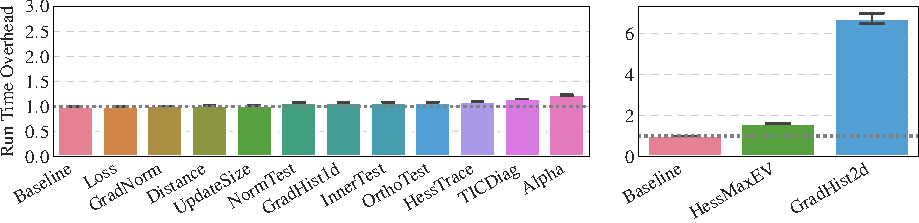
\includegraphics{../repos/cockpit-paper/fig/01_benchmark/output/fig_individual/benchmark_combined_mnist_logreg_cuda_thesis-wide}
    \label{cockpit::fig:app_benchmark_instruments_cuda-mnist_logreg}
  \end{subfigure}
  \vfill
  \begin{subfigure}[t]{\linewidth}
    \caption{Computational overhead for \mnist \mlp (GPU)}
    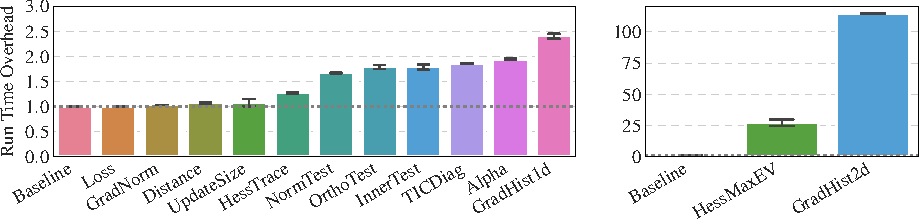
\includegraphics{../repos/cockpit-paper/fig/01_benchmark/output/fig_individual/benchmark_combined_mnist_mlp_cuda_thesis-wide}
    \label{cockpit::fig:app_benchmark_instruments_cuda-mnist_mlp}
  \end{subfigure}
  \vfill
  \begin{subfigure}[t]{\linewidth}
    \caption{Computational overhead for \cifarten \threecthreed (GPU)}
    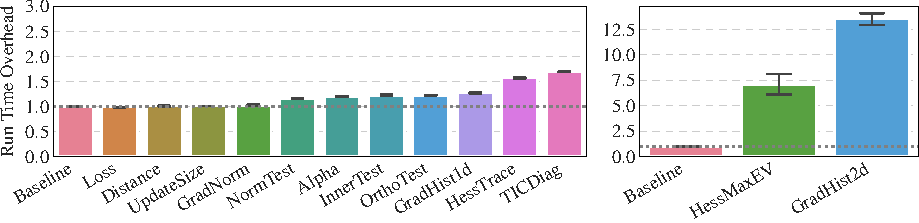
\includegraphics{../repos/cockpit-paper/fig/01_benchmark/output/fig_individual/benchmark_combined_cifar10_3c3d_cuda_thesis-wide}
    \label{cockpit::fig:app_benchmark_instruments_cuda-cifar10}
  \end{subfigure}
  \vfill
  \begin{subfigure}[t]{\linewidth}
    \caption{Computational overhead for \fmnist \twoctwod (GPU)}
    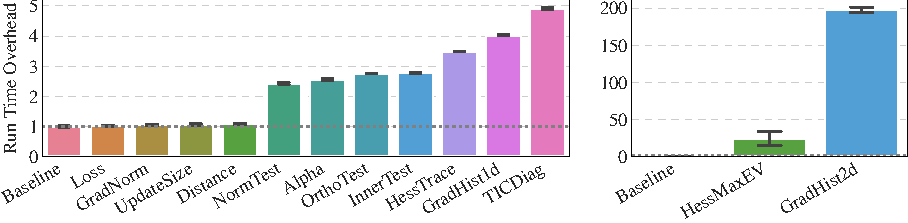
\includegraphics{../repos/cockpit-paper/fig/01_benchmark/output/fig_individual/benchmark_combined_fmnist_2c2d_cuda_thesis-wide}
    \label{cockpit::fig:app_benchmark_instruments_cuda-fmnist}
  \end{subfigure}
  \vfill
  \caption{\textbf{Individual overhead of \cockpittitle's instruments on GPU for
      four different problems.} All run times are shown as multiples of the
    \emph{baseline} without tracking. Expensive quantities are displayed in
    separate panels on the right. Experimental details in the text.}
  \label{cockpit::fig:app_benchmark_instruments_cuda}
\end{figure*}

\captionsetup[subfigure]{justification=centering, singlelinecheck=true}

%%% Local Variables:
%%% mode: latex
%%% TeX-master: "../../../thesis"
%%% End:


\captionsetup[subfigure]{justification=justified,singlelinecheck=false}

\begin{figure*}[p]
  \vfill
  \begin{subfigure}[t]{\linewidth}
    \caption{Computational overhead for \mnist \MNISTNET (CPU)}
    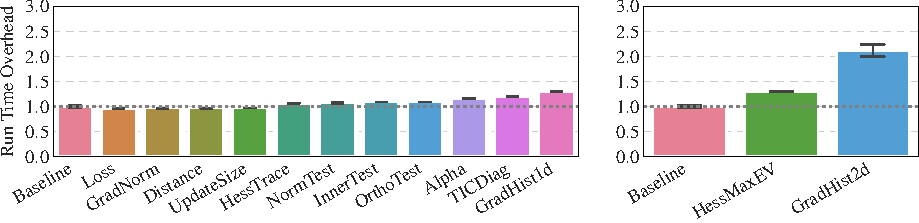
\includegraphics{../repos/cockpit-paper/fig/01_benchmark/output/fig_individual/benchmark_combined_mnist_logreg_cpu_thesis-wide}
    \label{cockpit::fig:app_benchmark_instruments_cpu-mnist_logreg}
  \end{subfigure}
  \vfill
  \begin{subfigure}[t]{\linewidth}
    \caption{Computational overhead for \mnist \mlp (CPU)}
    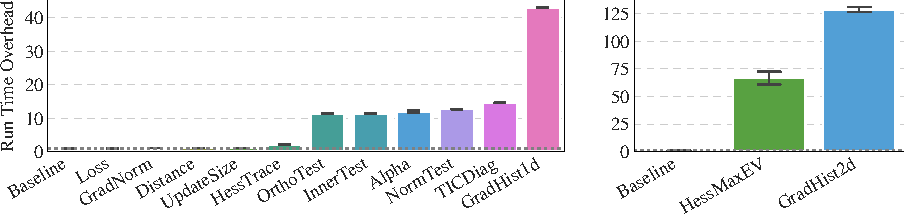
\includegraphics{../repos/cockpit-paper/fig/01_benchmark/output/fig_individual/benchmark_combined_mnist_mlp_cpu_thesis-wide}
    \label{cockpit::fig:app_benchmark_instruments_cpu-mnist_mlp}
  \end{subfigure}
  \vfill
  \begin{subfigure}[t]{\linewidth}
    \caption{Computational overhead for \cifarten \threecthreed (CPU)}
    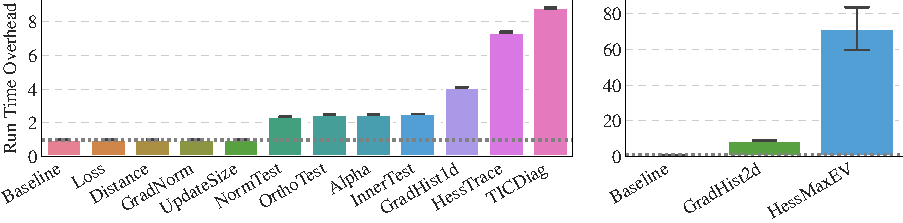
\includegraphics{../repos/cockpit-paper/fig/01_benchmark/output/fig_individual/benchmark_combined_cifar10_3c3d_cpu_thesis-wide}
    \label{cockpit::fig:app_benchmark_instruments_cpu-cifar10}
  \end{subfigure}
  \vfill
  \begin{subfigure}[t]{\linewidth}
    \caption{Computational overhead for \fmnist \twoctwod (CPU)}
    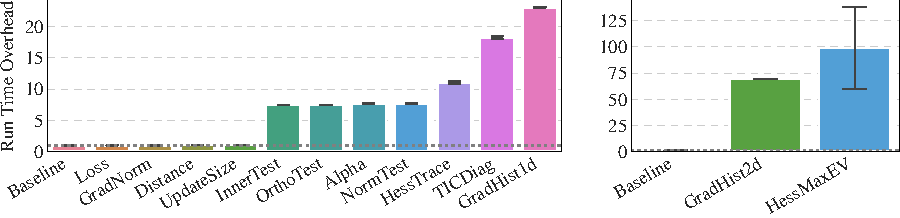
\includegraphics{../repos/cockpit-paper/fig/01_benchmark/output/fig_individual/benchmark_combined_fmnist_2c2d_cpu_thesis-wide}
    \label{cockpit::fig:app_benchmark_instruments_cpu-fmnist}
  \end{subfigure}
  \vfill
  \caption{\textbf{Individual overhead of \cockpittitle's instruments on CPU for
      four different problems.} All run times are shown as multiples of the
    \emph{baseline} without tracking. Expensive quantities are displayed in
    separate panels on the right. Experimental details in the text.}
  \label{cockpit::fig:app_benchmark_instruments_cpu}
\end{figure*}

\captionsetup[subfigure]{justification=centering, singlelinecheck=true}

%%% Local Variables:
%%% mode: latex
%%% TeX-master: "../../../thesis"
%%% End:


%%% Local Variables:
%%% mode: latex
%%% TeX-master: "../thesis"
%%% End:

\subsubsection{Configuration Overhead}\label{cockpit::app:benchmark-configuration}

For the estimation of different \cockpit configuration overheads, we use almost
the same setting as described above, training for $512$ iterations and tracking
only every specified interval.

\subsubsection{Configuration Overhead on GPU Versus CPU}

\Cref{cockpit::fig:app_benchmark_configurations_cuda} and
\Cref{cockpit::fig:app_benchmark_configurations_cpu} show the configuration
overhead for four different \deepobs problems. The bottom left part of
\Cref{cockpit::fig:app_benchmark_configurations_cuda} corresponds to
\Cref{cockpit::fig:benchmark_heatmap}. In general, increased parallelism can be
exploited on a GPU, leading to smaller overheads in comparison to a CPU.

\cockpit can even scale to significantly larger problems, such as a \resnetfifty
on \imagenet-like data.
\Cref{cockpit::fig:app_benchmark_configurations_gpu_imagenet} shows the
computational overhead for different tracking intervals on such a large-scale
problem. Using the \textit{economy} configuration, we can achieve our
self-imposed goal of at most doubling the run time even when tracking every
fourth step. More extensive configurations (such as the \textit{full} set) would
indeed have almost prohibitively large costs associated. However, these costs
could be dramatically reduced when one decides to only inspect a part of the
network using \cockpit. Note, individual gradients are not properly defined when
using batch norm, therefore, we replaced these batch norm layers with identity
layers when using the \resnetfifty.

\captionsetup[subfigure]{justification=justified,singlelinecheck=false}

\begin{figure*}[t]
  \centering
  \begin{subfigure}[t]{0.35\linewidth}
    \centering
    \caption{\mnist \MNISTNET (GPU)}
    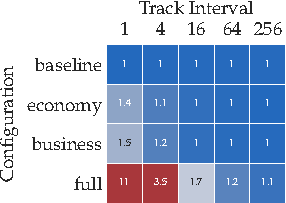
\includegraphics{../repos/cockpit-paper/fig/01_benchmark/output/fig_grid/benchmark_mnist_logreg_cuda_app_thesis-wide}
    \label{cockpit::fig:app_benchmark_configurations_cuda-mnist_logreg}
  \end{subfigure}
  \hspace{0.1\linewidth}
  \begin{subfigure}[t]{0.35\linewidth}
    \centering
    \caption{\mnist \mlp (GPU)}
    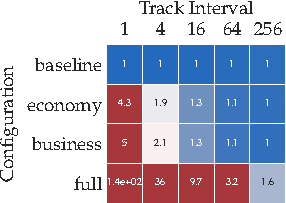
\includegraphics{../repos/cockpit-paper/fig/01_benchmark/output/fig_grid/benchmark_mnist_mlp_cuda_app_thesis-wide}
    \label{cockpit::fig:app_benchmark_configurations_cuda-mnist_mlp}
  \end{subfigure}
  \begin{subfigure}[t]{0.35\linewidth}
    \centering
    \caption{\cifarten \threecthreed (GPU)}
    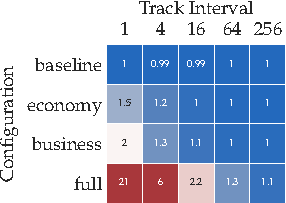
\includegraphics{../repos/cockpit-paper/fig/01_benchmark/output/fig_grid/benchmark_cifar10_3c3d_cuda_app_thesis-wide}
    \label{cockpit::fig:app_benchmark_configurations_cuda-cifar}
  \end{subfigure}
  \hspace{0.1\linewidth}
  \begin{subfigure}[t]{0.35\linewidth}
    \centering
    \caption{\fmnist \twoctwod (GPU)}
    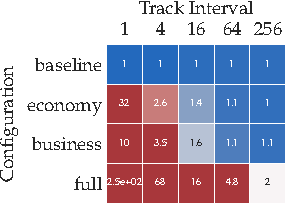
\includegraphics{../repos/cockpit-paper/fig/01_benchmark/output/fig_grid/benchmark_fmnist_2c2d_cuda_app_thesis-wide}
    \label{cockpit::fig:app_benchmark_configurations_cuda-fmnist}
  \end{subfigure}
  \caption{\textbf{Overhead of \cockpittitle configurations on GPU for four
      different problems with varying tracking interval.} Color bar is the same
    as in \autoref{cockpit::fig:benchmark}.}
  \label{cockpit::fig:app_benchmark_configurations_cuda}
\end{figure*}

\captionsetup[subfigure]{justification=centering, singlelinecheck=true}

%%% Local Variables:
%%% mode: latex
%%% TeX-master: "../../../thesis"
%%% End:


\captionsetup[subfigure]{justification=justified,singlelinecheck=false}

\begin{figure}[t]
	\centering
	\begin{subfigure}[t]{0.4\textwidth}
		\caption{\mnist Log.\,Reg.\,(CPU)}
		\includegraphics[width=\linewidth]{fig/01_benchmark/fig_grid/benchmark_mnist_logreg_cpu_app}
		\label{fig:app_benchmark_configurations_cpu-mnist_logreg}
	\end{subfigure}
	\hspace{0.06\textwidth}
	\begin{subfigure}[t]{0.4\textwidth}
		\caption{\mnist \mlp\,(CPU)}
		\includegraphics[width=\linewidth]{fig/01_benchmark/fig_grid/benchmark_mnist_mlp_cpu_app}
		\label{fig:app_benchmark_configurations_cpu-mnist_mlp}
		\vspace{0.25cm}
	\end{subfigure}
	\begin{subfigure}[t]{0.4\textwidth}
		\caption{\cifarten \threecthreed\,(CPU)}
		\includegraphics[width=\linewidth]{fig/01_benchmark/fig_grid/benchmark_cifar10_3c3d_cpu_app}
		\label{fig:app_benchmark_configurations_cpu-cifar}
	\end{subfigure}
	\hspace{0.06\textwidth}
	\begin{subfigure}[t]{0.4\textwidth}
		\caption{\fmnist \twoctwod\,(GPU)}
		\includegraphics[width=\linewidth]{fig/01_benchmark/fig_grid/benchmark_fmnist_2c2d_cpu_app}
		\label{fig:app_benchmark_configurations_cpu-fmnist}
	\end{subfigure}
	\caption{\textbf{Overhead of \cockpittitle configurations on CPU for four
			different problems with varying tracking interval.} Color bar is the same as in \autoref{fig:benchmark}.}
	\label{fig:app_benchmark_configurations_cpu}
\end{figure}

\captionsetup[subfigure]{justification=centering, singlelinecheck=true}

%%% Local Variables:
%%% mode: latex
%%% TeX-master: "../cockpit_paper"
%%% End:


\clearpage

\begin{figure}[t]
	\centering
	\includegraphics[width=0.59\linewidth]{fig/01_benchmark/fig_grid/benchmark_dummyimagenet_resnet50nobn_cuda_app}
	
	\caption{\textbf{Overhead of \cockpittitle configurations on GPU for \resnetfifty on
			\imagenet.} \cockpit's instruments scale efficiently even to very large problems
			(here: $1000$ classes, $(3, 224, 224)$-sized inputs, and a batch size of $64$.
			For individual gradients to be defined, we replaced the batch norm layers of the 
			\resnetfifty model with identities.) Color bar is the same as in \autoref{fig:benchmark}.}
	\label{fig:app_benchmark_configurations_gpu_imagenet}
\end{figure}


%%% Local Variables:
%%% mode: latex
%%% TeX-master: "../cockpit_paper"
%%% End:


%%% Local Variables:
%%% mode: latex
%%% TeX-master: "../thesis"
%%% End:

\subsection{Performance of Two-dimensional Histograms}\label{cockpit::app:histograms}

Both one- and two-dimensional histograms require $|\sB| \times D$ elements be
accessed, and hence perform similarly. However, we observed different behavior
on GPU and decided to omit the two-dimensional histogram's run time in the main
text. As explained here, this performance lack is not fundamental, but a
shortcoming of the GPU implementation. \pytorch provides built-in functionality
for computing one-dimensional histograms at the time of writing, but is not yet
featuring multi-dimensional histograms. We experimented with three
implementations:
\begin{itemize}
\item \textbf{\pytorch (third party):} A third party
  implementation\footnote{Permission granted by the authors of
    \href{cockpit::https://github.com/miranov25/RootInteractive/blob/7019e4c2b9f291551aeeb8677a969cfcfde690d1/RootInteractive/Tools/Histograms/histogramdd_pytorch.py}{\texttt{github.com/miranov25/.../histogramdd\_pytorch.py}}.}
  under review for being integrated into \pytorch\footnote{See
    \url{https://github.com/pytorch/pytorch/pull/44485}.}. It relies on
  \texttt{torch.bincount}, which uses \inlinecode{atomicAdd}s that represent a
  bottleneck for histograms where most counts are contained in one
  bin.\footnote{See
    \mbox{\url{https://discuss.pytorch.org/t/torch-bincount-1000x-slower-on-cuda/42654}}}
  This occurs often for over-parameterized deep models, as most of the gradient
  elements are zero.

\item \textbf{\pytorch (\cockpittitle):} Our implementation uses a workaround,
  computes bin indices and scatters the counts into their associated bins with
  \inlinecode{torch.Tensor.put\_}. This circumvents \inlinecode{atomicAdd}s, but
  has poor memory locality.

\item \textbf{\numpy:} The single-threaded \inlinecode{numpy.histogram2d} serves
  as baseline, but does not run on GPUs.
\end{itemize}


% pgfplots style "histogrambenchmarkdefault"
\pgfkeys{/pgfplots/histogrambenchmarkdefault/.style={
    enlarge x limits=-0.05,
    width=1.0\linewidth,
    height=0.7\linewidth,
    every axis plot/.append style={line width = 1.5pt},
    tick pos = left,
    ylabel near ticks,
    xlabel near ticks,
    xtick align = inside,
    ytick align = inside,
    legend cell align = left,
    legend columns = 1,
    % legend pos = south east,
    legend style = {
      fill opacity = 0.7,
      text opacity = 1,
      font = \footnotesize,
    },
    xticklabel style = {font = \footnotesize, inner xsep = -5ex},
    xlabel style = {font = \footnotesize},
    axis line style = {black},
    yticklabel style = {font = \footnotesize, inner ysep = -4ex},
    ylabel style = {font = \footnotesize},
    title style = {font = \footnotesize, inner ysep = -3ex},
    grid = major,
    grid style = {dashed}
  }
}

\begin{figure*}
  \begin{subfigure}[t]{0.49\linewidth}
    \pgfkeys{/pgfplots/zmystyle/.style={histogrambenchmarkdefault,
        xlabel={Histogram Balance $b$}
      }}
    \caption{GPU}
    \tikzexternalenable
    % This file was created by tikzplotlib v0.9.3.
\begin{tikzpicture}

\definecolor{color0}{rgb}{0.12156862745098,0.466666666666667,0.705882352941177}
\definecolor{color1}{rgb}{1,0.498039215686275,0.0549019607843137}

\begin{axis}[
axis line style={white!80!black},
legend style={fill opacity=0.8, draw opacity=1, text opacity=1, draw=white!80!black},
tick pos=left,
xlabel={Histogram Balance},
xmin=-0.039, xmax=1.039,
ylabel={Run Time [s]},
ymin=0.0647793941403482, ymax=344.025767453251,
ymode=log,
zmystyle
]
\addplot [, color0, dashed]
table {%
0.01 4.54533004760742
0.0615789473684211 2.08099224567413
0.113157894736842 0.744264936447144
0.164736842105263 0.445815587043762
0.216315789473684 0.335660696029663
0.267894736842105 0.282471227645874
0.319473684210526 0.253187036514282
0.371052631578947 0.232630848884583
0.422631578947368 0.219761872291565
0.474210526315789 0.210704207420349
0.52578947368421 0.206429862976074
0.577368421052632 0.218602991104126
0.628947368421053 0.214805579185486
0.680526315789474 0.20776104927063
0.732105263157895 0.20455629825592
0.783684210526316 0.20727813243866
0.835263157894737 0.206504940986633
0.886842105263158 0.203398704528809
0.9 0.20402295589447
0.938421052631579 0.204293870925903
0.99 0.204171013832092
};
\addlegendentry{\textsc{PyTorch} (\textsc{Cockpit})}
\addplot [, color1, dashed]
table {%
0.01 232.951647591591
0.0615789473684211 67.0944833517075
0.113157894736842 12.7715488433838
0.164736842105263 5.53443562984467
0.216315789473684 2.58965411186218
0.267894736842105 1.4656699180603
0.319473684210526 0.907050752639771
0.371052631578947 0.633884406089783
0.422631578947368 0.44161102771759
0.474210526315789 0.332058143615723
0.52578947368421 0.243267822265625
0.577368421052632 0.193850588798523
0.628947368421053 0.160495829582214
0.680526315789474 0.137686920166016
0.732105263157895 0.118721318244934
0.783684210526316 0.105425000190735
0.835263157894737 0.106805515289307
0.886842105263158 0.108340263366699
0.9 0.105959153175354
0.938421052631579 0.103169775009155
0.99 0.0956669807434082
};
\addlegendentry{\textsc{PyTorch} (third party)}
\end{axis}

\end{tikzpicture}

    \tikzexternaldisable
    \label{cockpit::fig:app-histogram2d-benchmark-gpu}
  \end{subfigure}
  \hfill
  \begin{subfigure}[t]{0.49\linewidth}
    \pgfkeys{/pgfplots/zmystyle/.style={histogrambenchmarkdefault,
        xlabel={Histogram Balance $b$}
      }}
    \caption{CPU}
    \tikzexternalenable
    % This file was created by tikzplotlib v0.9.3.
\begin{tikzpicture}

\definecolor{color0}{rgb}{0.12156862745098,0.466666666666667,0.705882352941177}
\definecolor{color1}{rgb}{1,0.498039215686275,0.0549019607843137}
\definecolor{color2}{rgb}{0.172549019607843,0.627450980392157,0.172549019607843}

\begin{axis}[
axis line style={white!80!black},
legend style={fill opacity=0.8, draw opacity=1, text opacity=1, at={(0.91,0.5)}, anchor=east, draw=white!80!black},
tick pos=left,
xlabel={Histogram Balance},
xmin=-0.039, xmax=1.039,
ylabel={Run Time [s]},
ymin=0.919387552518064, ymax=8.28341609861724,
ymode=log,
zmystyle
]
\addplot [, color0, dashed]
table {%
0.01 1.04204399585724
0.0615789473684211 1.03900332450867
0.113157894736842 1.07859117984772
0.164736842105263 1.06876609325409
0.216315789473684 1.04880547523499
0.267894736842105 1.04529702663422
0.319473684210526 1.05313646793365
0.371052631578947 1.06466472148895
0.422631578947368 1.06266655921936
0.474210526315789 1.05389556884766
0.52578947368421 1.06146202087402
0.577368421052632 1.04773416519165
0.628947368421053 1.06101129055023
0.680526315789474 1.04648265838623
0.732105263157895 1.0483683347702
0.783684210526316 1.04395830631256
0.835263157894737 1.04497628211975
0.886842105263158 1.04231572151184
0.9 1.04766194820404
0.938421052631579 1.04687905311584
0.99 1.0437038898468
};
\addlegendentry{\textsc{PyTorch} (\textsc{Cockpit})}
\addplot [, color1, dashed]
table {%
0.01 1.02336490154266
0.0615789473684211 1.02175369262695
0.113157894736842 1.02237765789032
0.164736842105263 1.02118575572968
0.216315789473684 1.01996810436249
0.267894736842105 1.02348549365997
0.319473684210526 1.0248743057251
0.371052631578947 1.02083847522736
0.422631578947368 1.01863925457001
0.474210526315789 1.02599215507507
0.52578947368421 1.0236154794693
0.577368421052632 1.02260437011719
0.628947368421053 1.03915128707886
0.680526315789474 1.03184995651245
0.732105263157895 1.0255656003952
0.783684210526316 1.0171329498291
0.835263157894737 1.02414612770081
0.886842105263158 1.02574753761292
0.9 1.01600201129913
0.938421052631579 1.01842267513275
0.99 1.02955875396729
};
\addlegendentry{\textsc{PyTorch} (third party)}
\addplot [, color2, dashed]
table {%
0.01 3.44840505123138
0.0615789473684211 3.95587799549103
0.113157894736842 4.67446537017822
0.164736842105263 4.98263554573059
0.216315789473684 5.3127799987793
0.267894736842105 5.58865821361542
0.319473684210526 5.89873046875
0.371052631578947 6.09700152873993
0.422631578947368 6.21813678741455
0.474210526315789 6.48546359539032
0.52578947368421 6.69456965923309
0.577368421052632 6.80199146270752
0.628947368421053 6.89959270954132
0.680526315789474 7.07993612289429
0.732105263157895 7.23664236068726
0.783684210526316 7.27940900325775
0.835263157894737 7.2930465221405
0.886842105263158 7.35840466022491
0.938421052631579 7.44740259647369
0.99 7.4957230091095
};
\addlegendentry{\textsc{NumPy} (single thread)}
\end{axis}

\end{tikzpicture}

    \tikzexternaldisable
    \label{cockpit::fig:app-histogram2d-benchmark-cpu}
  \end{subfigure}
  \caption{\textbf{Performance of two-dimensional histogram GPU implementations
      depends on the data.} (\subref{cockpit::fig:app-histogram2d-benchmark-gpu}) Run
    time for two different GPU implementations with histograms of different
    imbalance. \cockpit's implementation outperforms the third party solution by
    more than one order of magnitude in the deep learning regime ($b \ll 1$).
    (\subref{cockpit::fig:app-histogram2d-benchmark-cpu}) On CPU, performance is robust
    to histogram balance. The run time difference between \numpy and \pytorch is
    due to multi-threading. Data has the same size as \deepobs's \cifarten
    \threecthreed problem ($D =895,210, |\sB| = 128$). Curves represent averages
    over 10 independent runs. Error bars are omitted to improve legibility.}
  \label{cockpit::fig:app-histogram2d-benchmark}
\end{figure*}

To demonstrate the strong performance dependence on the data, we generate data
from a uniform distribution over $[0, b]\times[0, b]$, where $b \in (0, 1)$
parametrizes the histogram's balance, and compute two-dimensional histograms on
$[0,1]\times [0, 1]$. \Cref{cockpit::fig:app-histogram2d-benchmark-gpu} shows a
clear increase in run time of both GPU implementations for more imbalanced
histograms. Note that even though our implementation outperforms the third party
by more than one order of magnitude in the deep neural network regime ($b \ll
1$), it is still considerably slower than a one-dimensional histogram (see
\Cref{cockpit::fig:app_benchmark_instruments_cuda} (c)), and even slower on GPU
than on CPU (\Cref{cockpit::fig:app-histogram2d-benchmark} (b)). As expected,
the CPU implementations do not significantly depend on the data
(\Cref{cockpit::fig:app-histogram2d-benchmark-cpu}). The performance difference
between \pytorch and \numpy is likely due to multi-threading versus
single-threading.

Although a carefully engineered histogram GPU implementation is currently not
available, we think it will reduce the computational overhead to that of a
one-dimensional histogram in future releases.

%%% Local Variables:
%%% mode: latex
%%% TeX-master: "../thesis"
%%% End:

\clearpage

\section{\cockpittitle View of Convex Stochastic Problems}\label{cockpit::app:convex-problems}
\begin{figure*}[!h]
  \centering \Cshadowbox{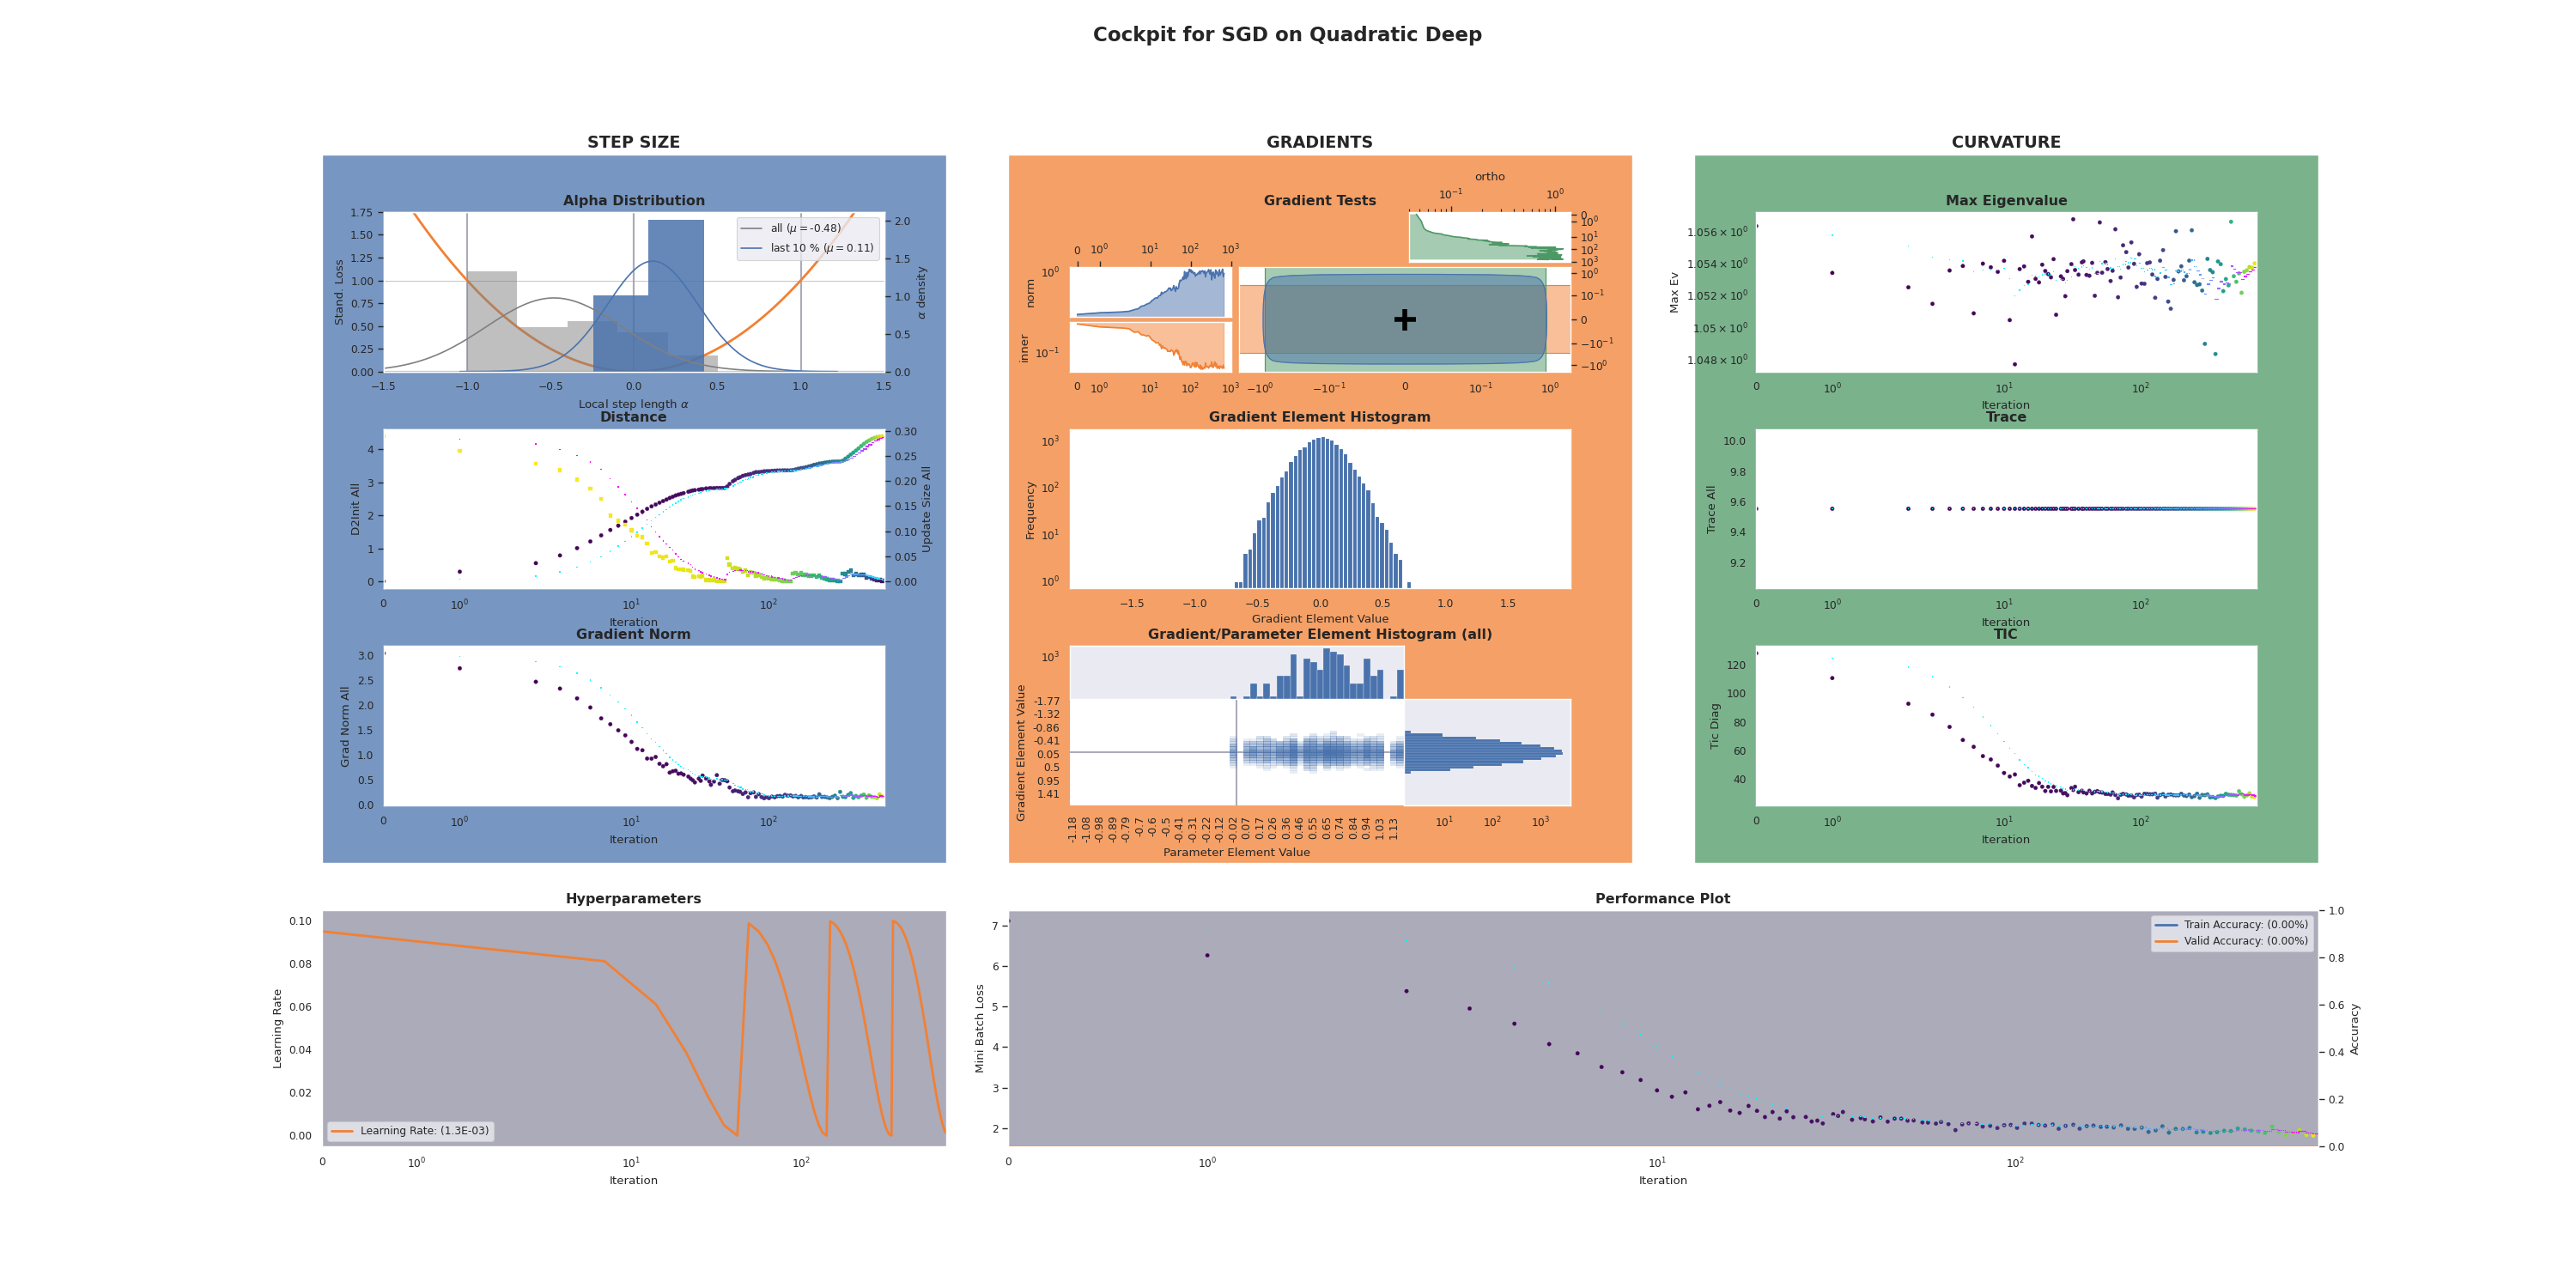
\includegraphics[width=.97\linewidth, trim={7cm 2.5cm
      5cm 0.5cm}, clip]{../repos/cockpit-paper/tex/fig/10_showcase/quadratic_deep_log.png}}

  \Cshadowbox{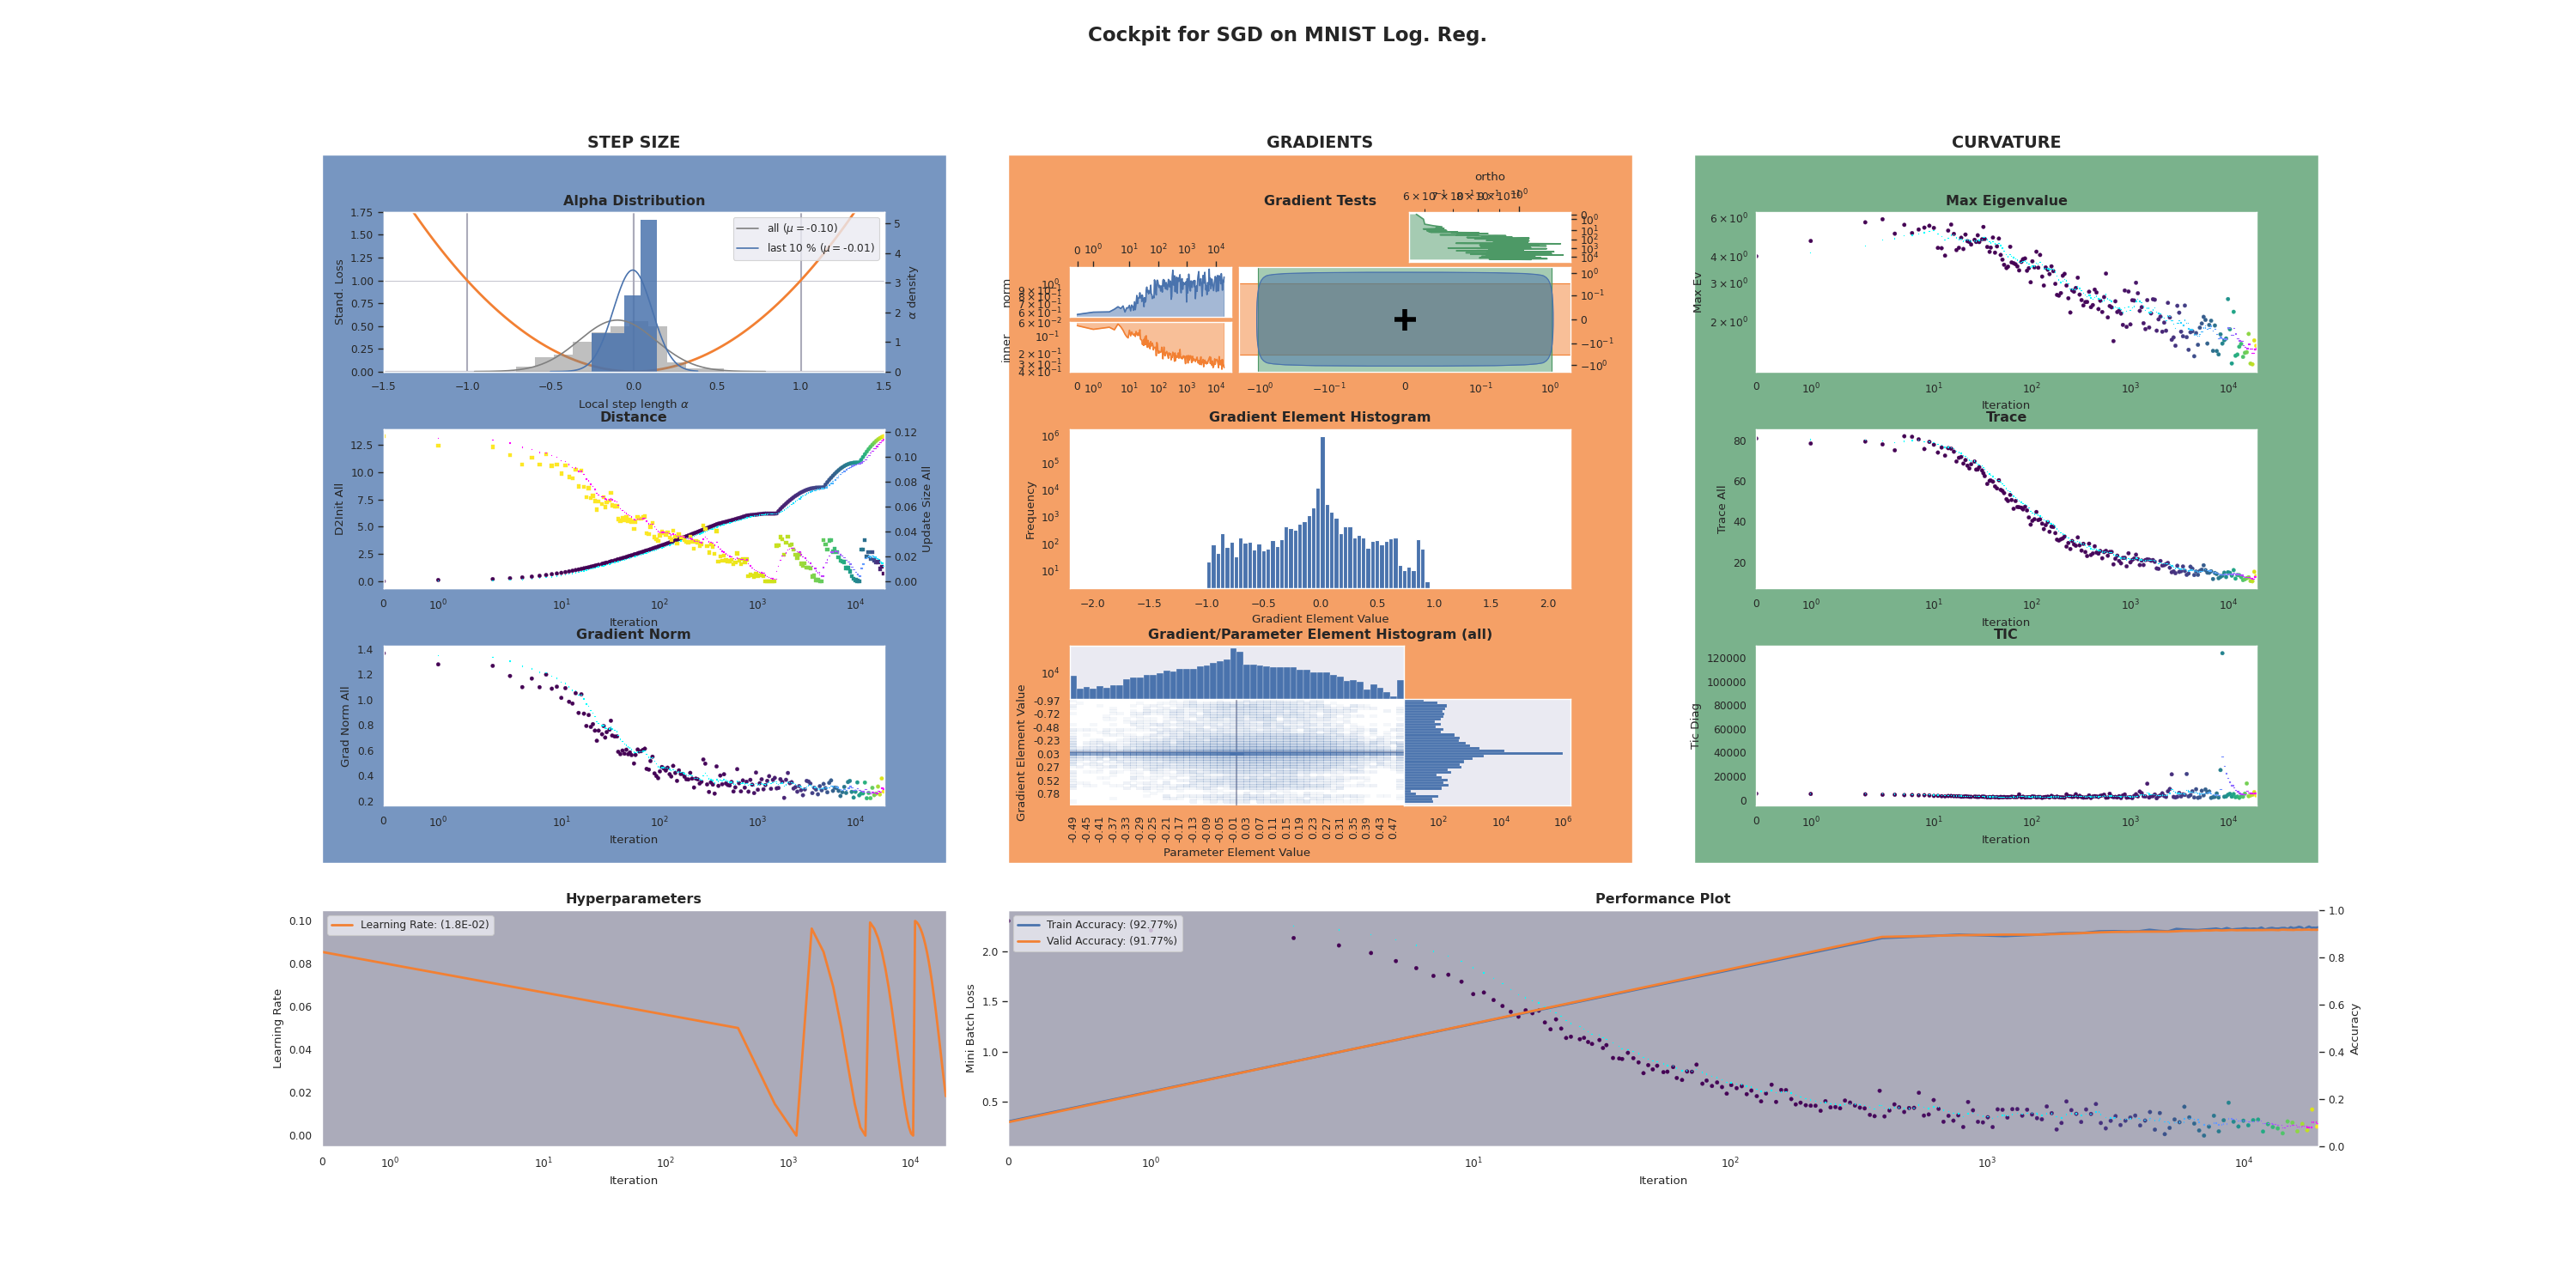
\includegraphics[width=.97\linewidth, trim={7cm 2.5cm 5cm 0.5cm},
    clip]{../repos/cockpit-paper/tex/fig/10_showcase/mnist_logreg_log.png}}

  \vspace{0.5\baselineskip}

  \caption{\textbf{Screenshot of \cockpittitle's full view for convex \deepobs
      problems.} Top \cockpit shows training on a noisy quadratic loss function.
    Bottom shows training on logistic regression on \mnist . Figure and labels
    are not meant to be legible. It is evident, that there is a fundamental
    difference in the optimization process, compared to training deep networks,
    \ie \Cref{cockpit::fig:showcase}. This is, for example, visible when comparing the
    gradient norms, which converge to zero for convex problems but not for deep
    learning.}\label{cockpit::fig:convex-problems}
\end{figure*}

%%% Local Variables:
%%% mode: latex
%%% TeX-master: "../thesis"
%%% End:


%%% Local Variables:
%%% mode: latex
%%% TeX-master: "../thesis"
%%% End:
